% ----------------------------------------------------------------------
% KNOWN ISSUES:
%
%   Currently only the 12pt size conforms to the UCSD requirements.
%   The 10pt and 11pt options make the footnote fonts too small.
%
%
% ----------------------------------------------------------------------
% HELP/CONTACT:
%
%   If you need help try the ucsd-thesis google group:
%   http://groups.google.com/group/ucsd-thesis
%
%
% ----------------------------------------------------------------------
% More control of the formatting of your thesis can be achieved through
% modifications of the included LaTeX class files:
%
%   * ucsd.cls    -- Class file
%   * uct10.clo   -- Configuration files for font sizes 10pt, 11pt, 12pt
%     uct11.clo                            
%     uct12.clo
%
% ----------------------------------------------------------------------



% Setup the documentclass 
% default options: 12pt, oneside, final
%
% fonts: 10pt, 11pt, 12pt -- are valid for UCSD dissertations.
% sides: oneside, twoside -- note that two-sided theses are not accepted 
%                            by OGS.
% mode: draft, final      -- draft mode switches to single spacing, 
%                            removes hyperlinks, and places a black box
%                            at every overfull hbox (check these before
%                            submission).
% chapterheads            -- Include this if you want your chapters to read:
%                              Chapter 1
%                              Title of Chapter
%
%                            instead of
%                              1 Title of Chapter
\documentclass[12pt,chapterheads]{ucsd}



% Include all packages you need here.  
% Some standard options are suggested below.
%
% See the project wiki for information on how to use 
% these packages. Other useful packages are also listed there.
%
%   http://code.google.com/p/ucsd-thesis/wiki/GettingStarted



\usepackage{amsmath, amscd, amssymb, amsthm}
\usepackage{graphicx}
\usepackage{subfigure}

%% TIMES FONT - replacements for Computer Modern
%%   This package will replace the default font with a
%%   Times-Roman font with math support.
% \usepackage[T1]{fontenc}
% \usepackage{mathptmx}

%% INDEX
%   Uncomment the following two lines to create an index: 
 \usepackage{makeidx}
 \makeindex
%   You will need to uncomment the \printindex line near the
%   bibliography to display the index.  Use the command
% \index{keyword} 
%   within the text to create an entry in the index for keyword.
%   To compile a LaTeX document with an index the 'makeindex'
%   command will need to be run.  See the wiki for more details.

%% HYPERLINKS
%   To create a PDF with hyperlinks, you need to include the hyperref package.
%   THIS HAS TO BE THE LAST PACKAGE INCLUDED!
%   Note that the options plainpages=false and pdfpagelabels exist
%   to fix indexing associated with having both (ii) and (2) as pages.
%   Also, all links must be black according to OGS.
%   See: http://www.tex.ac.uk/cgi-bin/texfaq2html?label=hyperdupdest
%   Note: This may not work correctly with all DVI viewers (i.e. Yap breaks).
%   NOTE: hyperref will NOT work in draft mode, as noted above.
% \usepackage[colorlinks=true, pdfstartview=FitV, 
%             linkcolor=black, citecolor=black, 
%             urlcolor=black, plainpages=false,
%             pdfpagelabels]{hyperref}
% \hypersetup{ pdfauthor = {Your Name Here}, 
%              pdftitle = {The Title of The Dissertation}, 
%              pdfkeywords = {Keywords for Searching}, 
%              pdfcreator = {pdfLaTeX with hyperref package}, 
%              pdfproducer = {pdfLaTeX} }

% defined by Jae
\usepackage{color}
\usepackage{multirow}
\usepackage{array}
\usepackage{rotating}
\usepackage{cite}

\newcommand{\CLs}{\ensuremath{CL_\mathrm{s}}}
\newcommand{\CLb}{\ensuremath{CL_\mathrm{b}}}
\newcommand{\CLsb}{\ensuremath{CL_\mathrm{s+b}}}

\newcommand{\MeV}{\ensuremath{\mathrm{Me\kern -0.1em V}}}
\newcommand{\GeV}{\ensuremath{\mathrm{Ge\kern -0.1em V}}}
\newcommand{\TeV}{\ensuremath{\mathrm{Te\kern -0.1em V}}}
\newcommand{\TeVcc}{\ensuremath{\,\mathrm{Te\kern -0.1em V\!/c}^2}}
\newcommand{\GeVcc}{\ensuremath{\,\mathrm{Ge\kern -0.1em V\!/c}^2}}
\newcommand{\MeVcc}{\ensuremath{\,\mathrm{Me\kern -0.1em V\!/c}^2}}
\newcommand{\GeVc}{\ensuremath{\mathrm{Ge\kern -0.1em V}\!/c}}
\newcommand{\nanob}{\mbox{{\rm ~nb}~}}
\newcommand{\fb}{\ensuremath{\mathrm{fb}}}
\newcommand{\pb}{\ensuremath{\mathrm{pb}}}
\newcommand{\ifb}{\ensuremath{\mathrm{fb^{-1}}}}
\newcommand{\ipb}{\ensuremath{\mathrm{pb^{-1}}}}
\newcommand{\grad}{\ensuremath{^{\circ}}}
%
% Special user made math symbols
%
\newcommand{\lsim}{\raisebox{-1.5mm}{$\:\stackrel{\textstyle{<}}{\textstyle{\sim}}\:$}}
\newcommand{\gsim}{\raisebox{-1.5mm}{$\:\stackrel{\textstyle{>}}{\textstyle{\sim}}\:$}}

% particles

\newcommand{\pipm}{\ensuremath{\pi^{\pm}}}
\newcommand{\pizero}{\ensuremath{\pi^{0}}}
\newcommand{\Hi}{\ensuremath{\mathrm{H}}}
\newcommand{\W}{\ensuremath{\mathrm{W}}}
\newcommand{\Wjets}{\ensuremath{\mathrm{W+jets}}}
\newcommand{\Zjets}{\ensuremath{\mathrm{Z+jets}}}
\newcommand{\Wt}{\ensuremath{\mathrm{Wt}}}
\newcommand{\Wstar}{\ensuremath{\mathrm{W}^{*}}}
\newcommand{\Wparenthesisstar}{\ensuremath{\mathrm{W}^{(*)}}}
\newcommand{\WW}{\ensuremath{\W^+\W^-}}
\newcommand{\Z}{\ensuremath{\mathrm{Z}}}
\newcommand{\Zstar}{\ensuremath{\mathrm{Z}^{*}}}
\newcommand{\Astar}{\ensuremath{\mathrm{\gamma}^{*}}}
\newcommand{\ZZ}{\ensuremath{\Z\Z}}
\newcommand{\WZ}{\ensuremath{\W\Z}}
\newcommand{\Wgstar}{\ensuremath{\W\Astar}}
\newcommand{\WgstarEE}{\ensuremath{\W\Astar\to\ell\nu ee}}
\newcommand{\WgstarMM}{\ensuremath{\W\Astar\to\ell\nu\mu\mu}}
\newcommand{\Zgstar}{\ensuremath{\Z\Astar}}
\newcommand{\ZgstarEE}{\ensuremath{\Z\Astar\to\ell\nu ee}}
\newcommand{\ZgstarMM}{\ensuremath{\Z\Astar\to\ell\nu\mu\mu}}
\newcommand{\E}{\ensuremath{\mathrm{e}}}
\newcommand{\Ep}{\ensuremath{\mathrm{e}^{+}}}
\newcommand{\Em}{\ensuremath{\mathrm{e}^{-}}}
\newcommand{\Epm}{\ensuremath{\mathrm{e}^{\pm}}}
\newcommand{\Emp}{\ensuremath{\mathrm{e}^{\mp}}}
\newcommand{\M}{\ensuremath{\mu}}
\newcommand{\Mp}{\ensuremath{\mu^{+}}}
\newcommand{\Mm}{\ensuremath{\mu^{-}}}
\newcommand{\Mpm}{\ensuremath{\mu^{\pm}}}
\newcommand{\Mmp}{\ensuremath{\mu^{\mp}}}
\newcommand{\Tau}{\ensuremath{\tau}}
\newcommand{\Nu}{\ensuremath{\nu}}
\newcommand{\Nubar}{\ensuremath{\bar{\nu}}}
\newcommand{\Lep}{\ensuremath{\ell}}
\newcommand{\Lepp}{\ensuremath{\ell^{+}}}
\newcommand{\Lepm}{\ensuremath{\ell^{-}}}
\newcommand{\Lprime}{\ensuremath{\Lep^{\prime}}}
\newcommand{\Prot}{\ensuremath{\mathrm{p}}}
\newcommand{\Pbar}{\ensuremath{\bar{\mathrm{p}}}}
\newcommand{\PP}{\Prot\Prot}
\newcommand{\PPbar}{\Prot\Pbar}
\newcommand{\ttbar}{\ensuremath{\mathrm{t}\bar{\mathrm{t}}}}
\newcommand{\qq}{\ensuremath{\mathrm{q}\mathrm{q}}}
%\newcommand{\bbbar}{\ensuremath{\mathrm{b}\bar{\mathrm{b}}}}
\newcommand{\Wtb}{\ensuremath{\W\mathrm{t}\mathrm{b}}}
\newcommand{\Top}{\ensuremath{\mathrm{t}}}
\newcommand{\Bot}{\ensuremath{\mathrm{b}}}
\newcommand{\Atop}{\ensuremath{\bar{\mathrm{t}}}}
\newcommand{\Abot}{\ensuremath{\bar{\mathrm{b}}}}
% arrow
\newcommand{\To}{\ensuremath{\rightarrow}}

% masses
\newcommand{\mHi}{\ensuremath{m_{\mathrm{H}}}}
\newcommand{\mW}{\ensuremath{m_{\mathrm{W}}}}
\newcommand{\mZ}{\ensuremath{m_{\mathrm{Z}}}}
\newcommand{\mll}{\ensuremath{m_{\Lep\Lep}}}
\newcommand{\mt}{\ensuremath{m_{\mathrm{T}}}}

% kinematics
\newcommand{\pt}{\ensuremath{p_\mathrm{T}}}
\newcommand{\ptveto}{\ensuremath{\pt^\mathrm{veto}}}
\newcommand{\ptl}{\ensuremath{p_\perp^{\Lep}}}
\newcommand{\ptlmax}{\ensuremath{p_{\mathrm{T}}^{\Lep,\mathrm{max}}}}
\newcommand{\ptlmin}{\ensuremath{p_{\mathrm{T}}^{\Lep,\mathrm{min}}}}
\newcommand{\met}{\ensuremath{\Et^{\mathrm{miss}}}}
\newcommand{\delphill}{\ensuremath{\Delta\phi_{\Lep\Lep}}}
\newcommand{\deletall}{\ensuremath{\Delta\eta_{\Lep\Lep}}}
\newcommand{\delphimetl}{\ensuremath{\Delta\phi_{\met\Lep}}}
\newcommand{\Et}{\ensuremath{E_\mathrm{T}}}
\newcommand{\delR}{\ensuremath{\Delta R}}
\newcommand{\Eta}{\ensuremath{\eta}}

%efficiencies
\newcommand{\effsig}{\ensuremath{\varepsilon_{\mathrm{bkg}}^{\mathrm{S}}}}
\newcommand{\effnorm}{\ensuremath{\varepsilon_{\mathrm{bkg}}^{\mathrm{N}}}}
\newcommand{\Nsig}{\ensuremath{N_{\mathrm{bkg}}^{\mathrm{S}}}}
\newcommand{\Nnorm}{\ensuremath{N_{\mathrm{bkg}}^{\mathrm{N}}}}

% processes
\newcommand{\dyee}{\ensuremath{Z/\gamma^*\to ee}}
\newcommand{\dymm}{\ensuremath{Z/\gamma^*\to\mu\mu}}
\newcommand{\dytt}{\ensuremath{Z/\gamma^*\to\tau\tau}}
\newcommand{\dyll}{\ensuremath{Z/\gamma^*\to\ell\ell}}
\newcommand{\dy}{\ensuremath{Z/\gamma^*}}
\newcommand{\zee}{\ensuremath{Z\to ee}}
\newcommand{\zmm}{\ensuremath{Z\to\mu\mu}}
\newcommand{\ztt}{\ensuremath{Z\to\tau\tau}}
%\newcommand{\ttbar}{\ensuremath{t\bar{t}}}
\newcommand{\ppww}{\ensuremath{pp \to W^+W^-}}
\newcommand{\wwll}{\ensuremath{WW\to \ell^+\ell^-}}
\newcommand{\wwlnln}{\ensuremath{W^+W^-\to \ell^+\nu \ell^-\bar{\nu}}}
\newcommand{\ww}{\ensuremath{WW}}
\newcommand{\wwpm}{\ensuremath{W^+W^-}}
\newcommand{\hww}{\ensuremath{H\to W^+W^-}}
\newcommand{\wz}{\ensuremath{WZ}}
\newcommand{\zz}{\ensuremath{ZZ}}
\newcommand{\wgamma}{\ensuremath{W\gamma}}
\newcommand{\wjets}{\ensuremath{W+}jets} 
\newcommand{\wjetse}{\ensuremath{W+}jets(e)} 
\newcommand{\wjetsm}{\ensuremath{W+}jets(\mu)} 
\newcommand{\tw}{\ensuremath{tW}} 
\newcommand{\singletopt}{\ensuremath{t} ($t$-chan)} 
\newcommand{\singletops}{\ensuremath{t} ($s$-chan)} 
\newcommand{\zx}{\ensuremath{\mathrm{DY/WZ/ZZ}}}
\newcommand{\zv}{\ensuremath{\mathrm{WZ/ZZ}}}
\newcommand{\z}{\ensuremath{\mathrm{Z}}}
\newcommand{\routin}{\ensuremath{R_{out/in}}}

%other 
\def\fixme{({\bf FixMe})}
\newcommand{\ee}{\ensuremath{ee}}
\newcommand{\emu}{\ensuremath{e\mu}}
\newcommand{\mue}{\ensuremath{\mu e}}
\def\mm{\ensuremath{\mu\mu}}

% integrated luminosity
\newcommand{\intlumiSevenTeV}{4.92~\ifb}
\newcommand{\intlumiEightTeV}{19.5~\ifb}

% ww cross section
\newcommand{\wwCrossSectionMeasurement}{\ensuremath{\sigma_{WW}  = 69.23 \pm 2.39~\mathrm{(stat.)} \pm 6.40~\mathrm{(syst.)} \pm 3.43~\mathrm{(lumi.)~pb}}}

%%%%%%%%%%%
%
\newcounter{myfootertablecounter}

\newcommand\myfootnotemark{%
  %\refstepcounter{footnote}%
  \addtocounter{footnote}{1}%
  \footnotemark[\thefootnote]%
}%

\newcommand\myfootnotetext[1]{%
  \addtocounter{myfootertablecounter}{1}
  \footnotetext[\value{myfootertablecounter}]{#1}
}

% from now on, myfootnote has to be used rather than footnote to
% adapt the myfootercounter
\newcommand\myfootnote[1]{%
  \addtocounter{myfootertablecounter}{1}
  \footnote{#1}
}%



\begin{document}



%% FRONT MATTER
%
%  All of the front matter.
%  This includes the title, degree, dedication, vita, abstract, etc..
%  Modify the file template_frontmatter.tex to change these pages.
%
%
% UCSD Doctoral Dissertation Template
% -----------------------------------
% http://ucsd-thesis.googlecode.com
%
%


%% REQUIRED FIELDS -- Replace with the values appropriate to you

% No symbols, formulas, superscripts, or Greek letters are allowed
% in your title.
%\title{Evidence of a new boson that decays to two W bosons 
%in the full leptonic final states in 24.4 $fb^{-1}$ at 
%center-of-mass energy of 7 and 8 TeV with Compact Muon Solenoid detector}
\title{
Evidence of a New Boson that Decays to Two W Bosons 
and a Study on Its Spin-parity Nature 
in the Full Leptonic Final States 
at 7 and 8 TeV Center-of-mass Energy 
with the Compact Muon Solenoid Detector
}
\author{Jae Hyeok Yoo}
\degreeyear{2014}

% Master's Degree theses will NOT be formatted properly with this file.
\degreetitle{Doctor of Philosophy} 

\field{Physics}
\chair{Professor Frank W\"urthwein}
% Uncomment the next line iff you have a Co-Chair
% \cochair{Professor Cochair Semimaster} 
%
% Or, uncomment the next line iff you have two equal Co-Chairs.
%\cochairs{Professor Chair Masterish}{Professor Chair Masterish}

%  The rest of the committee members  must be alphabetized by last name.
\othermembers{
Professor Claudio Campagnari\\
Professor Pamela Cosman \\
Professor Aneesh Manohar \\
Professor Avraham Yagil \\ 
}
\numberofmembers{4} % |chair| + |cochair| + |othermembers|


%% START THE FRONTMATTER
%
\begin{frontmatter}

%% TITLE PAGES
%
%  This command generates the title, copyright, and signature pages.
%
\makefrontmatter 

%% DEDICATION
%
%  You have three choices here:
%    1. Use the ``dedication'' environment. 
%       Put in the text you want, and everything will be formated for 
%       you. You'll get a perfectly respectable dedication page.
%   
%
%    2. Use the ``mydedication'' environment.  If you don't like the
%       formatting of option 1, use this environment and format things
%       however you wish.
%
%    3. If you don't want a dedication, it's not required.
%
%
\begin{dedication} 
  To two, the loneliest number since the number one.
\end{dedication}


% \begin{mydedication} % You are responsible for formatting here.
%   \vspace{1in}
%   \begin{flushleft}
% 	To me.
%   \end{flushleft}
%   
%   \vspace{2in}
%   \begin{center}
% 	And you.
%   \end{center}
% 
%   \vspace{2in}
%   \begin{flushright}
% 	Which equals us.
%   \end{flushright}
% \end{mydedication}



%% EPIGRAPH
%
%  The same choices that applied to the dedication apply here.
%
\begin{epigraph} % The style file will position the text for you.
  \emph{A careful quotation\\
  conveys brilliance.}\\
  ---Smarty Pants
\end{epigraph}

% \begin{myepigraph} % You position the text yourself.
%   \vfil
%   \begin{center}
%     {\bf Think! It ain't illegal yet.}
% 
% 	\emph{---George Clinton}
%   \end{center}
% \end{myepigraph}


%% SETUP THE TABLE OF CONTENTS
%
\tableofcontents
% \listoffigures  % Uncomment if you have any figures
% \listoftables   % Uncomment if you have any tables



%% ACKNOWLEDGEMENTS
%
%  While technically optional, you probably have someone to thank.
%  Also, a paragraph acknowledging all coauthors and publishers (if
%  you have any) is required in the acknowledgements page and as the
%  last paragraph of text at the end of each respective chapter. See
%  the OGS Formatting Manual for more information.
%
\begin{acknowledgements} 
 Thanks to whoever deserves credit for Blacks Beach, Porters Pub, and
 every coffee shop in San Diego. 

 Thanks also to hottubs.
\end{acknowledgements}


%% VITA
%
%  A brief vita is required in a doctoral thesis. See the OGS
%  Formatting Manual for more information.
%
\begin{vitapage}
\begin{vita}
  \item[2007] B.S. in Physics, Korea University 
  \item[2009] M.S. in Physics, Korea University 
  \item[2014] Ph.D. in Physics, University of California, San Diego 
\end{vita}
\begin{publications}
  \item Your Name, ``A Simple Proof Of The Riemann Hypothesis'', \emph{Annals of Math}, 314, 2007.
  \item Your Name, Euclid, ``There Are Lots Of Prime Numbers'', \emph{Journal of Primes}, 1, 300 B.C.
\end{publications}
\end{vitapage}


%% ABSTRACT
%
%  Doctoral dissertation abstracts should not exceed 350 words. 
%   The abstract may continue to a second page if necessary.
%
\begin{abstract}
  This dissertation will be abstract. 
\end{abstract}


\end{frontmatter}





%%%%%%%%%%%%%%%%%%%%%%%%%%%%%%%%%%%%%%%%%%%%%%%%%%%%%%%%%%
%%%%%%%%%%%%%%%%%%%%%% DISSERTATION %%%%%%%%%%%%%%%%%%%%%%
%%%%%%%%%%%%%%%%%%%%%%%%%%%%%%%%%%%%%%%%%%%%%%%%%%%%%%%%%%

%
\chapter{Higgs Boson in Standard Model}
\label{ch:intro_higgs}
%%%%%%%%%%%%%%%%%%%%%%%%%%%%%%%%%%%%%%%%%%%%%%%%%%%%%%%%%%%%%%%%
\section{Higgs Mechanism}

%There are four forces in nature, gravity, electromagnetism, weak force 
%and strong force. Gravity is described by general relativity. 
Properties of elementary particles in nature and their interactions(forces)
with each other are described by the Standard 
Model(SM)~\cite{Glashow:1961tr,Weinberg:1967tq,Salam:1963tr} 
in particle physics. It is 
based on the gauge symmetry and the group structure of 
$\textrm{SU(3)}_\textrm{c} \otimes \textrm{SU(2)}_\textrm{L} 
\otimes \textrm{U(1)}_\textrm{Y}$, where  $\textrm{SU(3)}_\textrm{c}$, 
$\textrm{SU(2)}_\textrm{L}$ and $\textrm{U(1)}_\textrm{Y}$  
describe color, weak iso-spin and hyper charge, respectively. 
The gauge symmetry requires the weak gauge bosons to be massless,
but experimentally we know that Weak gauge bosons, $W^\pm$ and $Z$ are massive. 
The cure for this is the Higgs 
mechanism~\cite{Englert:1964et,Higgs:1964ia,Higgs:1964pj,Guralnik:1964eu,Higgs:1966ev, Kibble:1967sv}
based on the spontaneous symmetry breaking(SSB)
which breaks $\textrm{SU(2)}_\textrm{L} \otimes \textrm{U(1)}_\textrm{Y}$
to $\textrm{U(1)}_{\textrm{EM}}$. It gives masses to weak bosons but keeps photon massless. 
%\textcolor{red}{Explain why fermions are massless in SM before SSB, 
%and how they acquire their masses via interaction with Higgs field.
%page 93 of Gordon's book
%}


\subsection{How particles become massive : Higgs Mechanism}
Since Electroweak(EWK) theory is based on SU(2) symmetry, the Higgs field is 
given as a SU(2) doublet, 
\begin{eqnarray} 
\phi = \left(  \begin{array}{c} \phi^+ \\ \phi^0 \end{array} \right)
\end{eqnarray} 
where each element is a complex field, 
\begin{eqnarray} 
\phi^+ = \frac{\phi_1 + i\phi_2}{\sqrt{2}} 
\qquad \textrm{ and } \qquad  
\phi^0 = \frac{\phi_3 + i\phi_4}{\sqrt{2}}.
\end{eqnarray} 
We start with the Higgs Lagrangian to understand the essence of 
spontaneous symmetry breaking(SSB) before making things more 
complicated. The full SM Lagrangian will be discussed later.  
The Higgs Lagrangian($\mathcal{L}_\phi$) is composed of the kinetic 
and the potential terms. 
\begin{eqnarray}
\label{eq:lagHiggs}
\mathcal{L}_\phi 
=
\underbrace{
    \left( \partial_\mu \phi \right)^\dagger \left( \partial^\mu \phi \right)
}_\text{kinetic term} 
- 
\underbrace{
    \left( \mu^2 \phi^\dagger \phi + \lambda \left( \phi^\dagger \phi \right)^2 \right)
}_\text{potential} 
\end{eqnarray} 
where $\mu^2<0$ and $\lambda>0$.
The potential term which is a function of $ \phi^\dagger \phi$ is invariant under 
SU(2) local gauge transformation, 
\begin{eqnarray} 
\phi(x) 
\rightarrow 
\phi(x)' = e^{i \vec{\alpha}(x) \cdot \frac{\vec{\sigma}}{2}} \phi(x),
\end{eqnarray} 
where $\vec{\alpha}(x)$ is a vector of parameters and  
$\vec{\sigma}$ is a vector of Pauli matrices,  
\begin{align*}
\sigma_1 = \begin{pmatrix} 0 & 1\\
                            1 & 0
            \end{pmatrix}, 
\quad 
\sigma_2 = \begin{pmatrix} 0 & -i\\
                            i & 0
            \end{pmatrix}
\quad 
\textrm{and} 
\quad 
\sigma_3 = \begin{pmatrix} 1 & 0\\
                            0 & -1
            \end{pmatrix}.
\end{align*}
The potential has the minimum at 
%$\displaystyle  \phi^\dagger \phi = -\frac{\mu^2}{2\lambda} = \frac{v^2}{2}$ where 
$ \phi^\dagger \phi = -\mu^2/2\lambda = v^2/2$ where 
$v$ is the vacuum expectation value of the Higgs field $\phi$.
Due to SU(2) symmetry, the choice of vacuum state is not definite 
as seen in the following equation, 
\begin{eqnarray} 
\phi^\dagger \phi 
= 
\frac{1}{2} \left( \phi_1^2 + \phi_2^2 + \phi_3^2 + \phi_4^2\right) 
=
\frac{v^2}{2} 
\end{eqnarray}
where there are 4 real variables with only one constraint. 
This leads to an appropriate choice of vacuum for the physics of interest. 
We choose the vacuum state, $\phi_0$, as 
\begin{eqnarray} 
\phi_0 = \frac{1}{\sqrt{2}} \left(  \begin{array}{c} 0 \\ v \end{array} \right)
\end{eqnarray} 
and expand around it by $H(x)$
\begin{eqnarray} 
\label{eq:HiggsfieldSSB}
\phi(x) = \frac{1}{\sqrt{2}} \left(  \begin{array}{c} 0 \\ v + H(x) \end{array} \right)
\end{eqnarray} 
where $H(x)$ is the physical Higgs field.  
In order to make the Lagrangian invariant under SU(2) transformation,
the derivative $\partial_\mu$ should be replaced by the covariant 
derivative $\mathcal{D}_\mu$,
\begin{eqnarray} 
\mathcal{D}_\mu 
= 
\partial_\mu - ig_1 \frac{Y}{2} B_\mu - ig_2 \frac{\vec{\sigma}}{2} \cdot \overrightarrow{W}_\mu. 
\end{eqnarray} 
$B_\mu$ and $\overrightarrow{W}_\mu$ are the vector fields needed for U(1) and 
SU(2) gauge invariance, respectively. 
The $g_1$ and $g_2$ are the couplings that decide the strength of the
interactions associated with $B_\mu$ and $\overrightarrow{W}_\mu$. 
$Y$(weak hypercharge) and $\vec{\sigma}/2$ are the generators for U(1) and SU(2), respectively. 
Putting this into the Lagrangian $\mathcal{L_\phi}$, the kinetic term contains 
\begin{eqnarray}
\label{eq:kintermHiggsLag}
%\left( \mathcal{D}_\mu \phi \right)^\dagger \left( \mathcal{D}^\mu \phi \right) 
%= ... + 
\phi^\dagger 
\left[ - ig_1 \frac{Y}{2} B^\mu
       - ig_2 \frac{\vec{\sigma}}{2} \cdot \overrightarrow{W}^\mu \right]^\dagger 
\left[ - ig_1 \frac{Y}{2} B^\mu
       - ig_2 \frac{\vec{\sigma}}{2} \cdot \overrightarrow{W}^\mu \right] 
\phi.  
\end{eqnarray}
In order to derive the masses of W and Z bosons, we use the vacuum state of Higgs field $\phi_0$
because masses are present even without dynamical fields.  
With $Y=1$ and $\displaystyle \phi = \frac{1}{\sqrt{2}} 
\left(  \begin{array}{c} 0 \\ v \end{array} \right)$, 
and writing explicitly in $2\times2$ matrices, equation.~(\ref{eq:kintermHiggsLag}) becomes 
\begin{eqnarray}
\label{eq:WZmass}
\begin{array}{ccc} \multicolumn{2}{c}{ \displaystyle \vspace{0.3cm}   
\frac{1}{8} \left| \left(  \begin{array}{cc} 
g_1 B_\mu + g_2 W_\mu^3     & g_2 (W_\mu^1 - iW_\mu^2) \\
g_2 (W_\mu^1 + iW_\mu^2)    & g_1 B_\mu - g_2 W_\mu^3 \end{array} \right) 
\left(  \begin{array}{c} 0 \\ v \end{array} \right) \right|^2 
} & \\ & \multicolumn{2}{l}{\hspace{2cm} \vspace{0.3cm} \displaystyle   
= \frac{v^2}{8} \left| \left(  \begin{array}{c} 
g_2 (W_\mu^1 - iW_\mu^2) \\
g_1 B_\mu - g_2 W_\mu^3 
\end{array} \right) \right|^2} \\  
& \multicolumn{2}{l}{\hspace{2cm}  \displaystyle   
=   
\frac{v^2 g_2^2}{8} \left[ \left( W_\mu^1 \right)^2  + \left( W_\mu^2 \right)^2 \right] 
+ \frac{v^2}{8} \left( g_1 B_\mu - g_2 W_\mu^3 \right)^2.
} \end{array}    
\end{eqnarray} 
The first term can be re-written using charge states, 
$\displaystyle W^\pm = \frac{1}{\sqrt{2}} \left( W^1 \mp iW^2 \right)$, 
\begin{eqnarray}
\frac{1}{2} \left( \frac{v g_2}{2} \right)^2 
\left[ \left( W_\mu^+ \right)^2  + \left( W_\mu^- \right)^2 \right]. 
\end{eqnarray}
Thus, we have the mass of charged W boson $\displaystyle m_W = \frac{v g_2}{2}$.
Now we know that the second term in equation~(\ref{eq:WZmass}) should correspond to 
Z boson because that is the only remaining massive boson. Imposing the same 
normalization to the mixed field as the unmixed fields, the physical field for 
Z boson, $Z_\mu$, is given by
\begin{eqnarray} 
Z_\mu = \frac{\left( g_1 B_\mu - g_2 W_\mu^3 \right)}{\sqrt{g_1^2+g_2^2}}  
\end{eqnarray} 
which gives its mass, $\displaystyle m_Z = \frac{v}{2} \sqrt{g_1^2+g_2^2}$. 

There is a massless field orthogonal to $Z_\mu$,  
\begin{eqnarray} 
A_\mu = \frac{\left( g_1 B_\mu + g_2 W_\mu^3 \right)}{\sqrt{g_1^2+g_2^2}}  
\end{eqnarray}
It does not appear in the Lagrangian because its mass therm is zero.
This is the field that remains unbroken by SSB. So, it corresponds to the photon. 
%Using the definition of weak mixing angle, $\theta_W$, 
%\begin{equation} 
%\sin \theta_W = \frac{g_1}{\sqrt{g_1^2+g_2^2}}, \textrm{ and } 
%\cos \theta_W = \frac{g_2}{\sqrt{g_1^2+g_2^2}}  
%\end{equation} 

Re-writing the potential term in equation~(\ref{eq:lagHiggs})
using the physical weak boson states, $W_\mu^\pm$ and $Z_\mu$,
and their masses, we have the following terms for interactions between Higgs and weak bosons,
\begin{eqnarray}
\begin{array}{ccc} \multicolumn{2}{c}{\displaystyle 
2\frac{m_W^2}{v} H(x) W^+_\mu W^-_\mu
+ \frac{m_Z^2}{v} H(x) \left( Z_\mu \right)^2
} & \\ & \multicolumn{2}{c}{\hspace{2cm} \displaystyle
+ \frac{m_W^2}{v^2} H(x)^2 W^+_\mu W^-_\mu 
+\frac{m_Z^2}{2v^2} H(x)^2 \left( Z_\mu \right)^2.
} \end{array}   
\end{eqnarray} 
For Higgs-Weak boson interactions, the couplings are proportional to the square 
of weak boson mass.
\begin{figure}[htp]
\centering
\vspace{1cm}
\subfigure[H-VV interaction]{
\centering
\label{subfig:fd_HVV}
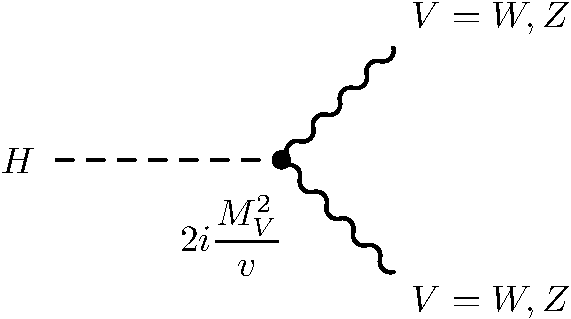
\includegraphics[height=3.5cm]{figures/FD_HVVterm.pdf}
}
\hspace{1cm}
\subfigure[HH-VV interaction]{
\centering
\label{subfig:fd_HHVV}
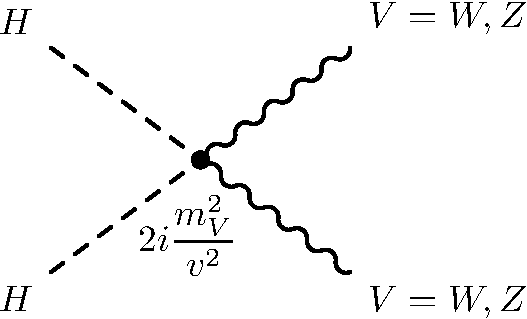
\includegraphics[height=3.5cm]{figures/FD_HHVVterm.pdf}
}
\caption{ Feynman diagrams for (a) H-VV and (b) HH-VV interactions.
}
\vspace{0.5cm}
\label{fig:fd_HVterm}
\end{figure}
The corresponding Feynman diagrams are shown in Figure~\ref{fig:fd_HVterm}. 
Considering additional factorials due to identical particles, the 
vertex factors can be written as $\displaystyle 2i \frac {m_V^2}{v}$ 
and $\displaystyle 2i \frac{m_V^2}{v^2}$ for H-VV and HH-VV vertices, respectively, 
where V denotes W or Z. 

After SSB, the Higss potential term,  
$\mu^2 \phi^\dagger \phi + \lambda \left( \phi^\dagger \phi \right)^2 $,
in the Lagrangian becomes 
\begin{eqnarray} 
\mathcal{L}_{\textrm{Higgs Potential}}
&=&   
\mu^2 \phi^\dagger \phi + \lambda \left( \phi^\dagger \phi \right)^2 \\ 
&=&   
\frac{\mu^2}{2} ( v + H )^2 + \frac{\lambda}{4} ( v + H )^4 \\ 
%&=&   
%\frac{\mu^2}{2} ( v^2 + H^2 + 2vH ) 
%+ \frac{\lambda}{4} ( v^4 + H^4 + 4v^2H^2 + 2v^2H^2 + 4vH^3 + 4v^3H) \\ 
&=& 
\label{eq:HiggsPontential}
... - \mu^2 H^2 - \frac{\mu^2}{v} H^3  - \frac{\mu^2}{4v^2} H^4 
\end{eqnarray} 
where $H^0$ and $H^1$ terms are ignored in the last line
because they are irrelevant in S-matrix calculations. 
%\textcolor{red}{I remember that the first order term does not 
%affect the lagrangian, but do not remember the argument.}
From equation~(\ref{eq:HiggsPontential}), the Higgs mass is identified 
as $\mHi^2 =  -2\mu^2$. %= 2\lambda v^2$.
Using this definition, equation~(\ref{eq:HiggsPontential}) becomes 
\begin{eqnarray} 
\mathcal{L}_{\textrm{Higgs Potential}}
&=& 
... - \frac{1}{2} \mHi^2 H^2 - \frac{\mHi^2}{2v} H^3  - \frac{\mHi^2}{8v^2} H^4    
\end{eqnarray}
The corresponding Feynman diagrams are shown in Figure~\ref{fig:fd_Hselfterm}. 
%
\begin{figure}[htp]
\centering
\vspace{1cm}
\subfigure[$\textrm{H}^3$ interaction]{
\centering
\label{subfig:fd_HHH}
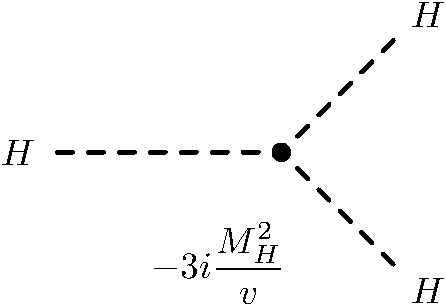
\includegraphics[height=3.5cm]{figures/FD_HHHterm.pdf}
}
\hspace{1cm}
\subfigure[$\textrm{H}^4$ interaction]{
\centering
\label{subfig:fd_HHHH}
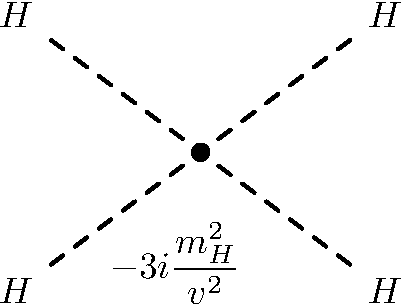
\includegraphics[height=3.5cm]{figures/FD_HHHHterm.pdf}
}
\caption{ Feynman diagrams for (a) $\textrm{H}^3$ and (b) $\textrm{H}^4$ interactions.
}
\vspace{0.5cm}
\label{fig:fd_Hselfterm}
\end{figure}

Now we see that the entire Higgs sector depends on only \mHi\ and $v$.
The $v$ is calculated by $v = \left( \sqrt{2} \gf \right)^{-1/2} = 246~\GeV$  
where $\gf$ is the Fermi constant which is extracted from measurement 
of muon lifetime. 
% \gf meausurement : http://www.sciencedirect.com/science/article/pii/S0168900201012839
Thus, the SM Higgs sector is fully described by \mHi. 
\mHi\ is a function of $\lambda$ and $v$($\mHi^2 = 2 \lambda v^2$)
and we do not know the physical meaning of $\lambda$, so 
the mass of Higgs boson is not predictable by theory.
It's experimentalists' task to measure \mHi\ and 
complete the Standard Model of particle physics.

The introduced Higgs field had 4 degrees of freedom, $\phi_1, \phi_2, \phi_3$ 
and $\phi_4$ before SSB. But, we chose the Higgs field to have only one degree 
of freedom, $H(x)$.  Where did the three go? 
By breaking $\textrm{SU(2)}_\textrm{L} \otimes \textrm{U(1)}_\textrm{Y}$ to $U(1)_{EM}$, 
the three gauge bosons acquired masses. This was done by adding longitudinal components 
to the three gauge bosons. As a result, we have only one physical Higgs field and 
three massive and one massless gauge bosons, instead of four unphysical 
Higgs fields and four massless gauge bosons.

The fermions acquire their masses by interacting with Higgs field. 
Let's start a discussion with leptons because the absence of right-handed neutrinos, 
\textit{i.e.} neutrinos are massless, makes the case simpler than quarks which 
have both right-handed and left-handed polarizations. 
%We can add SU(2)-invariant terms to the Lagrangian. 
\begin{table}[htb] 
\centering
\vspace{0.5cm} 
\caption{$\textrm{SU(2)}_\textrm{L} \otimes \textrm{U(1)}_\textrm{Y}$ quantum numbers.}
\vspace{0.5cm} 
\label{tab:su2Qnum}
\begin{tabular}{c c c}
\hline 
      & $T_3$ & Y \\
\hline \hline 
$\left(  \begin{array}{c} \nu_L \\ e_L \end{array} \right)$      & $\displaystyle  \frac{1}{2} $ & -1 \\
$ \nu_{R}$                                                      & 0 & 0 \\
$ e_R$                                                           & 0 & -2 \\
$\left(  \begin{array}{c} \phi_+  \\ \phi_0 \end{array} \right)$      & $\displaystyle  \frac{1}{2} $ & -1 \\
\hline 
\end{tabular}
\end{table}
Table~\ref{tab:su2Qnum} shows the quantum numbers of  
$\textrm{SU(2)}_\textrm{L} \otimes \textrm{U(1)}_\textrm{Y}$
for the left-handed electron doublet, right-handed neutrino, right-handed electron and 
Higgs doublet. Electron can be replaced by muon or tau leptons. 
From the table, one can see that the interaction such as 
\begin{eqnarray} 
e_R + \left(  \begin{array}{c} \phi_+  \\ \phi_0 \end{array} \right) 
\rightarrow 
\left(  \begin{array}{c} \nu_L \\ e_L \end{array} \right)
\end{eqnarray} 
conserves quantum numbers. Now the structure of the interaction is given, and
we specify its strength with $g_e$. Including the hermitian conjugate 
to the Lagrangian, the lepton-Higgs interaction term becomes 
\begin{eqnarray} 
\mathcal{L}_{int, lepton} 
&=& 
-g_e \left[ 
\left(  \begin{array}{cc} \bar{\nu}_L & \bar{e}_L \end{array} \right)
\left(  \begin{array}{c} \phi_+  \\ \phi_0 \end{array} \right) e_R
+ 
\bar{e}_R
\left(  \begin{array}{cc} \bar{\phi}_+  & \bar{\phi}_0 \end{array} \right) 
\left(  \begin{array}{c} \nu_L \\ e_L \end{array} \right)
\right].
\end{eqnarray} 
Using the chosen Higgs field in equation~(\ref{eq:HiggsfieldSSB}), 
%$\frac{1}{\sqrt{2}} \left(  \begin{array}{c} 0 \\ v + H(x) \end{array} \right)$, 
the Lagrangian is calculated to be 
\begin{eqnarray} 
\mathcal{L}_{int, lepton} 
&=& 
-\frac{g_e v}{\sqrt{2}}\left( \bar{e}_L e_R + \bar{e}_R e_L \right)  
-\frac{g_e H}{\sqrt{2}}\left( \bar{e}_L e_R + \bar{e}_R e_L \right). 
\end{eqnarray}
Since $\bar{e}e = \bar{e}(P_L^2+P_R^2)e = \bar{e}_L e_R + \bar{e}_R e_L$ where
$P_L$ and $P_R$ are projection operators, the first term, 
$\displaystyle -\frac{g_e v}{\sqrt{2}} \bar{e}e$, corresponds to the mass term for the electron. 
Thus, the mass is identified to be 
\begin{eqnarray} 
m_e = \frac{g_e v}{\sqrt{2}}.
\end{eqnarray} 
Rewriting the Lagrangian in terms of $m_e$ instead of an arbitrary $g_e$, we get 
\begin{eqnarray} 
\mathcal{L}_{int} 
&=& 
- m_e \bar{e}e  -\frac{m_e}{v} \bar{e}e H. 
\end{eqnarray} 
Since there isn't a physical motivation for $g_e$, $m_e$ is not calculable 
by theory, but needs to be determined by experiments. The second term 
corresponds to lepton-Higgs interaction. The size of the interaction 
is proportional to the mass of electrons. Thus, light leptons have very 
weak couplings to the Higgs field. For example, electron has 
%$\displaystyle \frac{m_e}{v} = \frac{0.5~\MeV}{246~\GeV} \sim \mathcal{O}\left(10^{-6}\right)$
%and muon has $\displaystyle \frac{106~\MeV}{246~\GeV} \sim \mathcal{O}\left(10^{-3}\right)$.
$m_e/v = 0.5~\MeV/246~\GeV \sim \mathcal{O}\left(10^{-6}\right)$
and muon has $m_\mu / v = 106~\MeV/246~\GeV \sim \mathcal{O}\left(10^{-3}\right)$.

The case for quarks is more complicated due to the presence of right-handed up-type 
quarks as opposed to the lepton case. In order to generate masses for up-type 
quarks, we need a new Higgs doublet 
\begin{eqnarray} 
\phi_c 
= i \sigma_2 \phi^* 
=  \left(  \begin{array}{c} \phi_0^* \\ -\phi_- \end{array} \right) 
=  \frac{1}{\sqrt{2}} \left(  \begin{array}{c} v + H(x) \\ 0 \end{array} \right). 
\end{eqnarray} 
The new Higgs field is invariant under $\textrm{SU(2)}_\textrm{L}$ transformation and has Y = -1. 
\begin{eqnarray} 
\mathcal{L}_{int, quark} 
&=& 
\begin{array}{ccc} \multicolumn{2}{c}{\displaystyle 
-g_{d} \left[ 
\left(  \begin{array}{cc} \bar{u}_L & \bar{d}_L \end{array} \right)
\left(  \begin{array}{c} \phi_+  \\ \phi_0 \end{array} \right) d_R  \right]
} & \\ & \multicolumn{2}{c}{\hspace{2cm} \displaystyle
-g_{u} \left[ 
\left(  \begin{array}{cc} \bar{u}_L & \bar{d}_L \end{array} \right)
\left(  \begin{array}{c} \phi_0^*  \\ -\phi_+ \end{array} \right) u_R  \right] 
+ h.c. 
} \end{array}   \\ 
%&=& 
%-\frac{g_d v}{\sqrt{2}}\left( \bar{d}_L d_R + \bar{d}_R d_L \right)  
%-\frac{g_d H}{\sqrt{2}}\left( \bar{d}_L d_R + \bar{d}_R d_L \right)  
%-\frac{g_u v}{\sqrt{2}}\left( \bar{u}_L u_R + \bar{u}_R u_L \right)  
%-\frac{g_u H}{\sqrt{2}}\left( \bar{u}_L u_R + \bar{u}_R u_L \right) \\
&=&  
-\frac{g_d v}{\sqrt{2}} \bar{d}d - \frac{g_d H}{\sqrt{2}} \bar{d}d  
-\frac{g_u v}{\sqrt{2}} \bar{u}u - \frac{g_u H}{\sqrt{2}} \bar{u}u \\
&=&  
- m_d \bar{d}d  -\frac{m_d}{v} \bar{d}d H
- m_u \bar{u}u  -\frac{m_u}{v} \bar{u}u H
\end{eqnarray} 
where $u$ and $d$ are up-type and down-type quarks, respectively, and   
\begin{eqnarray} 
m_d = \frac{g_d v}{\sqrt{2}} \quad \textrm{ and } \quad   
m_u = \frac{g_u v}{\sqrt{2}}
\end{eqnarray} 
are used as the lepton case. The h.c. means hermitian conjugate of the first two terms. 

As a result, the strength of interaction depends on the fermion mass, $m_f / v$. 
Figure~\ref{fig:fd_HFFterm} shows Feynman diagram for Higgs-fermion interaction.    
\begin{figure}[htp]
\centering
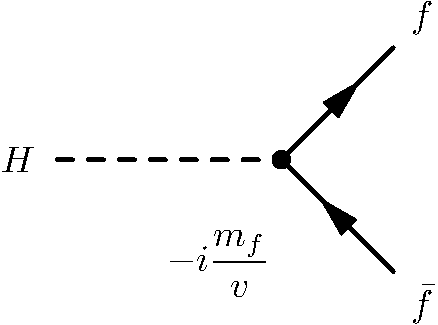
\includegraphics[height=3.5cm]{figures/FD_HFFterm.pdf}
\caption{ Feynman diagram for Hff interaction.}
\label{fig:fd_HFFterm}
\end{figure}





%%%%%%%%%%%%%%%%%%%%%%%%%%%%%%%%%%%%%%%%%%%%%%%%%%%%%%%%%%%%%%%%
\newpage
\section{Production and Decay of Higgs Boson}


\subsection{Production of Higgs Boson}

At LHC, the Standard Model Higgs boson is generated by 4 major processes, 
gluon-gluon fusion (\ggH), 
vector boson fusion (\qqH),
associated production with vector bosons (\qqVH) and 
associated production with heavy quarks(\ttH).
The corresponding Fenyman diagrams are shown in Figure~\ref{fig:FD_HiggsProduction}.
\begin{figure}[htp] 
\centering 
\begin{tabular}{c} 
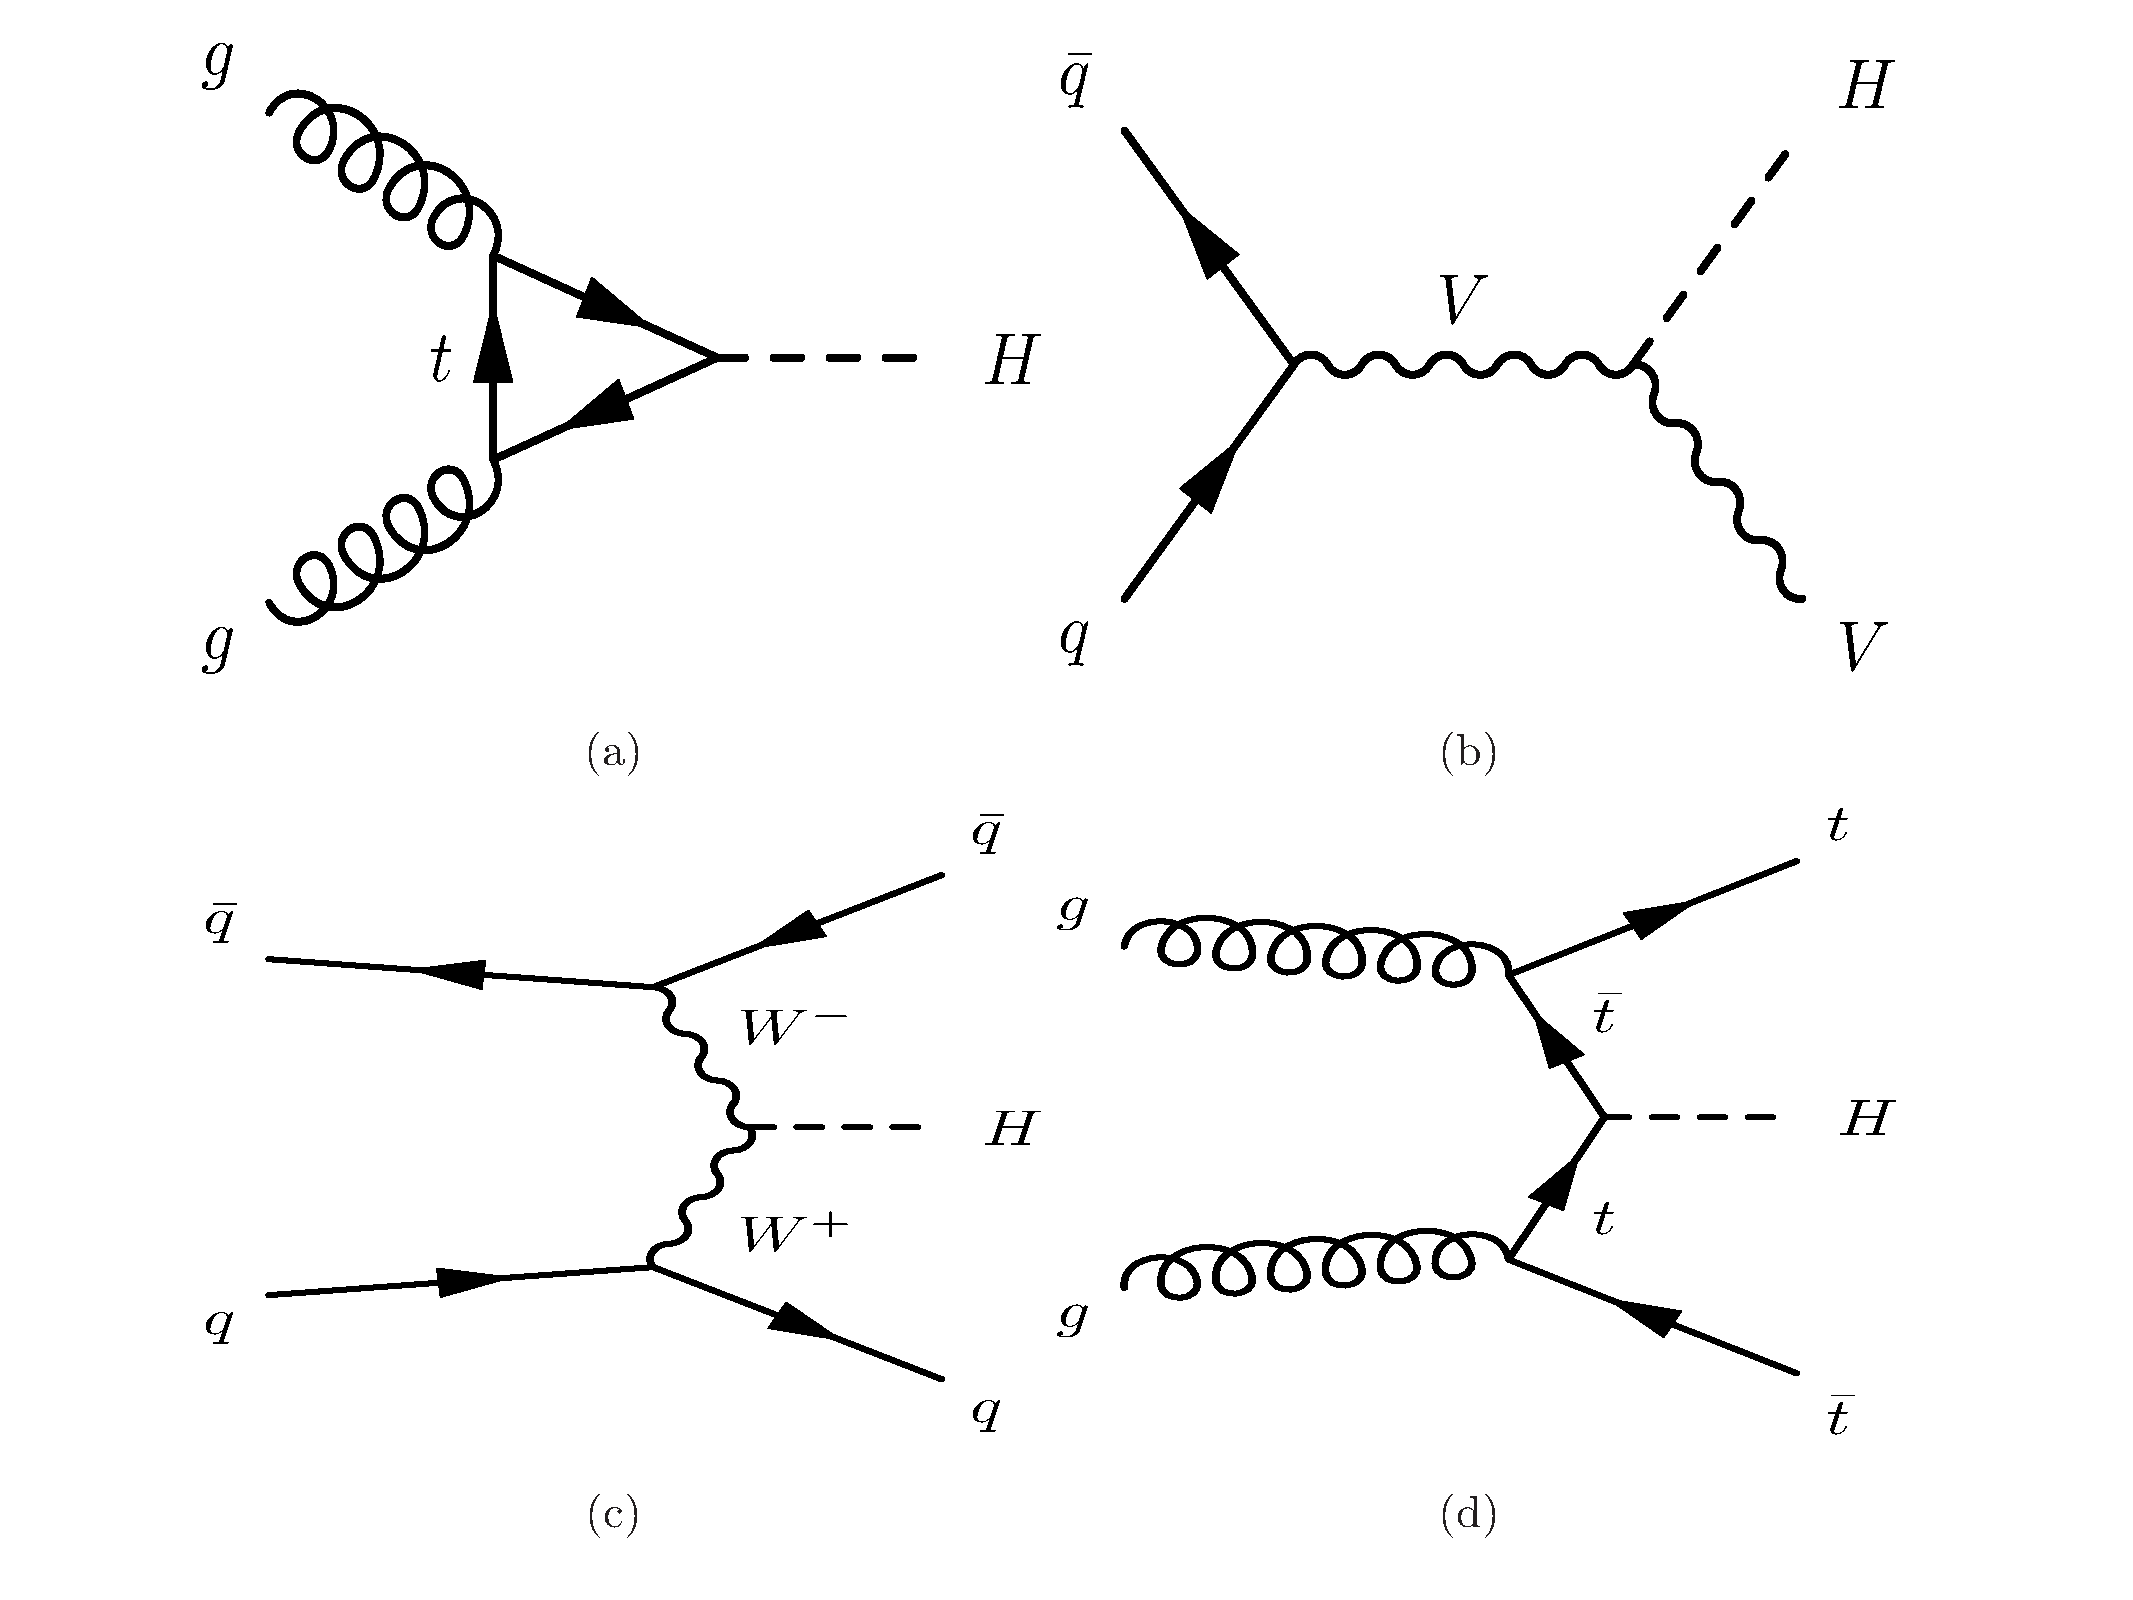
\includegraphics[width=0.9\textwidth]{figures/FD_HiggsProduction.pdf} 
\end{tabular} 
\caption{Feynman diagrams for SM Higgs production, (a) \ggH, (b) \qqVH, (c) \qqH\ and (d) \ttH.} 
\label{fig:FD_HiggsProduction} 
\end{figure} 
Since H does not couple to gluon in ggH process it is produced via a loop of 
heavy quarks, \textit{i.e.,} top and bottom quarks.
At LHC \ggH\ has the largest production rate because gluons have 
the largest probability to collide which is given by parton distribution function(PDF), 
and top quark has very large coupling to Higgs boson. 
\begin{figure*}[t]
\centering
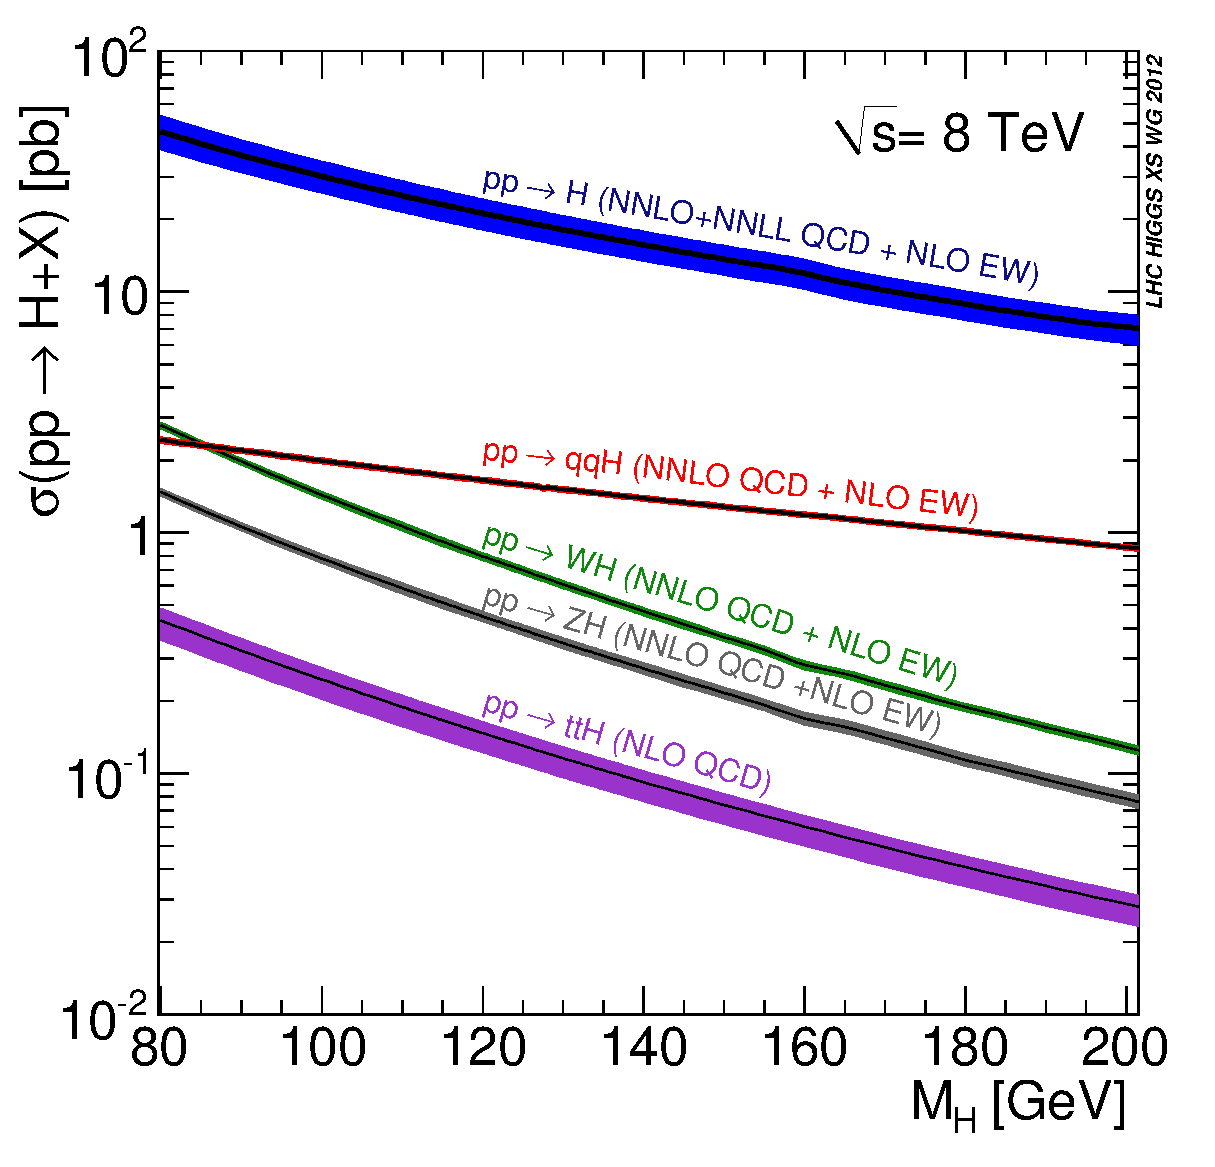
\includegraphics[width=0.8\textwidth]{figures/Higgs_XS_8TeV_LM200.eps}
\caption{ Standard model Higgs production cross sections 
as a function of \mHi\ at $\sqrt{s}=8~\TeV$ for each 
production mode. %\cite{Dittmaier:2012vm}. 
The \ggH\ and \qqH\ processes are 
calculated in complex-pole-scheme(CPS)~\cite{Goria:2011wa}, while other WH/ZH and ttH processes 
are calculated in zero-width-approximation(ZWA)~\cite{pilkuhn1967interactions}. }
% Ref is  https://twiki.cern.ch/twiki/bin/view/LHCPhysics/CERNYellowReportPageAt8TeV
\label{fig:Higgs_XS_8TeV_LM200}
\end{figure*}

At the hadron colliders the hadronic cross section($\sigma$) is calculated with 
parton-level cross-section ($\hat{\sigma}$) convoluted with PDF, 
\begin{eqnarray} 
\sigma (pp \rightarrow H+X) 
= 
\sum_{i,j} \int dx_1 dx_2 f_i(x_1) f_j(x_2) 
\hat{\sigma} \left( ij \rightarrow H+X \right)
\end{eqnarray} 
where i and j are colliding partons, 
$x_1$ and $x_2$ are the longitudinal momentum fractions carried by parton i and j. 
Each component in the equation is subject to the following uncertainties.
The partonic cross section is calculated at a given
renormalization scale($\mu_R$) and factorization scale($\mu_F$). 
Due to possible missing higher-order QCD radiative corrections,
the uncertainty is estimated by varying the scales around 
the central values. In the de Florian and Grazzini (dFG) 
calculation [ref], the central values are chosen to be $\mu_0 = \mHi$. 
The scales $\mu_R$ and $\mu_F$ are varied in the range 
%$\displaystyle \frac{1}{2}\mu_0 < \mu_F, \mu_R < 2\mu_0$ 
$\mu_0/2 < \mu_F, \mu_R < 2\mu_0$ 
%with a constraint $\displaystyle \frac{1}{2} < \frac{\mu_F}{\mu_R} < 2$. 
with a constraint $1/2 < \mu_F/\mu_R < 2$. 
PDF is obtained by fitting on data measured in deep-inelastic scattering, 
Drell-Yan, and jet production from a wide variety of different experiments. 
The accuracy on those data can introduce uncertainty on PDF calculation. 
In addition, strong coupling constant $\alpha_s$ is used in DGLAP 
evolution~\cite{Altarelli:1977zs,Dokshitzer:1977sg,Gribov:1972ri} 
to the higher $Q^2$ region. Thus, its uncertainty also contributes to 
the total cross section. There are other uncertainties due to 
EWK corrections, the different choice of top and bottom quark masses, 
and the use of large-$m_T$ method. But, the effect of these uncertainties to the 
hadronic cross section is less than a few percent \cite{Dittmaier:2012vm}
for \ggH.

Figure \ref{fig:Higgs_XS_8TeV_LM200} shows the hadronic cross sections 
as a function of \mHi\ for SM Higgs production and uncertainty 
in different production modes. The \ggH\ and \qqH\ cross sections 
are based on complex-pole-scheme (CPS), while VH and ttH ones 
are based on zero-width-approximation (ZWA). 
\begin{table}[htb]
\centering
\vspace{0.5cm} 
\caption{The highest order of QCD and EW calculations.}
\label{tab:Higgs_XS_8TeV_order}
\vspace{0.5cm} 
\begin{tabular}{c c c  }
\hline
process     & QCD   & EW \\
\hline \hline 
$ pp \rightarrow H$         & NNLO  & NLO \\
$ pp \rightarrow qqH$       & NNLO  & NLO \\
$ pp \rightarrow WH$        & NNLO  & NLO \\
$ pp \rightarrow ZH$        & NNLO  & NLO \\
$ pp \rightarrow ttH$       & NLO   &     \\
\hline 
\end{tabular}
\end{table}
The highest order of QCD and EW calculations are summarized in Table 
\ref{tab:Higgs_XS_8TeV_order}. The uncertainty is a linear combination 
of uncertainties from QCD scale variation and PDF+$\alpha_S$.
At $\mHi=125~\GeV$ \ggH\ contributes $\sim 87 \%$ to the total cross section.


%The PDF and parton-level cross section depend on the 
%renormalizaion scale $\mu_R$ because they contain ultraviolet divergences 
%to be subtacted through a renormalization procedure. [ref] 
%In addition PDF is calculated with a factorization scale $\mu_F$.

%%%
\newpage
\subsection{Decay of Higgs Boson}
\label{sec:decayHiggs}

Figure~\ref{fig:fd_HVterm} shows that the Higgs boson can 
couple to a pair of weak bosons. Thus, Higgs can directly decay into $W^+W^-$ and $ZZ$.
Depending on \mHi, one or two of the bosons can be off-shell. 
As shown in~\cite{Djouadi20081}, at $\mHi>2m_W$ both bosons 
tend to be on-shell, and at $110<\mHi<2m_W$ one of them is on-shell 
while the other is off-shell. Below 110~\GeV\ there is a sizable contribution 
from the case where both bosons are off-shell, but this is not relevant 
to this analysis. Thus, we discuss two cases where both of them are on-shell$(VV)$, 
and one is on-shell and the other is off-shell$(VV^*)$. 

%
\subsubsection{Both bosons are on shell : $H \rightarrow VV$}
When both bosons are on-shell($ H \rightarrow VV$), 
the decay width at tree-level is given by~\cite{PhysRevD.49.79}
\begin{eqnarray} 
\Gamma \left( H \rightarrow VV \right) 
= 
\frac{\gf \mHi^3}{16\sqrt{2\pi}} \delta_V \sqrt{1-4\epsilon^2} 
\left( 1 - 4\epsilon^2 + 12\epsilon^4 \right)
\end{eqnarray} 
where $\displaystyle \epsilon = \frac{m_V}{\mHi}$ and $\delta_W=2$ and $\delta_Z=1$.
At high \mHi, the decay width to WW is reduced to 
\begin{eqnarray} 
\Gamma \left( H \rightarrow WW \right)
&\rightarrow&
\frac{\gf \mHi^3}{16\sqrt{2\pi}} \times 2 \\
&=&  
2 \frac{ 1.16637 \times 10^{-5}~\GeV^{-2} \mHi^3}{16\sqrt{2\pi}} \\
&\approx&
0.33 \mHi \times \frac{\mHi^2}{\TeV^2} (\TeV).   
\end{eqnarray} 
For example, at $\mHi=1~\TeV$, decay width for WW is 0.33 \TeV.
Practically, it is hard to claim a Higgs resonance at high mass regions.  

The ratio of longitudinal polarization is given by \cite{PhysRevD.49.79}
\begin{eqnarray} 
R_L 
= 
\frac{\Gamma_L}{\Gamma_T + \Gamma_L}    
= 
\frac{1 - 4\epsilon^2 + 4\epsilon^4}{1 - 4\epsilon^2 + 12\epsilon^4} 
\xrightarrow{\epsilon \rightarrow 0}\ 1.
\end{eqnarray} 
Thus, vector bosons are longitudinally polarized at high \mHi\ ($\epsilon \rightarrow 0$). 
%At the production threshold, $\displaystyle \mHi = 2m_V \rightarrow \epsilon = \frac{1}{2}$, 
At the production threshold, $\displaystyle \mHi = 2m_V$ ($\epsilon = 1/2$), 
$R_L$ is 1/3 which means that the longitudinal and the transverse polarizations are populated 
with a ratio of 1:2. This is shown in the Figure~\ref{fig:HVV_polarization_ratio}.

%
\subsubsection{One boson is on-shell and other is off-shell : 
               $H \rightarrow VV^* \rightarrow Vf\bar{f}$}
When one boson is on-shell and the other is off-shell
($ H \rightarrow VV^* \rightarrow Vf\bar{f}$), % where $f$ does not include top quark),
the decay width at tree-level is given by~\cite{PhysRevD.49.79}
\begin{eqnarray} 
\Gamma \left( H \rightarrow VV^* \right) 
=
\frac{3\gf^2 m_V^4}{16\pi^3} \mHi \delta_V' R(\epsilon)
\end{eqnarray} 
where $\delta_W'=1$, $\displaystyle \delta_Z'=\frac{7}{12}-\frac{10}{9}\sin^2\theta_W 
+ \frac{40}{9}\sin^4\theta_W$ and 
\begin{eqnarray}   
\begin{array}{ccc} \multicolumn{2}{c}{\displaystyle 
R(\epsilon) = \frac{3(1-8\epsilon^2+20\epsilon^4)}{(4\epsilon^2-1)^{1/2}} 
                \arccos \left( \frac{3\epsilon^2-1}{2\epsilon^3} \right)  
} & \\ & \multicolumn{2}{c}{\hspace{1.5cm} \displaystyle
- (1-\epsilon^2)\left( \frac{47}{2}\epsilon^2 - \frac{13}{2} + \frac{1}{\epsilon^2} \right)  
- 3(1-6\epsilon^2+4\epsilon^4) \ln \epsilon.
} \end{array}      
\end{eqnarray} 

The ratio of longitudinal polarization is given \cite{PhysRevD.49.79} by 
\begin{eqnarray} 
R_L 
=
\frac{\Gamma_L}{\Gamma_T + \Gamma_L}    
= 
\frac{R_L(\epsilon)}{R(\epsilon)}  
\end{eqnarray} 
where $R_L$ is \cite{PhysRevD.49.79} 
\begin{eqnarray} 
\begin{array}{ccc} \multicolumn{2}{c}{\displaystyle 
R_L(\epsilon) = \frac{3(1-16\epsilon^2+20\epsilon^4)}{(4\epsilon^2-1)^{1/2}} 
                \arccos \left( \frac{3\epsilon^2-1}{2\epsilon^3} \right)  
} & \\ & \multicolumn{2}{c}{\hspace{1.5cm} \displaystyle
- (1-\epsilon^2)\left( \frac{15}{2}\epsilon^2 - \frac{13}{2} + \frac{1}{\epsilon^2} \right)  
- (3-10\epsilon^2+4\epsilon^4) \ln \epsilon.
} \end{array}      
\end{eqnarray} 
%
\begin{figure*}[t]
\centering
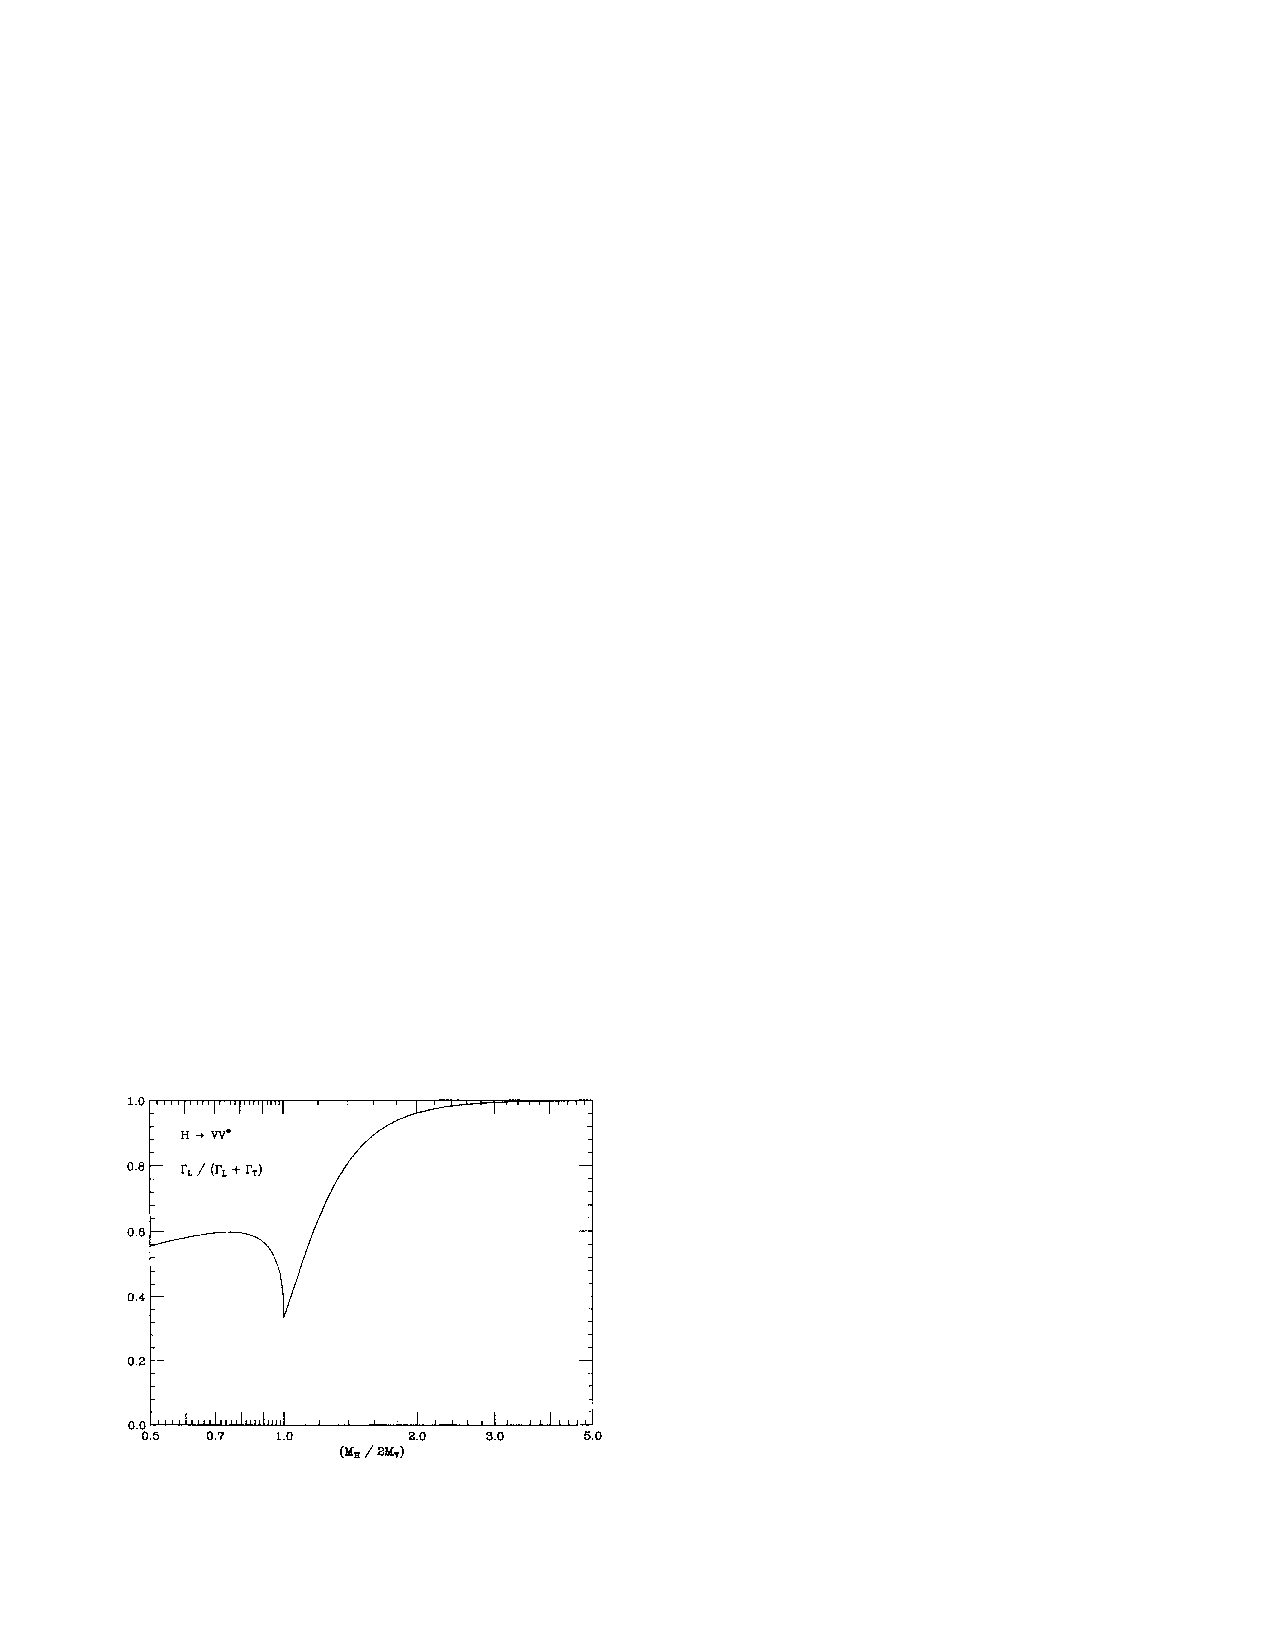
\includegraphics[width=0.6\textwidth]{figures/HVV_polarization_ratio.pdf}
\caption{The ratio of longitudinal polarization of vector bosons 
as a function of $\frac{\mHi}{2m_V}$ \cite{PhysRevD.49.79} }
\label{fig:HVV_polarization_ratio}
\end{figure*}
Figure~\ref{fig:HVV_polarization_ratio} shows the fraction of longitudinal $VV(*)$ decays 
%as a function of $\displaystyle \frac{\mHi}{2m_V}$
as a function of $\mHi/2m_V$(=$\displaystyle \frac{\epsilon}{2}$). 
As discussed in the VV decay, the fraction goes to 1 at high \mHi\ and 
to 1/3 at the production threshold, $\mHi = 2m_V$.
Below the threshold, the fraction of longitudinal polarization 
increases up to 0.6 at $\mHi/2m_V \approx 0.8 \rightarrow \mHi \approx 130~\GeV$,
and decreases slightly as \mHi\ becomes smaller. 
As the fraction of decay to longitudinally polarized bosons depends on \mHi, 
and the event kinematics depends on the fraction as well, 
it is important to optimize analysis for a given \mHi\ to maximize sensitivity. 
\\ 

Figure \ref{fig:YRHXS2_BR_Fig1} shows the branching ratios of Standard 
Model Higgs boson(left) and its total decay width(right). The partial widths of each 
decay mode are calculated with the next-leading-order(NLO) QCD 
and electron corrections, and all interferences at LO and NLO are 
taken into account~\cite{Dittmaier:1318996}. The band on the left plots 
shows the uncertainty due to missing higher order terms. 
%
\begin{figure*}[htp]
\centering
\subfigure[Branching ratios]{
\centering
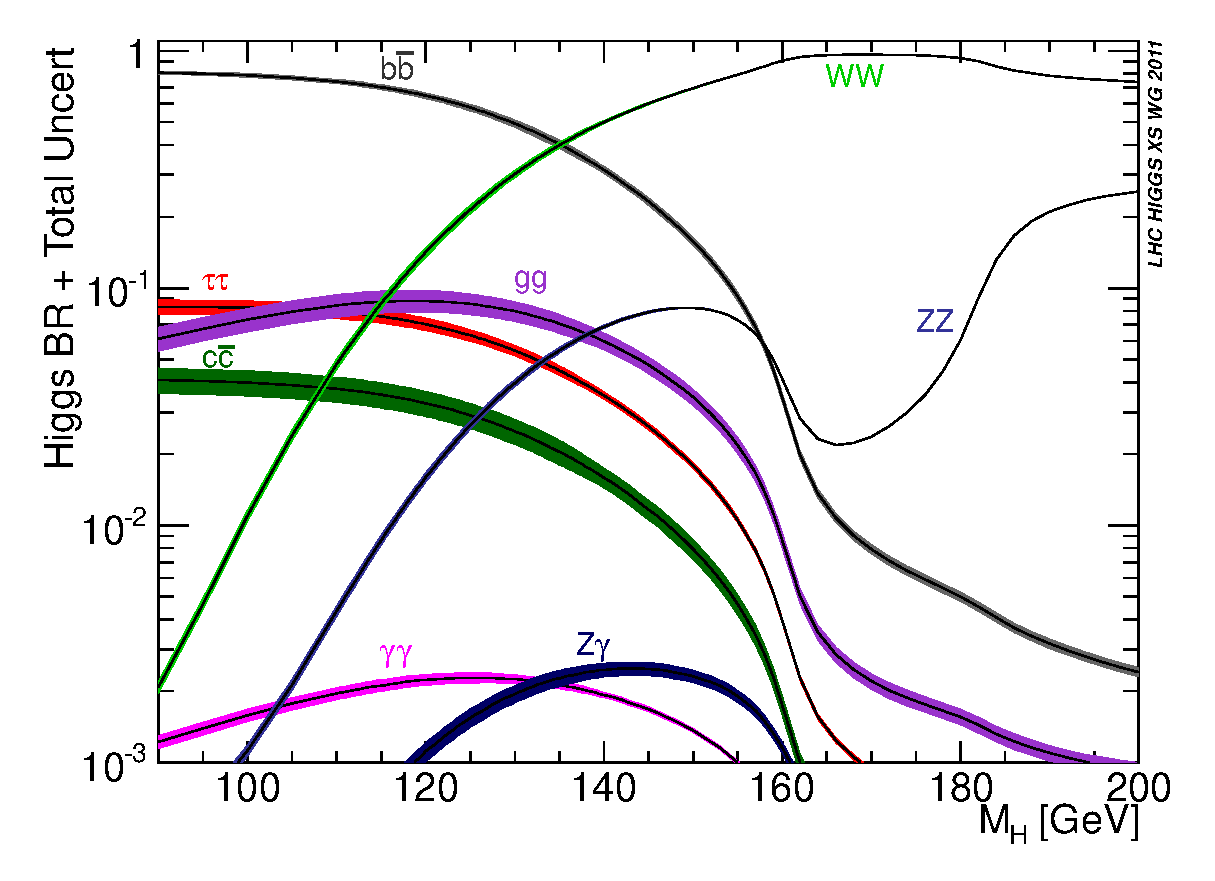
\includegraphics[width=0.8\textwidth]{figures/YRHXS2_BR_Fig1.eps}  
}
\subfigure[Total width]{
\centering
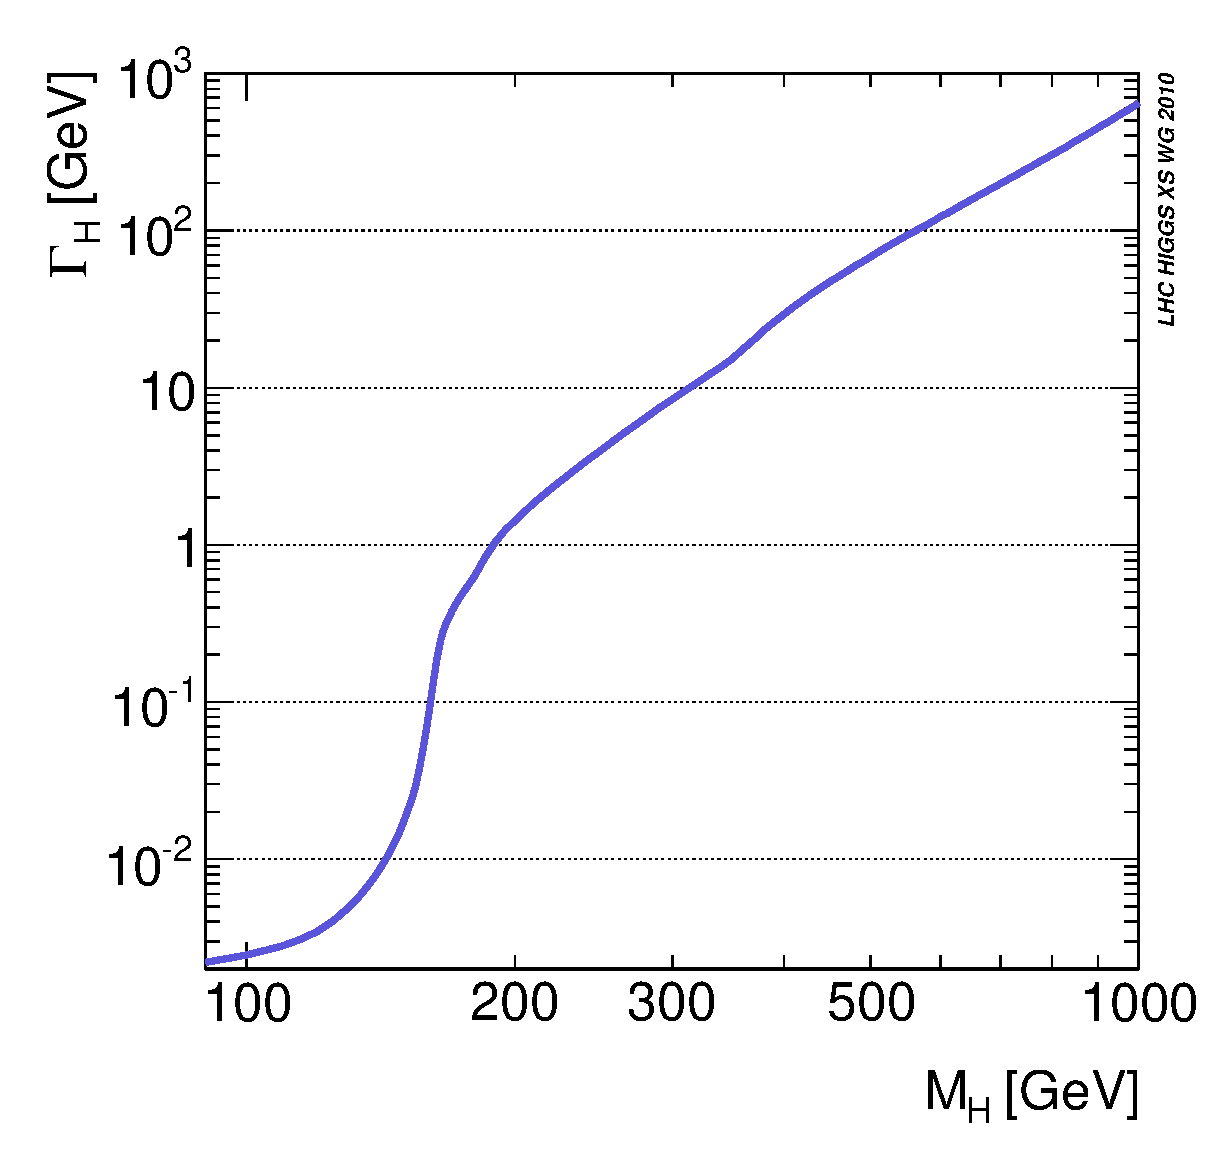
\includegraphics[width=0.7\textwidth]{figures/YRHXS_BR_fig2}
}
\caption{Standard Model Higgs boson decay branching ratios at low \mHi 
and the total width.}
\label{fig:YRHXS2_BR_Fig1}
\end{figure*}


%%%%%%%%%%%%%%%%%%%%%%%%%%%%%%%%%%%%%%%%%%%%%%%%%%%%%%%%%%%%%%%%
\newpage
\section{Limits on Higgs Boson Mass} 


The Higgs mass is constrained by various theoretical limits 
and experimental measurements. This section discusses theoretical 
limits by perturbative unitarity, triviality and stability, 
and fine tuning. Then it discusses the experimental limits 
from indirect and direct measurements as of 2011. 


\subsection{Theoretical Limits} 

\subsubsection{Perturbative Unitarity : $W_L^+W_L^- \rightarrow W_L^+W_L^-$}

The cross section of longitudinal vector boson scattering, $V_LV_L \to V_LV_L$, 
increases as the energy increases, and it eventually violates unitarity, 
\textit{i.e.}, probability for this process to happen is larger than unity. 

\begin{figure*}[t]
\centering
\subfigure[]{
\centering
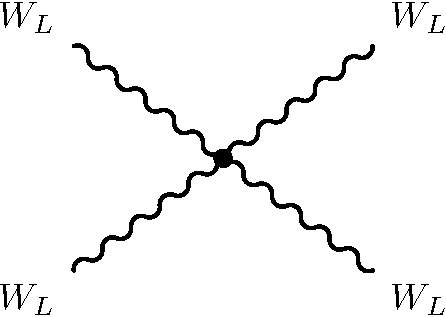
\includegraphics[width=0.25\textwidth]{figures/WWscat0.pdf} 
}
\hspace{0.5cm}
\subfigure[]{
\centering
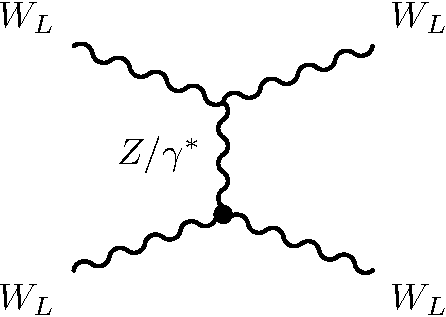
\includegraphics[width=0.25\textwidth]{figures/WWscat_tchZ.pdf}
}
\hspace{0.5cm}
\subfigure[]{
\centering
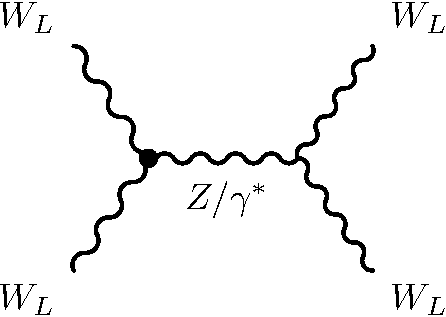
\includegraphics[width=0.25\textwidth]{figures/WWscat_schZ.pdf}
}
\\
\vspace{0.5cm}
\subfigure[]{
\centering
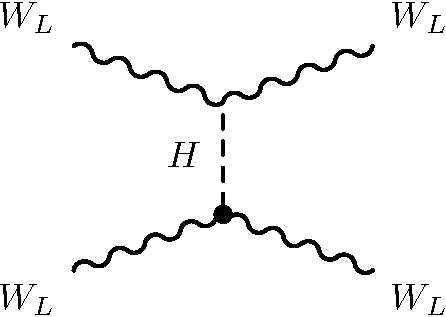
\includegraphics[width=0.25\textwidth]{figures/WWscat_tchH.pdf}
}
\hspace{0.5cm}
\subfigure[]{
\centering
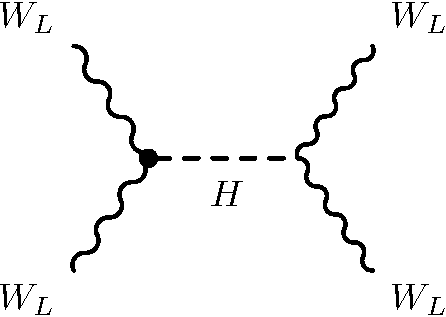
\includegraphics[width=0.25\textwidth]{figures/WWscat_schH.pdf}
}
\caption{Feynman diagrams for $W_L^+W_L^- \to W_L^+W_L^-$ scattering.} 
\label{fig:FD_unitary}
\end{figure*}
Figure~\ref{fig:FD_unitary} shows Feynman diagrams for $W_L^+W_L^- \to W_L^+W_L^-$. 
There are 4-point interaction, and t-channel and s-channel interactions mediated 
by $Z/\gamma^*$ or Higgs boson.
In the high energy limit $s \gg \mW^2$, the scattering amplitude becomes \cite{Djouadi20081} 
\begin{eqnarray} 
\label{eq:WWscat}
\mathcal{A}\left( W_L^+W_L^- \to W_L^+W_L^- \right) 
\sim 
- \frac{1}{v^2}  \left( -s - t + \frac{s^2}{s - \mHi^2} + \frac{t^2}{t - \mHi^2} \right). 
\end{eqnarray} 
%\textcolor{red}{What does the point diagram correspond to in this equation?
%look at Users/jaehyeok/Research/cms/References/Theory/0910.4182v4.pdf}  
According to the Electroweak Equivalence Theorem~\cite{He:1994br},  
at very high energy the longitudinal vector bosons can be replaced by 
their associated Goldstone bosons. Thus, the scattering amplitude can be written 
using Goldstone bosons ($w^\pm$)
\begin{eqnarray} 
\mathcal{A}\left( w^+w^- \to w^+w^- \right) 
= 
- \frac{\mHi^2}{v^2}  \left( 2 + \frac{\mHi^2}{s - \mHi^2} + \frac{\mHi^2}{t - \mHi^2} \right). 
\end{eqnarray} 
An scattering amplitude can be decomposed into partial waves $a_l$
\begin{eqnarray} 
\mathcal{A} = 16 \pi \sum_{i=0}^\infty 
              \left( 2l+1 \right) P_l \left( \cos \theta \right) a_l
\end{eqnarray} 
where $P_l$ is the Legendre polynomials and $\theta$ is the scattering angle.
For the cross section of $2 \to 2$ processes, we have the 
following identity on the cross section ($\sigma$) by Optical theorem \cite{optical}
\begin{eqnarray} 
\sigma 
= \frac{16 \pi}{s} \sum_{i=0}^\infty  \left( 2l+1 \right) \left| a_l \right|^2 
= \frac{1}{s} Im \left[ \mathcal{A} \left(\theta = 0 \right)  \right]
\end{eqnarray} 
which gives the unitary condition, 
\begin{eqnarray} 
\left| a_l \right|^2 = Im \left( a_l \right) 
\quad &\Rightarrow& \quad  
Re\left( a_l \right)^2 
+ \left[ Im\left( a_l \right)  - \frac{1}{2} \right]^2 
= \left( \frac{1}{2} \right)^2 \\
\label{eq:unitaryWW}
\quad &\Rightarrow& \quad 
\left| Re \left( a_l \right) \right| < \frac{1}{2}.   
\end{eqnarray} 
Then, the $l=0$ amplitude in the limit of $ s \gg \mHi^2$ becomes  
\begin{eqnarray} 
a_0\left( w^+w^- \to w^+w^- \right)  
&=&  
- \frac{\mHi^2}{16\pi v^2}  
\left[ 2 + \frac{\mHi^2}{s - \mHi^2} 
       - \frac{\mHi^2}{s} \log \left( 1 + \frac{s}{\mHi^2} \right) \right]  \\
&\rightarrow&
- \frac{\mHi^2}{8\pi v^2} 
\end{eqnarray} 
The unitary condition (equation (\ref{eq:unitaryWW})) gives upper bound on \mHi, 
\begin{eqnarray} 
\left| Re \left( a_0 \right) \right| 
&=&  \frac{\mHi^2}{8\pi v^2} < \frac{1}{2} \\ 
&\Rightarrow& 
\mHi < 2 \sqrt{\pi} v \simeq 870~\GeV. 
\end{eqnarray} 
Including other scattering channels, 
\begin{eqnarray} 
Z_LZ_L, \,\,\, HH, \,\,\, Z_LH, \,\,\, W_L^+H, \,\,\, W^+_LZ_L 
\end{eqnarray} 
the constraint on \mHi\ becomes tighter as~\cite{Djouadi20081}, 
\begin{eqnarray} 
\label{eq:unitaryAll}
\mHi < 710~\GeV.
\end{eqnarray}
This means that in the standard model unitariry will be violated if $\mHi>710~\GeV$
unless there is a new physics that cures this problem. 

So far we calculated only tree-level terms, so we can expect that adding 
higher order terms can solve this problem. But, including higher order 
terms does not guarantee that the unitary will be restored because 
in the high \mHi\ regime coupling to Higgs is too large and perturbative 
calculation breaks down. Thus, the mass bound given in equation~(\ref{eq:unitaryAll})  
can be considered the \mHi~regime where perturbative calculation is reliable 
in all $s$.

\subsubsection{Triviality and Stability bounds}
% Triviality 
\begin{figure*}[t]
\centering
\subfigure[]{
\centering
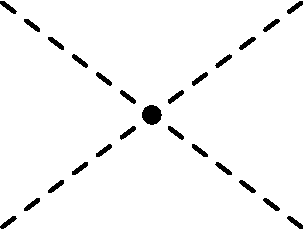
\includegraphics[width=0.2\textwidth]{figures/FD_HHHHtree.pdf} 
}
\hspace{0.3cm}
\subfigure[]{
\centering
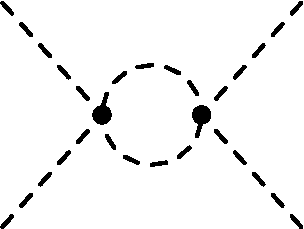
\includegraphics[width=0.2\textwidth]{figures/FD_HHHH1loop1.pdf}
} \hspace{0.3cm}
\subfigure[]{
\centering
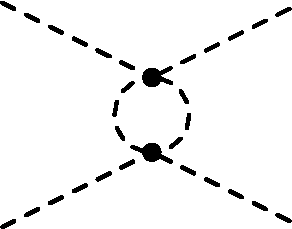
\includegraphics[width=0.2\textwidth]{figures/FD_HHHH1loop2.pdf}
}
\hspace{0.3cm}
\subfigure[]{
\centering 
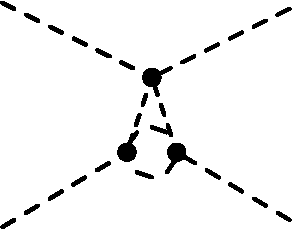
\includegraphics[width=0.2\textwidth]{figures/FD_HHHH1loop3.pdf} } 
\caption{Feynman diagrams for Higgs boson quartic interaction. Left is tree level and 
the right three are one-loop correction by Higgs boson itself.} 
\label{fig:FD_triviality} 
\end{figure*} 
The variation of the Higgs quartic coupling $\lambda$ is described by 
Renormalization Group Equation (RGE). 
When we consider one-loop radiation corrections by Higgs boson itself 
to $\lambda$ as shown in Figure~\ref{fig:FD_triviality}, 
the corresponding RGE is given by \cite{Djouadi20081} 
\begin{eqnarray} 
\frac{d}{dQ^2} \lambda (Q^2) 
= 
\frac{3}{4\pi^2} \lambda^2(Q^2) + \textrm{higher orders} 
\end{eqnarray} 
The solution to this equation is given by 
\begin{eqnarray} 
\displaystyle  \lambda(Q^2) = \frac{\lambda(v^2)} {\left[\displaystyle   1 - \frac{3}{4\pi^2} \lambda(v^2) \log{\frac{Q^2}{v^2}}\right] } 
\end{eqnarray} 
where the EWSB scale is used as a reference energy point, $Q_0 = v$. 

If the energy is much smaller than the EWSB scale, $Q^2\ll v^2$, 
the quadratic coupling goes to 0, and the theory is called 
``trivial", which means that there is no interaction. 
On the other hand, if the energy is much larger than the EWSB scale, $Q^2\gg v^2$,
as Q increases the coupling will be infinite at a certain energy scale, $\Lambda_{cut}$. 
Using $\lambda = \mHi^2/2v^2$ and the definition of $\lambda$ that it is positive, 
we have the following equation for denominator,
\begin{eqnarray} 
1 > \frac{3}{4\pi^2} \frac{\mHi^2}{2v^2} \log{\frac{\Lambda_{cut}^2}{v^2}} 
\qquad \Rightarrow  \qquad 
\mHi^2 > \frac{8\pi^2v^2}{\log{\displaystyle  \frac{\Lambda_{cut}^2}{v^2}}},
\end{eqnarray} 
which gives a scale-dependent bound on \mHi. Imposing $\Lambda_{cut} = \mHi$ 
which means that the theory is not reliable, \textit{i.e.}, valid scale of the theory is same 
as the mass of a particle, the bound on the Higgs mass is $\mHi < 640~\GeV$. 
This result is consistent with the limit from unitarity constraint. 
\\

% Stability 
In the previous discussion, only one-loop correction by Higgs itself is considered.
This is a proper approximation when $\lambda$ is large, but
when $\lambda$ is small, we need to consider the contributions from fermions 
and vector bosons. Since, the strength of interaction with Higgs boson is proportional 
to the particle mass, we consider only heavy particles, vector bosons and top quarks.   

In the limit of small Higgs quartic couplings, $\lambda \ll \lambda_t, g_1, g_2$ 
where $\lambda_t$ is the top Yukawa coupling given by $\sqrt{2} \mt / v$, the RGE is 
given by \cite{Djouadi20081}
\begin{eqnarray}
\label{eq:stability_ddlogQ2}
\frac{d}{dQ^2} \lambda (Q^2)  
\simeq
\frac{1}{16\pi^2}  
\left[ -12 \frac{\mt^4}{v^4} + \frac{3}{16} \left(2g_2^4 + \left(g_2^2+g_1^2\right)^2 \right)   \right].
\end{eqnarray} 
Taking EWSB scale as the reference point, the solution to equation~(\ref{eq:stability_ddlogQ2}) is  
\begin{eqnarray} 
\lambda\left(Q^2\right) 
= 
\lambda\left(v^2\right)  
+ 
\frac{1}{16\pi^2}  \left[ -12 \frac{\mt^4}{v^4} 
                          + \frac{3}{16} \left(2g_2^4 + \left(g_2^2+g_1^2\right)^2 \right) \right]
                    \log \frac{Q^2}{v^2}.
\end{eqnarray} 
As $\lambda(v^2)$ becomes small, the coupling can go negative, and the vacuum becomes unstable.   
Thus, in order to maintain the stability of vacuum, $\lambda\left(Q^2\right)$ should be 
positive. This requirement gives
\begin{eqnarray} 
\mHi^2 
&>&
\frac{v^2}{8\pi^2}  \left[ -12 \frac{\mt^4}{v^4} 
                          + \frac{3}{16} \left(2g_2^4 + \left(g_2^2+g_1^2\right)^2 \right) \right]
                    \log \frac{\Lambda_{cut}^2}{v^2} 
\end{eqnarray} 
%
\begin{figure*}[t]
\centering
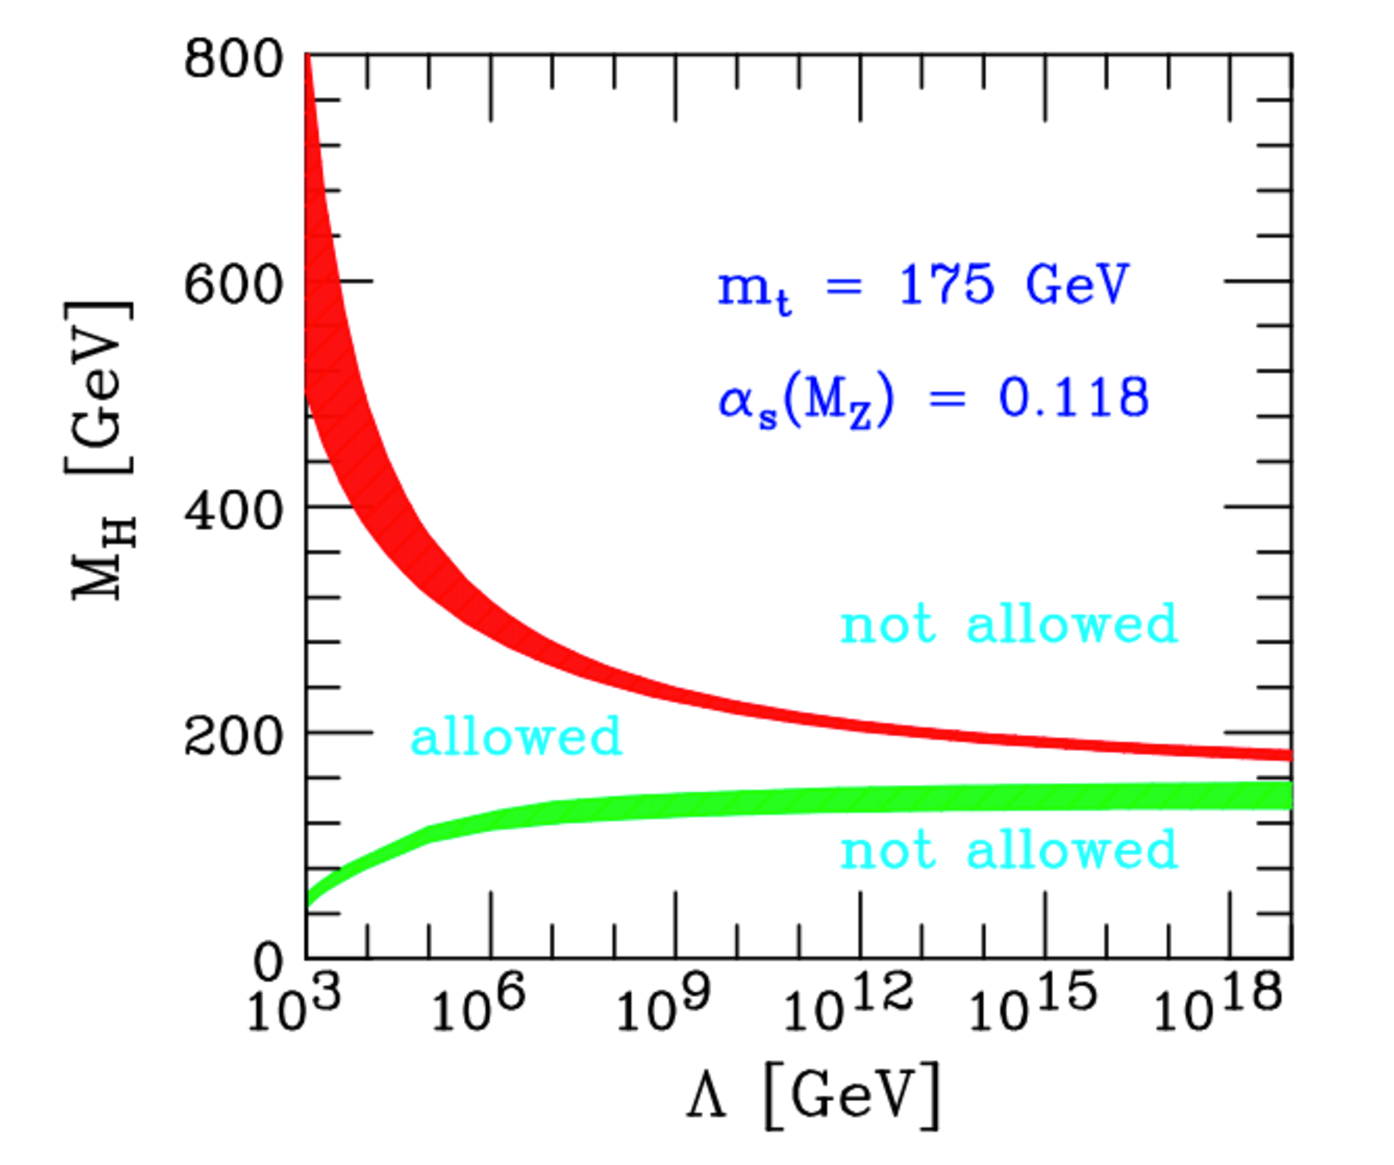
\includegraphics[width=0.8\textwidth]{figures/trivial_vacstab.pdf}
\caption{ Upper and lower bound of \mHi\ as a function of $\Lambda_{cut}$.
}
\label{fig:trivial_vacstab}
\end{figure*}
\\

So far the higher order contributions were taken up to 1-loop corrections. 
There are calculations up to 2-loops and Figure~\ref{fig:trivial_vacstab} 
shows lower bound (vacuum stability) and upper bound (triviality) of \mHi\ 
as a function of cutoff scale, $\Lambda_{cut}$~\cite{Djouadi20081}.

%
\subsubsection{Fine tuning}
The 1-loop radiative corrections to \mHi\ when only W/Z/H and top contributions 
are considered are given by~\cite{Djouadi20081}
\begin{eqnarray} 
\mHi^2 
= 
\left( \mHi^0 \right)^2 + \frac{3 \Lambda^2}{8\pi^2v^2} 
\left[ \mHi^2 + 2\mW^2 + \mZ^2- 4 \mt^2 \right] 
\end{eqnarray} 
where $\mHi^0$ is the fundamental parameter of SM, $\Lambda$ is the 
cutoff scale, and $\mW, \mZ, \mt$ are W, Z, top mass, respectively. 
Therefore, unless $\Lambda$ is in the same scale of 
EWSB($100~\GeV - 1~\TeV$), there should be an incredible fine-tuning between 
$\mHi^0$ and the radiative correction to have \mHi\ in the EWSB scale.  

For a quantitative discussion, we first need to define what fine-tuning means. 
Fine-tuning is defined as the sensitivity of the weak scale to
the cutoff, $\left| \delta \mW^2(\Lambda) / \mW^2 \right|$, where $\delta \mW^2$ is the 
difference between the tree and loop values, with all other quantities held fixed 
\cite{Kolda:2000wi}.
So, the metric, $\mathcal{F}$, is  
\begin{eqnarray} 
\mathcal{F}
= \left| \frac{\delta \mW^2}{\mW^2} \right|
= \left| \frac{\delta v^2}{v^2} \right|
= \left| \frac{\delta \mu^2}{\mu^2} \right|
= \left| \frac{\delta \mHi^2}{\mHi^2} \right|
= \frac{2\Lambda^2}{\mHi^2} \left| \sum_{n} 
  \log^2\left( \frac{\Lambda}{\mHi} \right) \right| 
\end{eqnarray} 
and $\mathcal{F} \le 1$ represents that there is no fine-tuning. 

\begin{figure*}[t]
\centering
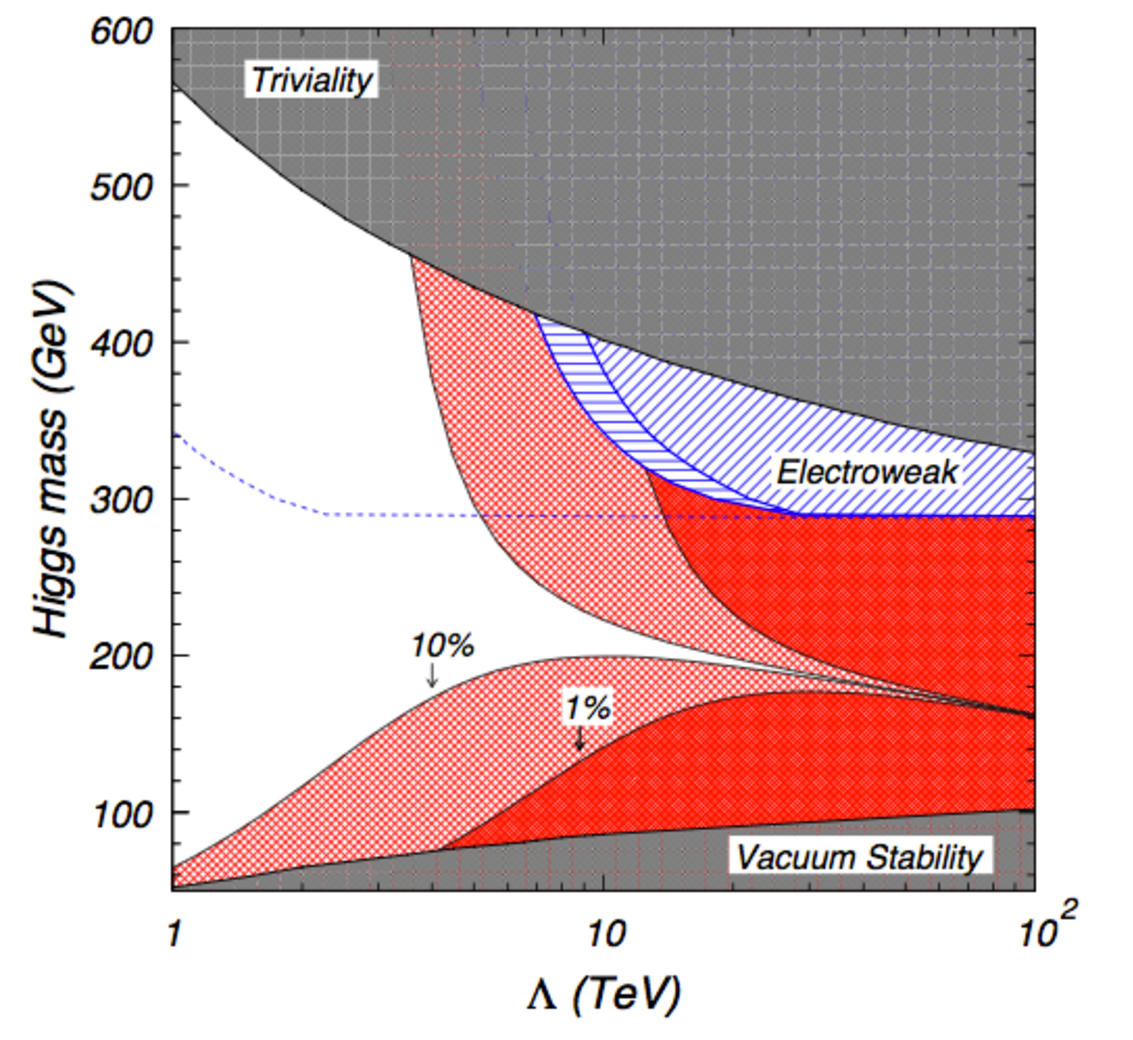
\includegraphics[width=0.8\textwidth]{figures/finetuning.pdf}
\caption{Constraint contour from fine tuning, vacuum stability, and triviality}.
\label{fig:finetuning}
\end{figure*}

The Figure~\ref{fig:finetuning} \cite{Kolda:2000wi} shows two regions in $[\Lambda,\mHi]$ plane
where $\Lambda$ is the cutoff scale; 
$\mathcal{F}>10$ in light-hatching (labeled as $10~\%$)
and $\mathcal{F}>100$ in thick-hatching (labeled as $1~\%$).  
In case of light Higgs scenario, the fine-tuning is required even at the low energy scale. 
For example, at \mHi=130 \GeV\ the fine-tuning of $\mathcal{F}>10$ requires 
$\Lambda<2.3~\TeV$. This means that new physics should exist in the regime where 
LHC experiments can probe.

%%
\newpage
\subsection{Experimental Limits} 

%
\subsubsection{Indirect search} 

There are electroweak measurements sensitive to \mHi. 
\begin{figure*}[t]
\centering
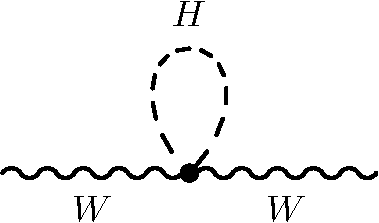
\includegraphics[width=0.3\textwidth]{figures/FD_Wmass_Hloop.pdf}
\caption{Feynman diagram for 1 loop correction by Higgs boson to the W propagator.}.
\label{fig:FD_Wmass_Hloop}
\end{figure*}
For example, the mass of W boson has one-loop correction of Higgs boson 
as shown in Figure~\ref{fig:FD_Wmass_Hloop}. Its contribution to the W mass 
is parametrized by $\Delta r$ in the following equation~\cite{Djouadi20081} % page 41
\begin{eqnarray} 
\mW^2 
= 
\frac{\pi\alpha}{\sqrt{2} \gf} 
\frac{1}{\left( 1 - \frac{\mW^2}{\mZ^2} \right)} 
\left( 1 + \Delta r \right),
\end{eqnarray} 
and the correction is 
\begin{eqnarray}
\Delta r \simeq 
\frac{\gf \mW^2}{8 \sqrt{2} \pi^2} \frac{11}{3} 
\left( \log \frac{\mHi^2}{\mW^2} - \frac{5}{6} \right)
\end{eqnarray} 
which is dependent on \mHi\ logarithmically. Thus, by measuring other quantities 
in the equation, we can constrain \mHi\ up to the uncertainties to the measured 
quantities. Going one step further, we can use more variables, not only \mW, 
and put them into a statistical fit \cite{LEP-2}. A simultaneous fit is done to
$\Delta \alpha_{had}^{(5)}(\mZ^2)$, $\alpha_S(\mZ^2)$,  
\mZ, \mt, and  $\log_{10} \left( \mHi \right)$
on the data collected by LEP-I/II, SLD, and Tevatron \cite{LEP-2}.  
\begin{figure*}[t]
\centering
%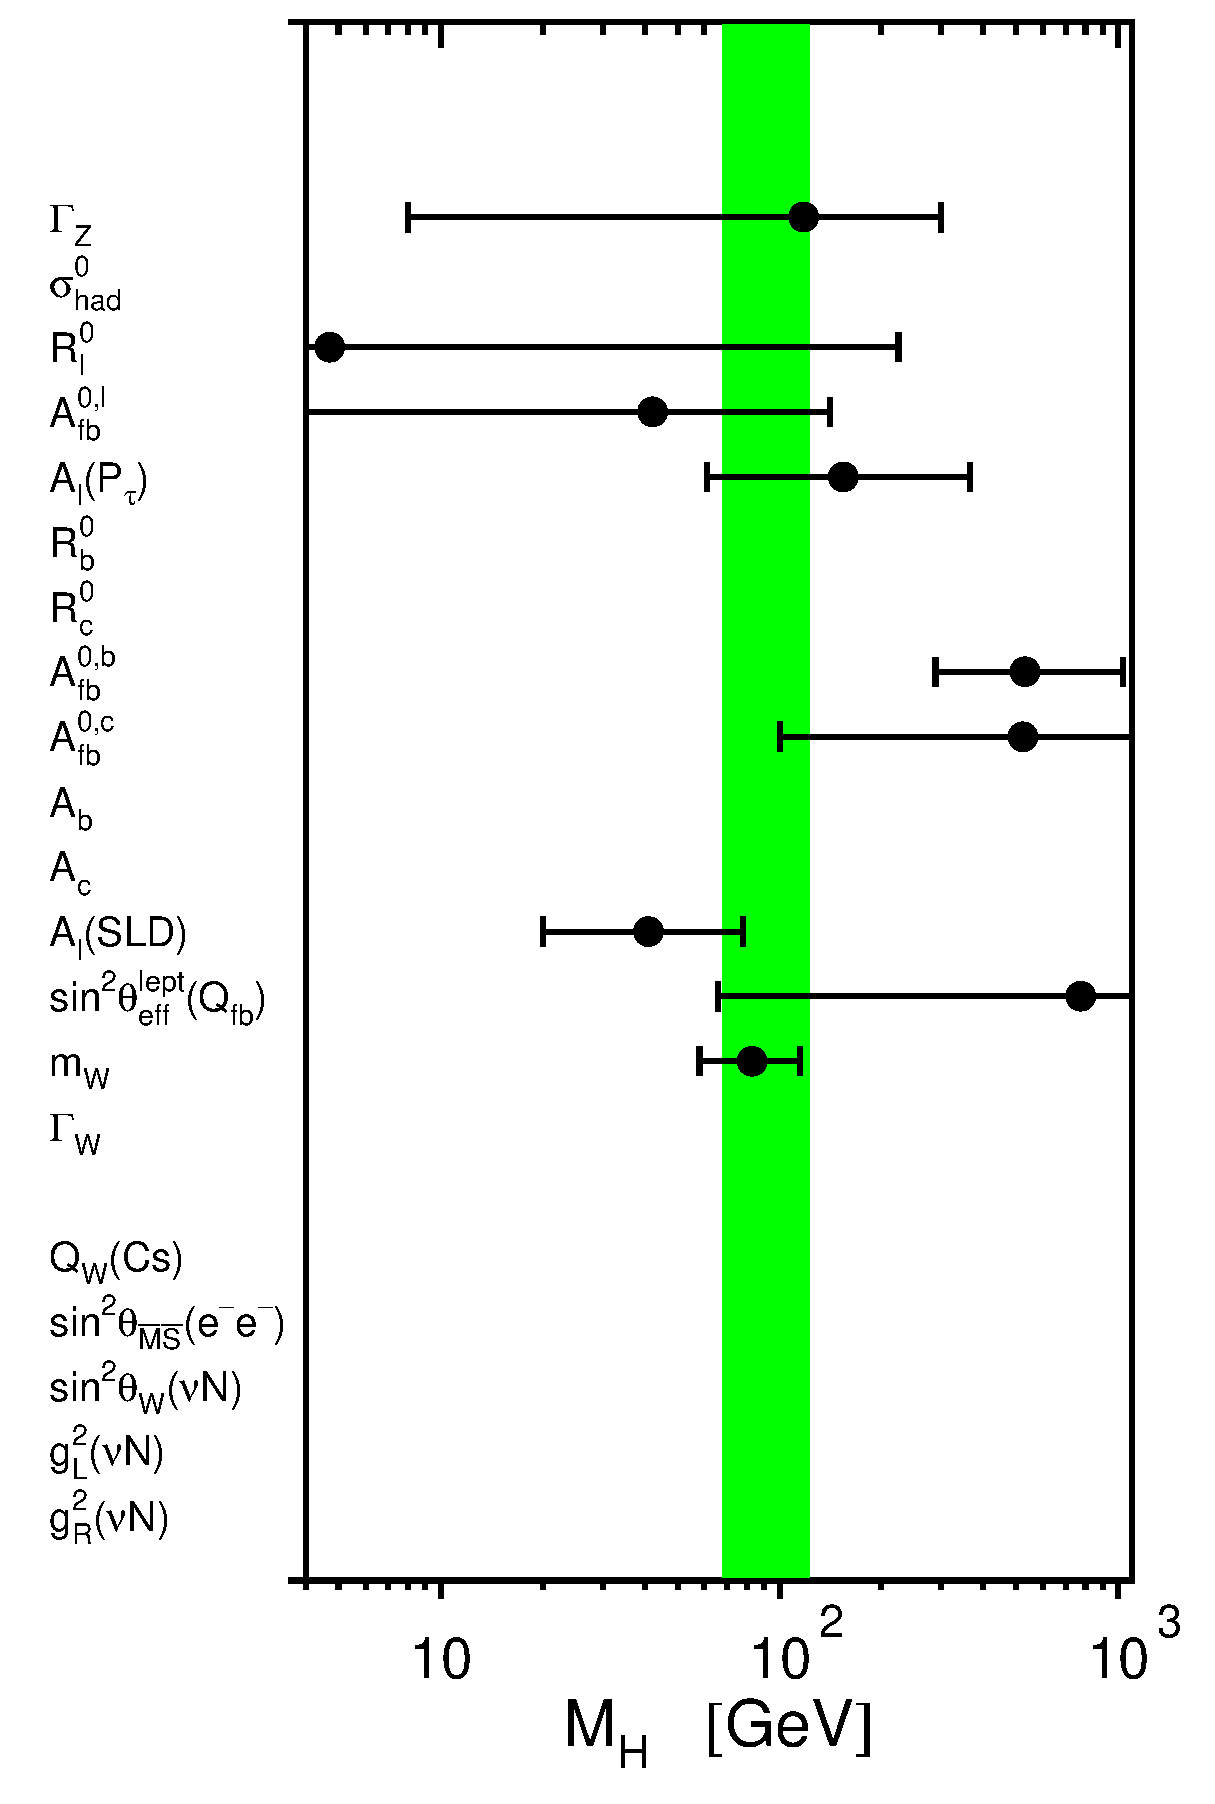
\includegraphics[height=0.4\textheight]{figures/w12_show_higgs.eps}
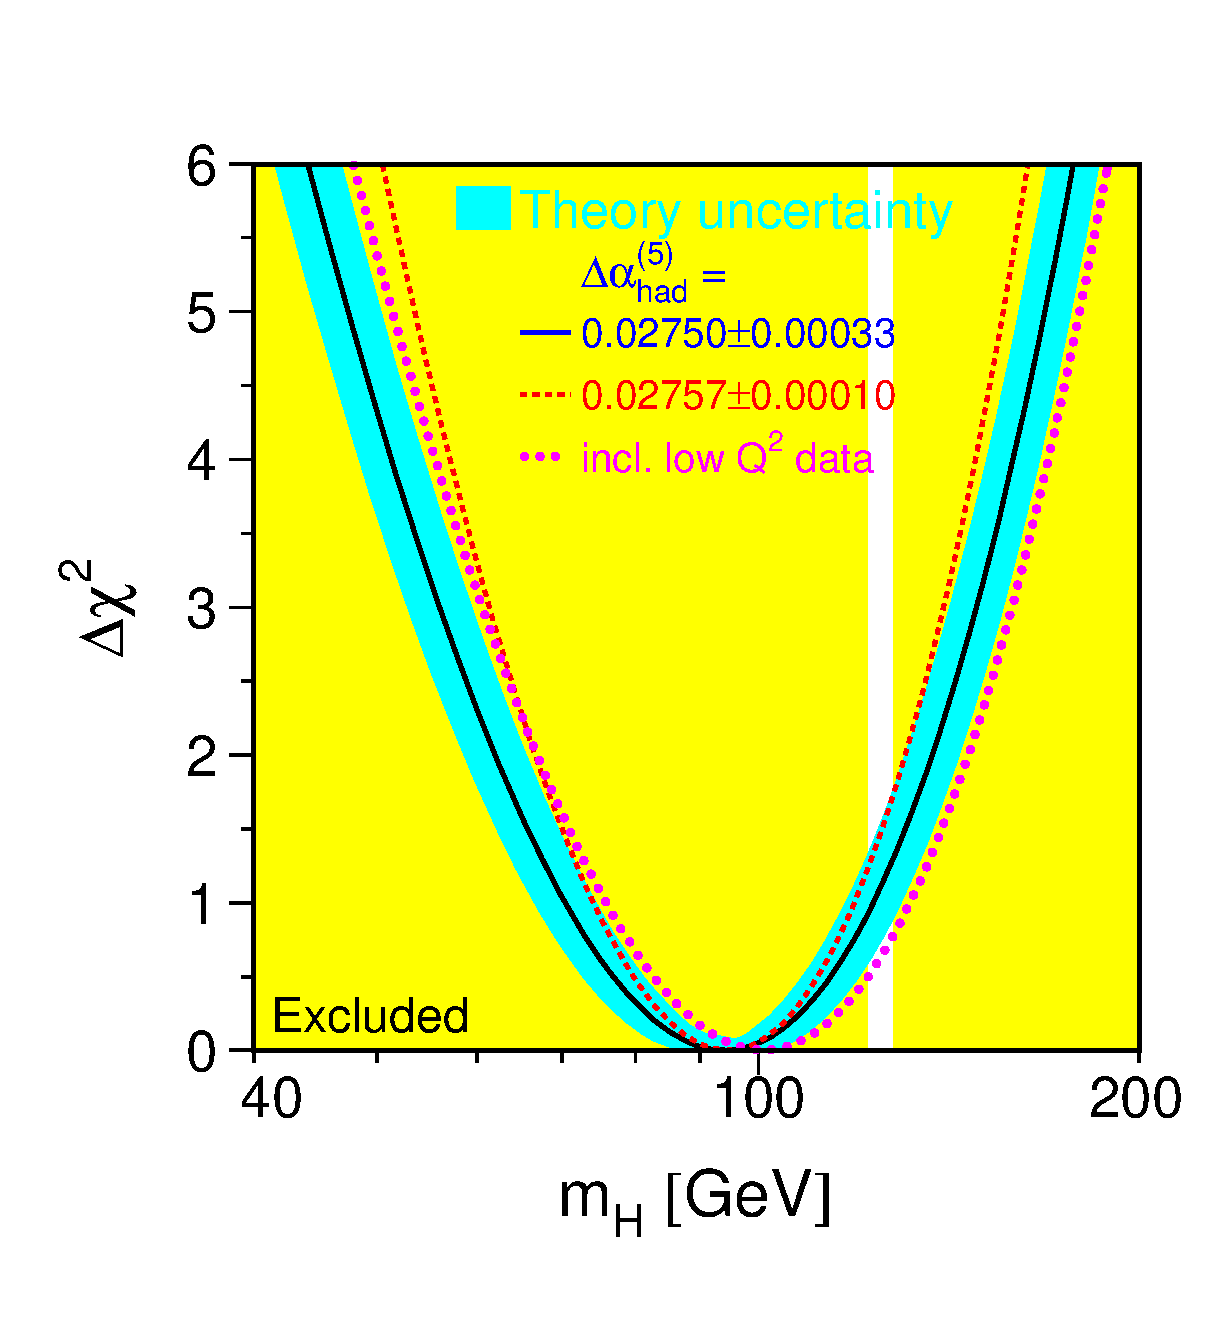
\includegraphics[height=0.5\textheight]{figures/w12_blueband.eps} % Figure F.4 in \cite{LEP-2}
\caption{$\Delta \chi^2 = \chi^2 - \chi^2_{min}$ as a function of \mHi~\cite{LEP-2}.}
\label{fig:EWKprecision}
\end{figure*}
The Figure~\ref{fig:EWKprecision} 
%top plots shows the constraints on \mHi %from each variable used by global fit, 
shows $\Delta \chi^2$ curve as a function of \mHi\ from EWK precision measurements
assuming that Standard Model is the true theory of nature \cite{LEP-2}. 
The preferred \mHi\ is $94_{-24}^{+29}~\GeV$. It also shows that 
the upper limit on \mHi\ at C.L. = 95 \% is 152 \GeV. 

%
\subsubsection{Direct search}  

Before 2012, there were direct searches for SM Higgs boson by LEP, Tevatron, 
and LHC experiments. 
The LEP data showed the limit of $\mHi>114.4~\GeV$ at \CLs = 95 \% \cite{Beringer:1900zz} 
and the Tevatron showed exclusion of SM Higgs hypothesis in the range of 
$147~\GeV < \mHi < 179~\GeV$ at \CLs = 95 \% \cite{Beringer:1900zz}. 
At the end of 2011, the LHC experiments(CMS and ATLAS) showed their results with 7~\TeV\ data
on the standard model Higgs search \cite{Chatrchyan201226,Aad201249}. 
\begin{figure}[htp]
\centering
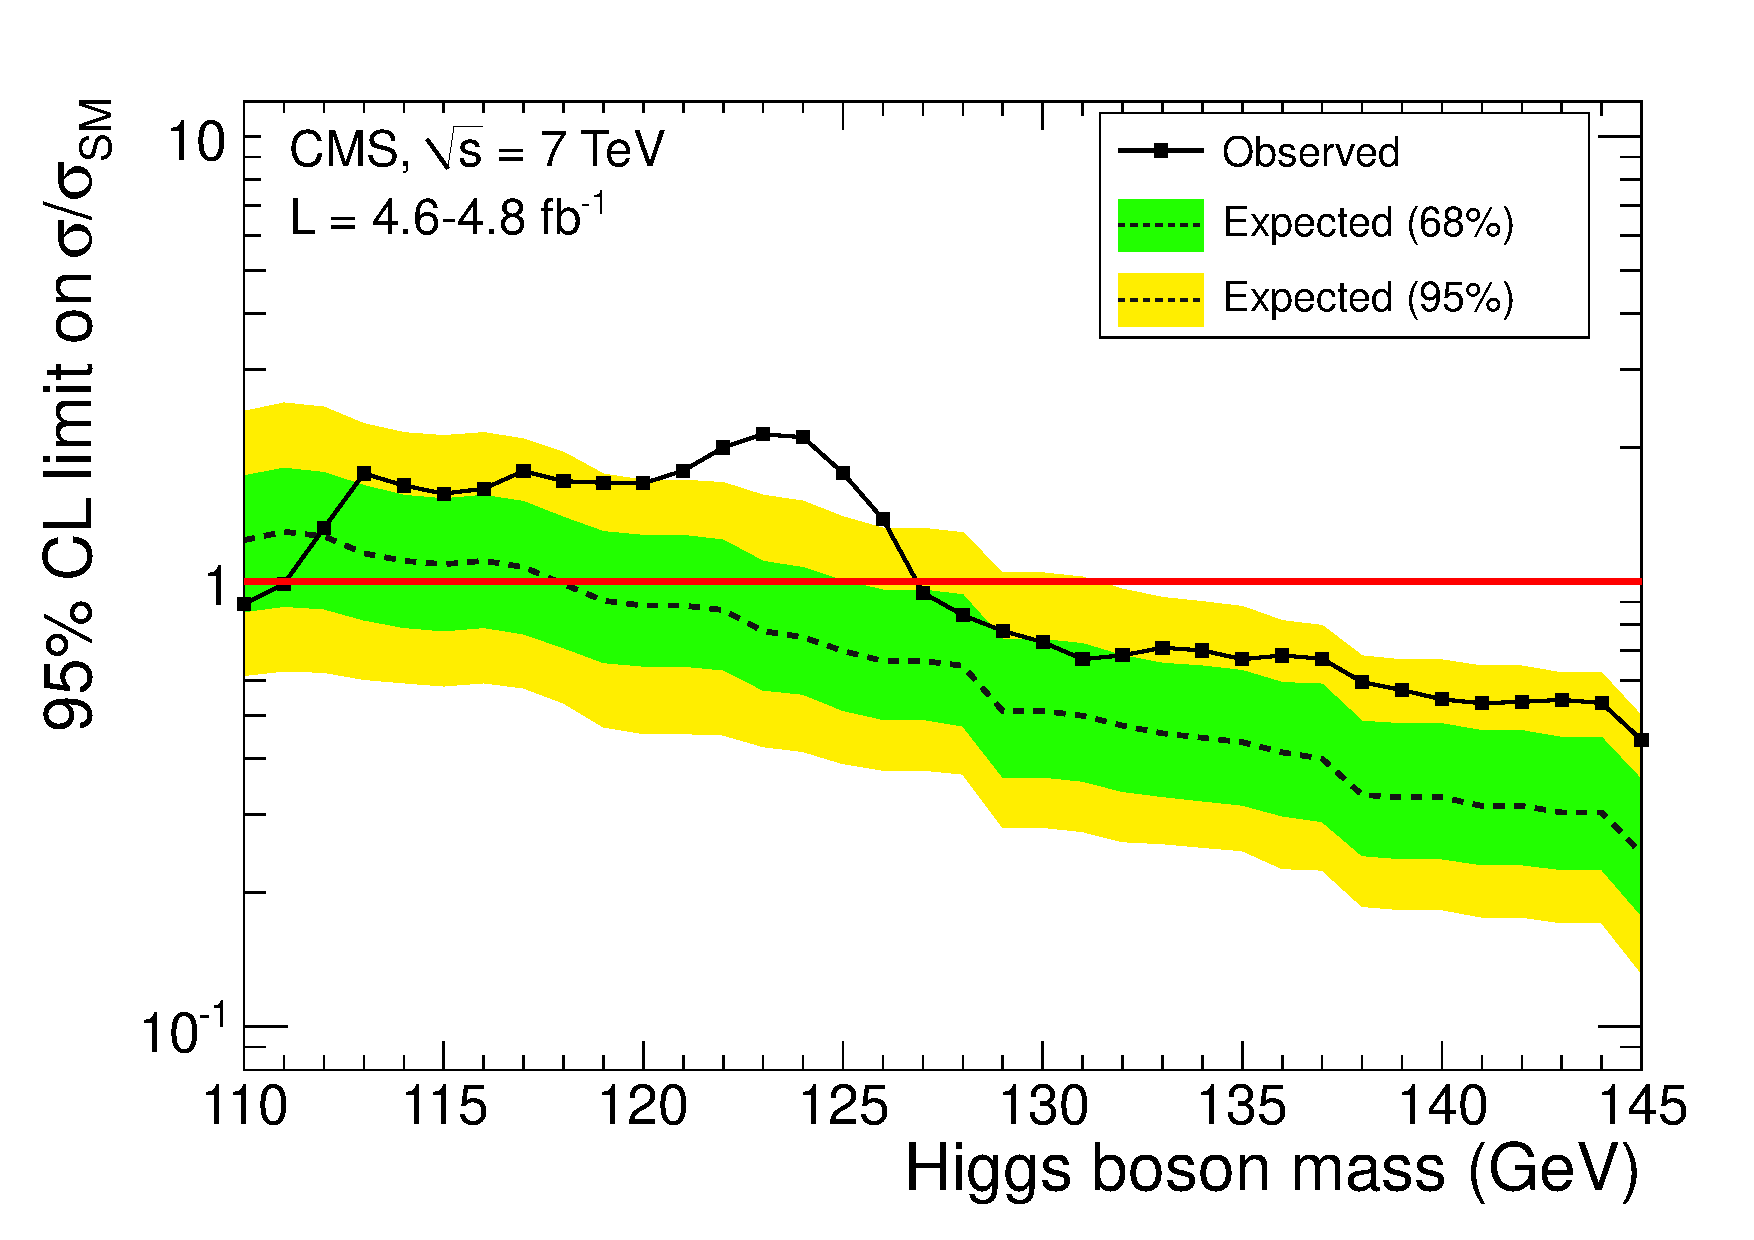
\includegraphics[width=0.45\textwidth]{figures/cls_comb_zoom.pdf}
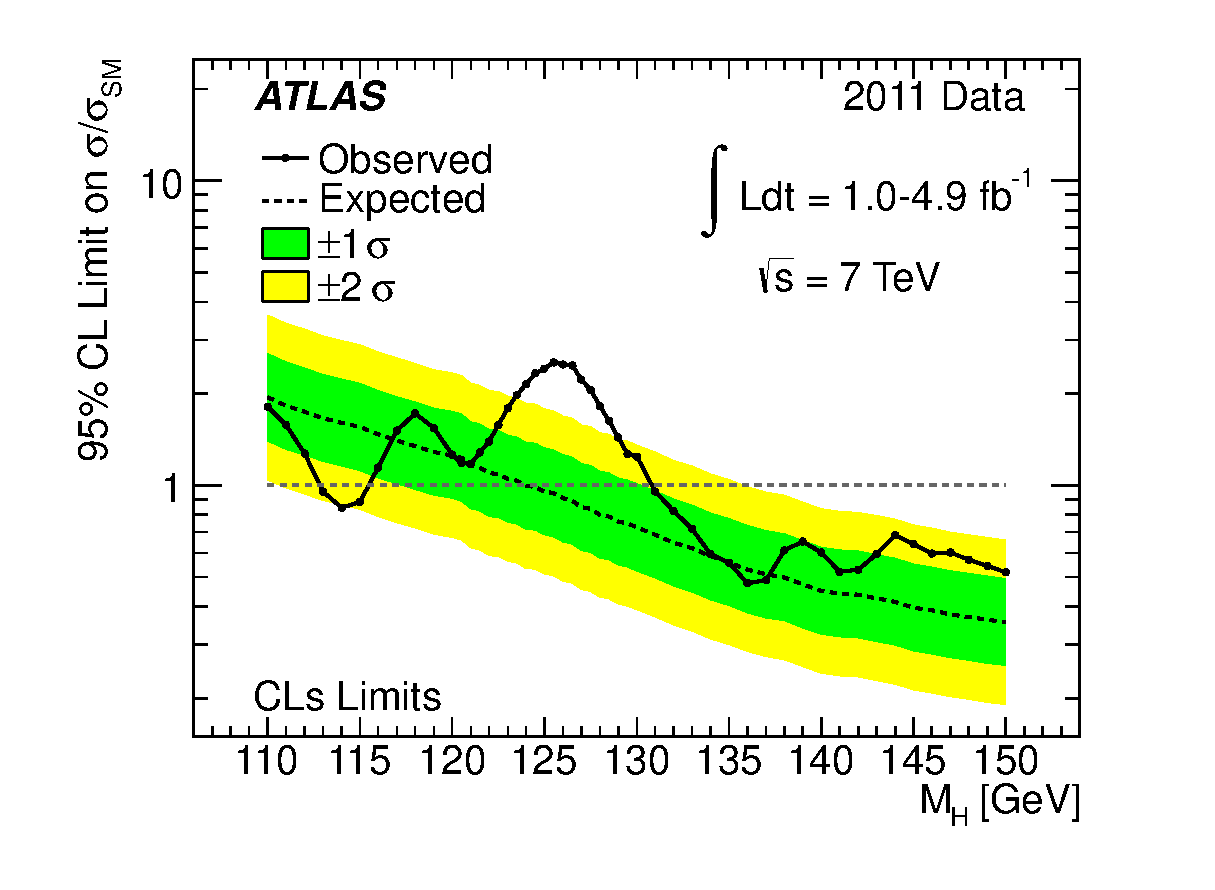
\includegraphics[width=0.45\textwidth]{figures/fig_05b.eps}
\caption{ CMS / ATLAS Higgs exclusion with 7 TeV data. }
\label{fig:2011HiggsExp}
\end{figure}
Figure~\ref{fig:2011HiggsExp} shows the 95\% C.L. upper limits on $\sigma/\sigma_{\textrm{SM}}$
as a function of \mHi\ in the range of 110 - 145 \GeV\ for CMS on the left and 
110 - 150 \GeV\ for ATLAS on the right. In both experiments, search was performed up to 
\mHi = 600 \GeV, but only low \mHi\ region is shown on the plots. 
In CMS, the observed exclusion range is 127 - 600~\GeV\ 
while the expected exclusion range is 118 - 543~\GeV.     
In ATLAS, the observed exclusion range is 131-238 and 251-466 \GeV\ 
while the expected exclusion range 124 - 519 \GeV.  
Both experiments, CMS and ATLAS, showed local excess of 
$3.1\sigma$ and $3.5\sigma$, respectively, around \mHi = 125 \GeV. 

 

%%%%
\newpage
\section{The \hww\ channel} 

The \hww\ is an important channel because of its large production rate, 
which allows a good statistical power to measure the production rate. 
It has a special event topology due to Higgs' spin being zero and 
the V-A nature of leptonic W decays. This special topology results 
in difference between signal and backgrounds in some kinematic variables
and those variables are used to separate signal from backgrounds. 
CMS performed a search for SM Higgs boson with 7~\TeV\ data
in \hww\ channel and no excess was found~\cite{Chatrchyan:2012ty}. 

%
\subsection{Large production rate}

The \hww\ channel has a good statistical power to measure $\sigma \times BR$
assuming the backgrounds can be controlled.
Figure~\ref{fig:XSBR_8TeV_SM_LM} shows $\sigma \times BR$ at $\mHi<250~\GeV$.
\begin{figure*}[t]
\centering
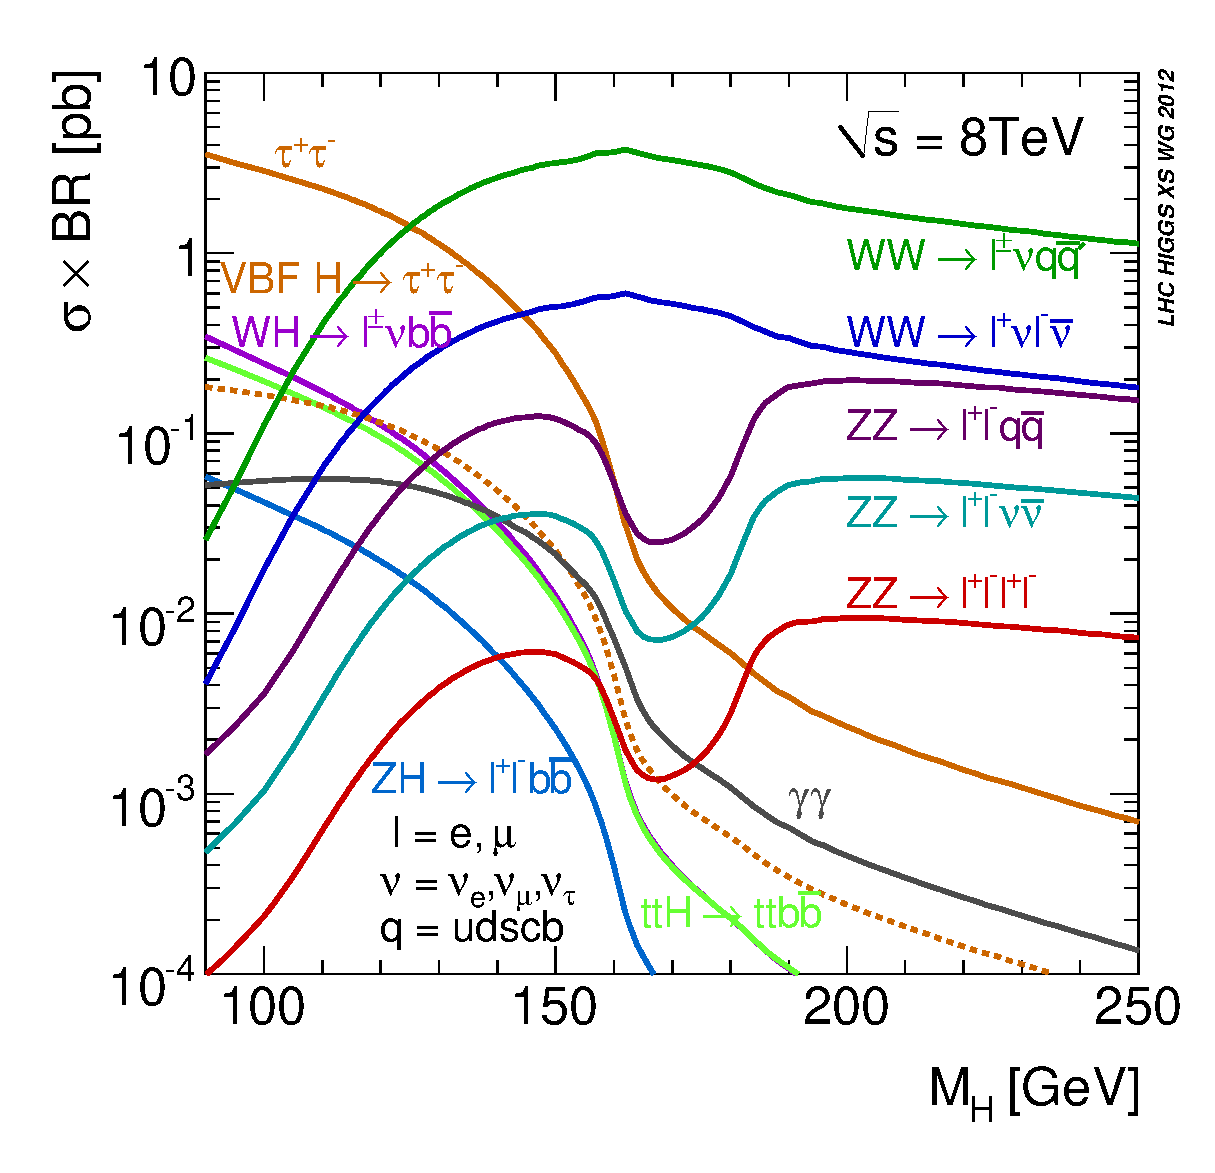
\includegraphics[width=0.6\textwidth]{figures/XSBR_8TeV_SM_LM.eps}
\caption{$\sigma \times BR$ at low \mHi.}
\label{fig:XSBR_8TeV_SM_LM}
\end{figure*}
It shows that the $\sigma \times \textrm{BR}$ of \hww\ channel 
is large compared to the other sensitive channels, $H \rightarrow ZZ\rightarrow 4l$
and $H \rightarrow\gamma\gamma$. 
\begin{table}[htb]
\centering
\label{tab:XSBR_8TeV_SM_125}
\vspace{0.5cm} 
\caption{$\sigma \times BR$ at $\mHi=125~\GeV$ for most sensitive channels 
and the expected number of events in $\mathcal{L}_{int} = 20~\ifb$.
$l$ means electrons or muons.}
\vspace{0.5cm} 
\begin{tabular}{c | c c c}
\hline 
        & $H \rightarrow WW \rightarrow 2l2\nu$   & $H \rightarrow ZZ\rightarrow 4l$ 
        & $H \rightarrow\gamma\gamma$  \\
\hline \hline 
$\sigma \times BR (pb)$  
        & $2.24\times10^{-1}$ &  $2.79\times10^{-3}$ & $5.09\times10^{-2}$ \\ 
$N_{expected}$ in $\mathcal{L}_{int} = 20~\ifb$ 
        & 4480 &  56 & 1018 \\ 
\hline 
\end{tabular}
\end{table}
Table~\ref{tab:XSBR_8TeV_SM_125} shows $\sigma \times \textrm{BR}$ for 
the most sensitive channels, \hww, $H \rightarrow ZZ\rightarrow 4l$
and $H \rightarrow\gamma\gamma$, and the expected signal events at
the integrated luminosity, $\mathcal{L}=20~\ifb$. The expected signal 
events are 4480, 56 and 1018 for \hww, $H \rightarrow ZZ\rightarrow 4l$
and $H \rightarrow\gamma\gamma$, respectively. This allows to have a 
good statistical power to measure the $\sigma \times \textrm{BR}$
with this channel. 

%
\subsection{Angular distribution of leptons in the final state}
\label{subsec:angular_dist}

The spin of SM Higgs is zero, so by helicity conservation the total spin 
of the WW system should be zero as well. 
\begin{figure}[htp]
\centering
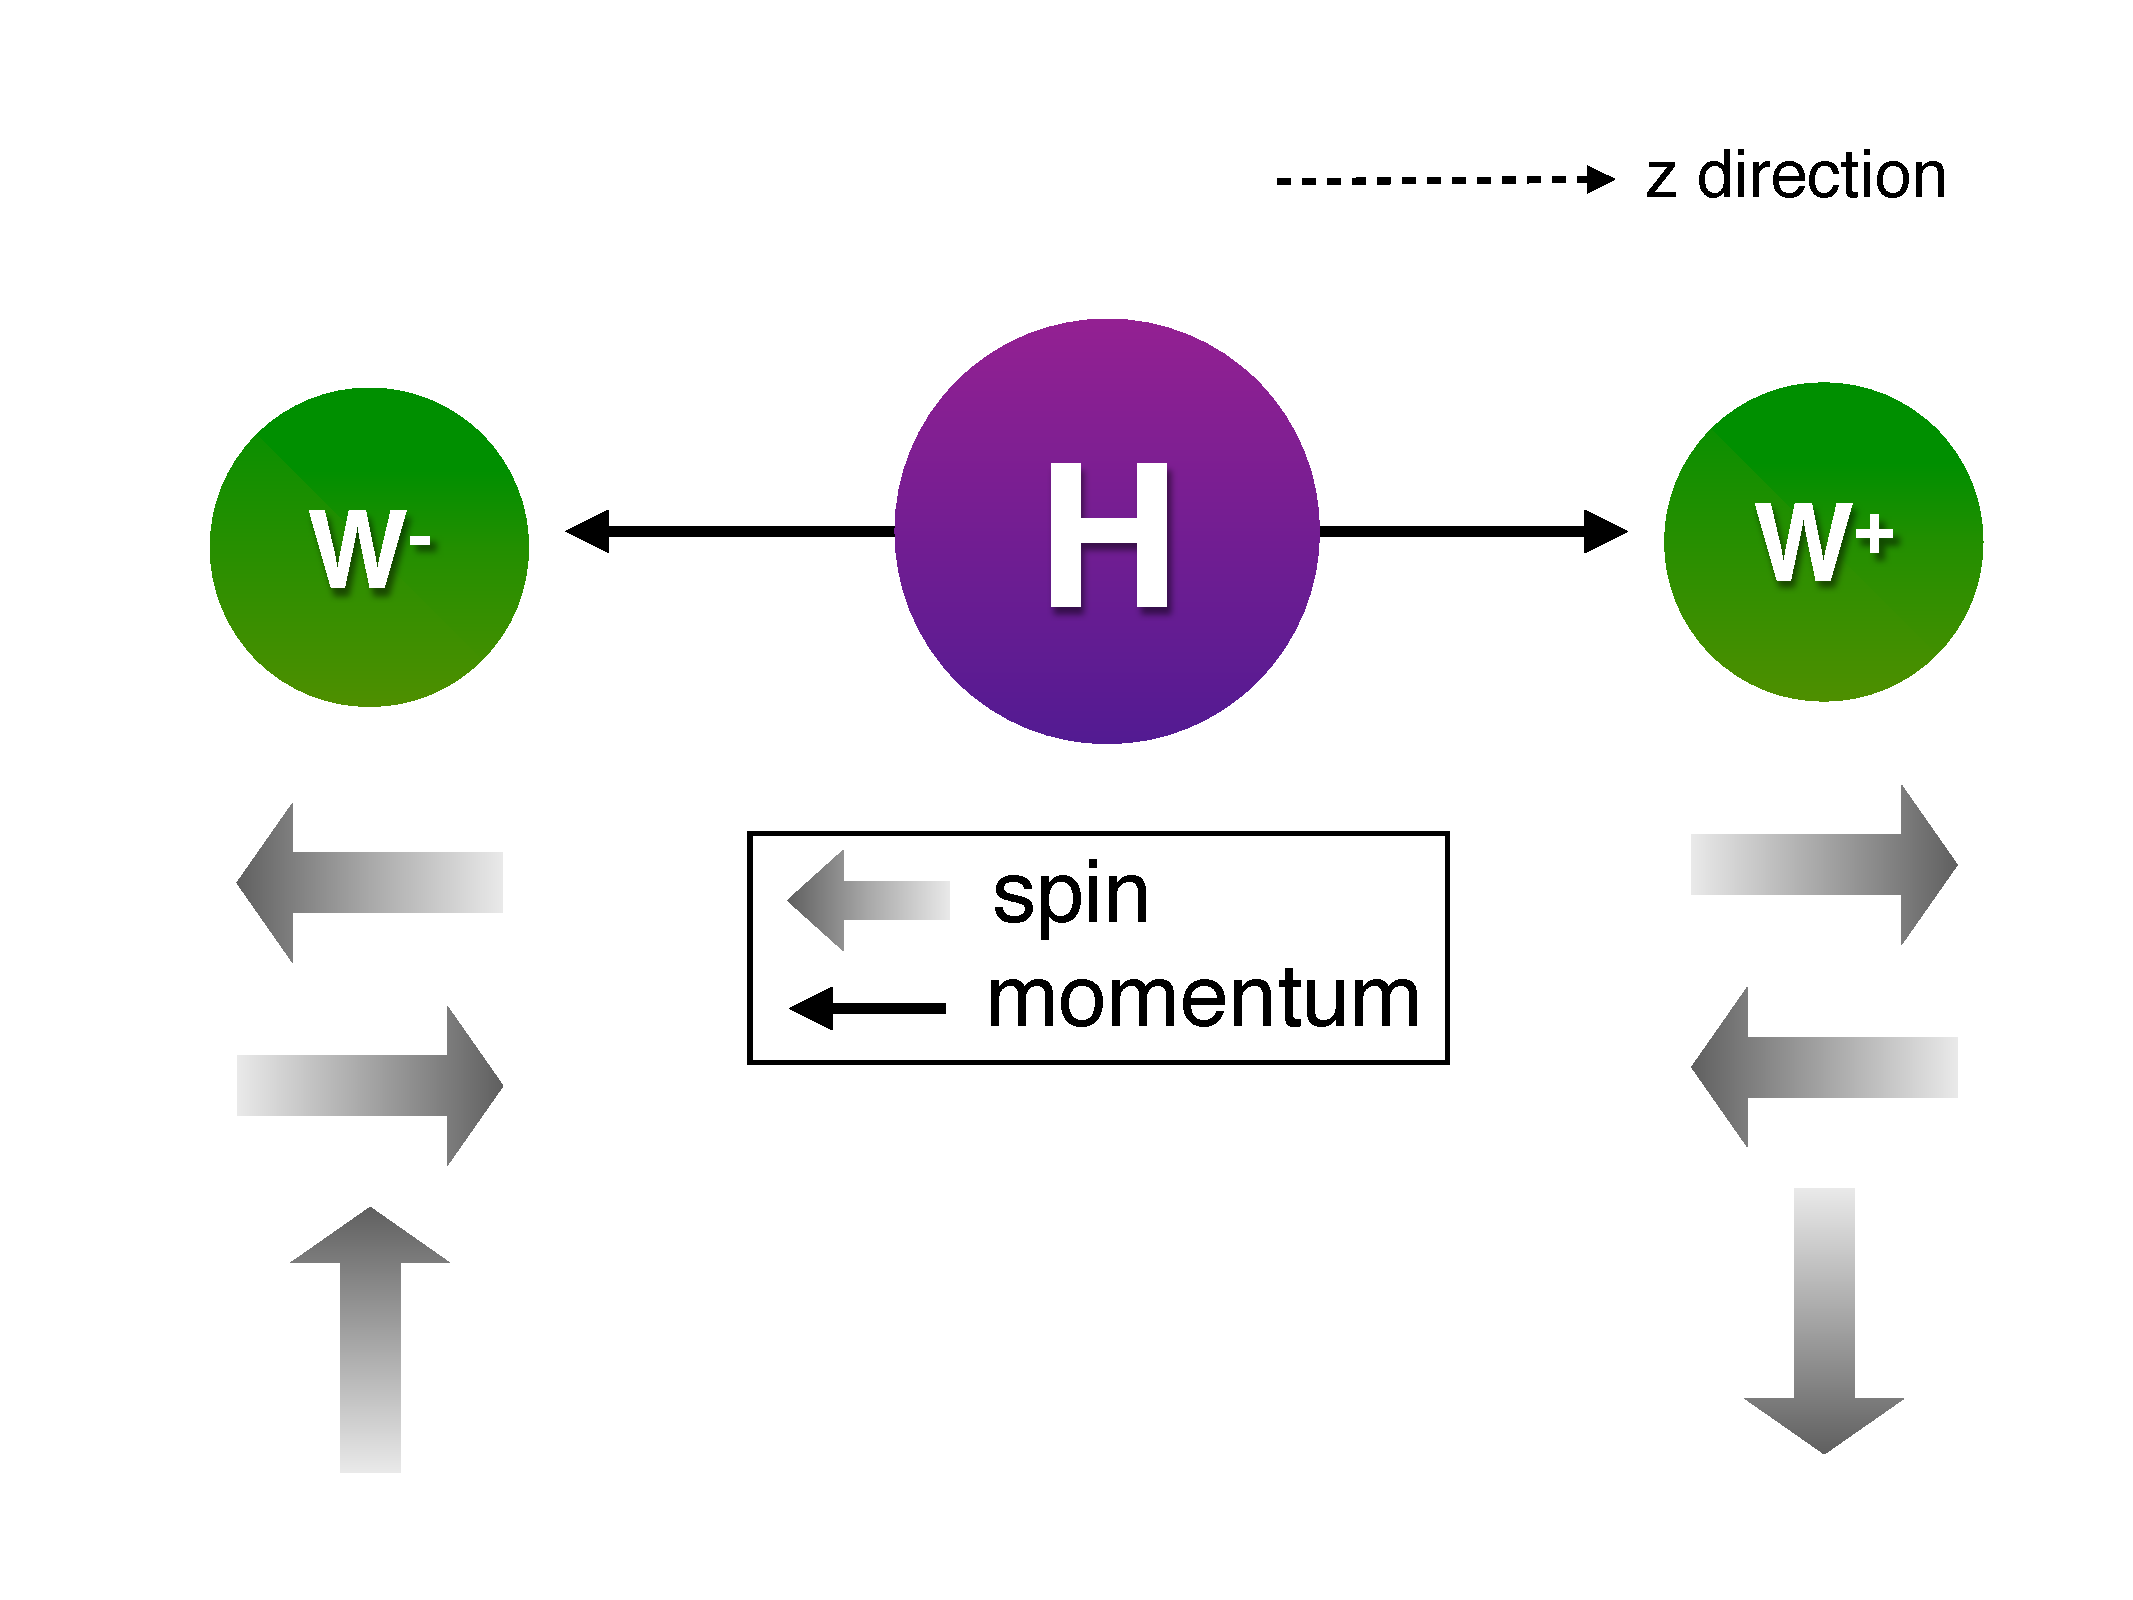
\includegraphics[width=0.7\textwidth]{figures/HiggsSpin.pdf}
\caption{Spin configuration of Higgs boson decaying to $W^+W^-$ in the CM frame of Higgs.
Solid black arrows represent momentum direction of Ws and grey arrows indicate 
the spin configuration.}
\label{fig:HiggsSpin}
\end{figure}
As shown in Figure~\ref{fig:HiggsSpin}, if we take 
the direction of $W^+$ momentum as z axis in the center-of-mass(CM) frame of Higgs boson,
there are two cases where the spin direction is parallel to the 
momentum direction (transverse polarization) and one case where 
it is perpendicular to the momentum direction(longitudinal polarization). 
In case of transverse polarization, the leptons from Ws have strong 
angular dependence due to V-A nature of weak decays, i.e. neutrinos 
are always left-handed(anti-neutrinos are always right-handed). 
Let's take the case of $W^+$ spin in the z direction as an example.
In order for the neutrino from $W^+$ to be left-handed, the direction 
of the neutrino should be in the - z direction, thus lepton should 
fly to z direction. In order for the anti-neutrino from $W^-$ to be 
right-handed, the direction of the anti-neutrino should be in the 
- z direction, thus lepton should fly to z direction.
Therefore, both leptons tend to move in the same direction 
resulting in a small angle between the two leptons. 
This is somewhat diluted due to boost of Higgs and Ws, 
but the effect is still visible and used to separate signals 
from non-resonant WW background. 
On the other hand, in case of longitudinal polarization, 
no specific angular correlation is present. 
As discussed in section~\ref{sec:decayHiggs}, the fraction of longitudinal 
polarization depends on the Higgs mass. So, we expect that the two leptons 
in the final state tend to be more aligned at \mHi\ where the fraction of longitudinal 
polarization is small. 


%
\subsection{Kinematic variables}
\label{subsec:kinimetic_variables}

\begin{figure}[htp]
\centering
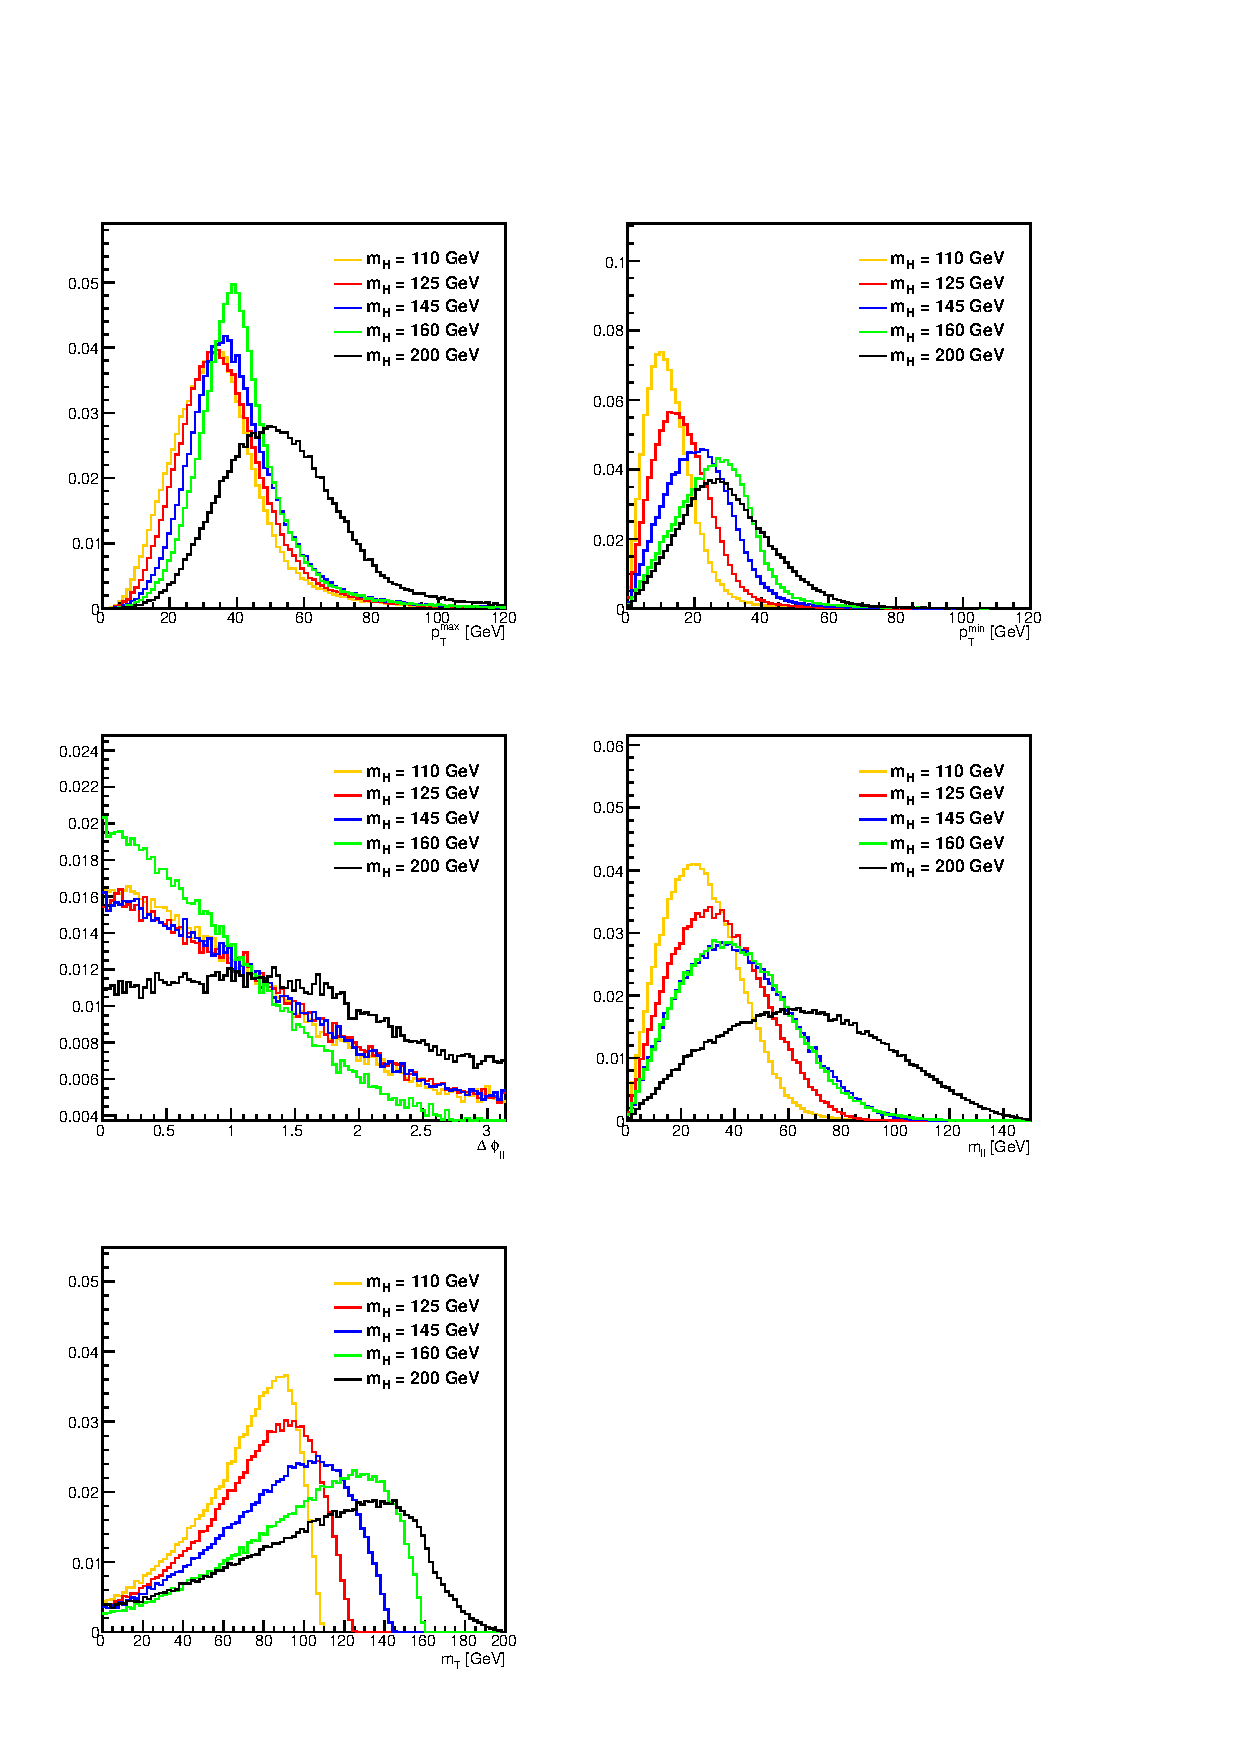
\includegraphics[width=0.9\textwidth]{figures/hww_gen_all.pdf}
\caption{Kinematic distributions of \ptlmax, \ptlmin, \delphill, \mll\ and \mT, 
for $\mHi = 110, 125, 145, 160\textrm{ and } 200~\GeV$ at the generator level.}
\label{fig:genhww}
\end{figure}
Figure~\ref{fig:genhww} shows distributions of kinematic variables for 
multiple Higgs hypotheses, $\mHi = 110, 125, 145, 160\textrm{ and } 200~\GeV$. 
The plotted variables are leading and trailing lepton \pt (\ptlmax, \ptlmin), 
azimuthal angle difference between the two leptons (\delphill), 
di-lepton invariant mass (\mll), and Higgs transverse mass (\mT) which is 
defined as 
\begin{eqnarray} 
\mT = \sqrt{2\ptll\met(1-cos(\Delta\phi_{\ell\ell-\met}))}
\end{eqnarray} 
where \ptll\ is transverse momentum of the di-lepton system, 
\met\ is missing transverse momentum, and  
$\Delta\phi_{\ell\ell-\met}$ is the angle between the momentum of di-lepton
system and \met\ in the transverse plane.
Most of the events have \ptlmax\ greater than 20~\GeV\ for all \mHi\ hypotheses. 
\ptlmin\ is quite populated at low \ptlmin\ region, especially for low \mHi\ 
hypotheses. In case of \mHi = 125~\GeV, approximately 25 \% of 
events are rejected by requiring $\ptlmin>10~\GeV$. 
\delphill\ shows non-straightforward trend. The angle tends to get smaller 
as \mHi\ increases up to 160 \GeV, and the angle becomes wide 
after \mHi = 160~\GeV. This behavior was expected in the 
Figure~\ref{fig:HVV_polarization_ratio} where the fraction of the 
longitudinal polarization is at the minimum at \mHi = 2\mW\ which is about 160~\GeV. 
Since small \delphill\ yields small \mll\, we expect small \mll\ 
for low \mHi\ hypotheses. The Higgs transverse mass \mT\ shows clear 
drop at \mHi. 
%\textcolor{red}{why tail and lazy drop at 200 GeV?}, 

%
\subsection{CMS \hww\ result before 2012}

Before 2012, 4.6 \ifb\ of data at $\sqrt{s}=7~\TeV$ collected by CMS detector 
was analyzed for SM Higgs search in \hww\ channel~\cite{Chatrchyan:2012ty}. 
\begin{figure}
\centering
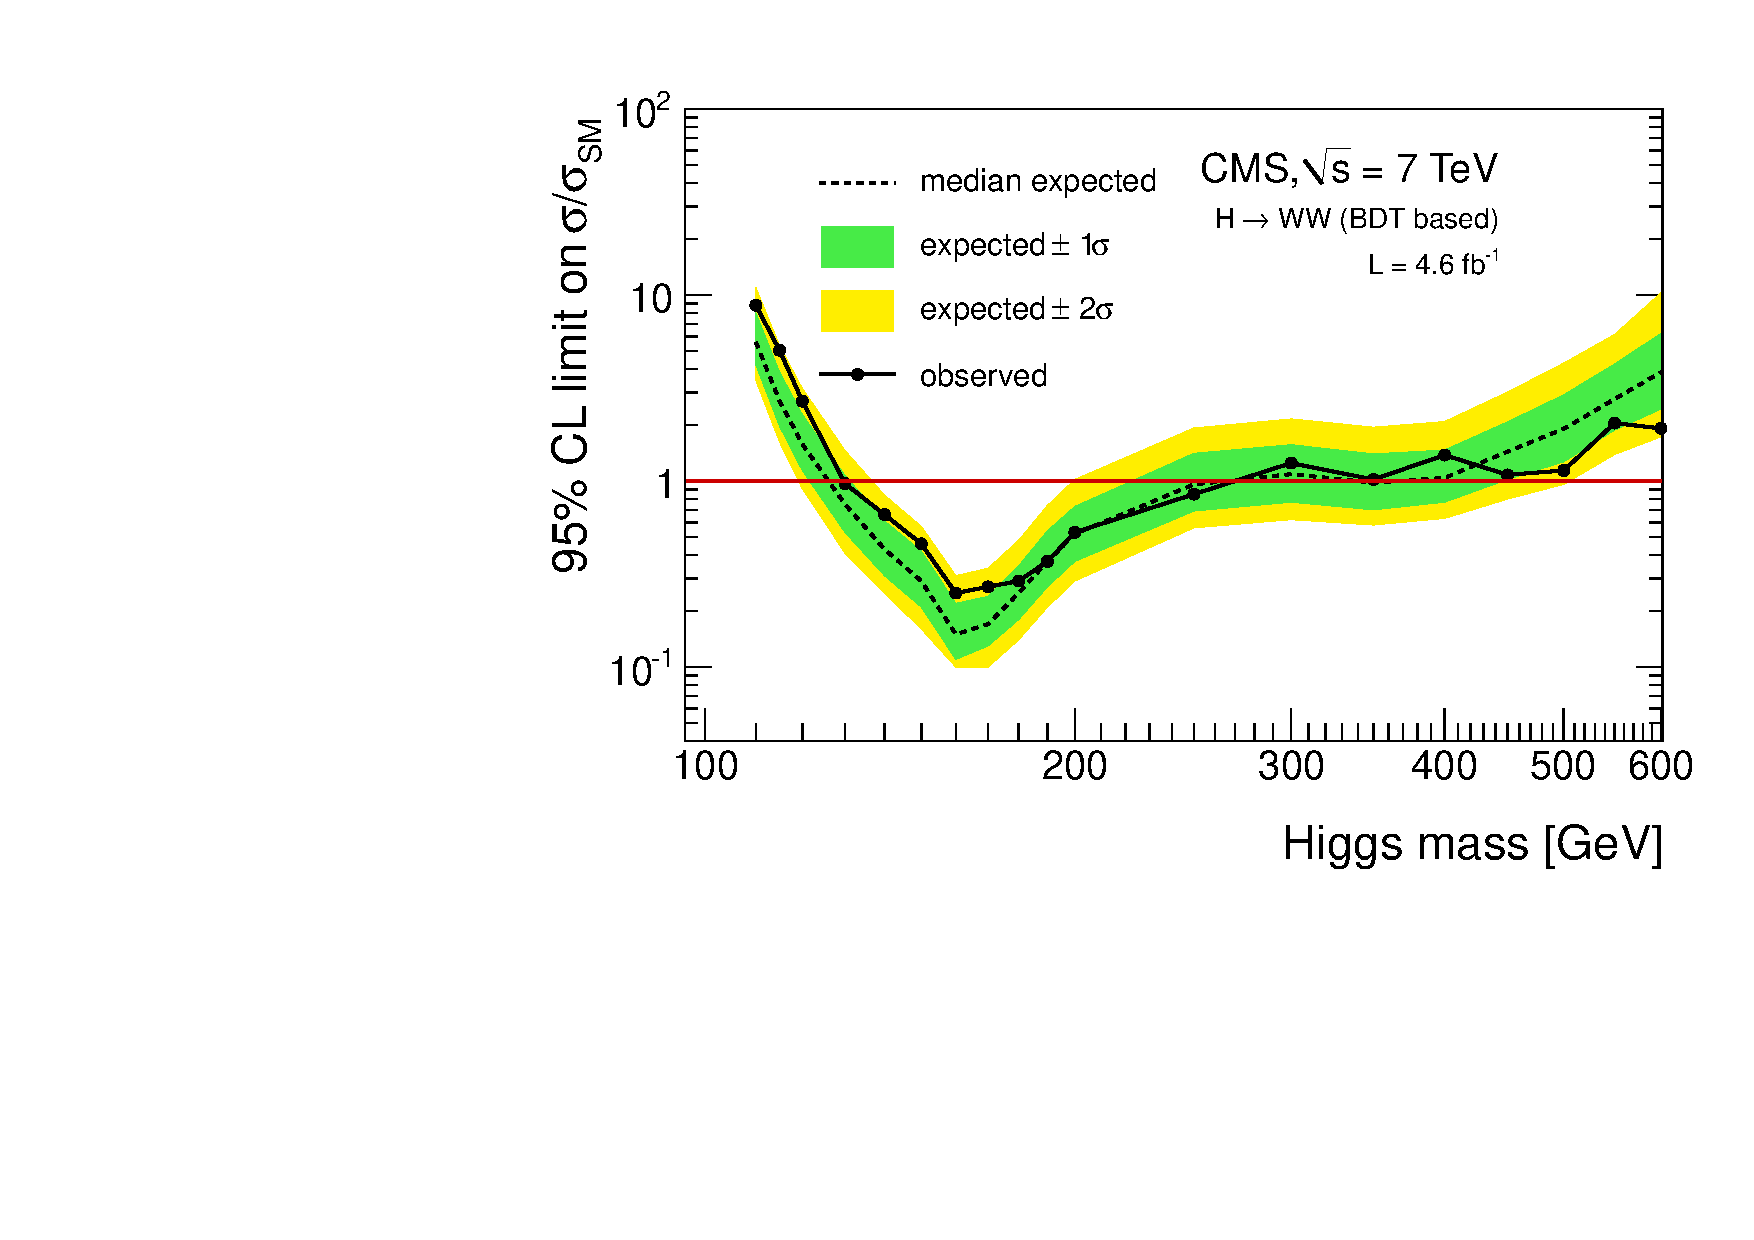
\includegraphics[width=0.9\textwidth]{figures/limits_nj_shape.pdf}
\caption{ Exclusion limit of SM Higgs with 2011 data($\sqrt{s}=7~\TeV$, $\mathcal{L}=4.6~\ifb$ ).
The observed(expected) exclusion limit at CL  = 95 \% is \mHi = 129 - 270(127 - 270) \GeV.}
\label{fig:hww2011}
\end{figure}
Figure~\ref{fig:hww2011} shows exclusion limit of SM Higgs boson 
using a multivariate technique based on the boosted decision tree(BDT) algorithm~\cite{Chatrchyan:2012ty}.
The observed exclusion limit at \CLs  = 95 \% is \mHi\ = 129 - 270 \GeV\
with expected limit \mHi\ = 127 - 270 \GeV. There is a slight overall excess 
in low \mHi\ region which might indicate existence of SM Higgs boson at low \mHi.  



%
\chapter{LHC and CMS Detector}
\label{ch:lhc_cms}
\section{Large Hadron Collider} 

Overview of accelerator
* How protons are generated 
* Steps to get accelerated 
* Luminosity determination 

\section{Compact Muon Solenoid detector} 
\subsection{Tracker : pixel and silicon detector}
\subsection{ECAL} 
\subsection{HCAL} 
\subsection{Magnet} 
\subsection{Muon System} 
\subsection{Forward : HF}                
\subsection{Computing : grid computing} 



%
\chapter{Event Reconstruction}
\label{ch:event_reconstruction}

The information such as hits in the tracker and the muon system,
and the energy deposit in the calorimeters which is collected by 
sub-detectors is used to reconstruct objects. Using the available 
information, we can reconstruct stable particles such as 
electron, muon, pion, kaon and photon, and other objects 
used to select and distinguish signal events from backgrounds. 
This chapter discusses how these objects are reconstructed. 
\textcolor{red}{work on introduction a little bit more} 

%%%%%%%%%%%%%%%%%%%%%%%%%%%%%%%%%%%%%%%%%%%%%%%%%%%%%%%%%%%%%%%%%%
\section{ Tracks }
\label{sec:track}
%\textcolor{red}{This is for barrel only. 
%Ref : note005\_001.pdf chapter 2. need to check the endcap case.}

When a charged particle($e^\pm, \mu^\pm, \pi^\pm, ... $) traverses in the tracker,
it leaves hits in the pixel and the silicon layers. By collecting those hits
that are consistent with each other, we can reconstruct the 
trajectory of the particle, and eventually calculate its momemtum. 
The reality is not that simple though, because there are multiple 
particles in an event, and a random combination can fake a particle track.  
Interactions with the material in the tracker can change the 
direction and the magnitude of the momentum of particles. 
In addition, there are uncertainties to the sensors that 
can result in no hits in a silicon layer even though a charge 
particle passed it. Therefore, we should consider these points 
when reconstructing tracks from the hits in the tracker. 

The CMS uses the Combinatorial Track Finder(CTF)~\cite{} as a general tracking 
algorithm, and this section describes the procedure in detail.


\subsubsection{Generation of seeds : finding starting points}

The reconstruction of a track starts with seeding, \textit{i.e.} 
finding the initial values of the track parameters. 
The seeds can be obtained from the tracking system itself or from external systems.  
The CMS takes an approach to obtain the seed from the innermost layer 
of the tracker, and find track candidates starting from inside to outside. 
The most important reason for this choice is that the 
charged particles have interactions as they fly out,
and a non-negligible amount of materials in the tracking system 
that the particle should go through changes their initial momentum.
Therefore, in order to reduce the effect of materials as much as possible, 
we start from the innermost layer for track finding. 
This means that the seed needs to be obtained before the innermost 
layer of the tracker. Most of the charged particles cross the 3 layers 
\footnote{At least 3 hits or 2 hits plus a beam spot are needed to 
fully determine the five track parameters.}
%(\textcolor{red}{trajectory curvarture,
%impact parameter, polar angle, azimuthal angle at the closest approach, 
%and z position at the closest approach}).
of pixel detector, so the seeds are obtained from the triplets of the 
pixel measurements. 
However, because of the geometry of the pixel detector 
and the inefficiency of the pixel readouts, 
the seeds are also obtained from combining information from the pixel layers, 
the vertex/beam spot and the hits in the strip layers \cite{cmstdr1}.   

\subsubsection{Pattern recognition : finding track candidates}

Using the obtained seed, the Kalman filter~\cite{Fruhwirth1996189} 
is used to find tracks. 
From the seed layer, the filter proceeds to the next layer using coarse 
track parameters obtained from the seed. Starting from the seed, this is done 
layer after layer updating the trajectory information after each layer. 
At each layer, the filter is executed in the following steps. 

First, with given the trajectory state, 
it is determined that which of the adjacent layers are expected 
to be crossed by extrapolating the trajectory. Second, the detectors 
that are compatible with the trajectory are determined. Third, 
for each compatible detector, compatible measurements are searched 
by calculating the drift of charge carriers inside the silicon 
in order to improve position measurements. $\chi^2$ test is used 
to select compatible hits. Fourth, if the measurement is compatible 
with the trajectory, the track candidate includes this measurement, 
and the track parameters are updated. When there are multiple measurements
compatible with the trajectory, the several new trajectories are 
created. In addition, to account for the case where a charged particle 
passes the layer without leaving any hits(invalid hit), 
one additional track is created without adding position measurements.  
Due to an exponential increase of the number of track candidates, 
the maximum number of track candiates at each step is limited 
using $\chi^2$, and the number of valid and invalid hits. 

This procedure is repeated to the next tracker layer until either the 
outermost tracker layer is reached or the track does not satisfy the requirements
on the number of added layers and uncertainty on the track parameters.
As the iteration proceeds, the uncertainty on the position measurements 
in the $r-\phi$ plane improves due to having larger lever arm 
as the filter goes inside-out. But, the uncertainty in the $r-z$ 
becomes larger due to the geometry of double-strip layers
(longer overlap in the z direction) and absence of z measurements 
in the single-strip layers where the length of the strip (10-20~cm) is 
used to constrain the track. 
%The uncertainty on the extrapolated 
%trajectory affects the number of compatible measurements.    

%Mention barrel-endcap transition (where exactly it is? in eta ) region issue 

When many hits are present in the tracker, 
there is a large probability that the same track is reconstructed 
multiple times (duplicate tracks) from different seeds. 
So, it is important to select only one track candidate among them 
in order to avoid reconstructing the same track multiple times. 
Two tracks are considered duplicate if the fraction of the shared hits 
($f_{shared}$) is greater than 50\%.  $f_{shared}$ is defined as 
\begin{eqnarray} 
f_{shared} = \frac{N_{shared}^{hits}}{min (N_1^{hits}, N_2^{hits}) }  
\end{eqnarray}  
where $N_{shared}$ is the number of shared hits and $N_{1(2)}^{hits}$ 
is the number of hits for track candiate 1(2). If $f_{shared}$ is 
greater than 0.5, the track candidate with larger number of hits is selected. 
In case there are same number of hits in both tracks, the track with higher $\chi^2$
is selected. This cleaning continues until none of the track pairs share more than 
50 \% of their hits.  


\subsubsection{Track fit : filtering and smoothing}

From the pattern recognition explained in the previous subsection, 
we obtained a list of hits and track parameters 
with associated covariance matrix for each trajectory. 
Because the track parameters can be biased 
by the contraints imposed at the seeding stage, the track is refitted 
using a combination of the Kalman filter and the smoother
which work inside-out and outside-in, respectively. 

The Kalman filter starts at the innermost layer with the trajectory 
parameters obtained from the seed, using the covariance matrix scaled 
by a large factor.  
At a given layer, the track parameters and the covariance matrix are updated
accounting for the energy loss and multiple scattering in the material.
The procedure continues to the last hit.

The smoother starts from the outermost hit, 
and move backward to the center of the detector. 
It uses the track parameters from the Kalman filter as the starting condition 
using the covariance matrix scaled by a large factor. 
At a given hit, the updated parameters of smoother is combined (as a weighted mean) 
with the predicted parameters of the Kalman filter(excluding the current hit, 
the extrapolation starts from the innermost hit).
%\textcolor{red}{what is the defition of weight?} 

\subsubsection{Track selection : rejecting bad guys }

In the average LHC events with jets, the track finder procedure yields 
a significant fraction of fake tracks, \textit{i.e.}, a random combination 
of hits that results in a track. These are rejected by applying 
quality cuts on track \Eta, \pt, $\chi^2$ per n.d.f., impact parameters,
significance of impact parameters
and the number of crossed layers \cite{cmsnotetrackfilter}. 

\subsubsection{Iterative tracking}

In order to attain a high tracking efficiency and a low fake rate, 
the CMS developed an iterative tracking procedure \cite{cmsnoteiterativetracking}. 
The basic idea is to select the high quality tracks first and 
to find tracks that do not make the high quality tracks 
but still are good tracks that should be reconstructed. 
There are 6 iterations in CMS, and the main difference is 
the initial seeding. For example, the zeroth interation uses 
the triplet of pixel detector, and the first iteratioin uses 
pixel-pair seeding to recover tracks that failed to make 
the pixel triplet requirment. In addtion, the track parameters 
are different to maximize the performance.


\begin{figure}[htp] 
\centering 
\begin{tabular}{c} 
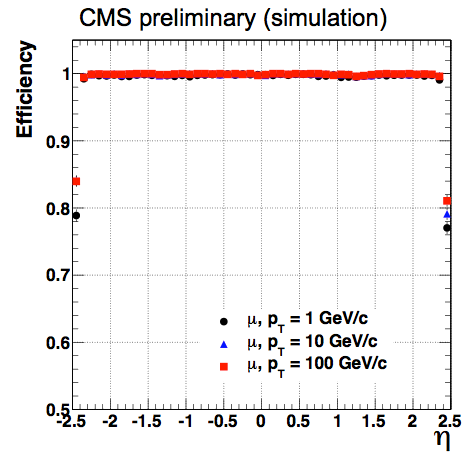
\includegraphics[width=0.45\textwidth]{figures/eff_muon_vs_eta.png} 
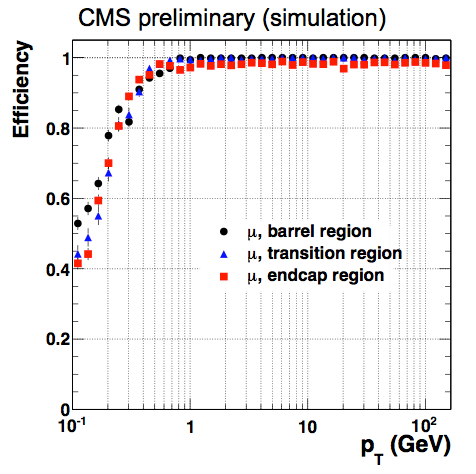
\includegraphics[width=0.45\textwidth]{figures/eff_muon_vs_pt.png} \\
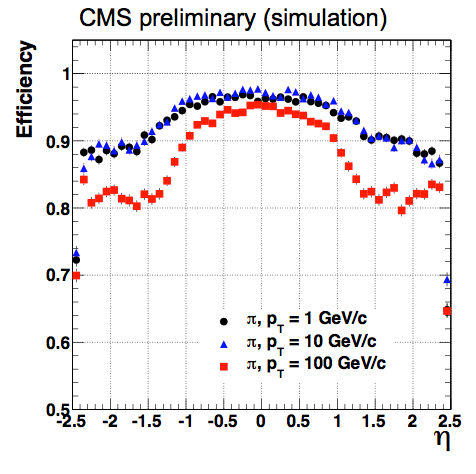
\includegraphics[width=0.45\textwidth]{figures/eff_pion_vs_eta.png} 
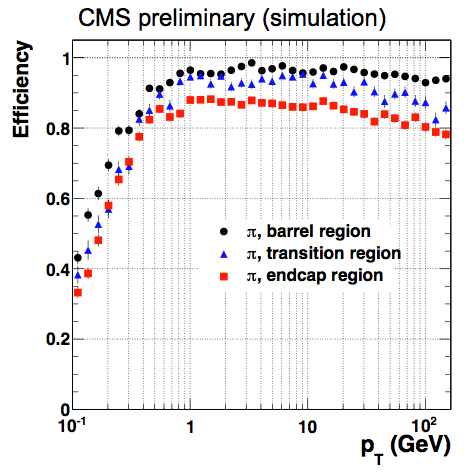
\includegraphics[width=0.45\textwidth]{figures/eff_pion_vs_pt.png} 
\end{tabular}
%https://twiki.cern.ch/twiki/bin/view/CMSPublic/PhysicsResultsTRK
\caption{Tracking efficiency measured using single pion 
and single muon simulation~\cite{TrkPerform}. 
Top left plot shows the efficiency of muon track reconstruction as a function of \Eta\
for muon \pt\ = 1, 10 and 100~\GeV. 
Top right plot shows the efficiency of muon track reconstruction as a function of \pt\
for different \Eta\ regions. 
Bottom left plot shows the efficiency of pion track reconstruction as a function of \Eta\
for pion \pt\ = 1, 10 and 100~\GeV. 
Bottom right plot shows the efficiency of pion track reconstruction as a function of \pt\
for different \Eta\ regions. 
These plots show that the tracking efficiency for muons is very close to 100~\% 
in the region of phase space we are interested in for this analysis
($\pt>10~\GeV$ and $|\Eta|<2.4$). Efficiency for pion is lower than the one for muon 
because pions decay in flight($\pi^+\to\mu^+\nu_\mu$).  
% pi+ -> mu+ nu_mu (~ 100%, ctau = 7.8 m) 
% simple calculation : e^{-1/7.8} = 0.88 
% about 12% of pions decay in the tracker
} 
\label{fig:TrackingEffMC} 
\end{figure} 

\begin{figure}[htp] 
\centering 
\begin{tabular}{c} 
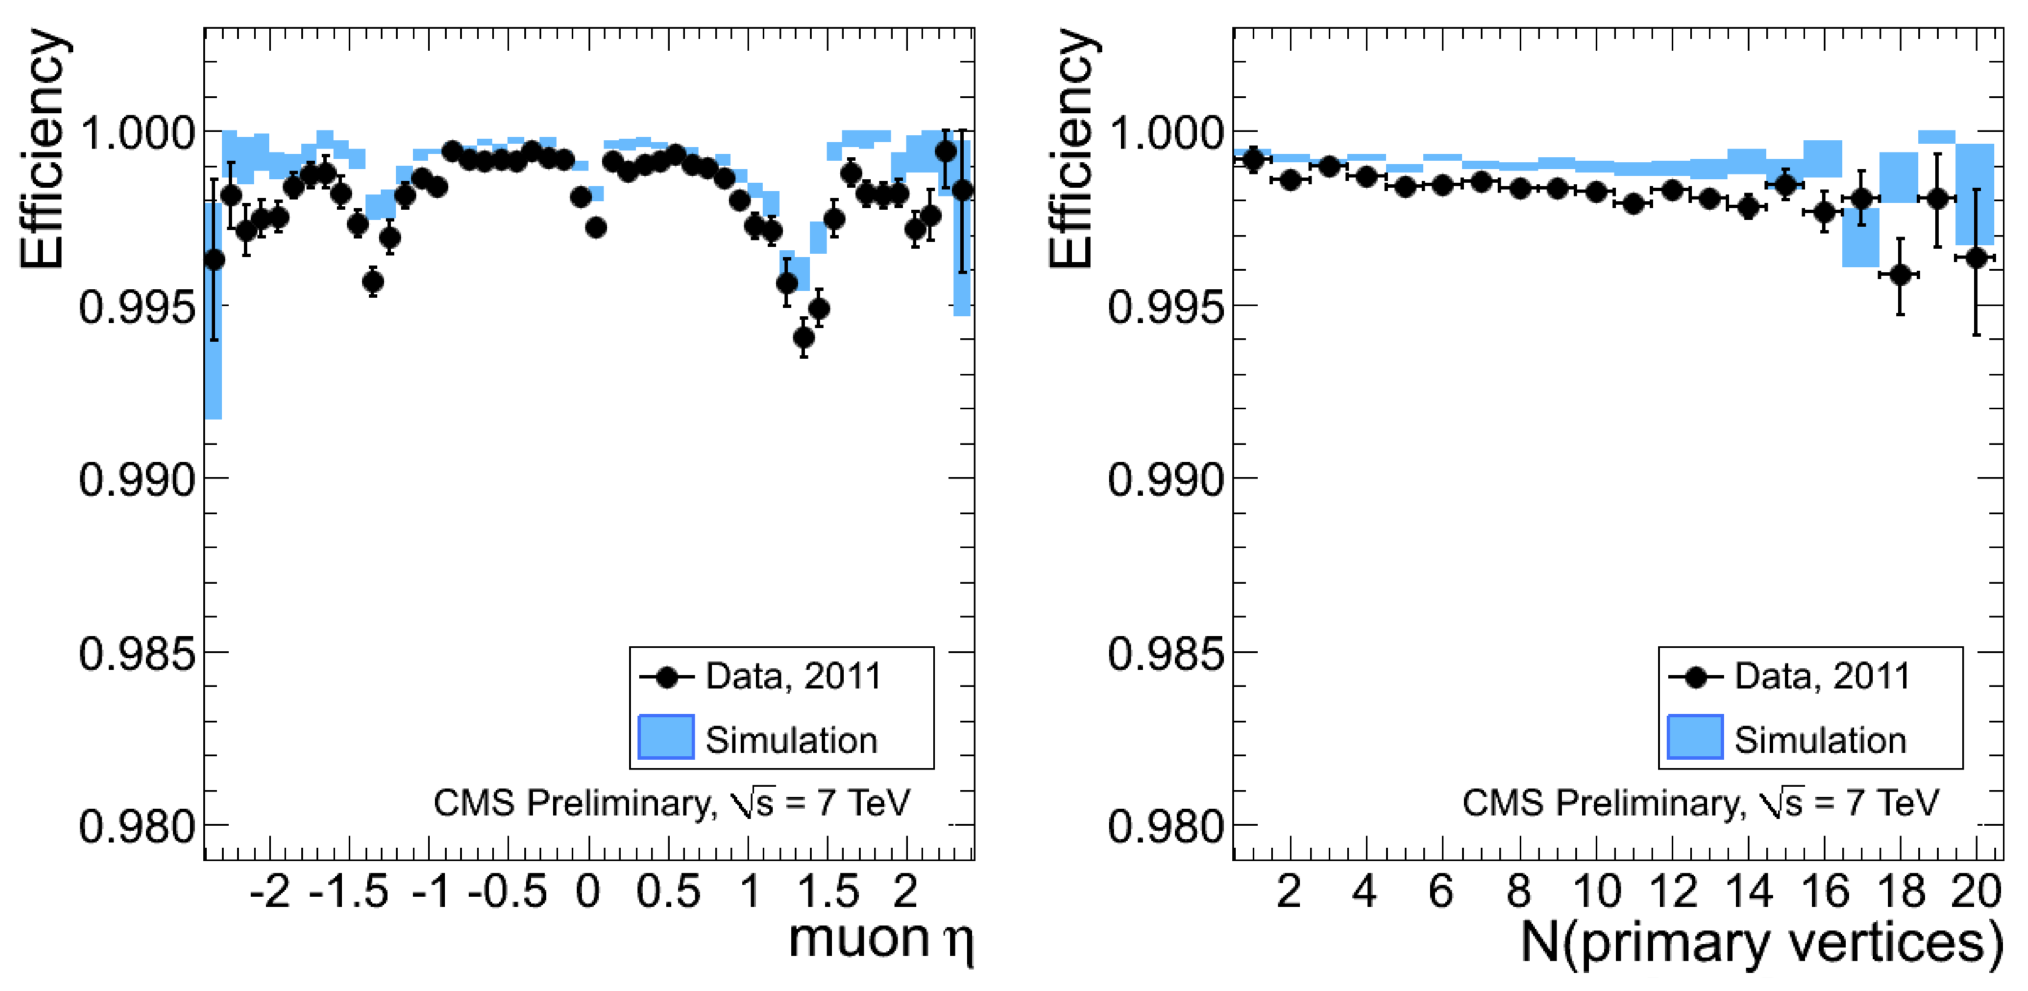
\includegraphics[width=0.9\textwidth]{figures/MuonTagAndProbeEfficiency.png} 
\end{tabular} 
\caption{Muon tracking efficiency in data and MC as a function of 
\Eta(left) and the number of reconstructed vertices(right)~\cite{muonTrkPerform}. 
The agreement between data and MC is at the level of a few permille.} 
\label{fig:TrackingEffData} 
\end{figure} 



%\textcolor{blue}{ 
%Using the obtained seeds, Kalman filter \cite{} is used to find tracks. 
%The Kalman filter generates a tree of track candidates ... 
%Staring from innermost strip layer, the filter continues all the way to the 
%outermost layer ... \textcolor{red}{fill me}.
%At each step of track finding, the track state vector, 
%the momementum, direction, position of at the given surface, is carried 
%with covaricance matrix to the state vector. 
%The filter is composed of propagation and update steps which proceed 
%alternatively at each layer. In the propagation step, the track state 
%at the current surface is propagated to the next surface with the covariace 
%matrix which used linear error propagation. The covariance matrix includes 
%the effects of materials that the track should cross to reach the next surface. 
%The effects of Multiple Coulomb scattering as well as \brem\ for electrons 
%are added to the covariance matrix. The momemtum is subtacted by the mean of energy 
%loss and the variance of the energy loss distribution is added to the the variance 
%of momentum.  In the update step, the propagated state from the previous surface 
%is combined with the measurement of the currect surface. }


%%%%%%%%%%%%%%%%%%%%%%%%%%%%%%%%%%%%%%%%%%%%%%%%%%%%%%%%%%%%%%%%%%
\section{ Event Primary Vertex }

The primary vertex, the space point where a hard interaction takes place,
is reconstructed using the reconstructed tracks described in the previous section. 
The tracks are selected based on 
\begin{itemize}
\item compatibility with interaction region : the transverse impact parameter 
      significance with respect to the beamline should be less than 5, 
\item number of hits in the tracker : more than 4(2) hits should be 
      in the silicon strips(pixel detector) 
\item track fit quality : $\chi^2/\textrm{ndof}$ should be less than 20.
\end{itemize}
The selected tracks are clustered using the Deterministic Annealing 
algorithm~\cite{DAclustering}.
At first, only is used the z information at the point of the closest approach(PCA) with 
respect to the beem line. 
% look at http://cmssw.cvs.cern.ch/cgi-bin/cmssw.cgi/CMSSW/RecoVertex/PrimaryVertexProducer/python/OfflinePrimaryVerticesDA_cfi.py?revision=1.8&view=markup
% It says : distance of closest approach < 5sig, #hits >=5(2) for silicon(pixel), chi2/ndf < 5
Then, an adaptive vertex fit~\cite{AdaptiveVertexFit} is performed using the clustered tracks 
for each primary vertex
which has at least two associated tracks. The fit calculates the best estimates 
of the vertex parameters such as position and covariant matrices. 
The vertex is retained if the distance between the vertex and the beam line 
is less than 1~\cm.
%In case there is less than two tracks beam spot is used as a primary vertex. 

Fig.~\ref{fig:VtxEff} shows the vertex reconstruction efficiency as a function 
of number of tracks($N_{track}$) for data and simulation, 
and the transverse in the x direction and the longitudinal vertex resolution 
as a function of $N_{track}$ in the jet-enriched data and the min-bias data. 
%https://twiki.cern.ch/twiki/pub/CMSPublic/PhysicsResultsTRK/20120911_TRKPOG_Plots_Vertex2012.pdf
The recontruction efficiency is close to 100~\% with  
$N_{track}>2$. The transverse and londitudinal resolutions measured with 
the min-bias data are less than 30 and 40~\um, repectively, with $N_{track}=30$.
%For the \mHi=125~\GeV\ events, the average number of tracks per reconstructed 
%vertex is about 30, and about 100~\% of events have more than 10 tracks for 
%a vertex. So, for the signal events, the vertex reconstruction efficiency 
%is expected to be 100~\% and the resolution is less than ...  
% CAUTION : when mention this, note that the vertex eff can be different 
% in the QCD and HWW events

\begin{figure}[htp] 
\centering 
\begin{tabular}{c} 
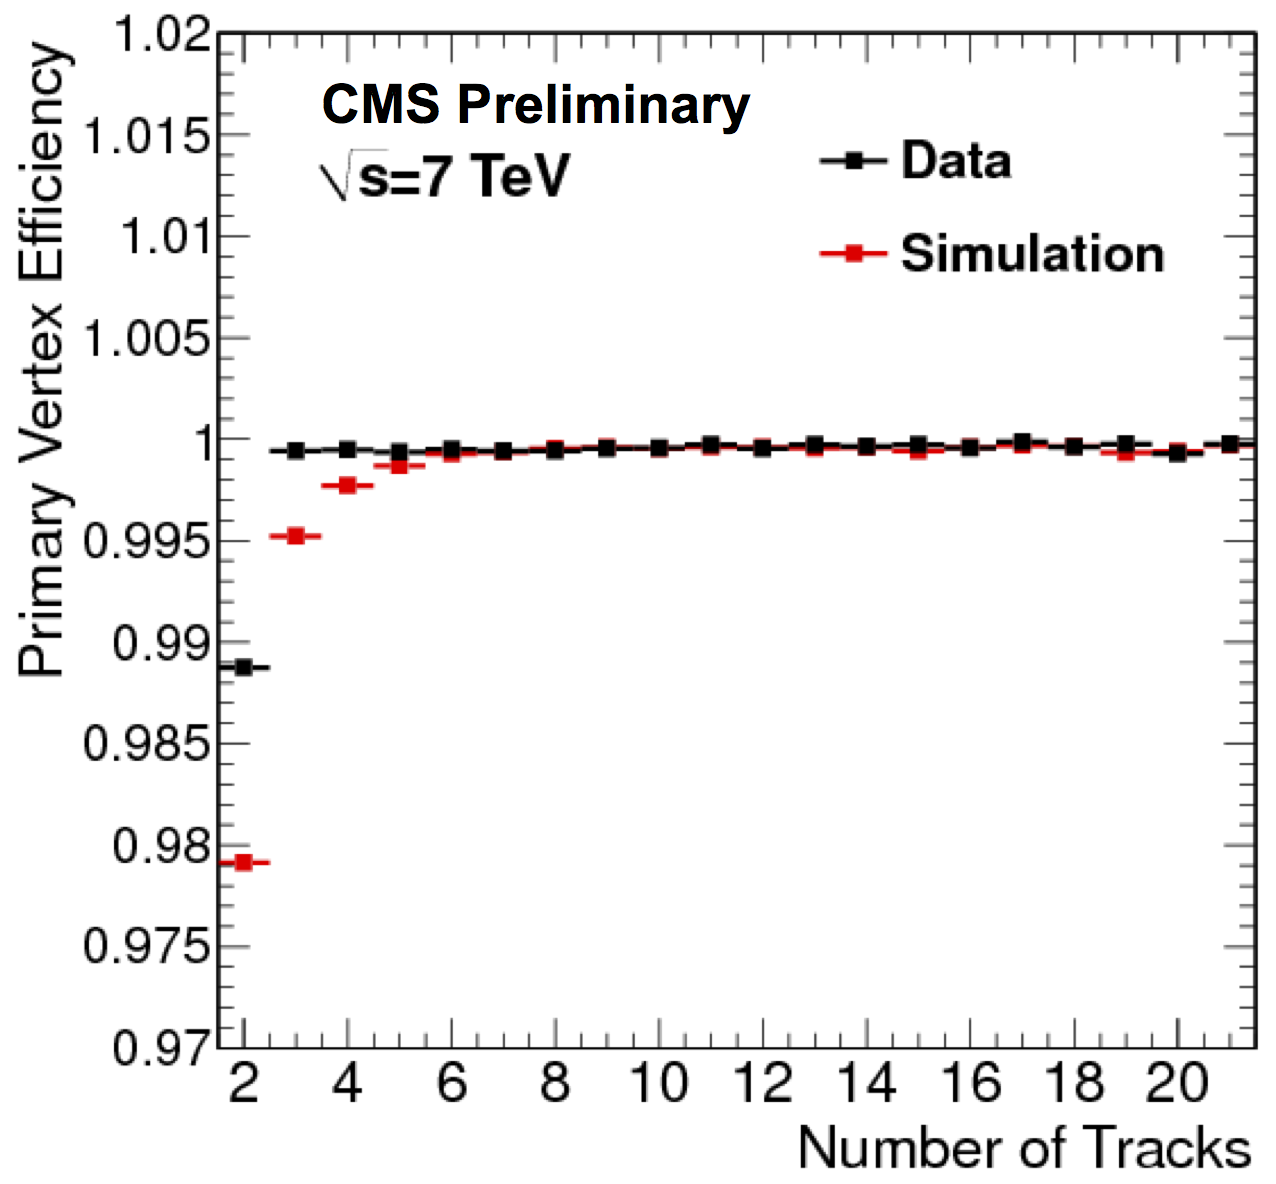
\includegraphics[width=0.45\textwidth]{figures/PrimaryVertexTagAndProbeEfficiency.png} \\ 
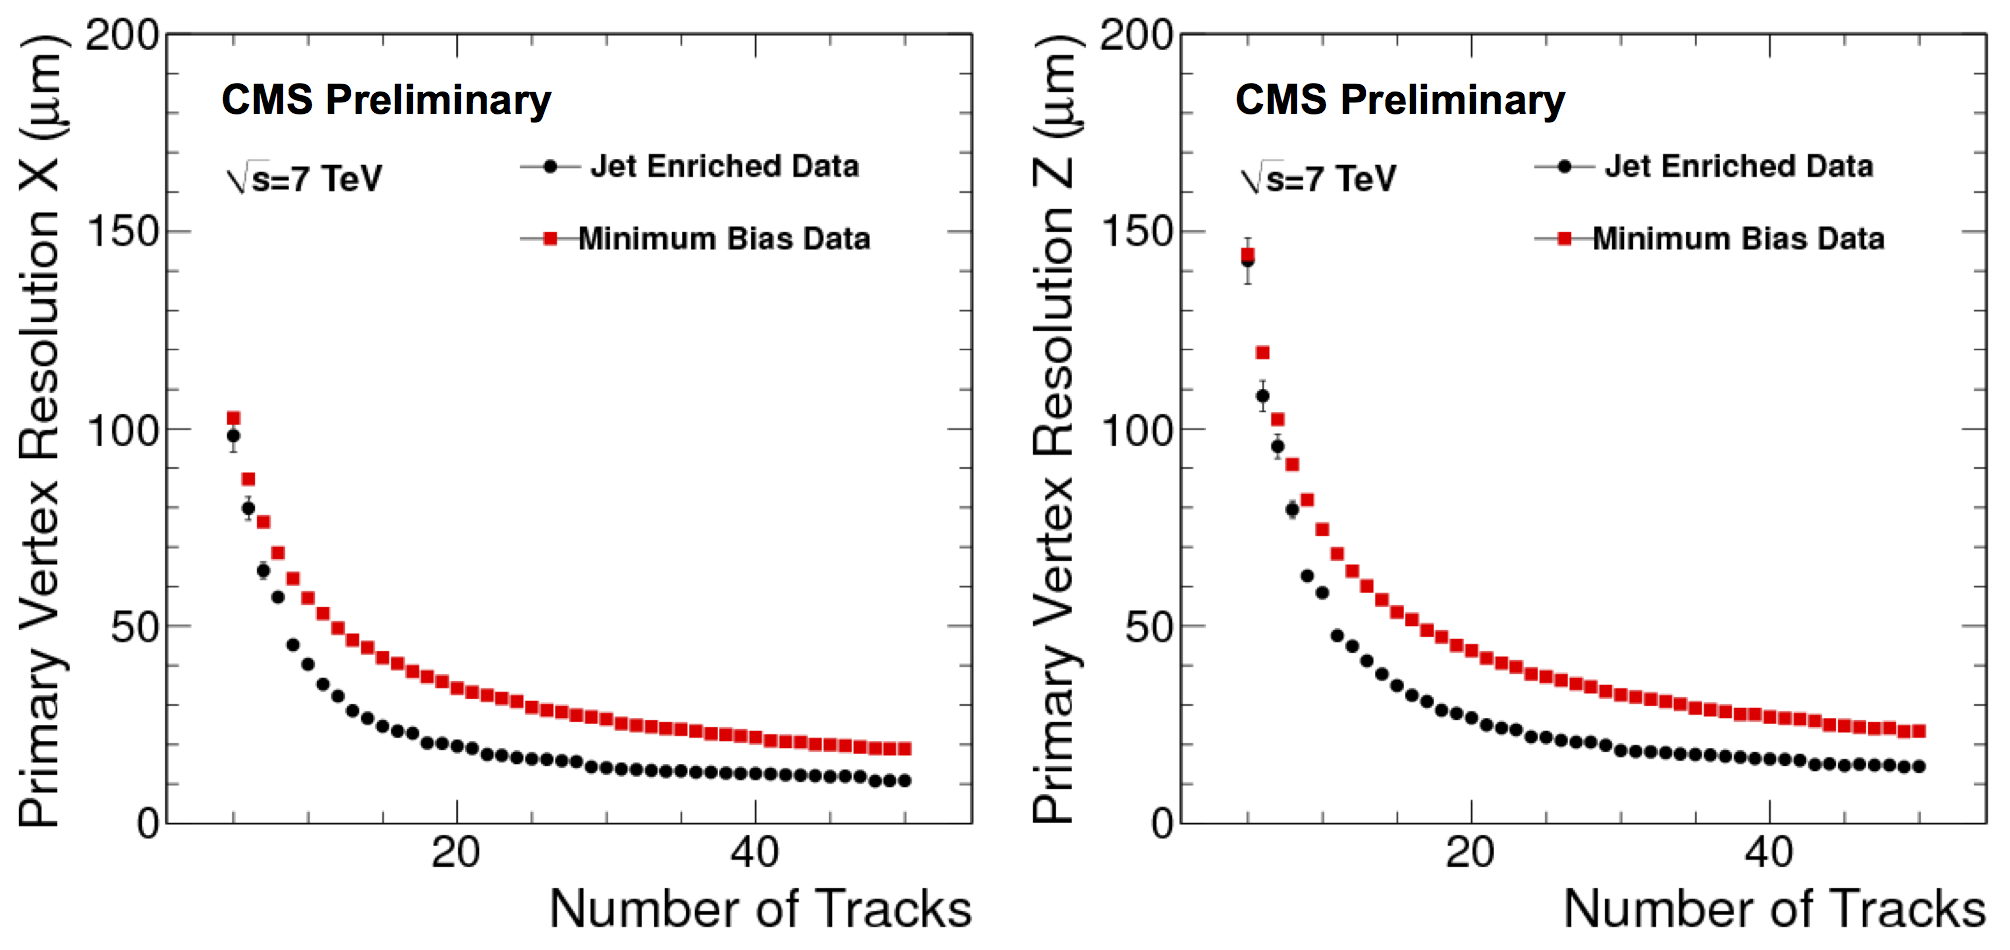
\includegraphics[width=0.9\textwidth]{figures/PrimaryVertexResolutions.png}  
\end{tabular} 
\caption{The vertex resolution in x and z directions as a function of associated tracks
for data and Simulation at the top 
and the vertex reconstuction efficiency as a function of number of associated tracks
for jet-enriched data and min-bias data at the bottom~\cite{muonTrkPerform}. }
\label{fig:VtxEff} 
\end{figure} 
%$root /hadoop/cms/store/user/jaehyeok/CMS2_V05-03-28/GluGluToHToWWTo2LAndTau2Nu_M-125_8TeV-powheg-pythia6_Summer12_DR53X-PU_S10_START53_V7A-v1/ntuple_10_1_hON.root
%root[] Events.Draw("trks_trk_p4@.size()/evt_nvtxs","trks_trk_p4@.size()/evt_nvtxs>10")

%%%%%%%%%%%%%%%%%%%%%%%%%%%%%%%%%%%%%%%%%%%%%%%%%%%%%%%%%%%%%%%%%%
\section{ Electron }
\label{sec:electron_reco}
%\textcolor{red}{How is the location of electron calculated !!}

Electrons are reconstructed using the information from the tracker and the ECAL 
because an electron makes hits in the tracker and makes energy deposit in the ECAL.
To reconstruct an electron, ECAL clustering is done first to collect energy 
spread including \brem(the collection is called ``supercluster"), 
and the track reconstruction is performed using a pixel seed found 
by the supercluster-driven method~\cite{Baffioni:2006cd}.  
 
The electrons and photons radiated off the electrons 
form an electromagnetic shower, and make their energy deposit in the ECAL. 
%A test beam result~\cite{Baffioni:2006cd} shows that for a single electron 
%in barrel of an energy 120~\GeV, 97 \%  of its energy is stored in a 
%$5\times5$ crystal cluster. 
But, when an electron travels in the tracker which is placed in a strong magnetic field, 
it radiates photons by \brem, and the energy deposit 
in the ECAL has a spread in the $\phi$ direction. The size of the energy loss due to \brem\ 
is significant enough to be included for electron energy calculation. 
For example, for electrons of energy 10, 30 and 50~\GeV, about 35 \% of electrons 
lose more than 70 \% of their initial energy via \brem, and about 10 \% of them 
lose more than 95 \%~\cite{Baffioni:2006cd}. Therefore, in order to 
obtain the initial electron energy, it is critical to collect all \brem\ photons.
The algorithm for this purpose is called super-clustering algorithm~\cite{Baffioni:2006cd}.

The CMS employs two algorithms, hybrid for barrel region 
and island for endcap region~\cite{Baffioni:2006cd}. 
The hybrid algorithm forms a domino of 3 or 5 crytals in \Eta, and
dynamically searches for dominos in $\phi$ separated by a domino with energy less 
than 100~\MeV.
The island algorithm starts with making a cluster from a seed crystal with energy deposit 
above a cerntain threshold, and collect crystals around it 
in $\phi$ and then $\eta$ direction. 
The resultant clusters in narrow $\eta$-window and wider $\phi$-window 
are then used to construct a supercluster.

The position of the shower($x$) is measured as a weighted mean of position of crystals 
in a cluster~\cite{cmstdr1}. 
\begin{eqnarray} 
x = \frac{\displaystyle \sum_i^{N_{crystals}} {x_i} \cdot \omega_i}
         {\displaystyle \sum_i \omega_i}   
\end{eqnarray}
where $x_i$ is the position of the crystal $i$, 
and $\omega_i$ is the weight for the crystal $i$ given by  
\begin{eqnarray} 
\omega_i = \omega_0 + \log{\frac{E_i}{\displaystyle \sum_j E_j}}.
\end{eqnarray} 
The logarithmic form of the weight is motivated by the fact that 
the energy density decreases exponentially in the lateral direction 
from the shower core.  

Once the energy is collected, electron tracks are reconstructed. The first step is 
to generate seeds to start the tracking algorithm. The energy-weighted mean 
supercluster position is extrapolated to the interaction point(beam spot) 
to find compatible hits in the pixel detector assuming both charge hypotheses. 
The innermost layer is looked for first with loose $\Delta\phi$ and $\Delta z$ window. 
If compatible hits are not found in the first layer, search goes on to the next layer. 
If a compatible hit is found, the z coordiate of the primary vertex is calculated,
and the predicted trajectory is used to find compatible hit(s) in the next pixel layer(s).  
Using the selected seed, compatible hits in the next silicon layer are looked for,  
and extrapolation is done to the next layer using Beath-Heitler modeling of electron 
\brem~\cite{BetheHeitler} 
and Gaussian Sum Filter(GSF) \cite{0954-3899-31-9-N01} which assumes that the \textit{pdf} 
of the Bethe-Heitler model is a Gaussian mixture. 
The procedure is continued to the last layer unless two consecutive hits are not found. 
At each layer, the trajectory state is updated using the weighed mean of the measurement 
and the prediction. When there are multiple compatible hits, the two most compatible ones 
from $\chi^2$ test are kept. Finally, a track is created if there are at least five hits. 

Fig.~\ref{fig:ElectronEnergyResMC} shows the resolution of reconstructed electron energy 
as a function of the true electron energy measured with simulation~\cite{PAS-HIG-13-002}.   
As shown in the figure, precision is dominated by the information 
from the tracker(blue reverse trianle) and the ECAL(green upright triangle) 
at low and high energy, respectively. 
The final resolution comes from the combination of the information weighted by 
their errors(red star). These errors are evaluated by the half minimum width that 
contains 68.3\%(Gaussian 1$\sigma$ width) in the energy distribution. 
The red circle corresponds to the width of the Guassian fit in the core of the 
energy distribution. 

\begin{figure}[htp] 
\centering 
\begin{tabular}{c} 
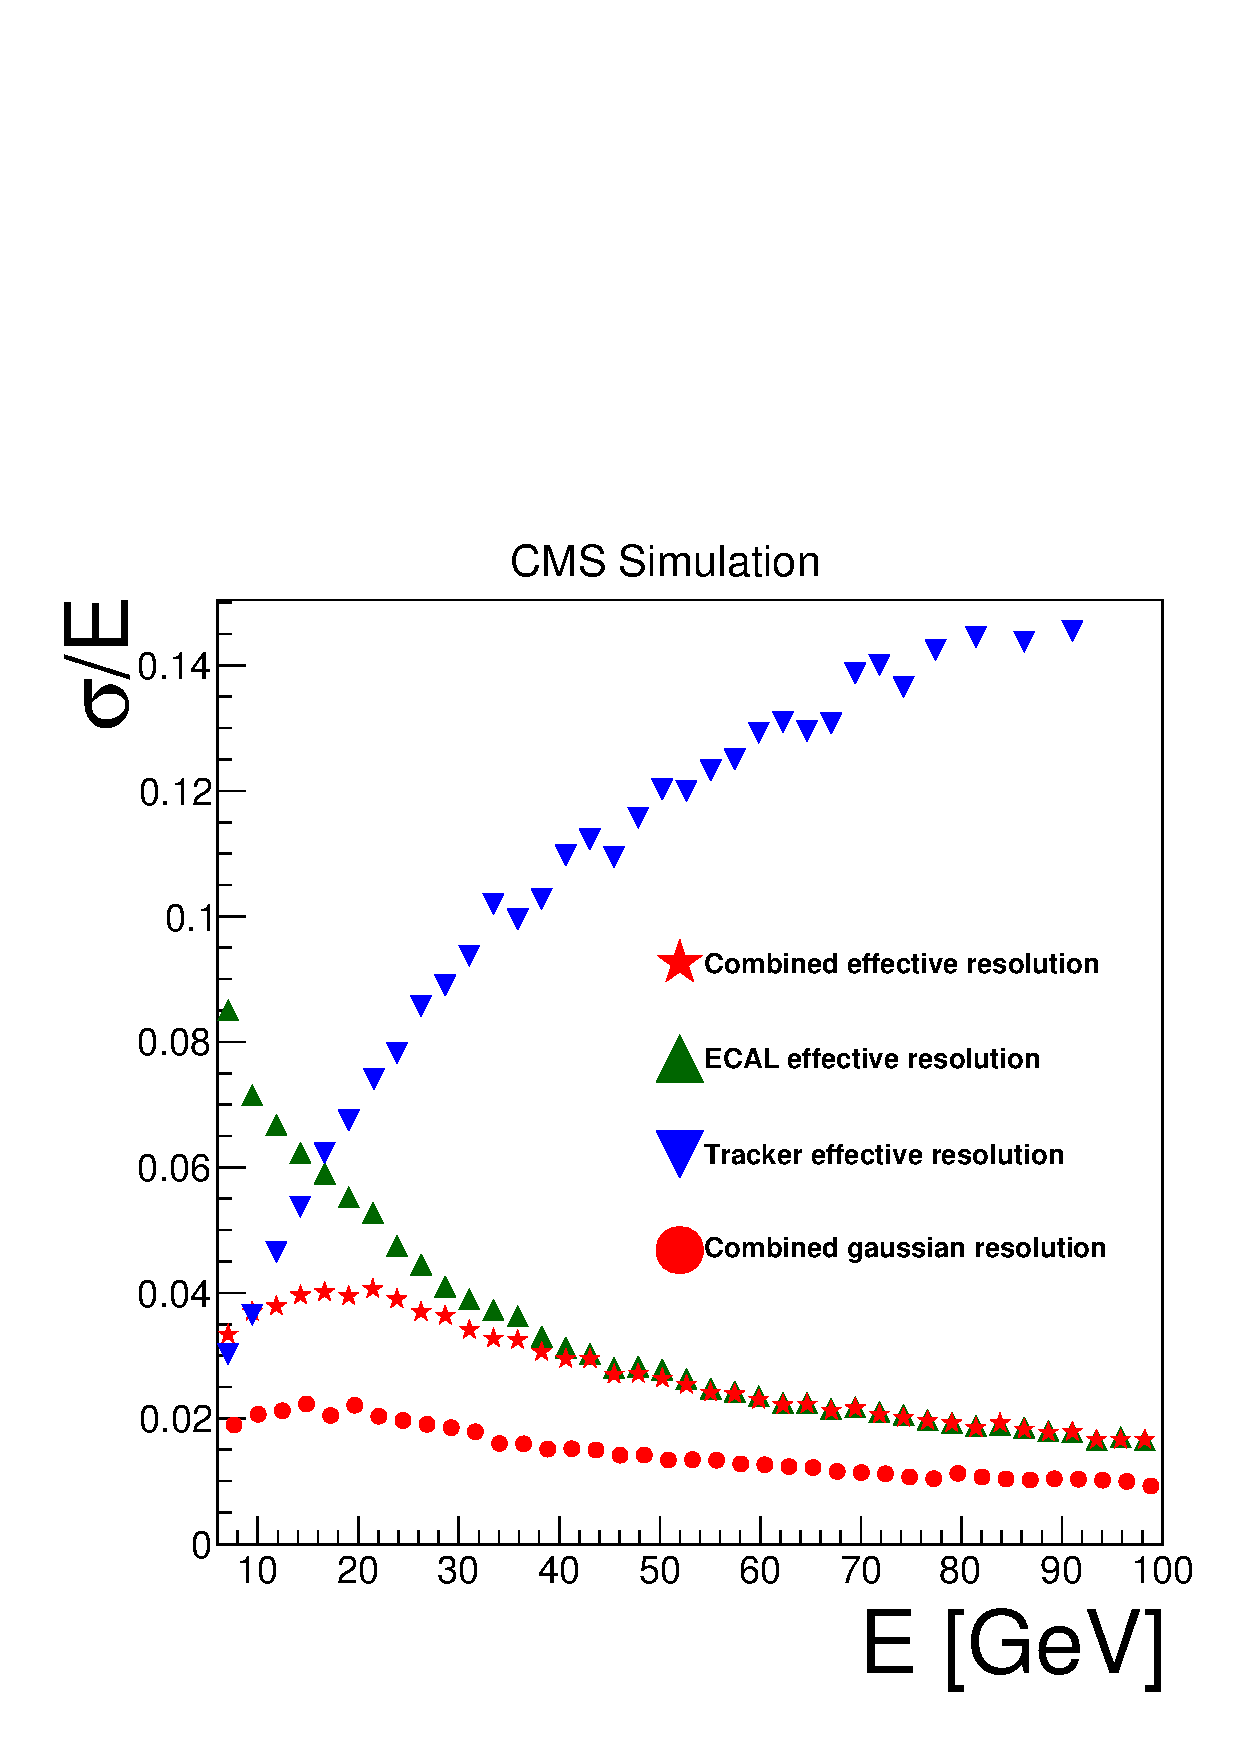
\includegraphics[width=0.6\textwidth]{figures/effRMSfinal-3.pdf} 
\end{tabular} 
\caption{Energy resolution of reconstructed electrons as a function 
of generated electron energy from different information 
in simulation~\cite{PAS-HIG-13-002}. 
Blue reverse triangle is measured using only tracker information 
and green upright triangle is measured using only ECAL information. 
The red star is a combination of the tracker and ECAL measurments. 
The resolution is estimated the half minimum width that
contains 68.3\%(Gaussian 1$\sigma$ width) in the energy distribution
as denoted as effective resolution. The red circle corresponds to the 
width of Guassian fit in the core of the energy distribution.
}
\label{fig:ElectronEnergyResMC} 
\end{figure} 

%%%%%%%%%%%%%%%%%%%%%%%%%%%%%%%%%%%%%%%%%%%%%%%%%%%%%%%%%%%%%%%%%%
\section{ Muon }
\label{sec:muon_reco}

In CMS there are three types of muons depending on the information used in the 
reconstruction~\cite{cmstdr1}. They are standalone, traker and global muons.   

The \textit{Standalone} muon reconstruction uses information from 
the muon system(DT, CSC and RPC), \textit{i.e.} the inner tracker information is not used. 
It starts with the reconstruction of the track segments in the muon chambers. 
The digitized electronic signals in DT, CSC and RPC are used to 
reconstruct hits. Then, the hits in DT and CSC are matched to form the segments. 
The information of these segments, such as momentum, at the innermost 
muon chamber is used as a seed to construct a muon track using the Kalman-filter 
algorithm. The Kalman-filter is an iterative algorithm 
that updates the track parameters iteratively as it goes to the next station. 
At each step of the track parameters estimation, if no matching segment is found 
then the search continues to the next station taking into account the detector 
effects such as multiple scattering and energy loss in the material. 
The procedure goes until the outermost station, updating the track parameters 
at each step. Then, the Kalman-filter is applied from the outermost to 
the innermost station, and the track parameters are defined at the innermost 
station. Finally, the measured muon track is extaploated to the interaction 
point and a vertex-constrained fit is performed to obtain the final track parameters. 

The \textit{Tracker} muon reconstruction uses information from  
the inner tracker, \textit{i.e.} the muon system information is not used
for the momentum measurement. This approach considers all tracks as 
potential muon candidates, and checks their compatibility with the 
muon system. All tracker tracks with $\pt>0.5~\GeV$ and $p>2.5~\GeV$ 
are extrapolated to the muon system considering the expected detector effects 
such as magnetic field, multiple scattering and energy loss in the material. 
If there is at least one muon segment matched to the 
extrapolated track, this muon is considered as a Tracker muon. 
The tracker muon gives good momentum measurement and identification 
for the low \pt\ muons which are hard to be reconsructed by the muon system
because they do not leave enough track segments in the muon system. 

The \textit{Global} muon reconstruction uses information from both the tracker 
and the muon system. For a standalone muon track obtained by the way explained 
already, a matching with a tracker track is done. 
The muon track at the innermost station is extrapolated to the last layer 
of the tracker considering the expected detector effects.
If the matching is successful, the Kalman-filter is used to reconstruct the tracks. 
After that, all reconstructed tracks are fitted again without constraints on the 
beamspot, using the hits associated with the standalone muons and the hits 
in the silicon strips. A fit is done again using the tracker hits and the 
hits in the innermost muon station, and the fit quality is compared with 
that of the tracker-only fit. This is to detect muon \brem\  or 
any loss of energy before reaching the muon station.

In summary, there are three approaches for muon reconstruction in CMS. 
Having multiple algorithms provides more reliable muon reconstruction, 
and physics analysis can choose algorithms of their interests. 
\begin{figure}[!hbtp]
\centering
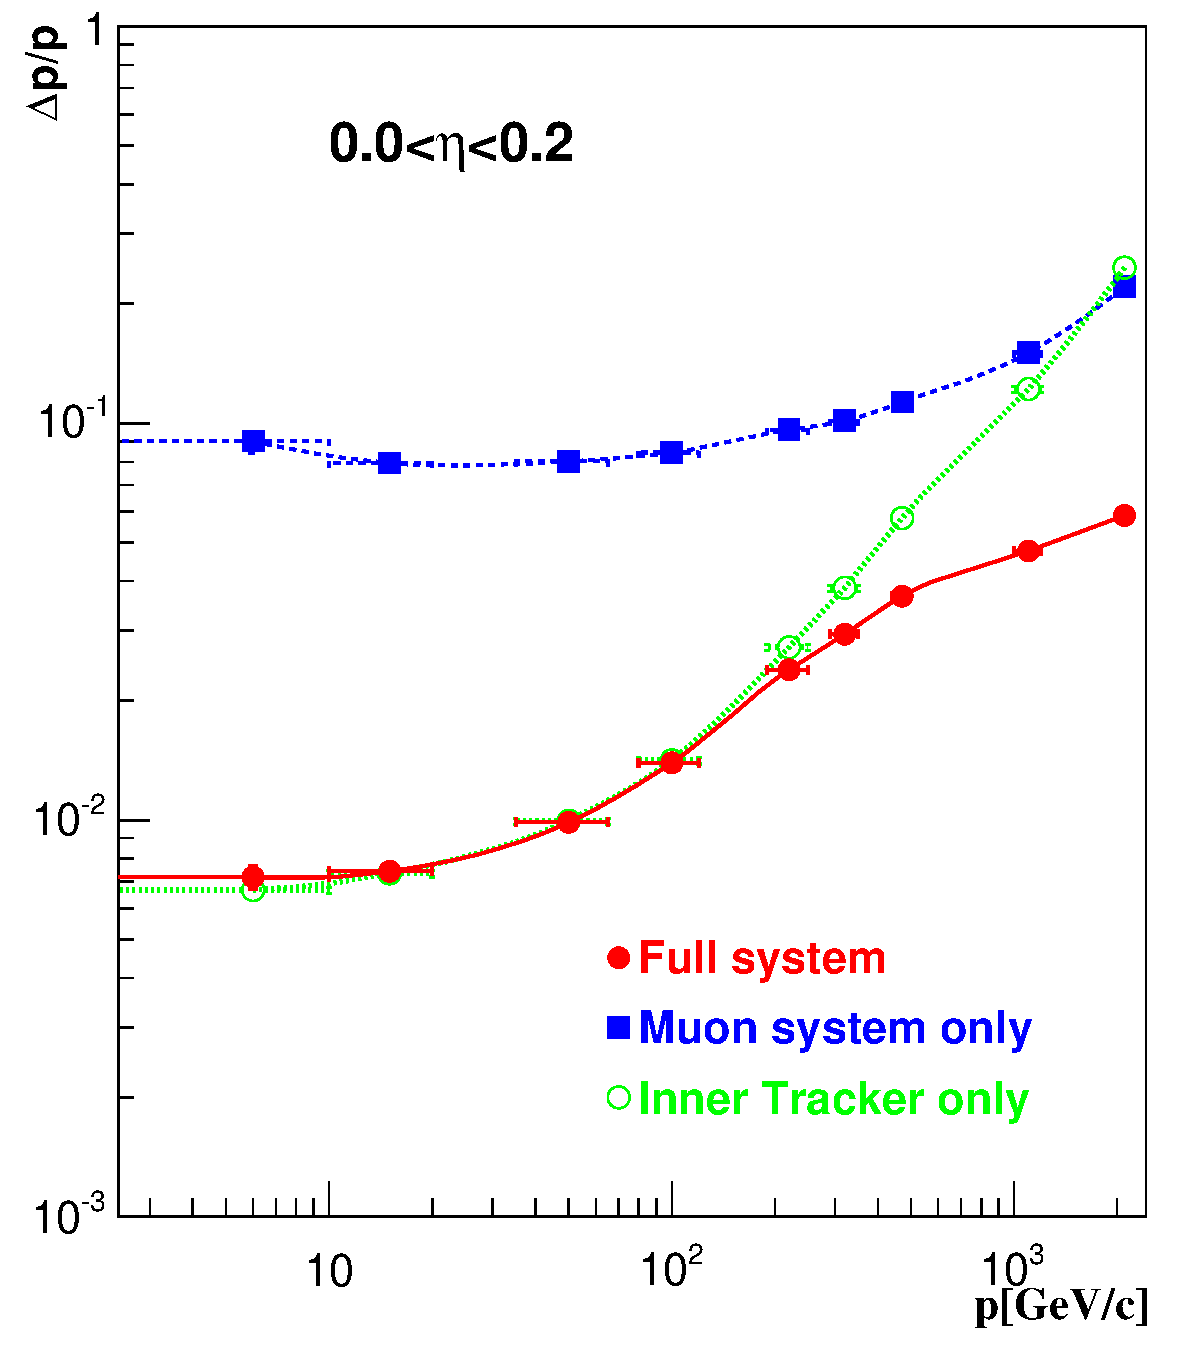
\includegraphics[width=.45\textwidth]{figures/Figure_001-005-a.pdf}
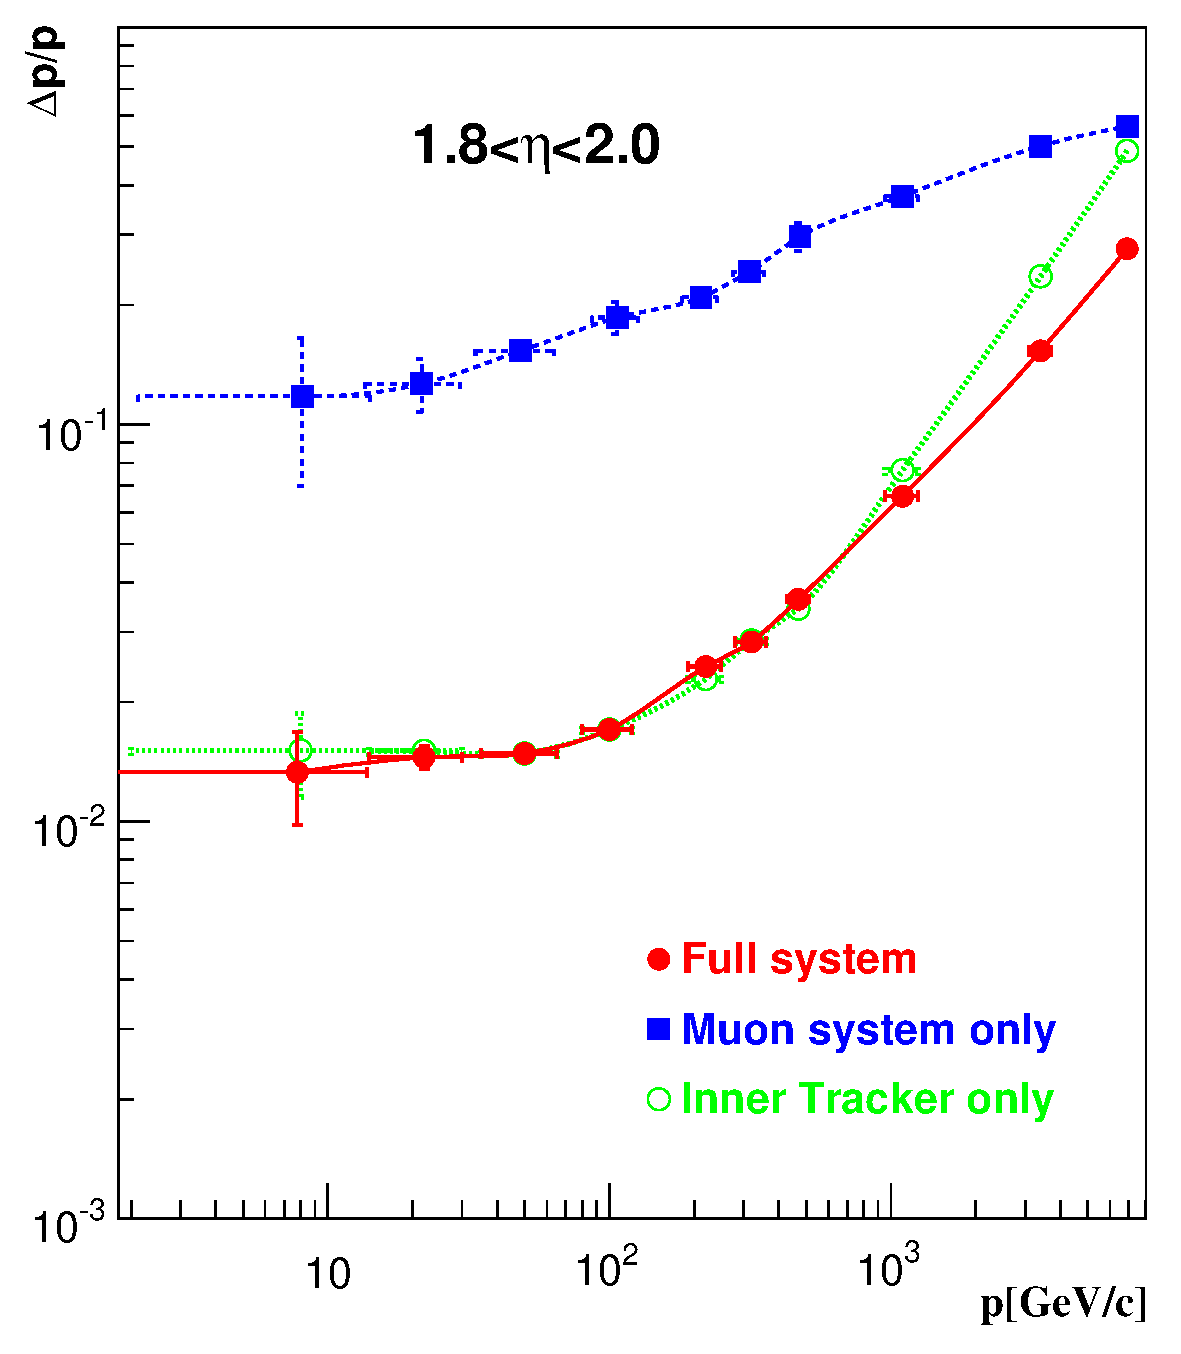
\includegraphics[width=.45\textwidth]{figures/Figure_001-005-b.pdf}
\caption{Resolution of muon momemtun in $0.0<|\eta|<0.2$ and $1.8<|\eta|<2.0$. 
Red, blue and green are global, standalone and tracker muons, 
respectively~\cite{cmstdr1}.} 
\label{fig:muon_res}
\end{figure}
Fig.~\ref{fig:muon_res} shows the momentum resolution of difference muon 
reconstruction algorithms as a function of muon \pt\ 
in the barrel(left) and endcap(right)~\cite{cmstdr1}. 
The resolution of standalone muons is dominated by mutiple scattering in the material 
before the muon station at $\pt<200~\GeV$  and by the spacial resolution 
of the muon chambers at $\pt>200~\GeV$. The tracker muons give much better 
resolution at low \pt\, but the resolution goes up to the same level 
with the stanalone muons at very high \pt. For muons with $\pt<200~\GeV$, 
the resolution is better than 3~\%.

%%%%%%%%%%%%%%%%%%%%%%%%%%%%%%%%%%%%%%%%%%%%%%%%%%%%%%%%%%%%%%%%%%
\section{ Jet }
\label{sec:jet_reco}
%\begin{itemize}
%\item \textcolor{red}{Jet reconstruction : anti-kT (dR = 0.5) }
%\item \textcolor{red}{Jet energy correction : L1Fastjet/L2/L3 (+ Residual correction in data) }
%\end{itemize}

The existence of gluons and quarks in the event is manifested as a hadronic shower, 
``jets", which leaves an energy deposit primarily in the HCAL. 
Thanks to the fine granuality of the caloremeters and high precision of tracking in CMS, 
individual stable particles(electron, muon, photon, charged and neutral hadron) 
can be reconstructed by Particle-Flow(PF) algorithm~\cite{PFalgo}. 
This algorithm uses all available information from sub-detectors 
to optimally determine the type of particles, momenta and energies. 
The reconstructed particles, PF candidates, are used to construct higher-level 
objects such as \met, jets, and b-tagging, etc.

The jets are reconstructed by clustering individual particles
that come from the same parton. The algorithm works 
such that the two distances are defined,
the distance between particle i and j($d_{ij}$) 
and the distance between particle i and the beam line($d_{iB}$). 
If the minimum of $d_{ij}$ and $d_{iB}$ is $d_{ij}$ then the two particles are merged,
and if the minimum is $d_{iB}$ then the paritle i is removed from 
the list of paricles because it is considered as a radiation from the beam. 
CMS uses anti-$\textrm{k}_\textrm{T}$ algorithm~\cite{Cacciari:2008gp}. 
In this algorithm, the distances are defined as 
\begin{eqnarray} 
d_{ij} 
&=&   
min \left( \frac{1}{k_{Ti}^2}, \frac{1}{k_{Tj}^2} \right) 
\frac{\Delta_{ij}^2}{R^2}, \\ 
d_{iB} 
&=&  
\frac{1}{k_{Ti}^2}
\end{eqnarray} 
where $k_{Ti}$ is the transverse momentum of particle $i$, 
$\Delta_{ij}^2 = \left( y_i - y_j \right)^2 + \left( \phi_i - \phi_j \right)^2$ 
with $y_i$ and $\phi_i$ being the rapidity and the azimuthal angle of particle $i$,
repectively, and $R$ is the scale that determines the distance of the reconstructed jets.   
CMS used $R = 0.5$ for the jet reconstruction. 
The clustering uses FastJet algorithm~\cite{Cacciari:2005hq} which
significantly improves the timing of calculation, and provides  
the jet area used for subtraction of contribution from PU. 

Due to the non-linear calorimeter response of the CMS detector, 
the measured jet energy can be different from the energy of the true parton which 
initiated the jet. The CMS employs a jet energy correction(JEC) 
method~\cite{Chatrchyan:1369486} factorized into multiple levels, 
the L1, L2, L3 and the residual L2L3 corrections for data as shown in fig.~\ref{fig:jec}. 
\begin{figure}[!hbtp]
\centering
\includegraphics[width=.95\textwidth]{figures/jec.pdf}
\caption{Factorized method for jet energy correction.}
\label{fig:jec}
\end{figure}

The L1 correction is the pileup correction, \textit{i.e.} to remove the offset energy 
produced by pileup. The correction factor($C_{L1}$) is defined by~\cite{Chatrchyan:1369486} 
\begin{eqnarray} 
C_{L1} = 1 - \frac{\left( \rho - \left<\rho_{UE+noise}\right>\right) \cdot A_{jet}}{p_T^{raw}}  \end{eqnarray} 
where $\rho$ is the per-event energy density, 
$\left<\rho_{UE+noise}\right>$ is the average energy density 
of Underlying Event(UE) and noise which is measured using events that contain only one 
reconstructed vertex, \textit{i.e.}, no PU, 
$A_{jet}$ is the jet area
and $p_T^{raw}$ is the uncorrected transverse momentum of the jet. 
The L2 correction is to make the jet energy response flat in \Eta.  
At a given \Eta\, the response is corrected so that it becomes the same level 
with the central region, $|\Eta|<1.3$. So, it is a relative correction.  
The correction factors are derived either from MC or using data-driven method
(di-jet balance technique~\cite{Chatrchyan:1369486}).
The L3 correction is to make the jet energy response flat in \pt.  
The central region, $|\Eta|<1.3$, is used as a referece for the correction. 
Apart from the L2 correction, L3 correction is an absolute correction 
such that the corrected jet \pt\ is same as the \pt\ of the parton that 
initiated the jet. The correction factors are derived either from MC 
or using data-driven method($Z/\gamma^*$+jet balance technique~\cite{Chatrchyan:1369486}). 
For L2 and L3 corrections, 
%the corrections based on MC truth is done for MC and 
residual corrections are applied to data in order to to account for the small differences 
between data and MC. 
% http://arxiv.org/pdf/1107.4277.pdf

Fig.~\ref{fig:jecuncert} shows the uncertainty on the JEC factor
as a function of jet \pt\ at $|\eta_{jet}|=0, 2.0, \textrm{ and }2.7$ 
They show that the uncertainty is less than 3~\% for jets with 
$\pt>30~\GeV$ at $|\eta_{jet}|=0 \textrm{ and } 2.0$. 
The uncertainty becomes larger in the forward region, 
\textit{e.g.} it is as large as 8~\% for jets with $\pt>30~\GeV$ at $|\eta_{jet}|=2.7$.  


\begin{figure}[!hbtp]
\centering
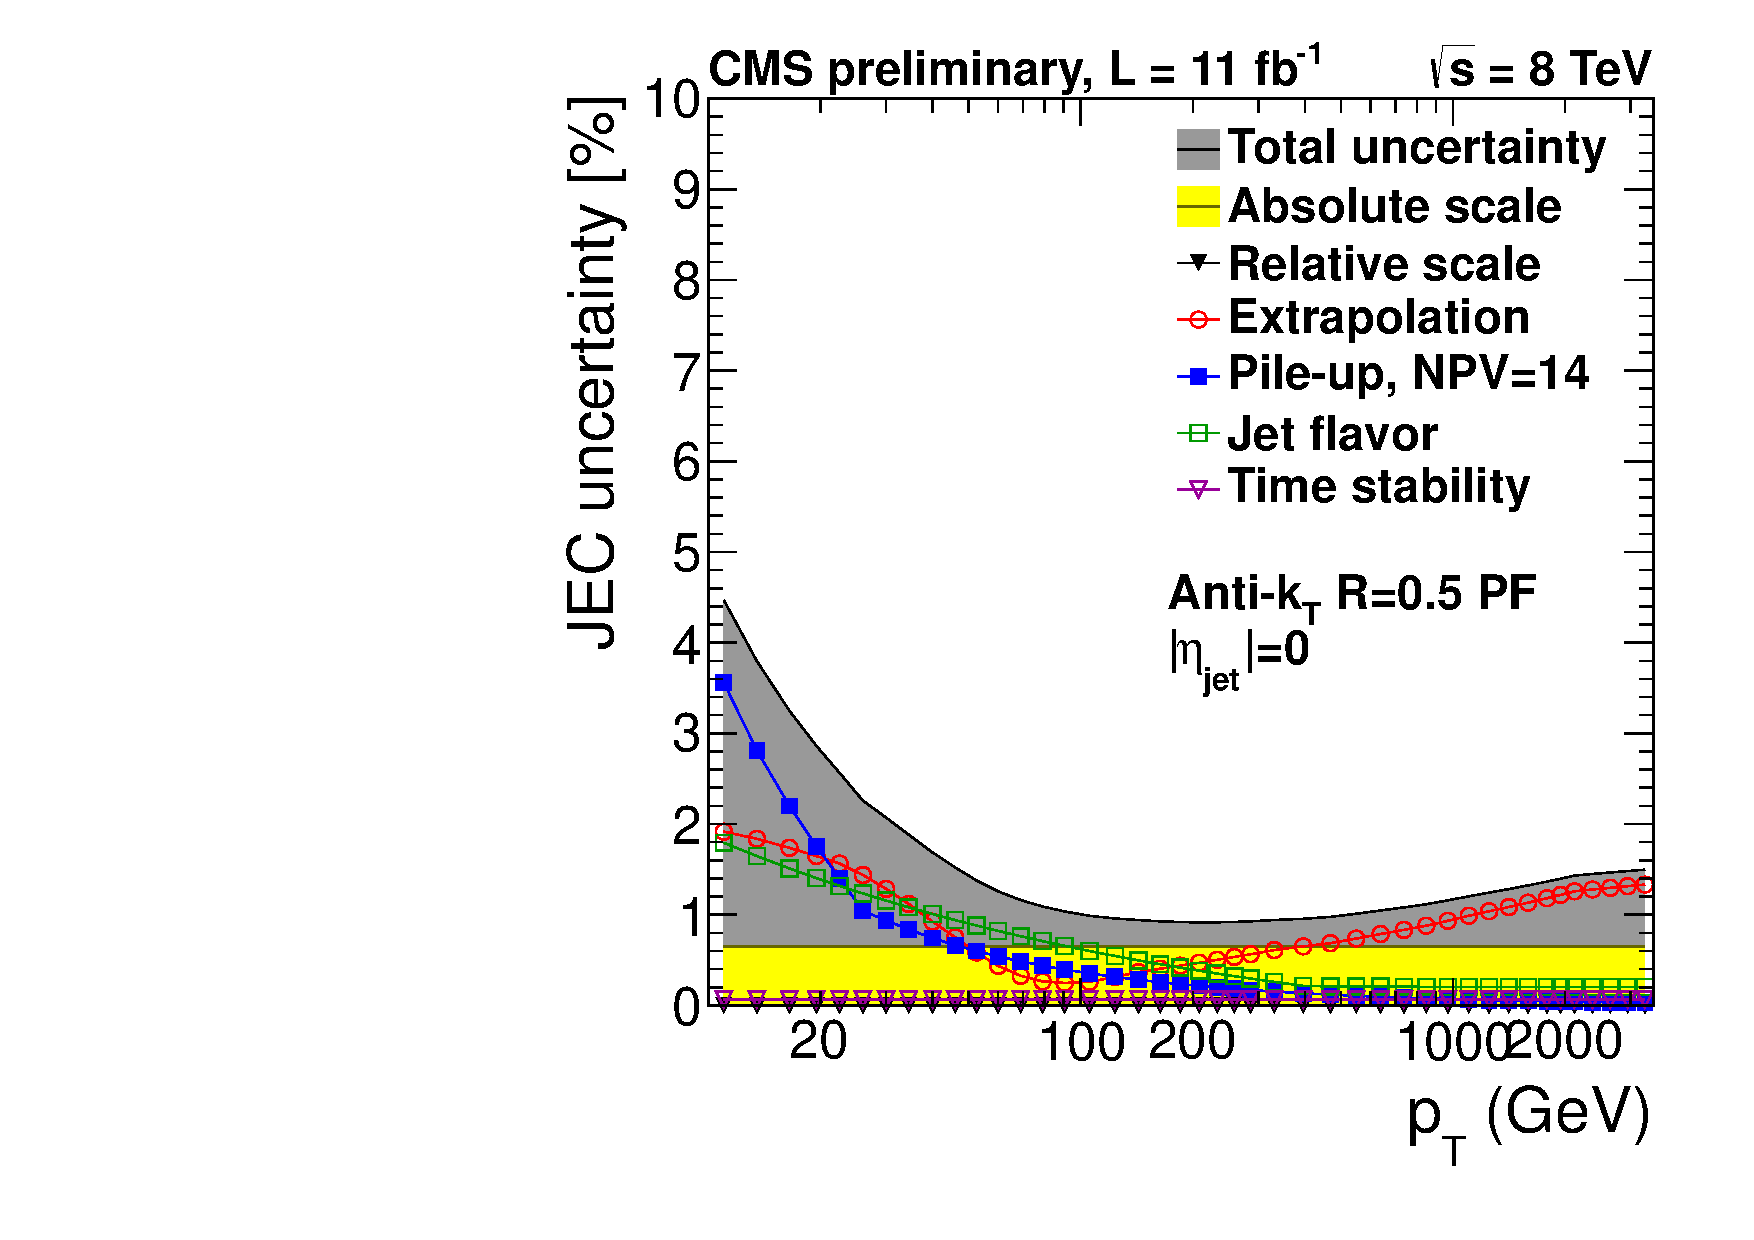
\includegraphics[width=.45\textwidth]{figures/JECUncert_Fall12_DATA_AK5PF_Eta00.pdf}
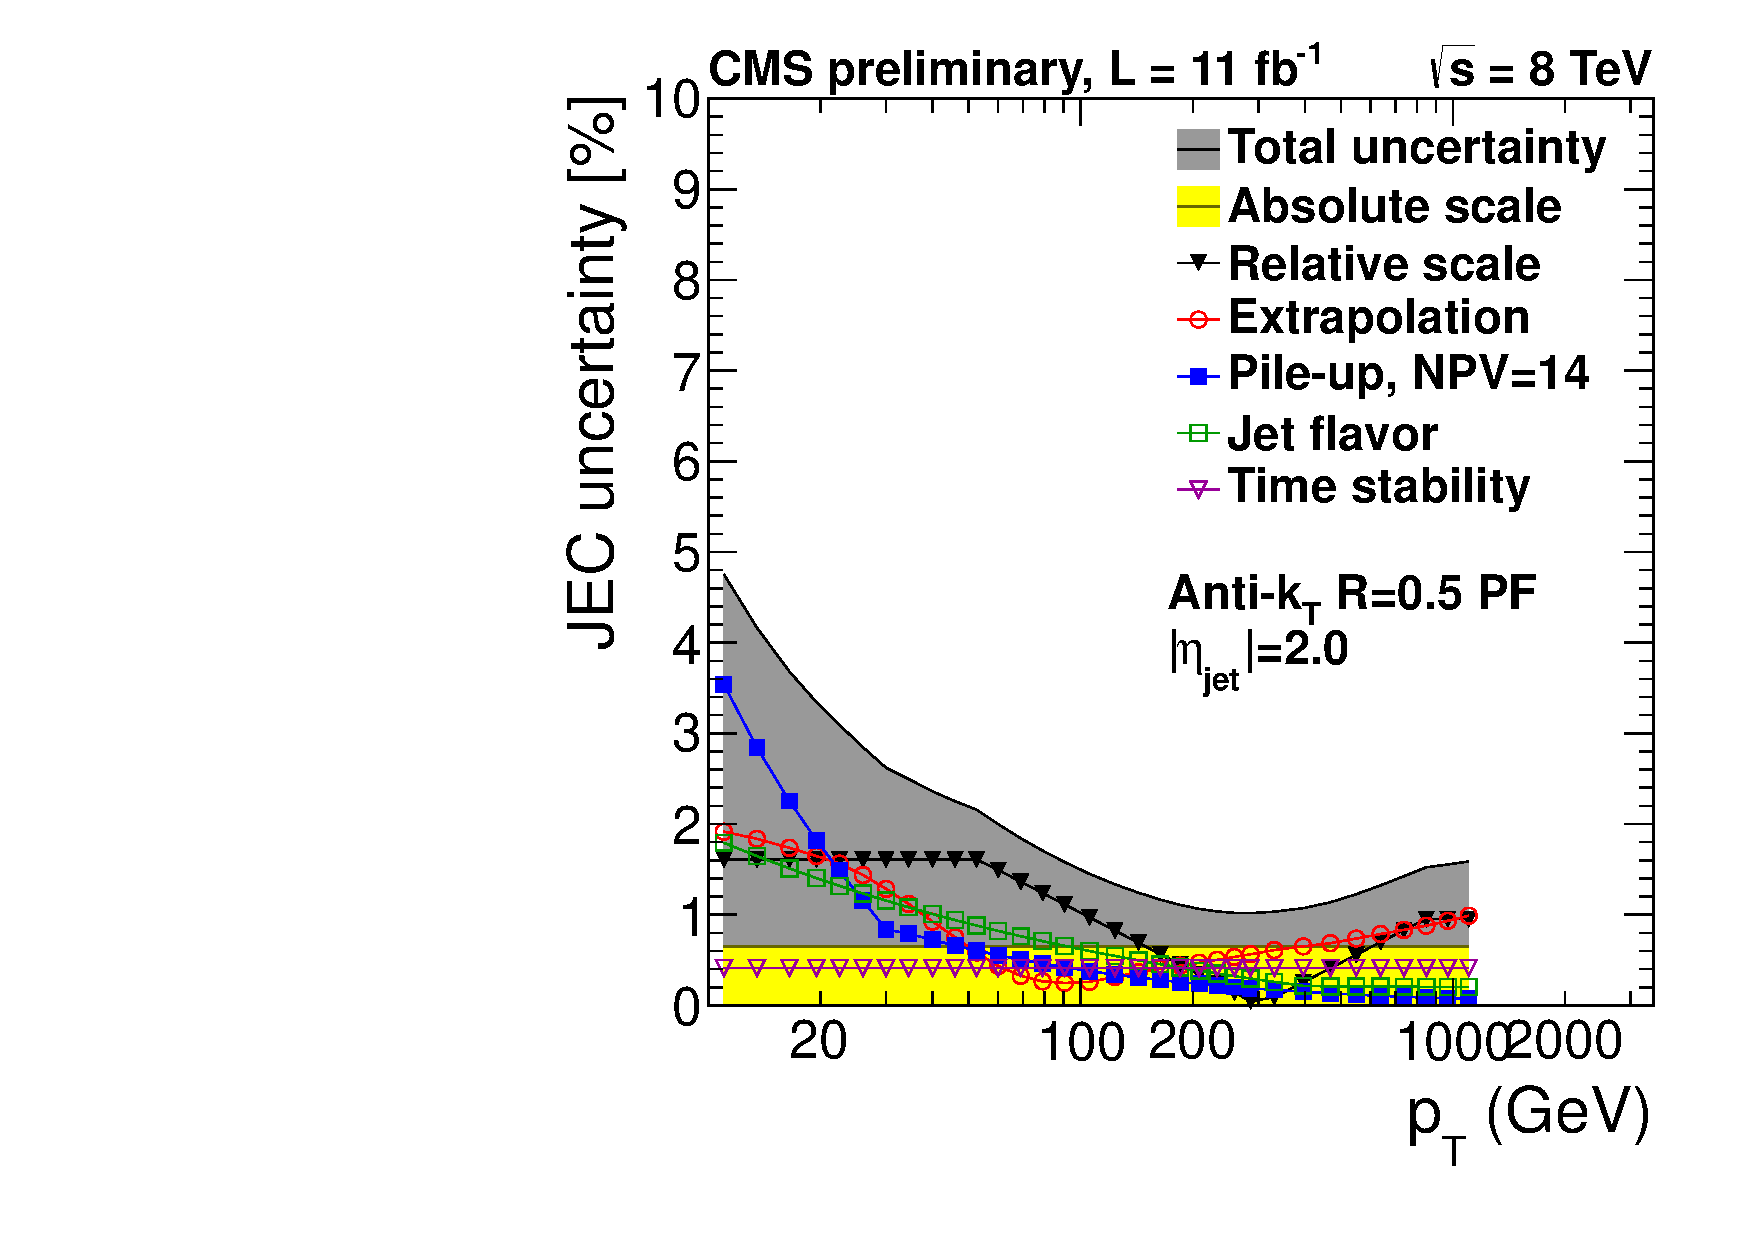
\includegraphics[width=.45\textwidth]{figures/JECUncert_Fall12_DATA_AK5PF_Eta20.pdf} \\
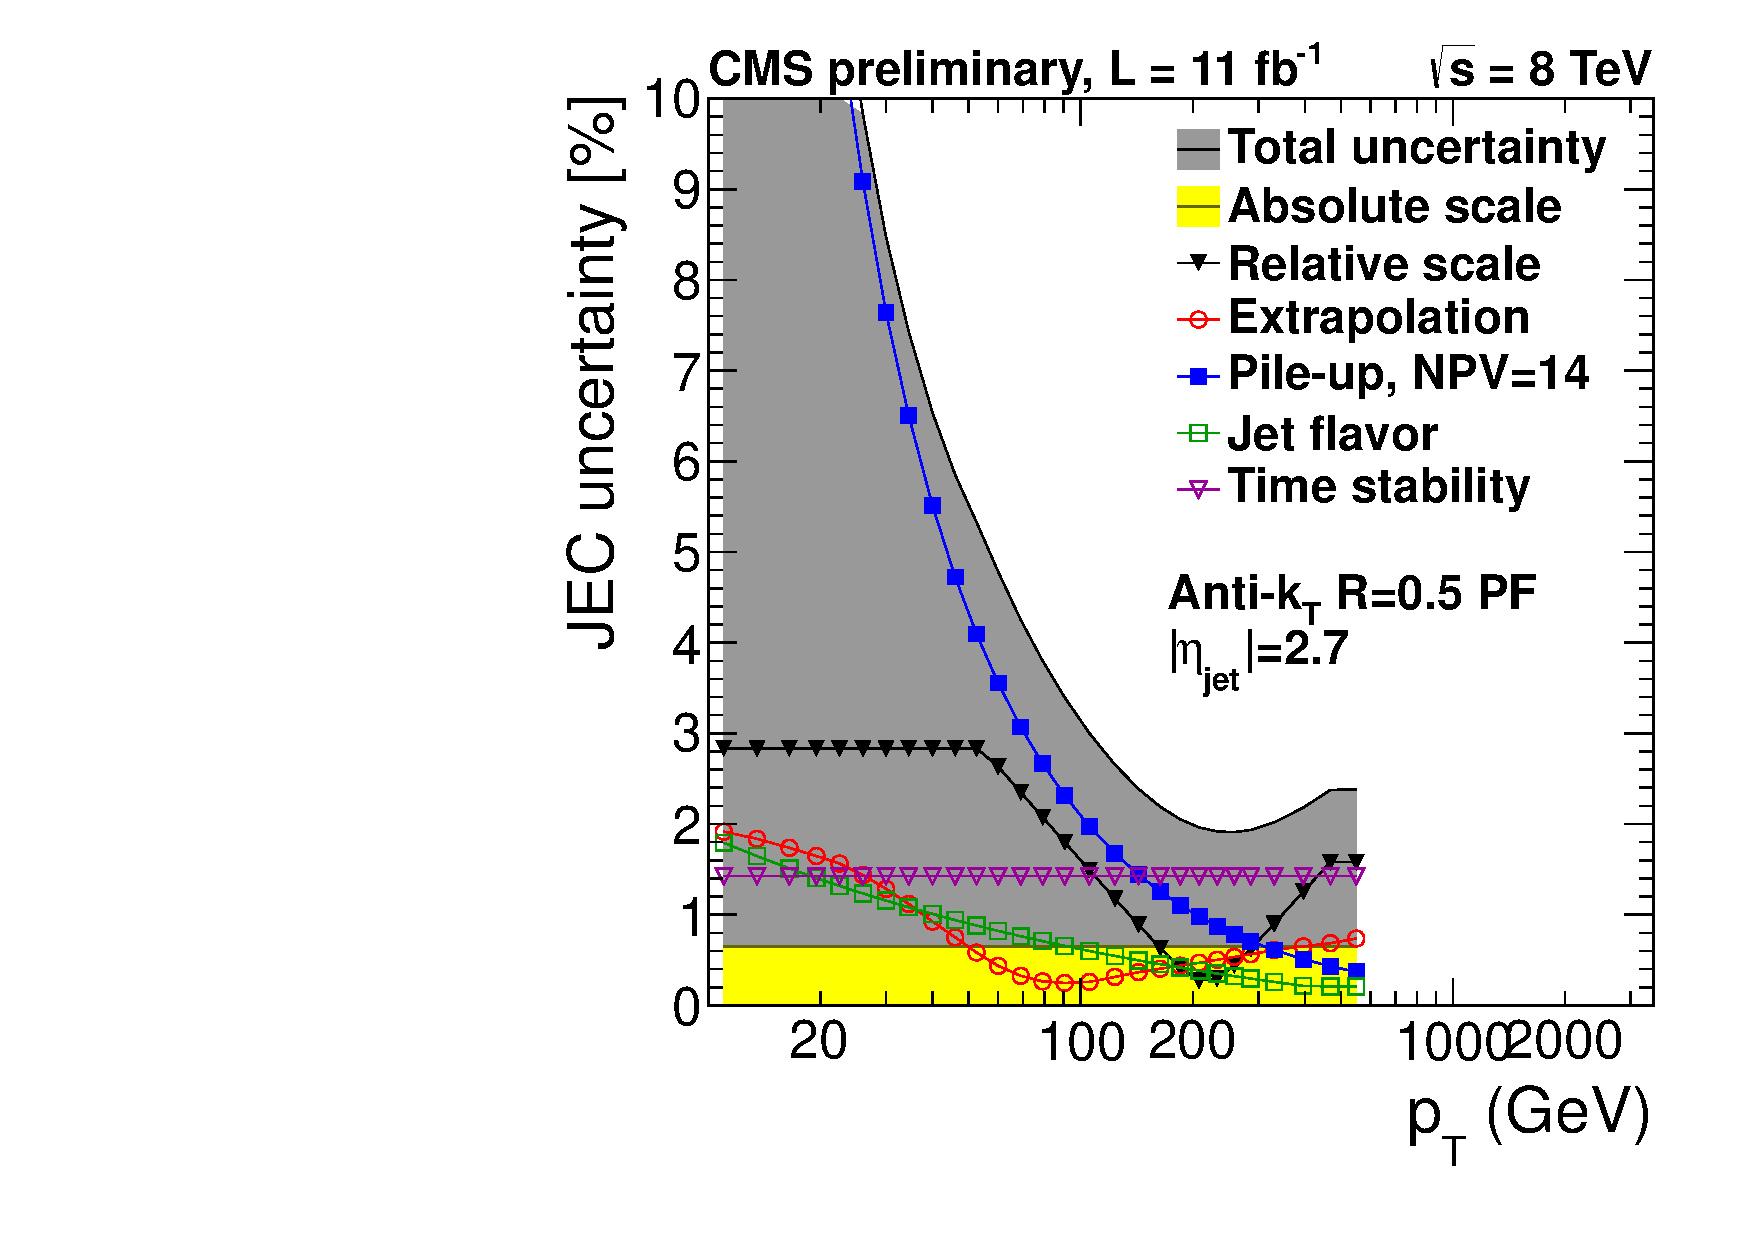
\includegraphics[width=.45\textwidth]{figures/JECUncert_Fall12_DATA_AK5PF_Eta27.pdf} 
%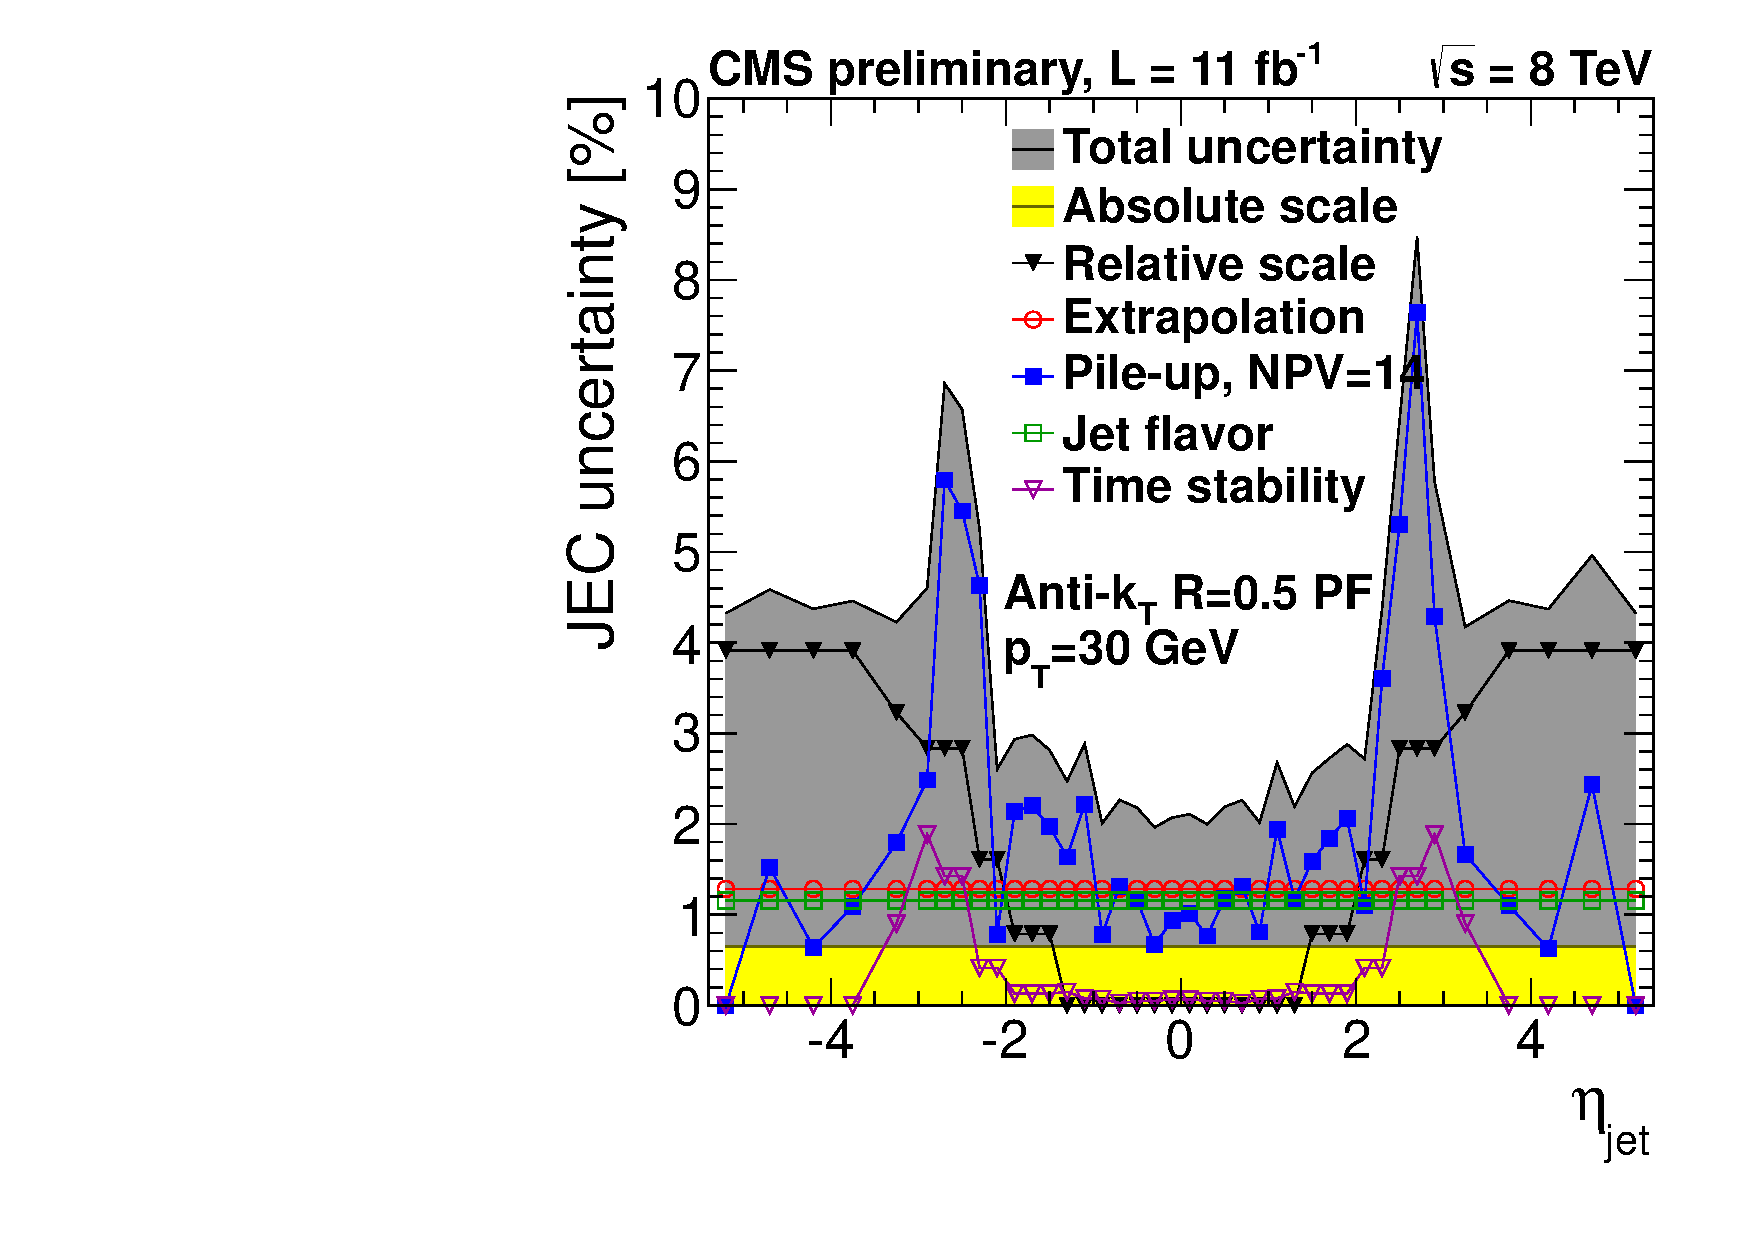
\includegraphics[width=.3\textwidth]{figures/JECUncert_Fall12_DATA_AK5PF_Pt30.pdf}
%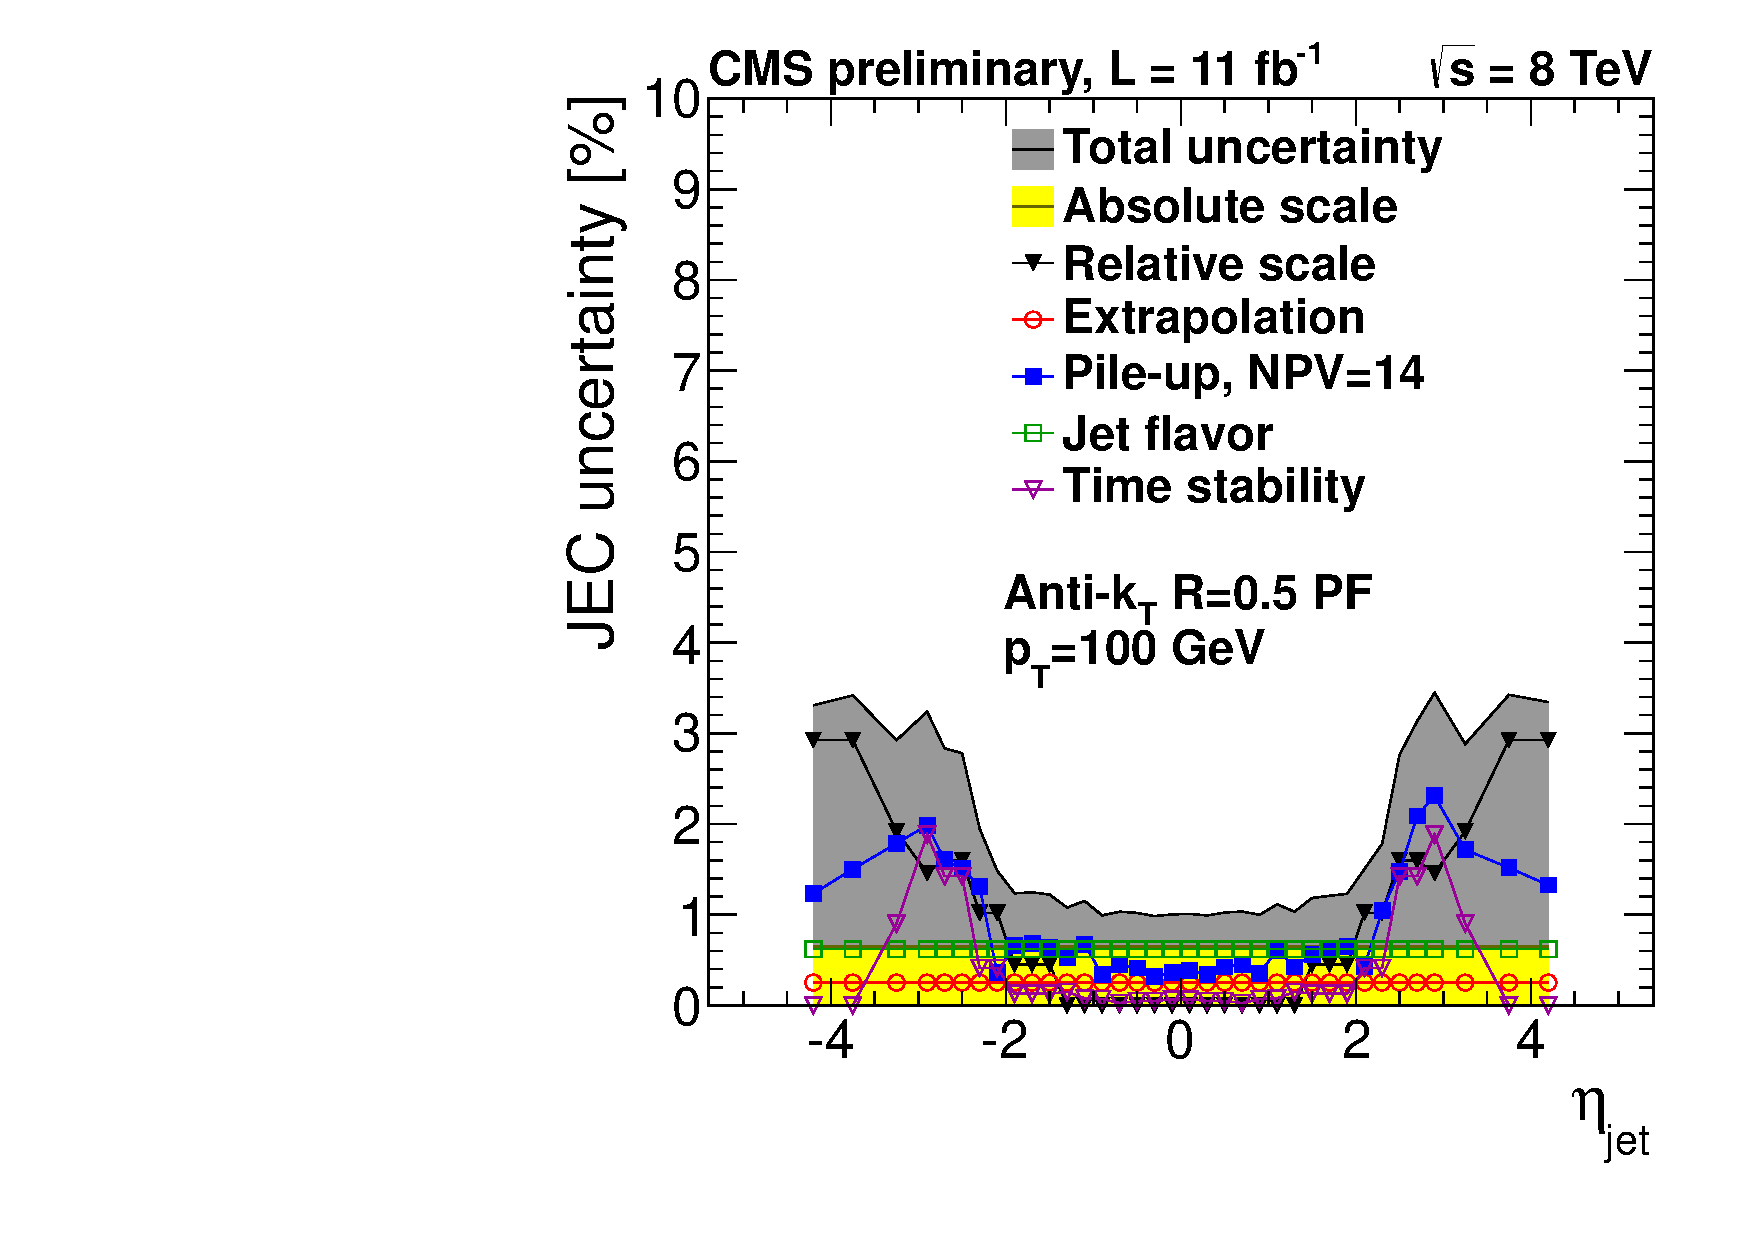
\includegraphics[width=.3\textwidth]{figures/JECUncert_Fall12_DATA_AK5PF_Pt100.pdf}
\caption{JEC uncertainty meausred in data of $\intlumi=11~\ifb$~\cite{DPS-2013-011}.}
\label{fig:jecuncert}
\end{figure}



%%%%%%%%%%%%%%%%%%%%%%%%%%%%%%%%%%%%%%%%%%%%%%%%%%%%%%%%%%%%%%%%%%
\section{ Missing Transverse Energy }

When neutrinos are produced at colliders, they do not leave any signatures
in the detector, so they can not be reconstructed. However, we can infer 
the existence of them, or any weakly-interacting particles, by computing 
the imbalance in the vector sum of transverse momenta of the reconstructed particles.
The transverse momentum of the initial particles is zero 
\footnote{It is not perfectly zero because partons have transverse movements 
inside the proton. But, the energy of their motion is at most a few hundred \MeV\
which is much less than the resolution of measurements.}.
By momentum convervation, the total momentum of the particles produced 
after collisions should be 0 as well. 
So, if the transverse momenta of all particles in the final state are summed up, 
the negative value of the vector sum should correspond to the transverse momentum 
sum of neutrinos. Thus, we define ``Missing Transverse Energy(\met)"
as the negative value of the sum of all PF candiates momenta, 
\begin{eqnarray} 
\overrightarrow{\met} = - \sum^{\textrm{All PF candidates}}_i \overrightarrow{\pt}(i).
\end{eqnarray} 

The $\phi$ distribution of true \met\ should be flat because of the rotational 
symmetry of collisions with respect to the beam axis. However, possibly due to 
the anisotropic detector response, inactive calorimeter response, detector misalignments, 
and displacement of the beam spot, the $\phi$ distributions of \met\ in both 
MC and data are not flat, but a sinusoidal shape with a period $2\pi$. 
Thus, we correct this by shifting the origin of the coordinates 
in the transverse momentum plane for x and y components individually. 
Since the size of the shift increases 
linearly as a function of number of reconstructed primary vertices, 
the form of correction is given by 
\begin{eqnarray} 
\alpha + \beta N_{\textrm{vertex}}
\end{eqnarray} 
where $\alpha$ and $\beta$ shown in Table~\ref{tab:metxycorrection} are constants 
and $N_{\textrm{vertex}}$ is the number of primary vertices. 
\begin{table}[htp] 
\begin{center} 
\begin{tabular}{c||c|c|c} 
\hline 
                       &                  & $\alpha$ &  $\beta$  \\
\hline \hline 
\multirow{2}{*}{MC}    & correction for X & $-3.00 \times 10^{-2}$ & $-6.62\times 10^{-2}$  \\
                       & correction for Y & $3.71\times 10^{-1}$   & $-1.49\times 10^{-1}$  \\
\hline 
\multirow{2}{*}{Data}  & correction for X & $3.54\times 10^{-1}$   & $2.65\times 10^{-1}$   \\
                       & correction for Y & $1.89\times 10^{-1}$   & $1.66\times 10^{-1}$   \\
\hline 
%    metx -= (+3.54233e-01 + 2.65299e-01*nvtx_);
%    mety -= (+1.88923e-01 - 1.66425e-01*nvtx_);
%    metx -= (-2.99576e-02 - 6.61932e-02*nvtx_);
%    mety -= (+3.70819e-01 - 1.48617e-01*nvtx_);
\end{tabular} 
\caption{Parameters used for XY shift correction for \met.} 
\label{tab:metxycorrection} 
\end{center} 
\end{table} 
%\textcolor{red}{optional : show the met distribution before/after the correction}

%FIXME I am here 
The performance of \met\ reconstruction is severely degraded 
in the high luminosity environment because of the random contribution of paricles 
from pileup to the \met\ calculation. 
\begin{figure}[htp] 
\centering 
\begin{tabular}{c} 
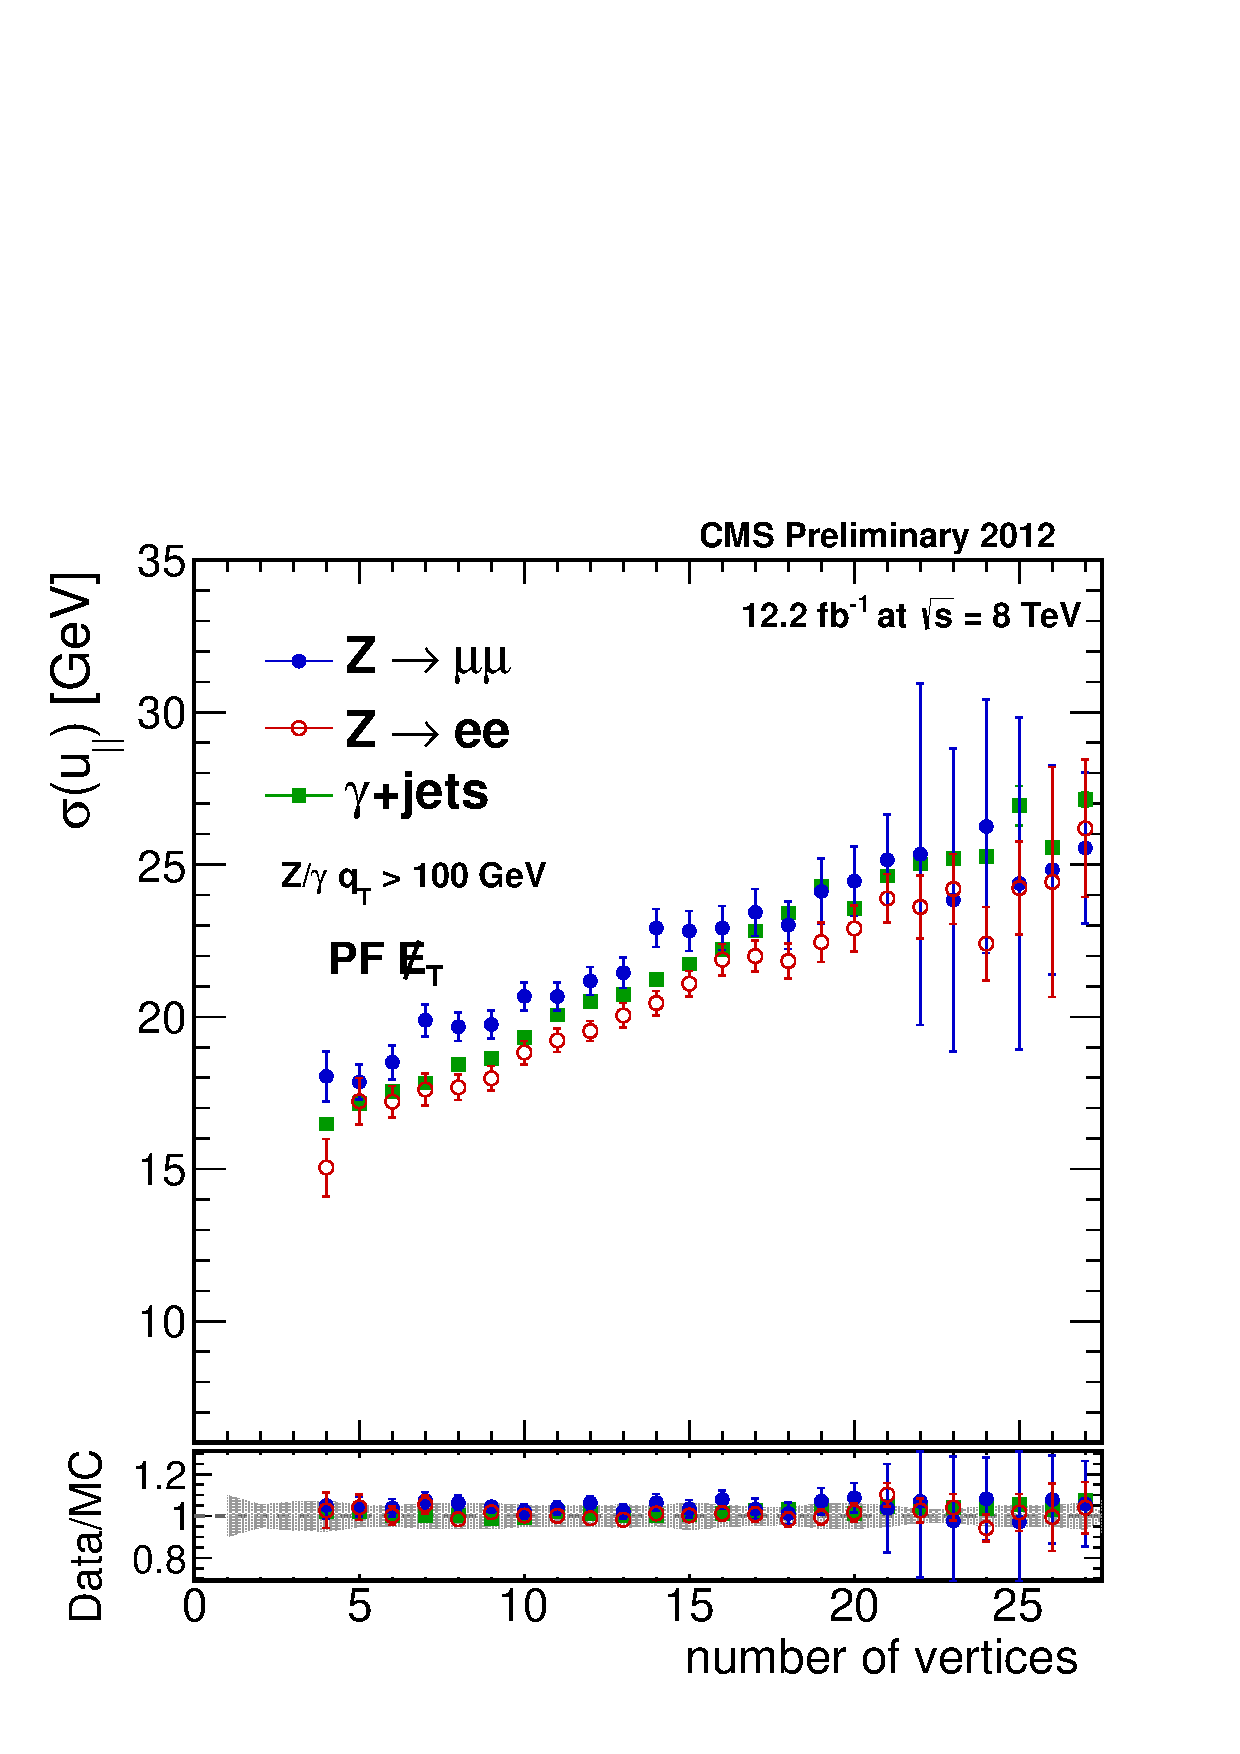
\includegraphics[width=0.45\textwidth]{figures/Fig11PFresoNVW_para_fit.pdf} 
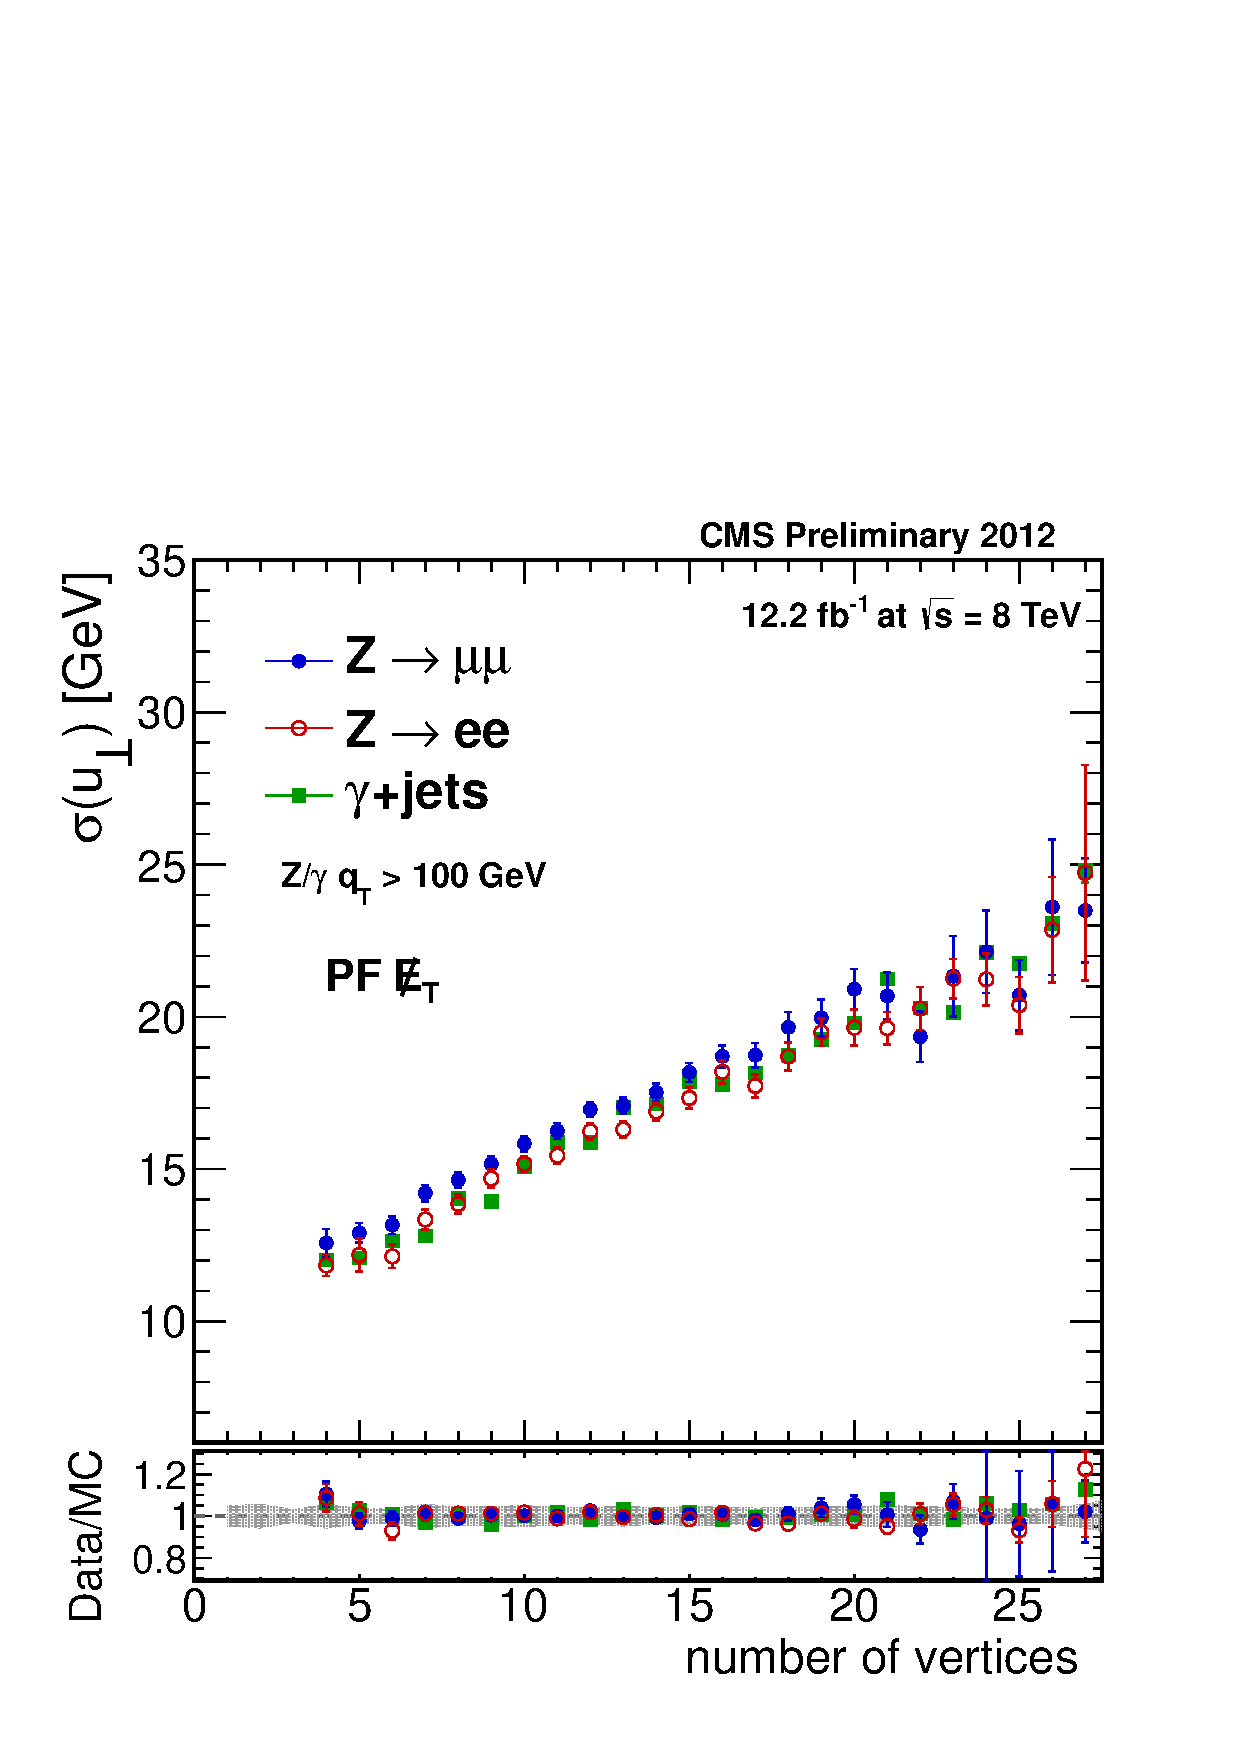
\includegraphics[width=0.45\textwidth]{figures/Fig11PFresoNVW_perp_fit.pdf} 
\end{tabular} 
\caption{The resolution of parallel(left) and perpendicular(right) components of the
hadronic recoil in the data events with Z or photon as a function of reconstructed
vertices~\cite{CMS-PAS-JME-12-002}.} 
\label{fig:metres} 
\end{figure} 
Fig.~\ref{fig:metres} shows the resolution of parallel and perpendicular components of 
the hadronic recoil in the data events with Z or photon as a function of reconstructed 
vertices~\cite{CMS-PAS-JME-12-002}. These events do not have genuine source of 
\met, \textit{i.e.} no neutrinos in the final state, so \met\ originates from 
the mis-measurement of objects. Since electons, muons 
and photons are well-measured, the dominant contribution comes from the momentum 
mis-measurement of the recoling jets. The plots clearly show that the resolution 
of the recoiling jet momentum increases as the number of vertices increases.   
So, we use another definition of \met\ which is calculated with only charged 
PF candidates associated with the event primary vertex. Because the particles from 
other vertices than the event primary vertex are excluded in the \met\ calculation,
the \met\ calculated using this method is independent of number of pileups.  
This \met\ definition is called ``\trkmet" and the exact definition is
\begin{eqnarray} 
\overrightarrow{\trkmet} 
= 
- \overrightarrow{\pt} (\ell_1)  
- \overrightarrow{\pt} (\ell_2)  
- \sum^{\textrm{All charged PF candidates}}_i \overrightarrow{\pt}(i)
\end{eqnarray} 
where $\overrightarrow{\pt} (\ell_1)$ and $\overrightarrow{\pt} (\ell_2)$
are the transverse momemta of the leptons. The charged PF candidates must 
meet the following requirements.
\begin{itemize}
\item The longitudinal impact parameter of the track matched to the PF candidate 
      with respect to the event primary vertex should be less than 0.1~cm. 
\item $\Delta R$ between the track matched to the PF candidate and the leptons 
      should be larger than 0.1 in order to avoid counting leptons twice. 
\end{itemize}

Fig.~\ref{fig:metcomp} shows the distributions of \pfmet\ and \trkmet\ 
for the Drell-Yan and the signal in simulation. The events with the number 
of reconstructed vertices($N_{vtx}$) greater than 20 and less than 5 
are drawn separately. In case of Drell-Yan process, \pfmet\ increases 
significantly as $N_{vtx}$ increases, while \trkmet\ does not depend 
on $N_{vtx}$. 
On the other hand, in case of signal process, the dependence 
of both \pfmet\ and \trkmet\ on $N_{vtx}$ is small. 
This indicates that if we use \pfmet\ as a cut variable, 
the rejection power of \dyll\ background will be weaker 
as $N_{vtx}$ increases while \trkmet\ does not show this 
dependence. However, \trkmet\ has a shortcoming that it has 
a longer tail than \pfmet\ in \dyll\ events. 
Therefore, we use both \met\ variables to suppress \dyll.

\begin{figure}[htp] 
\centering 
\begin{tabular}{c} 
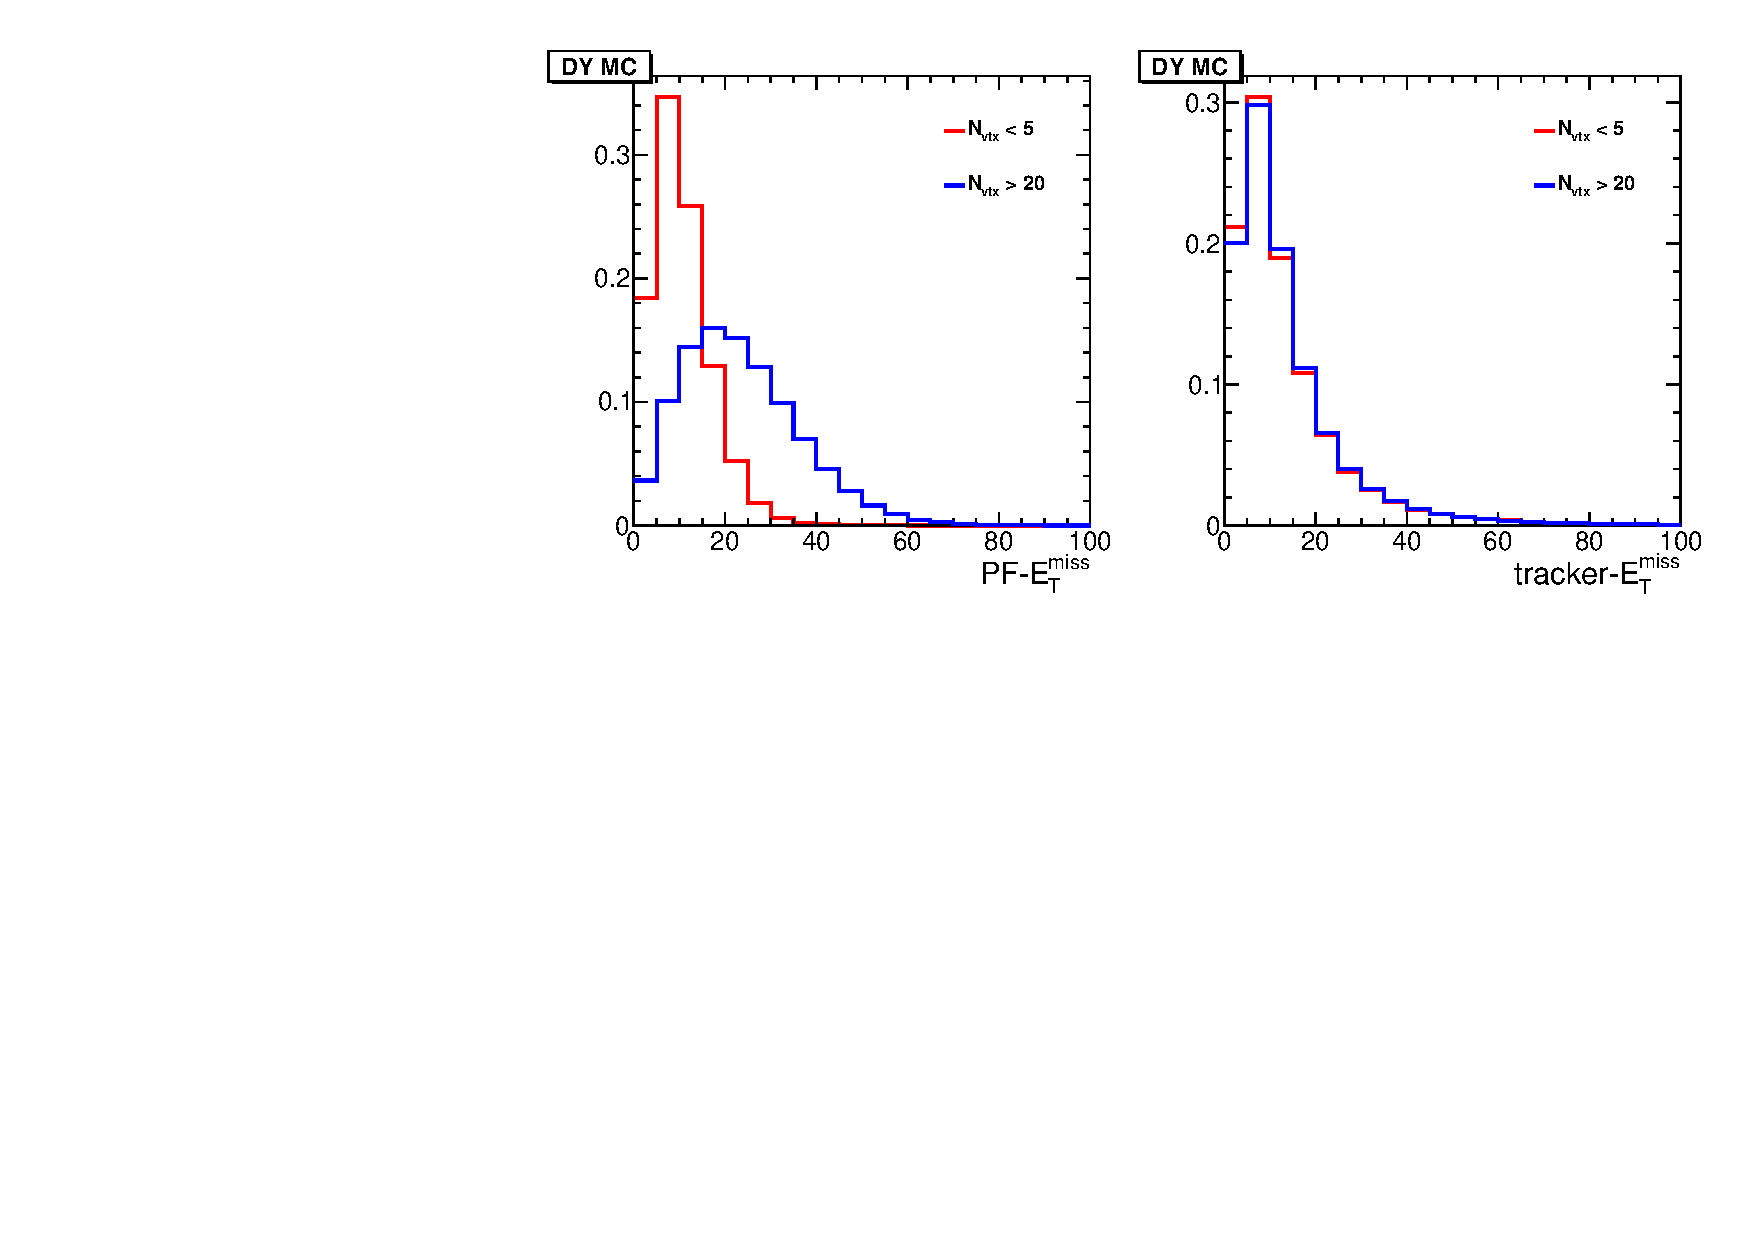
\includegraphics[width=0.9\textwidth]{figures/metcomp_dy.pdf} \\
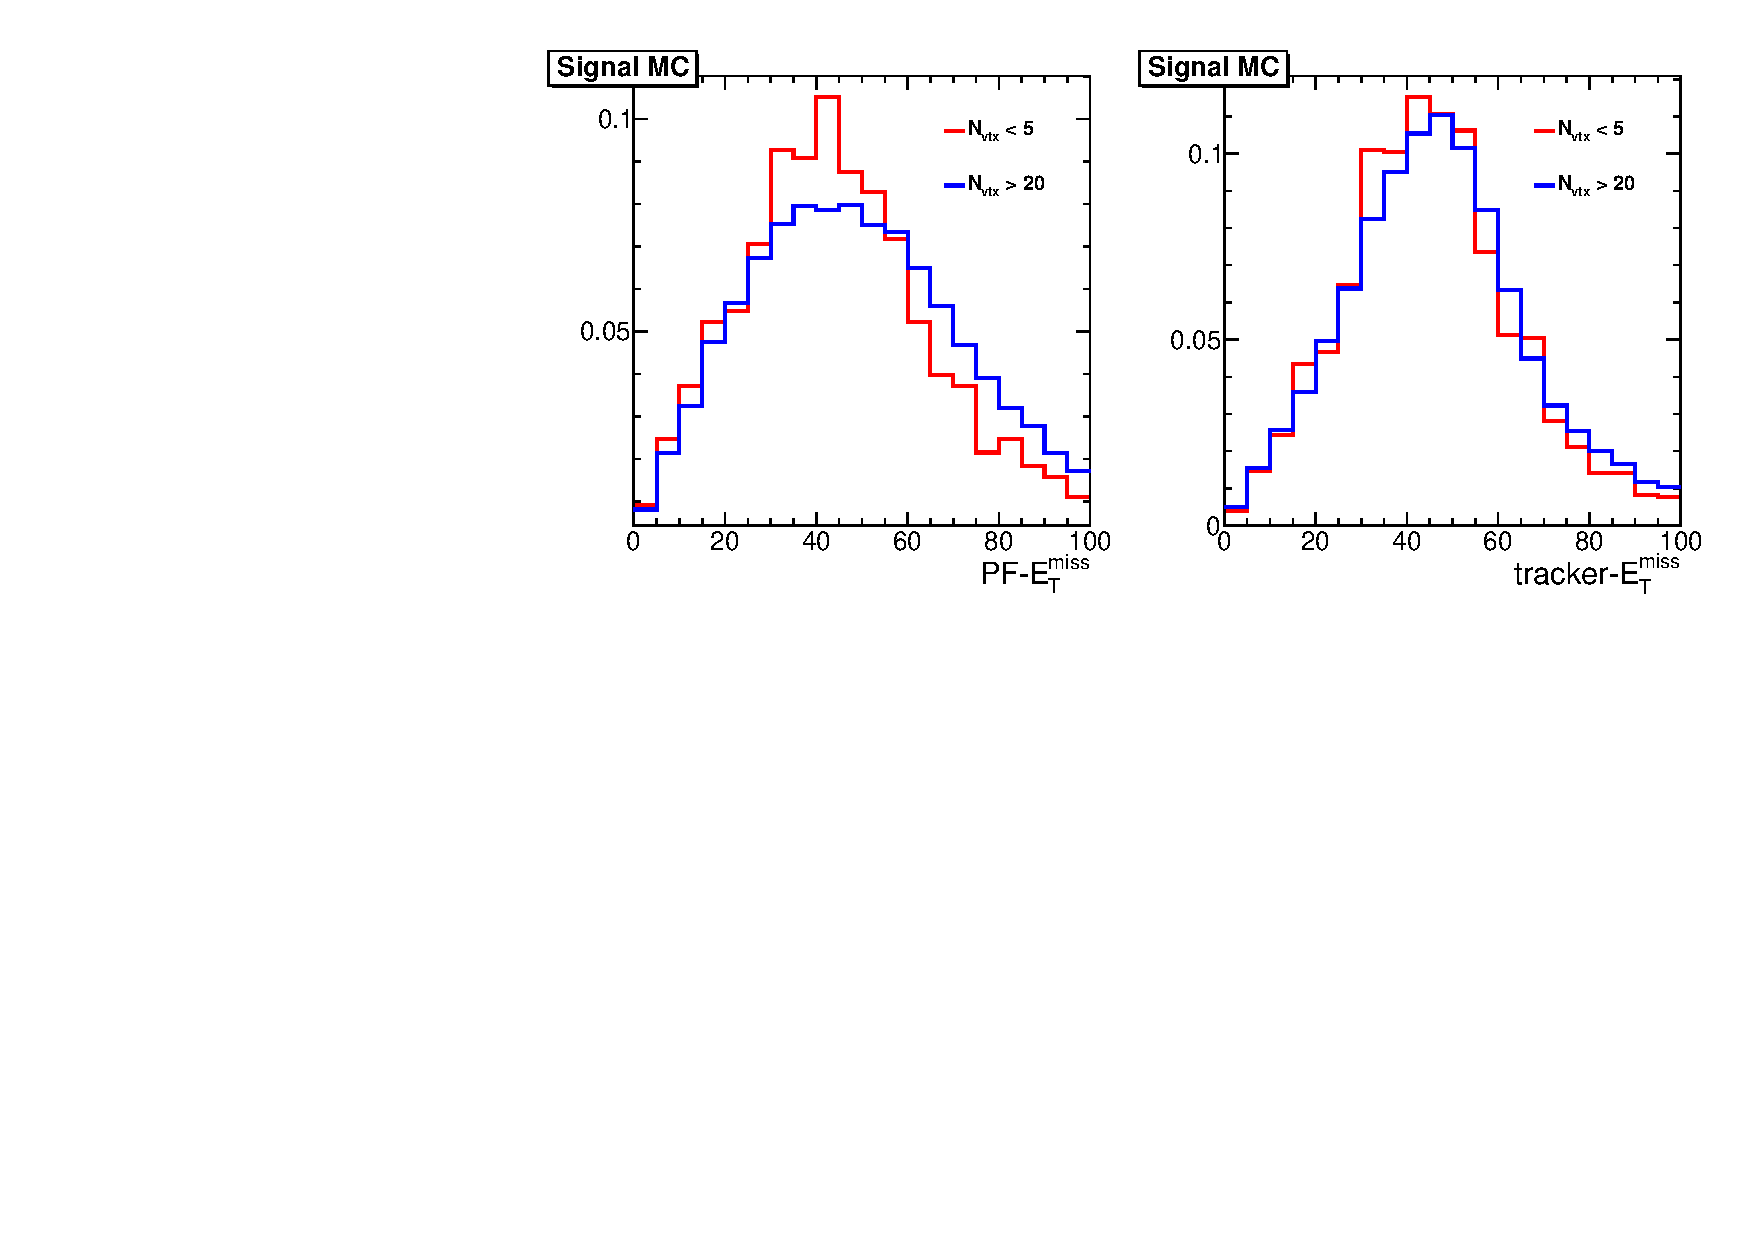
\includegraphics[width=0.9\textwidth]{figures/metcomp_sig.pdf}
\end{tabular} 
\caption{Distributions of \pfmet\ and \trkmet\
for the Drell-Yan(top) and the signal(bottom) in simulation. 
The events with the number of reconstructed vertices($N_{vtx}$) 
greater than 20(blue) and less than 5(red) are drawn separately.}
\label{fig:metcomp} 
\end{figure} 

%%%%%%%%%%%%%%%%%%%%%%%%%%%%%%%%%%%%%%%%%%%%%%%%%%%%%%%%%%%%%%%%%%
\section{ B-tagging }
\label{sec:btagging}
%\begin{itemize}
%\item \textcolor{red}{How B-tagging algorithm works and working point
%      (TCHEM : Track Counting High Efficiency Medium)}
%\item \textcolor{red}{how the discriminating variable is calculated }
%\item \textcolor{red}{quote some performance plots }
%\item \textcolor{red}{soft-muon tagging requirement }
%\end{itemize}

The presence of a bottom quark in an event is manifested by the presence 
a displaced secondary vertex. 
The bottom quark is hadronized to a B meson($\textrm{B}^0, \textrm{B}^\pm, ...$), 
and traverses over a measurable distance($c\tau \approx 500~\um$) before decaying into 
another particles. Therefore, some b-tagging algorithms use 
the distance between the primary vertex and the secondary vertex. 
In addition, using the fact that the impact parameter of the displaced 
tracks with respect to the primary vertex is larger than the one 
of the tracks from the primary vertex, some algorithms use the information 
of the impact parameter(IP). In this analysis, we use an algorithm that 
uses the IP information. 

\begin{figure}[htp] 
\centering 
\begin{tabular}{c} 
\includegraphics[width=0.99\textwidth]{figures/Btag.pdf} 
\end{tabular} 
\caption{A schematic of b-taging algorithm.}
\label{fig:btag} 
\end{figure} 
The IP is calculated in 3D thanks to the good resolution of the 
pixel detector in z direction. The IP can be signed($+$ or $-$) 
depending on the position of the associated track. 
The sign is obtained from the sign of the scalar product of 
IP vector from the primary vertex and the direction vector of the jet 
to which the track belongs as shown in Fig.~\ref{fig:btag}.
Ideally, for the decays with a sizable lifetime the IP should be large and positive, 
but it is not always positive in case the real direction of the B meson 
is different from the direction of the jet. But, they still tend to be positive. 
For the decays with very short lifetiem or random tracks, 
the IP is small and symmetric around 0.   
These are well shown in the left plot of fig~\ref{fig:btagperformance}.

The b-tagging algorithm used in this analysis is 
``TrkCountingHighEff(TCHE)~\cite{Chatrchyan:1494669}".
This algorithm uses the impact parameter significance, $S_{IP} = IP / \sigma_{IP}$ 
where $\sigma_{IP}$ is the uncertainty of the IP measurement, 
as a discribinating variable. The algorithm requires at least 2 tracks to have $S_{IP}$ 
above a given threshold. Thus, the discriminator is the $S_{IP}$ of the jet 
which has the second highest $\sigma_{IP}$. 

\begin{figure}[htp] 
\centering 
\begin{tabular}{c} 
\includegraphics[width=0.45\textwidth]{figures/TCHE.pdf}
\includegraphics[width=0.45\textwidth]{figures/Figure_007-a.pdf}
\end{tabular} 
\caption{Distribution of the discriminating variable for b-tagging is shown 
on the left. MC and data shows a good agreement.   
The b-tagging efficiency(x-axis) and mis-tag rate of udsg jets(y-axis) 
are shown on the right.}
\label{fig:btagperformance} 
\end{figure} 
Fig~\ref{fig:btagperformance} shows the distribution of the discriminator of the 
TCHE algorithm in MC and data, and 
the b-tagging efficiency(x-axis) and mis-tag rate of udsg jets(y-axis). 
The tagging efficiency of TCHE at the same mis-tag rate is not the best as 
shown on the right plot. At the working point of this analysis which is close 
to 8~\% mistag rate, b-tagging efficiency is about 10~\% lower than the 
best-performing tagger. But, this tagger was selected for this analysis 
because it is the best-performing tagger of the ones that show good agreement 
between MC and data. 


%
\chapter{Event Selection}
\label{ch:event_selection}
Using the reconstructed objects discussed in the previous chapter, 
we can select the Higgs events by selecting events with two leptons 
and \met. But, the selected events contain not only signal, 
but also backgrounds. A challege is that the production rate 
of the backgrounds is much larger than that of signal. 
\begin{figure}[htp] 
\centering 
\begin{tabular}{c} 
\includegraphics[width=0.95\textwidth]{figures/BkgProdRate.pdf} 
\end{tabular} 
\caption{The cross section $\times$
branching ratio($\sigma \times BR$) for the major background
processes and the SM \mHi=125~\GeV\ hypothesis.} 
\label{fig:bkgprodrate} 
\end{figure} 
Fig.~\ref{fig:bkgprodrate} shows the cross section $\times$ 
branching ratio($\sigma \times BR$) for the major background 
processes and the SM \mHi=125~\GeV\ hypothesis. 
The production rate of backgrounds is much larger than the signal. 
For example, the $\sigma \times BR$ of the \Wjets\ is a factor of 
$\mathcal{O}(10^5)$ larger than that of signal.  
Therefore, we need to apply stringent requirements which 
select the signal events with high efficiency, and suppress 
background events with a high rejection rate.  

The backgrounds can be divided into two categories depending on 
the way they can be suppressed. The first kind is reducible 
backgrounds which can be suppressed by tighting the requirements 
on the object selection. The other kind is irreducible backgrounds 
which have the exactly same final states as signal, 
therefore they can not be suppressed by tightening object selections,  
but by using event kinematics. 

This section describes the selection criteria to suppress the
reducible backgrounds. The requirements are imposed to 
trigger, vertex, electron, muon, jets, and top-tagging. 
In addition, there are additional requirements to suppress 
particular backgrounds. All these requirements are designed 
to select events containing a pair of Ws to make a subset of 
sample with a reasonable signal-to-background ratio for 
signal extraction. 


%%%%%%%%%%%%%%%%%%%%%%%%%%%%%%%%%%%%%%%%%%%%%%%%%%%%%%%%%%%%%%%%%%
\section{Trigger}

As seen in section~\ref{subsec:kinimetic_variables}, \hww{} events have trailing lepton 
whose transverse momentum goes down very low for low \mHi{} hypotheses. 
But, triggering low 
\pt{} leptons is very challenging because of large background events. 
Therefore, in order to record signal events with high efficiency, 
we need to trigger on the leading lepton, 
or on the both leptons. The option to trigger on the leading lepton 
is not possible because the identification 
and isolation requirements should be very tight, and momentum threshold should be very 
high to maintain a sustainable bandwidth. Thus, we trigger on the both leptons. 
The double-lepton triggers we designed for this analysis have high efficiency for  
signal events, but are loose enough to collect events in the several control regions 
we use for various studies. We also use control region triggers that allow 
fake rate and lepton selection efficiency measurements with a precision
good enough for this analysis. 

%\textcolor{red}{Where can I check the bandwidth of triggers? want to know 
%the total bandwidth of CMS and the bandwidth of triggers we use}

\subsection{Analysis Triggers}

The double-lepton triggers that are listed in Table~\ref{tab:trg_doublelepton} require 
two HLT objects, and each of them is required to match an L1 seed. The offline lepton \pt{} 
requirement is 20/10 \GeV, so the online lepton \pt{} reuquirement is a bit looser, 17/8 \GeV, 
in order to be avoid loosing events by online selection. In addition,
the longitudinal distance between the two vertices of the leptons is required 
to be less than 0.2~cm in order to suppress pileup events. 

For electron HLT objects there are additional requirements on
the shower shapes, %(H/E, $\sigma_{\eta\eta}$), 
the track-to-cluster matching and 
%($|\Delta\eta|$, $|\Delta\phi|$, $|\frac{1}{E}-\frac{1}{p}|$),
the track/calorimeter isolation. %(ECalIso, HCalIso, TrkIso). 
The exact variables and cut values are described in Table~\ref{tab:trg_requirement_def}.
In the table, the naming convention of CMS HLT triggers are shown 
with the corresponding requirements. 
The H/E is the ratio of energy deposit in HCAL to that of ECAL. 
The $\sigma_{\eta\eta}$ is the weighted sum of \Eta{} difference between the 
seed crystal and the 5x5 crystals surrouding it.   
The $|\Delta\eta|(|\Delta\phi|)$ is the difference in absolute value between 
the center of the supercluster and the direction of the track trajectory 
in \Eta($\phi$) direction.   
The $|\frac{1}{E}-\frac{1}{p}|$ is the difference between 
the reciprocal of supercluster energy 
and the reciprocal of the track momentum.  
The $\mathrm{ECalIso/E_T}$, $\mathrm{HCalIso/E_T}$ and $\mathrm{TrkIso/E_T}$ 
are the sum of the trasverse energy within $dR<0.3$ % \textcolor{red}{(checked)} 
around the center of the energy deposit or the track trajectory
divided by the transverse energy, $\mathrm{E_T}$. 
% E_T(SC) for Ecal, and elecand.pt() for Hcal and Tk (guess this is track momentum)  
Because online variables are constructed using more simplified algorithms 
than the offline variables, 
they do not exactly correspond to the offline ones. To account for this, we measure 
the trigger efficiency with respect to the offline selection, 
and apply corrections accordingly. 
The details on this can be found in~\ref{subsec:trg_eff} where the 
measurement on the trigger efficiency is discussed.
%\textcolor{red}{what is TkMu8? what is the iso requirement on single muon triggers?} 

\begin{table}[!ht]
  \centering 
  \begin{tabular} {l|l}
  \hline
  Double-lepton trigger name & L1 seed \\
  \hline \hline
  HLT\_Ele17\_CaloIdT\_CaloIsoVL\_TrkIdVL\_TrkIsoVL\_ 	    &  L1\_DoubleEG\_13\_7  \\
  Ele8\_CaloIdT\_CaloIsoVL\_TrkIdVL\_TrkIsoVL\_v[15-19] 	&                       \\ 
  %190456-190738 %190762-191419 %191512-194533
  \hline
  HLT\_Mu17\_Mu8\_v[16-22] 	    & L1\_DoubleMu\_10\_Open    \\ %190456-193686 %193806-194533
  HLT\_Mu17\_TkMu8\_v[9-14] 	& OR L1\_DoubleMu\_10\_3p5  \\ %190456-193686 %193806-194533
  \hline
  HLT\_Mu17\_Ele8\_CaloIdT\_CaloIsoVL\_ 	& L1\_Mu12\_EG7     \\
  TrkIdVL\_TrkIsoVL\_v[4-9] 	            &     \\
  %190456-190738 %190762-191419 %191512-193686 %193806-194533
  HLT\_Mu8\_Ele17\_CaloIdT\_CaloIsoVL\_	    & L1\_MuOpen\_EG12       \\ 
  TrkIdVL\_TrkIsoVL\_v[4-9] 	            & OR L1\_Mu3p5\_EG12     \\ 
  %190456-190738 %190762-191419 %191512-193686 %193806-194533
  \hline
  \end{tabular} 
  \caption{Double-lepton triggers used to collect signal events.} 
  \label{tab:trg_doublelepton}
\end{table}
%
\begin{table}[!ht]
  \centering 
  \begin{tabular} {l|l}
  \hline
  Single-lepton trigger name & L1 seed \\
  \hline \hline
  HLT\_Ele27\_WP80\_v[8-11] & L1\_SingleEG20 OR L1\_SingleEG22  \\ 
  %190456-190738 %190762-191419 %191512-194533
  \hline 
  HLT\_IsoMu24\_eta2p1\_v[11-15]   & L1\_SingleMu16er  \\  
  %190456-190738 %190762-193686 %193806-194533
  \hline \hline
  \end{tabular}
  \caption{Single-lepton triggers used to collect signal events.} 
  \label{tab:trg_singlelepton}
\end{table}

%
\begin{table}[!ht]
 \centering
 \begin{tabular}{l|c}
   \hline
   name                       &  criterion \\
   \hline \hline
   \multirow{2}{*}{CaloId\_T} & $\mathrm{H/E < 0.15 (0.10) }$ \\
                               & $\sigma_{\eta\eta}\mathrm{< 0.011\;(0.031)}$ \\
    \hline
   \multirow{2}{*}{CaloId\_VT} & $\mathrm{H/E < 0.05 (0.05) }$ \\
                               & $\sigma_{\eta\eta}\mathrm{< 0.011\;(0.031)}$  \\
    \hline \hline
    \multirow{2}{*}{TrkId\_VL} & $|\Delta\eta|\mathrm{< 0.01\; (0.01)}$ \\
                               & $|\Delta\phi|\mathrm{< 0.15\;(0.10)}$  \\
    \hline
    \multirow{2}{*}{TrkId\_T} & $|\Delta\eta|\mathrm{< 0.008\; (0.008)}$ \\
                              & $|\Delta\phi|\mathrm{< 0.07\;(0.05)}$ \\
    \hline \hline
    \multirow{2}{*}{CaloIso\_VL} & $\mathrm{ECalIso/E_T <0.2\;(0.2)}$ \\
                                 & $\mathrm{HCalIso/E_T <0.2\;(0.2)}$ \\
    \hline
    \multirow{2}{*}{CaloIso\_T} & $\mathrm{ECalIso/E_T <0.15\;(0.075)}$ \\
                                 & $\mathrm{HCalIso/E_T <0.15\;(0.075)}$ \\
    \hline
    \multirow{2}{*}{CaloIso\_VT} & $\mathrm{ECalIso/E_T <0.05\;(0.05)}$ \\
                                 & $\mathrm{HCalIso/E_T <0.05\;(0.05)}$ \\
    \hline \hline
    TrkIso\_VL                   & $\mathrm{TrkIso/E_T <0.2\;(0.2)}$ \\
    \hline
    TrkIso\_T                   & $\mathrm{TrkIso/E_T <0.15\;(0.075)}$ \\
    \hline
    TrkIso\_VT                   & $\mathrm{TrkIso/E_T <0.05\;(0.05)}$ \\
    \hline \hline
    \multirow{8}{*}{WP80} 		& $\mathrm{H/E < 0.10 (0.05) }$ \\
                               	& $\sigma_{\eta\eta}\mathrm{< 0.01\;(0.03)}$ \\
    							& $|\Delta\eta|\mathrm{< 0.007\; (0.007)}$ \\
                               	& $|\Delta\phi|\mathrm{< 0.06\;(0.03)}$  \\
                               	& $|\frac{1}{E}-\frac{1}{p}|\mathrm{< 0.05\;(0.05)}$  \\
    							& $\mathrm{ECalIso/E_T <0.15\;(0.10)}$ \\
                                & $\mathrm{HCalIso/E_T <0.10\;(0.10)}$ \\
                       			& $\mathrm{TrkIso/E_T <0.05\;(0.05)}$\\
    \hline
 \end{tabular}
 \caption{Summary of requirements applied to electrons in the analysis triggers.
The selection requirements are shown for electrons in the barrel (endcap).
The abbrevation in the names means L=Loose, VL=Very Loose, T=Tight, and VT=Very Tight.}
 \label{tab:trg_requirement_def}
\end{table}

\subsection{Utility Triggers}

The efficiency measurements of the lepton selection requirements 
are performed using the \tnp{} method~\cite{} on \dyll{} events. 
In order to use \tnp{} method, we should select a pure sample 
of \dyll{} events to reduce bias due to selecting non-prompt leptons from 
other background processes or pileup. Apart from the analysis triggers, for this 
measurement we do not have to select all available events, but a pure sample with 
an adequate statistics. The single lepton triggers used to collect signal events, 
listed in Table~\ref{tab:trg_singlelepton}, also can be used to select 
\dyll{} events. The leading lepton is likely to be triggered, making the 
trailing lepton unbiased sample that covers a wide range of 
kinematic region that streches to the low lepton \pt.   

In order to estimate jet-induced backgrounds such as \Wjets{} that have a non-prompt 
lepton that passes the full lepton selection, we use "fake rate" method.  
The details of this method are discussed in~\ref{sec:wjets}. 
In this method we define a loose lepton selection, and calculate the ratio
, fake rate, of the 
events that pass the full selection to the events that pass the loose 
selection, using a data sample of single-lepton events dominated by QCD processes. 
The fake rate differs by event kinematics
such as \pt{} and \Eta{} of the lepton, and the \pt{} of the leading jet 
that recoils off the lepton. Because the leptons in the data sample
collected by the analysis triggers are trigger objects, the loosest possible 
``loose" definition is the trigger requirement of the analysis triggers.
We devised a set of single-lepton triggers that have a loose or the same requirements 
on leptons as the double-lepton triggers. 
%Note that the single lepton triggers have tighter requirements on leptons. 
In order to cover large lepton \pt{} range, 
we use several triggers with different lepton \pt{} thresholds.
Because the jet \pt{} distribution is exponentially falling, 
we need triggers that require corrected leading jet \pt{} be greater than 30 \GeV. 
These triggers give sufficient samples for systematic study on the fake rate method. 

%For the data-driven estimation for \dyll{} backgrounds we have alternate method 
%that uses photon + jets events. These events are triggered by photon triggers 
%and the photon triggers used for this analysis are listed in the Table~\ref{tab:}.


\begin{table}[!ht]
  \begin{center}
 {\small
  \begin{tabular} {l|l}
\hline
 Trigger name & L1 seed \\
\hline\hline
 HLT\_Ele8\_CaloIdT\_TrkIdVL\_v[2-5]	& L1\_SingleEG5 		\\ %190456-190738 %190762-191419 %191512-194533
 HLT\_Ele8\_CaloIdT\_CaloIsoVL\_		& L1\_SingleEG7 		\\ 
 TrkIdVL\_TrkIsoVL\_v[12-15]			&  						\\ %190456-190738 %190762-191419 %191512-194533
 HLT\_Ele17\_CaloIdT\_CaloIsoVL\_  		& L1\_SingleEG12		\\ 
 TrkIdVL\_TrkIsoVL\_v[3-6]  			& 						\\ %190456-190738 %190762-191419 %191512-194533
 HLT\_Ele8\_CaloIdT\_CaloIsoVL\_      	& L1\_SingleEG7         \\
 TrkIdVL\_TrkIsoVL\_Jet30\_v[3-7]      	& 						\\ %190456-190738 %190762-191419 %191512-194533
 HLT\_Ele17\_CaloIdT\_CaloIsoVL\_		& L1\_SingleEG12		\\ 
 TrkIdVL\_TrkIsoVL\_Jet30\_v[3-7]		& 						\\ %190456-190738 %190762-191419 %191512-194533
	\hline \hline
 HLT\_Mu8\_v[16-18] 	&  L1\_SingleMu3  		\\ %190456 - 194533
 HLT\_Mu17\_v[3-5]      &  L1\_SingleMu12   	\\ %190456 - 194533   
%	\hline \hline
% HLT\_Photon22\_R9Id90\_HE10\_Iso40\_EBOnly\_v[2-4]					& L1\_SingleEG22		\\ %190456-190738 190762-191419 %191512-194731
% HLT\_Photon36\_R9Id90\_HE10\_Iso40\_EBOnly\_v[2-4]					& L1\_SingleEG22		\\ %190456-190738 190762-191419 %191512-194731
% HLT\_Photon50\_R9Id90\_HE10\_Iso40\_EBOnly\_v[2-4]					& L1\_SingleEG22		\\ %190456-190738 190762-191419 %191512-194731
% HLT\_Photon75\_R9Id90\_HE10\_Iso40\_EBOnly\_v[2-4]					& L1\_SingleEG22		\\ %190456-190738 190762-191419 %191512-194731
% HLT\_Photon90\_R9Id90\_HE10\_Iso40\_EBOnly\_v[2-4]					& L1\_SingleEG22		\\ %190456-190738 190762-191419 %191512-194731
    \hline 
  \end{tabular}
}
  \caption{Utility triggers for fake rate method. %and zeta method. 
  The identification and isolation requirements for electrons are described in Table~\ref{tab:trg_requirement_def}.
%The identification and isolation requirements for photons are described in Table~\ref{tab:PhotonPlusLeptonTriggerCuts}.
}
%and ``$\zeta$ method " are used for Drell-Yan background estimation.}
   \label{tab:triggers_util}
  \end{center}
\end{table}

%
%\begin{table}[htb]
%  \centering
%  \begin{tabular}{l|c}
%    \hline
%    name                        &  criterion \\
%    \hline \hline 
%    \multirow{1}{*}{R9Id90} 	& $\mathrm{R9 > 0.9 }$ \\
%    \hline 
%    \multirow{1}{*}{HE10} 		& $\mathrm{H/E < 0.1 }$ \\
%    \hline 
%    \multirow{3}{*}{Iso40}     	& $\mathrm{ECalIso} < 4.0 $ \\
%                                & $\mathrm{HCalIso} < 4.0 $ \\
%                                & $\mathrm{TrkIso}  < 4.0 $ \\
%    \hline 
%  \end{tabular}
%   \caption{Summary of requirements applied in the photon triggers used for this analysis.}
%   \label{tab:trg_requirement_def_photon}
%\end{table}

%%%%%%%%%%%%%%%%%%%%%%%%%%%%%%%%%%%%%%%%%%%%%%%%%%%%%%%%%%%%%%%%%%
\section{ Event Primary Vertex }
%\begin{itemize}
%\item \textcolor{red}{Track reconstruction : Kalman Filter, ...}
%\item \textcolor{red}{Vertex reconstruction : vertex finding, vertex fitting, ...}
%\item \textcolor{red}{Primary Vertex selection}
%\end{itemize}

The offline primary vertices are required to be within 24~\cm\ from the center of the 
detector%\textcolor{red}{(or beamspot?)} 
in z direction. 
It should be within 2~\cm\ from the beamspot in the radial direction. 
The degrees of freedom of the vertex fit should be 4 or larger. 
%\textcolor{red}{what does this mean exactly?} 

At high luminosity collisions, there are multiple proton-proton interactions 
in the same bunch crossing. In those interactions there is usually 
only one interaction that is of interest for our analysis, which triggered that event. 
These interactions tend to be associated with energetic objects, 
while the other interactions are mostly inelastic scatterings that produce soft objects.
Therefore, we choose the event primary vertex by selecting the primary vertex 
with the largest scalar sum of $\pt^2$ of tracks associated with the vertex. 
%The vertices of leptons are required to be very close to the event primary vertex.  



%%%%%%%%%%%%%%%%%%%%%%%%%%%%%%%%%%%%%%%%%%%%%%%%%%%%%%%%%%%%%%%%%%
\section{ Electron }
%\begin{itemize}
%\item \textcolor{red}{Electron reconstruction : GSF track, seeding, ... }
%\item \textcolor{red}{ID  : MVA (list of input variables, trainig samples, cut values)}
%\item \textcolor{red}{ISO : list of variables to calculate the final cut variable, cut values  }
%\end{itemize}

An electron candidate is reconstructed if there is a track and a supercluster energy 
deposit compatible with the track momentum. There are multiple sources of 
electrons which do not originate from hard interactions. These electrons 
are called ``non-prompt electrons" as opposed to the 
``prompt electrons" originated from hard interactions. 
Of these, electrons that is originated from jets is called ``fake electrons or fakes".
We can get fake electrons if  
\begin{itemize}
\item $\pi^0$ decays to two photons, and one of the two photons
      undergoes an asymmetric conversion to an electron-positron pair, \textit{i.e.}, 
      one of the them carries most of the photon momentum. 
\item $\pi^\pm$ is converted to $\pi^0$ in the ECAL(charge exchange process), 
      and the $\pi^0$ decays to a pair of photons.
\item B or D meson decays semi-leptonically.  
\end{itemize}
In order to suppress fake electrons, we apply selections composed of 
requirements on the identification,
%(track-to-supercluster matching, 
%track fit quality, shower shape, energy loss due to \brem\, ratio of hadronic energy
%to electromagnetic energy), 
isolation and impact parameter.  
Other source of non-prompt electrons is a photon conversion 
to a pair of electron and a positron 
in the material. If the conversion is asymmetric, \textit{i.e.} one particle carries 
most of the photon momentum, that particle can be selected as an electron 
candidate. Thus, we apply additional requirement on the convertion rejection.

% indentification 
For the electron identification we use a BDT-based multivariate 
approach~\cite{Chatrchyan:2012ufa}. The Boosted Decision Tree(BDT)~\cite{Hocker:2007ht} 
is a multivariate algorithm that uses distributions of multiple variables 
and their correlations to optimally distinguish one hypothesis from the other.  
The trainig is done with 2011 data; \dyll{} events for signal and QCD-dominated events 
collected by the fake rate triggers listed in section~\ref{sec:trigger}. 
In order to increase the separation, and to mitigate a possible bias 
due to the trigger selections, a set of preselection cuts that are as tight as the trigger 
requirements is applied as follows :  
\begin{itemize}
  \item $\pt>10~\GeV$ and $|\eta| < 2.5$
  \item $\sigma_{i\eta i\eta} < 0.01/0.03$ (barrel/endcap)
  \item $|\Delta\phi_{in}| < 0.15/0.10$ (barrel/endcap)
  \item $|\Delta\eta_{in}| < 0.007/0.009$ (barrel/endcap)
  \item $\textrm{H/E}< 0.12/0.10$ (barrel/endcap)
  \item $\displaystyle \frac{\sum_{\textrm{tracks with dR}<0.3}\Et}{\pt}<0.2$
  \item $\displaystyle \frac{\left(\sum_{\textrm{ECAL with dR}<0.3}\Et\right)-1}{\pt}<0.2$
  \item $\displaystyle \frac{\sum_{\textrm{HCAL with dR}<0.3}\Et}{\pt}<0.2$
\end{itemize}
%The additional subtraction of 1 GeV in the numerator of ECAL isolation is 
%to suppress the constant noise. 
The input variables to the MVA are the following.
\begin{itemize}
\item kinematics : $\pt$,  $\eta$
\item shower shape : $\sigma_{i\eta i\eta}$, $\phi_{i\eta i\eta}$, $\Delta \phi_{SC}$, $\Delta \eta_{SC}$, $E_{3\times3}/E_{5\times5}$(R9), $E_{1\times5}/E_{5\times5}$
\item track fit quality : $\chi^2(\textrm{GSF})/\textrm{ndof} $, $\chi^2(\textrm{CTF})/\textrm{ndof}$ 
\item $\textrm{N}_\textrm{layers}$  
\item cluter-track matching (geometry) : $\Delta \phi_{in}$, $\Delta \eta_{in}$, $\Delta \eta_{out}$
\item cluter-track matching (energy-momentum) : $E_{SC}/p$, $E_{C}/p_{out}$, $1/E_\textrm{SC} - 1/p$ 
\item fraction of energy carried away by \brem{} : $f_{brem}$ 
\item ratio of hadronic energy to EM energy  : $H/E$ 
\item impact parameter :  transverse and 3D impact parameters w.r.t. primary vertex
\item $E_{\textrm{PS}}/E_{\textrm{SC}}$
\end{itemize}
The $\sigma_{i\eta i\eta}$($\phi_{i\eta i\eta}$) is the weighted sum of \Eta($\phi$) 
difference between the seed crystal which contains the highest energy, 
and the $5\times5$ crystals surrouding it.
The $\Delta \phi_{SC}$($\Delta \eta_{SC}$) is the width of average distance 
between the seed crystal and the $5\times5$ crystals surrouding it.
The $E_{3\times3}/E_{5\times5}$(R9) and $E_{1\times5}/E_{5\times5}$ 
are the ratio of energy deposit in the $3\times3$($1\times5$) crystals to the
$5\times5$ crystals centered at the seed crystal. 
The $\chi^2(\textrm{GSF})/\textrm{ndof}$ and $\chi^2(\textrm{CTF})/\textrm{ndof}$
are the variables to measure the quality of GSF and CTF track fits, respectively. 
$\textrm{N}_\textrm{layers}$ is the number of tracker layers 
where the electron made hits. 
The $\Delta \phi_{in}$($\Delta \eta_{in}$) is the distance in \Eta($\phi$) direction 
between the supercluster position and the track trajectory extrapolated from 
the interaction pointto the supercluster. 
$\Delta \eta_{out}$ is the distance in \Eta{} direction
between the supercluster position and the track trajectory extrapolated 
from the supercluster to the interaction point.
The $E_{SC}/p$ is the supercluster energy divided by the track momentum 
at the point of closest approach (PCA) to the beam spot.
The $E_C/p_{out}$ is the electron cluster energy divided by the track momentum 
at the PCA to the electron cluster, extrapolated from the outermost track state. 
The $1/E_\textrm{SC} - 1/p$ is the difference between the reciprocals 
of the supercluster energy and the track momentum.
The $f_{brem}$ is the ratio of the difference between the momemta measured 
at the vertex and the outermost state to the momemtum measured at the 
vertex. This variable shows the fraction of momentum loss by \brem. 
The H/E is the ratio of the energy deposit in the HCAL tower behind the electromagnetic 
seed cluster to the energy of the seed cluster.
The $E_{\textrm{PS}}/E_{\textrm{SC}}$ is the ratio of the energy deposit in the preshower 
detector and the energy deposit in the supercluster. 
\begin{table}[!ht]
  \centering 
  \begin{tabular} {c||c|c|c}
  \hline
        & $0<|\eta|<0.8$ & $0.8<|\eta|<1.479$ & $1.479<|\eta|<2.5$\\
  \hline \hline
   $10~\GeV<\pt<20~\GeV$    & 0.0   & 0.1   & 0.62 \\ 
  \hline
   $\pt>20~\GeV$            & 0.94  & 0.85  & 0.92 \\ 
  \hline 
  \end{tabular}
  \caption{Cut values on BDT output for electron identification. Electrons with BDT output
  greater than the corresponding values in the table are considered as good electrons.} 
  \label{tab:electronid_bdtcut}
\end{table}
For selecting good electrons, we finally require that the BDT score be greater 
than the values depending on the kinematic region as shown in Table~\ref{tab:electronid_bdtcut}. 

% isolation 
The isolation requirements are imposed by computing isolation variable using 
PF candidates. 
In the high luminosity environment there are random contribution from pileup 
to the isolation calculation, so we need to correct for this to prevent 
a degradation of the isolation requirement. 
To reduce the contributions from the random charged PF candidates, they are 
required to be close to the event primary vertex. The contribution from 
the random neutral PF candidates is corrected by subracting the expected contribution. 
The variable is defined as a scalar sum of the \pt{} of the 
PF candidates satisfying the following requirements. 
\begin{itemize}
\item $\Delta R~<~0.4$ to the electron in the $\eta \times \phi$ plane
\item Other PF electrons and PF muons in the isolation cone are vetoed
\item Gamma PF candidates are required to be outside of the footprint 
      veto region of $\Delta R~<~0.08$ 
\item Charged hadron PF candidates are required to be outside of the footprint 
      veto regoin of $\Delta R~<~0.015$ 
\item Charged hadron PF candiates are required to be associated 
      with the event primary vertex : their closest vertex should be the 
      event primary vertex
\item Neutral components are corrected by subtracting pileup contribution which is 
      calculated by $\rho \times \textrm{A}_{\rm{eff}}$,
\end{itemize}
where $\rho$ is the event-by-event energy density~\cite{} calculated using 
\texttt{kt6PFJets} algorithm~\cite{}, 
and $\textrm{A}_{\textrm{eff}}$ is the effective area shown in Table~\ref{tab:electron_Aeff}. 
\begin{table}[!ht]
  \centering 
  \begin{tabular} {c||c|c|c|c|c|c}
  \hline
    $|\eta|$    & 0 - 1.0 & 1.0 - 1.479 & 1.479 - 2.0 & 2.0 - 2.2 & 2.2 - 2.3 & 2.3 - 2.4  \\
  \hline \hline
    $\textrm{A}_{\rm{eff}}$  & 0.19 & 0.25 & 0.12 & 0.21 & 0.27 & 0.44 \\ 
  \hline 
  \end{tabular}
  \caption{Effective area used for electron isolation calculation.}
  \label{tab:electron_Aeff}
\end{table}

The isolation variable we cut on is calculated as 
\begin{equation}
\frac{\rm{Iso}_{PF}}{\pt}
=
\left[ \rm{Iso}_{charged \, hadron} + \left\{ \rm{Iso}_{gamma} 
       + \rm{Iso}_{neutral \, hadron} -\rho \times \textrm{A}_{\textrm{eff}} \right\} \right]
\times \frac{1}{\pt}
\end{equation}
where $\rm{Iso}_{charged \, hadron}$, $\rm{Iso}_{gamma}$, and $\rm{Iso}_{neutral \, hadron}$ 
are the scalar sum of the \pt{} of the charged hadron, gamma and neutral hadron PF candidates, 
respectivlely, in the isolation cone of $0.4$ around the electron.
We require $\frac{\rm{Iso}_{PF}}{\pt}$ to be less than $0.15$ in both barrel and endcap.  

% conversion
In order to reject the electrons from a conversion from a photon, we reject the electron 
if there is a recontructed conversion vertex where one of the two tracks match with 
the electron, if the probability of the conversion vertex fit is greater than $10^{-6}$, 
if the distance between the conversion vertex and the point of closest approach 
to the event primary vertex is greater than 2~\cm,
and there is any missing hit in the electron track before the conversion vertex.   

% impact parameters
The impact parameter requirements are such that the transverse(longitudinal) impact parameter
between the electron track and the event primary vertex is less than 0.02 cm(0.1 cm). 

The efficiency of the full electron selection measured with 20/10~\GeV\ requirement 
in MC is about 80~\% for electrons in the \mHi=125~\GeV\ events 
and about 5~\% for electrons whose mothers are not Ws in W+jets.

%%%%%%%%%%%%%%%%%%%%%%%%%%%%%%%%%%%%%%%%%%%%%%%%%%%%%%%%%%%%%%%%%%
\section{ Muon }
%\begin{itemize}
%\item \textcolor{red}{Muon reconstruction : ...}
%\item \textcolor{red}{ID  : list variables and cut values }
%\item \textcolor{red}{ISO : MVA (list of input variables, trainig samples, cut values) }
%\end{itemize}

A muon candidate is reconstructed if there 
is a track in the tracker and/or are segments in the muon system. 
There are multiple sources of muons which do not originate from gauge boson decays. 
\begin{itemize}
\item decay-in-flight : a charged meson decays to muon in the tracker, 
\item punch-through : a charged meson survive the HCAL, and leaves 
\item B or D meson decays semi-leptonically.  
\end{itemize}
In order to reject muons from these sources, 
we apply a muon selection which is composed of requirements 
on the identification,
%(track fit quality, momentum resolution, 
%number of hits/segments in the tracker/muon system,  
%rejection of ), 
isolation and impact parameter.  

%identification
The identification requirements are as follows. 
\begin{itemize}
\item The muon should be identified as PF muon 
\item $\pt>10~\GeV$ and $|\eta|<2.4$ 
\item $N_{\textrm{track layers}}>5$ 
\item $N_{\textrm{pixel hits}}$
\item $\displaystyle \frac{\delta \pt}{\pt} < 0.1$  
\item $\displaystyle \frac{\chi^2_{\textrm{kink finder}}}{\textrm{ndof}} < 20$
\item The muon should be global muon or tracker muons  
\end{itemize}
where $N_{\textrm{layers}}$ is the number of tracker layers where the muon track made hits, 
the $N_{\textrm{pixel hits}}$ is the number of pixel hits of the muon track,
the $\displaystyle \frac{\delta \pt}{\pt}$ is the relative resolution 
of the muon \pt, 
and $\displaystyle \chi^2_{\textrm{kink finder}}/\textrm{ndof}$ is the quality 
of kink finder algorithm which finds muons from decay-in-flights.  
In addtion to these requirements, the muons are required to be the global muons with 
$\chi^2/\textrm{ndof}$ of the the global fit less than 10, 
at least one muon hit matching the global fit 
%\textcolor{red}{(what is the difference between hits and segments?)},  
and having at least two muon segments in different muon stations. 
If the moun is not a global muon, it can be a tracker muon satisfying that at least two muon 
segments one of which is in the outermost muon station are matched.  

%isolation 
For the isolation requirement, the MVA-based isolation variable~\cite{MuonRingIso} is used.
%to reduce contamination from non-isolated muons originating from jets. 
It uses the energy deposits of PF candidates of three categories, 
charged hadron, gamma and neutral hadrons in the concentric isolation cones
of size $\Delta R = 0-0.1,~0.1-0.2,~0.2-0.3,~0.3-0.4$ and $0.4-0.5$.
Neutral components are corrected by subtracting the pileup contribution which is 
calculated by $\rho \times \textrm{A}_{\textrm{eff}}$ where $\rho$ (\texttt{kt6PFJets}) is the 
event-by-event energy density and $\textrm{A}_{\textrm{eff}}$ is the effective area.  
Effective areas are from Fall 11 simulation (\texttt{kMuEAFall11MC}), and 
values are shown in Table~\ref{tab:muAeff}.  
Exact definition of input variables to the MVA is the following :
\begin{itemize}
\item PF charged hadron
	\begin{itemize}
    \item minimum of $\textrm{Iso}_\textrm{PF charged, 01}/\pt$ and 2.5	
    \item minimum of $\textrm{Iso}_\textrm{PF charged, 12}/\pt$ and 2.5	
    \item minimum of $\textrm{Iso}_\textrm{PF charged, 23}/\pt$ and 2.5	
    \item minimum of $\textrm{Iso}_\textrm{PF charged, 34}/\pt$ and 2.5	
    \item minimum of $\textrm{Iso}_\textrm{PF charged, 45}/\pt$ and 2.5	
	\end{itemize}
\item PF gamma : If negative, 0.0 is assigned
	\begin{itemize}
    \item minimum of $\left[\textrm{Iso}_\textrm{PF gamma, 01} - \rho \times \textrm{A}_{\textrm{eff}}\right]/\pt$ and 2.5 
    \item minimum of $\left[\textrm{Iso}_\textrm{PF gamma, 12} - \rho \times \textrm{A}_{\textrm{eff}}\right]/\pt$ and 2.5 
    \item minimum of $\left[\textrm{Iso}_\textrm{PF gamma, 23} - \rho \times \textrm{A}_{\textrm{eff}}\right]/\pt$ and 2.5 
    \item minimum of $\left[\textrm{Iso}_\textrm{PF gamma, 34} - \rho \times \textrm{A}_{\textrm{eff}}\right]/\pt$ and 2.5 
    \item minimum of $\left[\textrm{Iso}_\textrm{PF gamma, 45} - \rho \times \textrm{A}_{\textrm{eff}}\right]/\pt$ and 2.5 
	\end{itemize}
\item PF neutral hadron : If negative, 0.0 is assigned
	\begin{itemize}
    \item minimum of $\left[\textrm{Iso}_\textrm{PF neutral, 01} - \rho \times \textrm{A}_{\textrm{eff}}\right]/\pt$ and 2.5 
    \item minimum of $\left[\textrm{Iso}_\textrm{PF neutral, 12} - \rho \times \textrm{A}_{\textrm{eff}}\right]/\pt$ and 2.5 
    \item minimum of $\left[\textrm{Iso}_\textrm{PF neutral, 23} - \rho \times \textrm{A}_{\textrm{eff}}\right]/\pt$ and 2.5 
    \item minimum of $\left[\textrm{Iso}_\textrm{PF neutral, 34} - \rho \times \textrm{A}_{\textrm{eff}}\right]/\pt$ and 2.5 
    \item minimum of $\left[\textrm{Iso}_\textrm{PF neutral, 45} - \rho \times \textrm{A}_{\textrm{eff}}\right]/\pt$ and 2.5 
	\end{itemize}
\end{itemize}
where we define 
\begin{eqnarray} 
\textrm{Iso}_\textrm{PF,XY} 
= 
\sum_{
\begin{subarray}{l}
\textrm{PF candidates in the cone of} \\
\textrm{0.X}   < \Delta R^{\mu-\textrm{PF candidate}} < \textrm{0.Y} 
    \end{subarray} }
\pt
%\textrm{the scalar sum of \pt\ of PF candidates in the cone of 0.X} 
%< \Delta R^{\mu-\textrm{PF candidate}} < \textrm{0.Y}.
\end{eqnarray} 

We require that the MVA output be greater than 0.82 (0.86) in $10<\pt~<20~\GeV$ 
and 0.86 (0.82) in $\pt~>20~\GeV$. The cut values correspond to the ones in barrel (endcap).

\begin{table}[htp]
	\centering
		\begin{tabular}{c|c|c|c|c|c|c}
			\hline 
				\multicolumn{7}{c}{PF gamma} \\
	  	    \hline
			 	$|\eta|$     & $0.0 - 1.0$ & $1.0 - 1.479$ & $1.479 - 2.0$ & $2.0 - 2.2$ & $2.2 - 2.3$ & $2.3-$ \\       		
	  	    \hline \hline
				$0.0<dR<0.1$ & 0.004& 0.002& 0.003& 0.009& 0.003& 0.011 \\
				$0.1<dR<0.2$ & 0.012& 0.008& 0.006& 0.012& 0.019& 0.024 \\
				$0.2<dR<0.3$ & 0.026& 0.020& 0.012& 0.022& 0.027& 0.034 \\
				$0.3<dR<0.4$ & 0.042& 0.033& 0.022& 0.036& 0.059& 0.068 \\
				$0.4<dR<0.5$ & 0.060& 0.043& 0.036& 0.055& 0.092& 0.115 \\
	  	    \hline \hline 
				\multicolumn{7}{c}{PF neutral hadron} \\
	  	    \hline 
			 	$|\eta|$     & $0.0 - 1.0$ & $1.0 - 1.479$ & $1.479 - 2.0$ & $2.0 - 2.2$ & $2.2 - 2.3$ & $2.3-$ \\       		
	  	    \hline \hline
				$0.0<dR<0.1$ & 0.002& 0.004& 0.004& 0.004& 0.010& 0.014 \\
			    $0.1<dR<0.2$ & 0.005& 0.007& 0.009& 0.009& 0.015& 0.017 \\
			    $0.2<dR<0.3$ & 0.009& 0.015& 0.016& 0.018& 0.022& 0.026 \\ 
				$0.3<dR<0.4$ & 0.013& 0.021& 0.026& 0.032& 0.037& 0.042 \\ 
				$0.4<dR<0.5$ & 0.017& 0.026& 0.035& 0.046& 0.063& 0.135 \\ 
			\hline
		\end{tabular}
		\caption{ Effective areas used for muon isolation. They were calculated with Fall11 MC sample.}
	\label{tab:muAeff}
\end{table}

%impact parameter 
In addtion, we require transverse/longditudinal impact parameters 
to be associated with the event primary vertex. 
The transverse impact parameter is required 
to be less than 0.01 cm for $\pt<20~\GeV$ and 0.02 cm for $\pt>20~\GeV$. 
The longitudinal impact parameter is required to be less than 0.01 cm. 

The efficiency of the full muon selection measured with 20/10~\GeV\ requirement 
in MC is about 90~\% for muons in the \mHi=125~\GeV\ events 
and about 11~\% for muons whose mothers are not Ws in W+jets.

%%%%%%%%%%%%%%%%%%%%%%%%%%%%%%%%%%%%%%%%%%%%%%%%%%%%%%%%%%%%%%%%%%
\section{ Jet }
\label{sec:jetselection}
%\begin{itemize}
%\item \textcolor{red}{Jet reconstruction : anti-kT (dR = 0.5) }
%\item \textcolor{red}{Jet energy correction : L1Fastjet/L2/L3 (+ Residual correction in data) }
%\item \textcolor{red}{lepton veto ($dR>0.3$) }
%\item \textcolor{red}{MVA jet ID(list of input variables, training samples, cut values)}
%\item \textcolor{red}{two definitions : (1) jet bin counting($\pt>30~\GeV$) (2) top veto($10<\pt<30~\GeV$) }
% have a plot like this for MVA Jet ID? not sure how I drew this though
% maybe a script is somewhere on uaf
%http://uaf-2.t2.ucsd.edu/~jaehyeok/HWW/PhilJetIDMVA/dev/PhilJetIDMVAefssssssss.pdf
%\end{itemize}

In this analysis jets are selected by rejecting overlaps with selected electrons 
and muons. If the $\Delta R$ between a lepton and the jet is less than 0.3, the jet 
is likely to be a lepton, thus it is not considered as a jet. In the high pileup environment, 
clustering random PF particles from pileup interactions can lead to high \pt\ jets. 
To suppress this, we apply a BDT-based techique to suppress jets originated from pileups. 
The jets from pileup tend to be soft, so they need to be overlaid to pass the jet \pt\ threshold. 
Therefore, the energy deposit of the pileup jets are more spread 
than the ones from hard interactions. The following variables are used 
in the BDT-based suppression technique.
\begin{itemize}
\item Number of reconstructed primary vertices in the event
\item Kinematics of the jet : \pt, \Eta\ and $\phi$ 
\item Impact parameters of the most energetic charged PF candidates in the jet : $d_0$ and $d_Z$
\item Fraction of charged PF candidates associated with the event primary vertex(PV) 
    \begin{itemize}
    \item $\beta$   : sum \pt\ of PF candidates with $d_Z(PV) < 0.2$ 
                      divided by sum \pt\ of all PF candidates
    \item $\beta^*$ : sum \pt\ of PF candidates with $d_Z(\textrm{all vertices not PV}) < 0.2$
                      divided by sum \pt\ of all PF candidates
    \end{itemize}
\item Number of neutral and charged PF candidates in the jet
\item \pt-weighted mean of $\Delta R$ of all PF candidates in the jet 
\item Fraction of sum \pt\ of all PF candidate in the rings of $\Delta R$ = 0.0 - 0.1, 0.1 - 0.2, 0.2 - 0.3, 
      0.3 - 0.4 and 0.4 - 0.5.
\end{itemize}

We select jets of which BDT scores are greater than the values 
in Table~\ref{tab:jetidcut} which correspond to the loose working point. 
\begin{table}[htp]
\small
	\centering
		\begin{tabular}{c|c|c|c|c}
			\hline
			\pt(\GeV)	&  $0<|\eta|<2.5$ 	& $2.5<|\eta|<2.75$		& $2.75<|\eta|<3.0$ 	& $3.0<|\eta|<4.7$ 		\\ 
			\hline \hline
				 - 10 		& 0.0 				& 0.0					& 0.0	 				& 0.2					\\ 
				10 - 20 	& -0.4 				& -0.4					& -0.4	 				& 0.4					\\
				20 - 30	& 0.0 				& 0.0					& 0.2	 				& 0.6					\\ 
				30 - 		& 0.0 				& 0.0					& 0.6	 				& 0.2					\\
			\hline 
		\end{tabular}
		\caption{Cut values on jet identification MVA outputs. MVA output is required to be greater than 
				these values to be counted as a jet.}
	\label{tab:jetidcut}
\end{table}
Of the selected jets, the high \pt\ jets($\pt>30~\GeV$ and $|\Eta|<4.7$) are used for counting 
the number of jets, and the low \pt\ jets($10<\pt<30~\GeV]$ and $|\Eta|<4.7$) are used 
for rejecting top events. 
%\textcolor{red}{Any plots to show? MVA values for real jet and PU jets? or JEC factorization? 
%look at the slides I made for jet MVA id, there's veto efficiency as a function of Nvtx.} 


%%%%%%%%%%%%%%%%%%%%%%%%%%%%%%%%%%%%%%%%%%%%%%%%%%%%%%%%%%%%%%%%%%
\section{ Missing Transverse Energy }
%\begin{itemize}
%\item \textcolor{red}{define projected MET (compare signal and bkgd, (ex) \ztt)}
%\item \textcolor{red}{cut values ($\textrm{minMET} > 20~\GeV$) }
%\end{itemize}

The \met{} is used to reject processes which do not have true source of missing energy. 
Target processes are QCD and \dyll{} where \met{} is caused by  
mis-measurement of jet momentum and pileup. However, in case of \dytt{}, the \Tau{} can 
decay into lepton and neutrinos, giving true missing momentum. Because of large 
mass difference between Z and \Tau{}, \Tau{} is generally boosted significantly 
with its decay products flying in the same direction of the \Tau momentum. 
Therefore, the missing energy component perpendicular to the lepton momentum 
is a better measure for true \met{} which is originated from \Tau{} decays. 
To realize this we define ``projected \met " (\pmet) as 
\begin{equation}
\pmet 
= 
\begin{cases} \met & \text{if $\Delta\phi_{min}>\frac{\pi}{2}$,}
\\
\met\sin(\Delta\phi_{min}) & \text{if $\Delta\phi_{min}<\frac{\pi}{2}$}
\end{cases}
\end{equation}
where  
\begin{equation}
\Delta\phi_{min} =  min(\Delta\phi(\ell_1,\met),\Delta\phi(\ell_2,\met)).
\end{equation}
The $\Delta\phi(\ell_i,\met)$ is the angle between \met{} and the lepton $i$ 
on the transverse plane. Figure~\ref{fig:projmetscheme} shows the schematic 
of \pmet. 
\begin{figure}[htp] 
\centering 
\begin{tabular}{c} 
\includegraphics[width=0.7\textwidth]{figures/projmet.pdf} 
\end{tabular} 
\caption{Schematic of \pmet.}
\label{fig:projmetscheme} 
\end{figure}  
%
\begin{figure}[htp] 
\centering 
\begin{tabular}{c} 
\includegraphics[width=0.45\textwidth]{figures/pmet_met_ztt.pdf} 
\includegraphics[width=0.45\textwidth]{figures/pmet_met_hww125.pdf} 
\end{tabular} 
\caption{\met(black) and \pmet(blue) in \dytt{}(left) and SM Higgs at \mHi=125~\GeV(right).}
\label{fig:projmet} 
\end{figure}  
Figure~\ref{fig:projmet} shows the \met{} and the \pmet{} distributions 
in black and red, repectively, in \dytt{} and SM Higgs at \mHi=125~\GeV\
on left and right, repectively. We can see that \pmet is more squeezed to 
the lower values in case of \dytt, giving better rejection power.  

The \trkmet\ is a variable insensitive to the pileup, 
but a drawback is that its tail is longer than \pfmet\ in the \dyll{} events. 
By isospin symmetry the average number of neutral hadrons should 
be same as that of the charged hadrons. But, if there is an imbalance between neutral 
and charged components in the jets, the \trkmet\ can be calculated arbitrarily high. 
For example, for a di-jet event with back-to-back 30~\GeV\ jets where one jet is composed 
of 10~\GeV\ of charged components and 20~\GeV\ of neutral components, and the other jet 
has the opposite composition, the \pfmet\ is 0 while \trkmet\ is 10~\GeV. 
Therefore, we use the minimum of \pfmet\ and \trkmet\, 
\begin{eqnarray} 
\minpmet = min \left( \pmet, \ptrkmet \right), 
\end{eqnarray} 
as a \met\ variable to protect \trkmet\ from those fluctuations. 
The other advantage of taking the minimum is that the the correlation 
between the two \met\ definitions is strong in the events with true \met, 
while weak in the events with fake \met\ as shown in Fig.~\ref{fig:2dmet}. 
So, by taking the minimum of them, we can get additional rejection 
of \dyll\ backgrounds without a harm to the signal.  
%
\begin{figure}[htp] 
\centering 
\begin{tabular}{c} 
\includegraphics[width=0.99\textwidth]{figures/2dmet.pdf} 
\end{tabular} 
\caption{\pmet{} vs. \ptrkmet{} in \dyll{} and SM Higgs \mHi = 125~\GeV.}
\label{fig:2dmet} 
\end{figure}  

We require \minpmet{} to be greater than 20~\GeV\ in all categories as a baseline selecion. 
For further rejection of \dyll{} background, we apply MVA-based technique which will be 
discussed in detail in section~\ref{sec:dybkg}. 

%%%%%%%%%%%%%%%%%%%%%%%%%%%%%%%%%%%%%%%%%%%%%%%%%%%%%%%%%%%%%%%%%%
\section{ Top-tagging }
%\begin{itemize}
%\item \textcolor{red}{How B-tagging algorithm works and working point
%      (TCHEM : Track Counting High Efficiency Medium)}
%\item \textcolor{red}{how the discriminating variable is calculated }
%\item \textcolor{red}{quote some performance plots }
%\item \textcolor{red}{soft-muon tagging requirement }
%\end{itemize}

The \topbkg\ events contain additional b quarks on top of 
the two leptons and \met. The b quarks are then hadronized to B mesons, 
and develop hadronic showers. Experimentally,  
they can be identified by finding a displaced secondary vertex, B-tagging,
or a soft muon decayed from the B meson. 

The section~\ref{sec:btagging} described how the discriminator for b-tagging is constructed. 
If the b-tagging descriminator(TCHE) of a jet that passes 
the jet selection criteria described in section~\ref{sec:jetselection} 
is greater than 2.1, this jet is selected as a b-tagged jet. 
The event is rejected if there is at least one b-tagged jet. 
%\textcolor{red}{show MC vs Data of the discriminating variable in the top control region?}

We enhance the rejection of \topbkg{} backgrounds by removing events that contain 
non-isolated soft muons from heavy flavor decays. The following requirements are imposed to 
select soft muons. 
\begin{itemize} 
    \item $\pt > 3~\GeV$ 
    \item The muon should be a tracker muon
    \item The muon should have at least two muon segments one of which is 
          in the outermost muon station are matched.
    \item $N_{\textrm{track layers}}>5$ 
    \item $|d_{0}| < 0.2$~cm;
    \item $|d_{z}| <0.2$~cm;
    \item ${\rm{Iso}_{\textrm{Total}}}/{\pt}>0.1$ if $\pt>20~\GeV$.
\end{itemize} 
where $N_{\textrm{track layers}}$ is the number of tracker layers where the muon track has hits, 
$d_{0}$($d_{z}$) are the transverse(longitudinal) impact parameter with respect to 
the event primary vertex, and $\rm{Iso}_{\textrm{Total}}$ is the sum of \Et{} inside of the cone 
with $dR < 0.3$ in ECAL and HCAL, and \pt{} of tracker. Adding soft muon requirement 
especially helps in the 0-jet category where the top rejection efficiency increases 
about 50 \% compared to using b-tagging only.

The total top rejection efficiency using both methods when applied to \topbkg{} MC 
is about 50 \% in the 0-jet category and 80 \% in the 1-jet category. 


\section{\dyll\ suppression in \SF\ final states} 
\label{sec:dybkg}

In the \SF\ channel, \dyll\ is one of the dominant backgrouds, 
and it is suppressed by rejecting events that have 
di-lepton mass around the Z mass. So, we veto events with 
$\left|\mll - \mZ \right| < 15~\GeV$. However, since the 
production rate of \dyll\ process is very large, even after
rejecting those events, there remains a significant contribution. 
To further reject this background, a tight \met\ requirement is typically imposed
because the \met\ in \dyll\ tends to be smaller than 
the \met\ in the signal process. 
This is because there is no genuine source of \met\ in the \dyll\ events. 
But, a strong \met\ selection can also lead to a significant loss in signal. 
So, we developed a BDT-based \dyll\ suppression technique~\cite{dymva} to recover the 
loss in the signal efficiency. 

The training is done with a combination of signal samples, \mHi = 125 and 200~\GeV, 
for signal and \dyll\ MC for background. The motivation of using a combination of the two 
\mHi\ points is to use one training for all \mHi\ points. The \DF\ events 
are used in the training because there should not be any difference in the training 
variables between \SF\ and \DF\ events. 
As a background sample, 
a combination of the Madgraph and the Powheg samples is used to maximize statistics. 
For the training, we apply the WW selection for the cut-based analysis
which is discussed in sec~\ref{sec:wwsel}.
The training is done separately in the 0-jet and 1-jet catagories. 

The input variables for the training are the following. 
\begin{itemize}

%
\item \met-related variables
\begin{itemize}
\item \pmet 
\item \ptrkmet  
\item \met\ significance : 
      $\displaystyle \frac{\met}{\sqrt{\sum_{i}^{\textrm{All objects}} E_T(i)}}$
      where $E_T(i)$ is the tranverse energy of the object i used for \met\ calculation
\end{itemize}

%
\item kinematic variables
\begin{itemize}
\item \ptll : di-lepton \pt 
\item \mT : Higgs transverse mass 
\item leading jet \pt
\item recoil of the di-lepton + \met\ system :     
      the magnitude of the vector sum of \pfmet\ and the di-lepton system 
\end{itemize}

%
\item azimuthal angle differences 
\begin{itemize}
\item $\Delta\phi(ll, \textrm{leading jet})$ : azimuthal angle difference between 
      the di-lepton system and the leading jet ($\pt>15~\GeV$)
\item $\Delta\phi(ll, \met)$ : azimuthal angle difference between the di-lepton system 
      and \met
\item $\Delta\phi(\textrm{leading jet}, \met)$ : azimuthal angle difference between 
      the leading jet ($\pt>15~\GeV$) and \met
\end{itemize}

%
\item other variable
\begin{itemize}
\item $N_{vtx}$ : number of reconstructed vertices 
\end{itemize}

\end{itemize}

\begin{figure}[htp] 
\centering
\begin{tabular}{c} 
\includegraphics[width=0.5\textwidth]{figures/dymva_0j.pdf} 
\includegraphics[width=0.5\textwidth]{figures/dymva_1j.pdf} 
\end{tabular} 
\caption{The BDT score for \mHi = 125~\GeV(red) and \dyll\ MC(black)
in 0-jet(left) and 1-jet(right) categories.} 
\label{fig:dymva} 
\end{figure} 

Figure~\ref{fig:dymva} shows the BDT scores for \mHi = 125~\GeV in red 
and \dyll\ MC in black in 0-jet(left) and 1-jet(right) categories. We finally require 
that the BDT score be greater than 0.88(0.84) in 0-jet(1-jet) category. 
This requirement is applied to only \SF\ category. 
The signal(\mHi=125~\GeV) efficiency of this selection is 50~\% and 35~\% 
in 0-jet and 1-jet categories, respectively, 
and the background(\dyll\ MC) efficieny is 0.5~\% and 0.1~\% in 0-jet and 1-jet categories
%The \DF\ category has only $\minpmet>20~\GeV$ requirement.

\section{Additional Selections}
When di-boson(\vv) events events with three or four leptons lose one or two leptons 
because they do not pass the lepton selection or flew out of the 
detector acceptance, they can pass the signal selection.  
To reject these contribution, we veto events if they contain 
a third lepton with $\pt>10~\GeV$. This requirement rejects about 30~\% of 
events containing more then two leptons in \vv. 

At low \mll\ region, there are multiple resonances such as 
$\Upsilon$($m_\Upsilon\sim 10~\GeV$) and $J/\psi$($m_{J/\psi}\sim 3~\GeV$).
In order to reject these resonances, we apply $\mll>12~\GeV$ . 

\Wjets\ background tends to have small \ptll\ because the lepton from W and 
the recoiling jet are likely to be back-to-back. So, in order to suppress 
\Wjets\ further, $\ptll>30(45)~\GeV$ is applied for shape-based (cut-based) apporoaches. 

\section{WW Selection}
\label{sec:wwsel}
All requirements imposed so far are designed to select events containing 
a pair of W. This baseline selection is called ``WW selection" and 
the stage of selection where the WW selection is applied is called ``WW level".
By applying WW selection, we can reach better signal-to-background ratio(S/B),
therefore a reasonable extraction of signal becomes possible. 
Table~\ref{tab:wwselection} summarizes the requirements of the WW selection. 

\begin{table}[htp] 
\begin{center} 
\begin{tabular}{c|cc}
\hline
Selection & \DF & \SF \\
\hline \hline 
\ptlmax & $>20~\GeV$ & $>20~\GeV$ \\
\ptlmin & $>10~\GeV$ & $>10~\GeV$ \\
Lepton selection & applied & applied \\
Number of jet selection & applied & applied \\
Third lepton veto & applied & applied \\
opposite-sign requirement & applied & applied \\
\mll & $>12~\GeV$ & $>12~\GeV$ \\
$\left| \mll - m_Z \right| > 15~\GeV$ & not applied & applied \\
\minpmet & $>20~\GeV$ & $>20~\GeV$ \\
BDT-based Drell-Yan suppression & not applied & applied \\
Top veto & applied & applied \\
\ptll & $>30~\GeV$[*] & $>45~\GeV$ \\
\hline
\end{tabular} 
\caption{Summary of WW selection. [*] For shape-based method 
$\ptll>30~\GeV$ is applied and for cut-based method $\ptll>45~\GeV$ is applied.}
\label{tab:wwselection} 
\end{center} 
\end{table} 




%
\chapter{Analysis Strategy}
\label{ch:analysis_strategy}
Chapter 4 described the event selection to suppress reducial backgrounds. 
This chapter discusses methods to separate signal component from 
irreducible backgrounds. 

After selecting events containing two Ws, we extract the signal component 
from them. The events can be categorized based on the lepton flavor(\DF\ or \SF)
and the number of jets(0 or 1). The advantage of dividing events 
into different categories is that the background composition is different
in the different categories. 
Figure~\ref{fig:bkgcomposition} shows the background composition
after the Higgs selection which will be discussed in the following section.
The total background is normalized to 1, so the plot shows only relative 
contributions from each background. To have a sense of the size of the signal, 
\mHi=125~\GeV\ contribution(red) is overlaid. 
In the 0-jet category, \ww\ is the dominant background in both \DF\ and \SF\ 
categories, and \Wjets\ and \dyll\ follow in the \DF\ and \SF\ categories,
repectively. 
In the 1-jet category, \ww\ and \topbkg\ are almost equally dominant in both \DF\ and \SF\
categories, and \Wjets\ and \dyll\ follow in the \DF\ and \SF\ categories,
repectively.
%
\begin{figure}[htp] 
\centering 
\begin{tabular}{c} 
\includegraphics[width=0.99\textwidth]{figures/Bkgcomposition_cutbased.pdf} 
%\includegraphics[width=0.9\textwidth]{figures/Bkgcomposition_2d.pdf} 
\end{tabular} 
\caption{Background composition in cut-based analysis for the \mHi=125 \GeV\ hypothesis
in the four categories. 
The Higgs selection in addition to WW selection is applied.  
The signal contribution is overlaid. 
} 
\label{fig:bkgcomposition} 
\end{figure} 

This analysis is dedicated to search for \ggH\ process, 
so the events with 2 or more jets are not considered 
because this region of phase space is used to study the \qqH\ process. 
We thus have two categories in the number of jets(0-jet or 1-jet) 
and two categories in the lepton flavors(\DF\ or \SF). 
Therefore, we have four categories and the dedicated analysis 
is performed in each category. This allows better constraints on the 
backgrounds and thus results in better sensitivity to the discovery.  

The extraction of signal component is done by two methods. 
The first method which is simpler but less sensitive to discovery 
is the ``cut-based" method. This method is a simple cut-and-count approach 
that uses a subset of the selected WW events with enhanced S/B at a given \mHi.
The selections are optimized for a given \mHi,
accounting for the kinematic difference between different \mHi\ hypotheses 
which was discussed in section~\ref{subsec:kinimetic_variables}, 
This method is applied to all lepton flavor final states. 
The other method which is more complicated and sophiscated but more sensitive to discovery 
is the ``shape-based" method which uses binned 2-dimensional templates of \mT\ and \mll. 
A binned maximum likelihood fit to the 2-dimensional templates is performed to extract 
the signal component. The shape-based method uses the difference in shape 
between signal and background, \textit{i.e.}, more information than just normalization, 
so can provide better separation between them. 
In addition, because the fit can constrain backgrounds further than the estimated 
uncertainties, the performance of this method is better than the cut-based method. 
In this method most of the templates are taken from simulation,
so it is important to ensure that the shapes taken from simulation 
are consistent with what is observed in data. 
In the \SF\ channel, the \dyll\ is one of the leading backgrounds, and
the shape of the \dyll\ taken from simulation is not reliable because of the
poor modeling of \met\ and the poor statistics in the sample. So, we apply 
this method to only \DF\ category. 


%%%%%%%%%%%%%%%%%%%%%%%%%%%%%%%%%%%%%%%
\section{Cut-based Method}

%\begin{itemize} 
%\item Motivation of \mHi-dependent cuts : event kinematics different by \mHi 
%\item Physics behind cuts : (1) helicity conservation and V-A nature of W decay (2) more massive Higgs gives harder leptons  
%\item list cut variables: \ptlmax, \ptlmin, \mll, \delphill, \mT 
%\item justify \mHi-dependent cut values : make plots of signal at \mHi=125, 160, 200, 400 GeV
%\item Show the table of \mHi-dependent cuts : make sure that numbers are up-to-date  
%\end{itemize} 

The "cut-based" method is a simple and robust cut-and-count analysis approach. 
In this method, for a given \mHi\ the expected signal and background yields are 
calculated in the region of phase space where S/B is enhanced. 
The yields and the uncertainties of each process are used to determine 
the signal component by a maximum likelihood fit. 
Because the estimated uncertainties are used, the precise estimation
of the uncertainties is very important.  
This method is simpler than the other method because it uses only 
yields(no worries about the shapes), 
and most of the backgrounds are estimated by data-driven methods. 
The issue is the accuracy(normalization) and the precision(uncertainty) of the measurements.  

As described in section~\ref{subsec:kinimetic_variables}, the kinematics of 
the signal events vary depending on \mHi. Therefore, 
in addition to the WW selection, a dedicated selection 
for each \mHi\ point is applied to enhance S/B at the given \mHi. 
We use the following five variables to improve S/B, 
\begin{itemize}
\item lepton transverse momentum : \ptlmax\ and \ptlmin
\item di-lepton mass : \mll 
\item the azimuthal angle difference between the leptons : \delphill
\item Higgs transverse mass : 
\begin{eqnarray} 
\mT = \sqrt{2\ptll\met(1-cos(\Delta\phi_{\ell\ell-\met}))}
\end{eqnarray} 
where \ptll\ is the transverse momentum of the di-lepton system,
\met\ is the missing transverse momentum and
$\Delta\phi_{\ell\ell-\met}$ is the angle between di-lepton
direction and \met\ in the transverse plane.
\end{itemize}

% WW-level mH = 125 GeV
\begin{figure}[htp]
\centering
\includegraphics[width=0.45\textwidth]{figures/hww_analysis16_125_ALL_of_0j_pt1.pdf}
\includegraphics[width=0.45\textwidth]{figures/hww_analysis16_125_ALL_of_0j_pt2.pdf}
\includegraphics[width=0.45\textwidth]{figures/hww_analysis16_125_ALL_of_0j_mt.pdf}
\includegraphics[width=0.45\textwidth]{figures/hww_analysis16_125_ALL_of_0j_mll.pdf}
\includegraphics[width=0.45\textwidth]{figures/hww_analysis16_125_ALL_of_0j_dphi.pdf}
%\includegraphics[width=0.45\textwidth]{figures/hww_analysis16_125_ALL_of_0j_ptll.pdf}
\caption{ WW-level plots in 0-jet \DF\ channel with \mHi=125~\GeV\ signal overlaid. 
Cuts for \mHi=125~\GeV\ is shown with blue dotted lines and arrows. 
}
\label{fig:wwlevelmh125}
\end{figure}

% WW-level mH = 160 GeV
\begin{figure}[htp]
\centering
\includegraphics[width=0.45\textwidth]{figures/hww_analysis16_160_ALL_of_0j_pt1.pdf}
\includegraphics[width=0.45\textwidth]{figures/hww_analysis16_160_ALL_of_0j_pt2.pdf}
\includegraphics[width=0.45\textwidth]{figures/hww_analysis16_160_ALL_of_0j_mt.pdf}
\includegraphics[width=0.45\textwidth]{figures/hww_analysis16_160_ALL_of_0j_mll.pdf}
\includegraphics[width=0.45\textwidth]{figures/hww_analysis16_160_ALL_of_0j_dphi.pdf}
%\includegraphics[width=0.45\textwidth]{figures/hww_analysis16_160_ALL_of_0j_ptll.pdf}
\caption{ WW-level plots in 0-jet \DF\ channel with \mHi=160~\GeV\ signal overlaid. 
Cuts for \mHi=160~\GeV\ is shown with blue dotted lines and arrows. 
}
\label{fig:wwlevelmh160}
\end{figure}

% WW-level mH = 200 GeV
\begin{figure}[htp]
\centering
\includegraphics[width=0.45\textwidth]{figures/hww_analysis16_200_ALL_of_0j_pt1.pdf}
\includegraphics[width=0.45\textwidth]{figures/hww_analysis16_200_ALL_of_0j_pt2.pdf}
\includegraphics[width=0.45\textwidth]{figures/hww_analysis16_200_ALL_of_0j_mt.pdf}
\includegraphics[width=0.45\textwidth]{figures/hww_analysis16_200_ALL_of_0j_mll.pdf}
\includegraphics[width=0.45\textwidth]{figures/hww_analysis16_200_ALL_of_0j_dphi.pdf}
%\includegraphics[width=0.45\textwidth]{figures/hww_analysis16_200_ALL_of_0j_ptll.pdf}
\caption{ WW-level plots in 0-jet \DF\ channel with \mHi=200~\GeV\ signal overlaid. 
Cuts for \mHi=200~\GeV\ is shown with blue dotted lines and arrows. 
}
\label{fig:wwlevelmh200}
\end{figure}

Figure~\ref{fig:wwlevelmh125}-\ref{fig:wwlevelmh200} show the signal and the background 
distributions of the five variables at WW-level for three \mHi\ hypotheses 
at 125, 160 and 200~\GeV. The signal is overlaid on the background, and   
the cut values are indicated on the plots.  
The cut values for all \mHi\ points studied by this analysis is 
shown in Table~\ref{tab:cutbasedtable}.
Applying these cuts, S/B is improved from 2 - 4~\% to 15 - 20~\%
depending on the categories. 

% --- WW 
% 0jet          1jet
% SF    DF      SF      DF
% 2676  6399    1465    3950    => bkg
% 84    237     26      95      => sig
% 3%    3.7%    1.8%    2.4%    => S/B

% --- cut-based 
% 0jet          1jet
% SF    DF      SF      DF
% 209   429     112     361 
% 37    88      16      55
% 18%   21%     14%     15%

%
\begin{table}[!ht]
  \begin{center}
  \small
  \vspace{0.5cm} 
  \caption{\mHi-dependent event selection for the cut-based analysis 
           in the 0-jet and 1-jet categories. }
  \vspace{0.5cm} 
  \begin{tabular} {|c|c|c|c|c|c|c|}
  \hline
\mHi~[\GeV] & \ptlmax~[\GeV] & \ptlmin~[\GeV] & \mll~[\GeV]   & \delphill~[$\cdot$] 
            & \mT~[\GeV] \\  
  \hline 
            &   $>$          &   $>$          &   $<$         &  $<$             
            &            \\  
  \hline \hline
    115 & 20  &  10     & 40  & 115 & 80 - 110  \\
    120 & 20  &  10     & 40  & 115 & 80 - 120  \\
    125 & 23  &  10     & 43  & 100 & 80 - 123  \\
    130 & 25  &  10     & 45  & 90  & 80 - 125  \\
    135 & 25  &  12     & 45  & 90  & 80 - 128  \\
    140 & 25  &  15   	& 45  & 90  & 80 - 130  \\
    145 & 25  &  15   	& 45  & 90  & 80 - 130  \\
    150 & 27  &  25   	& 50  & 90  & 80 - 150  \\
    160 & 30  &  25   	& 50  & 60  & 90 - 160  \\
    170 & 34  &  25   	& 50  & 60  & 110 - 170 \\
    180 & 36  &  25   	& 60  & 70  & 120 - 180 \\
    190 & 38  &  25   	& 80  & 90  & 120 - 190 \\
    200 & 40  &  25   	& 90  & 100 & 120 - 200 \\
    250 & 55  &  25   	& 150 & 140 & 120 - 250 \\
    300 & 70  &  25   	& 200 & 175 & 120 - 300 \\
    350 & 80  &  25   	& 250 & 175 & 120 - 350 \\
    400 & 90  &  25   	& 300 & 175 & 120 - 400 \\
    450 & 110 &  25   	& 350 & 175 & 120 - 450 \\
    500 & 120 &  25   	& 400 & 175 & 120 - 500 \\
    550 & 130 &  25   	& 450 & 175 & 120 - 550 \\
    600 & 140 &  25   	& 500 & 175 & 120 - 600 \\
  \hline
  \end{tabular}
  \label{tab:cutbasedtable}
  \end{center}
\end{table}






%%%%%%%%%%%%%%%%%%%%%%%%%%%%%%%%%%%%%%%
\section{Shape-based Method}
\label{sec:shape}
%\begin{itemize} 
%\item Motivation : easier interpretation, simpler implementation  
%\item applied to only $e\mu$ channel due to poor modeling of DY shape in $ee/\mu\mu$   
%\item Choice of variables : mass-like ones
%\item Binning: avoid poor stat, empty bins in bkgd templates. 
%      show relative statistics uncertainty of each bkgd. 
%      show S/B with different binning. 
%\item Range : show expected significance expanding range from signal region to the full 
%      [\mT, \mll] range $\rightarrow$ these are basically what's already in the 2D note 
%\item mention that there are two templates for low/high \mHi. 
%      additional selection($\ptlmax>50\GeV$) for high \mHi~templates
%\item now show 2D templates for selective \mHi~points(125,160,200,400) and each background process
%      (Show 8TeV 0jet only. The rest will be in the appendix)
%\item Technicality : unrolling  procedure. show some unrolled templates and mention that 
%      these are what's actually used by Stat machineries. mention correlation is still there. 
%\end{itemize}  

The ``shape-based method" uses binned 2-dimensional templates of \mT\ and \mll. 
This method is more complicated than the cut-based method
because it uses the shape and the additional uncertainties to the shape 
on top of normalization should be taken into account. 
To extract the signal component, the 2-dimensional binned shape is fitted to data. 
The shapes for most of the background are taken from simulation except 
the \Wjets\ which is taken from data subtracted by simulation. 
Therefore, it is critical to make sure that the fit model correctly describes 
what is observed in data. There was a huge effort to validate this using 
pseudo-data and data-control region. Chapter~\ref{ch:fit_validation} describes 
the details. 

There are two main motivations for developing this analysis method. 
Before this method was employed as the main analysis method for the 
public result of this analysis at CMS, the BDT-based multivariate method 
had been the main analysis method~\cite{CMS-PAS-HIG-12-038}. However, because of 
the non-trivial dependence of the discriminator(BDT score)
on the input variables, it was very difficult to have a
physical interpretation of the observed result with this method. 
For example, if there is a fluctuation in data, we do not know where this comes from, 
\textit{i.e.} which input variable is responsible for this unexpected 
behavior. In addition, because a single template definition is used for multiple 
\mHi\ hypotheses, it avoids unnecessary statistical fluctuations between data selected 
for adjacent hypotheses.
On the practical side, the implementation of the 
analysis became much simpler compared to the BDT method because of using 
the same background template across different \mHi\ hypotheses
while the BDT method used \mHi-dependent selection similar to the cut-based 
method. This not only simplified the work flow but also allowed to draw 
the 2-dimensional log likelihood scan in the plane of 
signal strength and \mHi, which was not possible with the \mHi-dependent 
selections for some technical reasons. 

The modeling of \met\ in \dyll\ background is quite poor in the tail of high \met. 
This is because high \met\ in this process can be obtained when jet energy is 
poorly measured. This corresponds to the tail of jet energy response distribution 
which is not well modelled by a Gaussian function which is used to estimate the 
resolution in the bulk of the distribution. Given that the Monte Carlo simulation 
is based on random sampling, this part is not particularly well modelled. 
In addition, the statistics of the available MC sample is limited resulting in huge weights
per event. Therefore, we can not rely on \dyll\ simulation, and  
the shape-based method is applied to only \DF\ channels. 

The choice of the variables is motivated by the fact that the best 
variable that discriminates signal from background is the Higgs mass. 
But, due to the neutrinos in the final state, the Higgs mass can not be 
reconstructed. Therefore, we use the two \mHi-like variables, 
the Higgs transverse mass(\mT) and the di-lepton mass(\mll)
to construct the 2-dimensional templates. These two variables are 
weakly correlated in the main background processes.
%\textcolor{red}{why strong correlation for \wgamma, \wgammastar?} 
%allowing maximum advantage of using two variables.  
%\textcolor{blue}{show bin-normalized templates for 125/160/250 and qqww 
%and mention that signal vs. qqww, signal vs. signal(data should be able to 
%distinguish different hypotheses) comparison}
\begin{figure}[htp]
\centering
\subfigure[$\mHi=125~\GeV$]{
\centering
\label{subfig:2dNormBin_mH125}
\includegraphics[width=0.45\textwidth]{figures/2dNormBin_mH125.pdf}
}
\subfigure[$\mHi=160~\GeV$]{
\centering
\label{subfig:2dNormBin_mH160}
\includegraphics[width=0.45\textwidth]{figures/2dNormBin_mH160.pdf}
}
\subfigure[$\mHi=200~\GeV$]{
\centering
\label{subfig:2dNormBin_mH200}
\includegraphics[width=0.45\textwidth]{figures/2dNormBin_mH200.pdf}
}
\subfigure[\qqww]{
\centering
\label{subfig:2dNormBin_qqWW}
\includegraphics[width=0.45\textwidth]{figures/2dNormBin_qqWW.pdf}
}
\caption{ 2D templates for $\mHi=125, 160, 200~\GeV$ and \qqww. 
For visualization, each bin is divided by 
the area of the bin in order to avoid random peaks due to difference in the bin size.  
}
\label{fig:2dNormBin}
\end{figure}


For the determination of the range and the binning, following points were considered : 
\begin{itemize}
\item Range should cover multiple \mHi
\item Binning should allow enough granularity to distinguish the signal from the background 
      in the region where signal is populated : sideband region can have coarser binning 
      in case of low statistics in that region
\item statistical uncertainty of the templates should be small with respect to the 
      total background : otherwise the templates will not be reliable  
\item There should not be any empty bin when all backgrounds are summed : otherwise any excess 
      in data will claim infinite significance, \textit{i.e.} something is observed when nothing 
      expected
\item The data events in the bins should be reasonably populated so that the nuisances 
      can be constrained by data
\end{itemize}

Due to large difference in the kinematics of signal events between high and low \mHi, 
we decided to use two template definitions, one for the low Higgs masses, 
\mHi = 110 - 250~\GeV, and the other for the high Higgs masses, \mHi = 300 - 600~\GeV. 
In order to further enhance S/B, $\ptlmax>50~\GeV$ is applied for the 
high \mHi\ templates. 
So, for the low(high) \mHi\ hypotheses, we use 
$60 < \mT < 280~\GeV$($60 < \mT < 380~\GeV$)
and 
$0 < \mll < 280~\GeV$($0 < \mll < 450~\GeV$).
The events with high \mHi\ hypothesis tend to have high \mT\ and high \mll\, 
but this is the phase space where background processes are not populated. 
Thus, for the high \mHi\ templates, the top and the right bins are overflow bins 
allowing events up to $\mll<600~\GeV$ and $\mT<600~\GeV$, 
which covers \mHi\ hypothesis up to 600~\GeV.

The width of the \mT\ and \mll\ distribution in signal events 
is 20 - 25 \GeV\ for low \mHi\ events,
%\footnote{At WW level, \mT\ resolution in the 0-jet(1-jet) category is 20(25)~\GeV\ 
%for \mHi = 125~\GeV. The \mll\ resolution is 20~\GeV\ in both 0-jet(1-jet) category.}, 
so we take 20-25~\GeV as a maximum size of a bin for low \mHi\ templates.   
\begin{figure}[htp]
\centering
\subfigure[$\mT=10~\GeV, \mll=10~\GeV$]{
\centering
\label{subfig:SoverB_2d_10_10}
\includegraphics[width=0.45\textwidth]{figures/SoverB_2d_10_10.pdf}
}
\subfigure[$\mT=20~\GeV, \mll=10~\GeV$]{
\centering
\label{subfig:SoverB_2d_20_10}
\includegraphics[width=0.45\textwidth]{figures/SoverB_2d_20_10.pdf}
}
\subfigure[$\mT=10~\GeV, \mll=20~\GeV$]{
\centering
\label{subfig:SoverB_2d_10_25}
\includegraphics[width=0.45\textwidth]{figures/SoverB_2d_10_25.pdf}
}
\subfigure[$\mT=20~\GeV, \mll=25~\GeV$]{
\centering
\label{subfig:SoverB_2d_20_25}
\includegraphics[width=0.45\textwidth]{figures/SoverB_2d_20_25.pdf}
}
\caption{ S/B using different binnings.   
The region($60<\mT<120~\GeV$, $0<\mll<100~\GeV$) is shown.}
\label{fig:SoverBdiffbinning}
\end{figure}
Figure~\ref{fig:SoverBdiffbinning} shows the S/B with 4 different binnings
in the region where \mHi=125~\GeV\ signal is populated($60<\mT<120~\GeV$, $0<\mll<100~\GeV$)
in the 0-jet \DF category ;
bin size of [\mT, \mll]  = [10~\GeV, 10~\GeV], [20~\GeV, 10~\GeV], 
[10~\GeV, 20~\GeV], and [20~\GeV, 20~\GeV]. 
The S/B with the bin size of 10 - 20~\GeV\ does not change S/B, 
so we can use any bin size in that range as long as each bin
contains enough statistics. 

\begin{table}[htp] 
\begin{center} 
\small
\vspace{0.5cm}
\caption{Expected significance with different binnings and range combinations. 
The result is from 0-jet \DF\ with 12.1 \ifb of data. As a reference, the expected 
significance from the BDT method is 1.80.} 
\vspace{0.5cm}
\begin{tabular}{c|c|c||c|c|c} 
\hline
binning & range & expected & binning & range & expected  \\
$\mT \times \mll$ & [\GeV]  & significance & $\mT \times \mll$ & [\GeV] & significance  \\
\hline \hline
\multirow{2}{*}{$2\times2$} & \mT\ : 80 - 125 & \multirow{2}{*}{1.76} &  
\multirow{2}{*}{$2\times4$} & \mT\ : 80 - 120 & \multirow{2}{*}{1.89}  \\
                            & \mll\ : 12 - 80 &  &  
                            & \mll\ : 0 - 100 &   \\
\hline
\multirow{2}{*}{$3\times3$} & \mT\ : 80 - 125 & \multirow{2}{*}{1.85} &  
\multirow{2}{*}{$5\times4$} & \mT\ : 80 - 180 & \multirow{2}{*}{2.06}  \\
                            & \mll\ : 12 - 80 &  &  
                            & \mll\ : 0 - 100 &   \\
\hline
\multirow{2}{*}{$4\times4$} & \mT\ : 80 - 125 & \multirow{2}{*}{1.88} &  
\multirow{2}{*}{$8\times6$} & \mT\ : 80 - 240 & \multirow{2}{*}{2.19}  \\
                            & \mll\ : 12 - 80 &  &  
                            & \mll\ : 0 - 150 &   \\
\hline
\end{tabular} 
\label{tab:2dbinningrangetest} 
\end{center} 
\end{table} 

This method gives about 25~\% better sensitivity at \mHi=125~\GeV\ 
in terms of expected significance compared to the state-of-the-art 
analysis method(BDT method)~\cite{CMS-PAS-HIG-12-038} when this method was developed. 
The improvement comes from using expanded phase space 
which can be used to constrain backgrounds further. 
Table~\ref{tab:2dbinningrangetest} shows the expected significance in the 0-jet 
\DF\ category varying the bin size and the range. 
The left part of the table shows the result when the bin size is varied 
while the range is fixed to the selection that BDT method used.
The expected significance is consistent in all cases.   
The right part of the table shows the result when the bin size is fixed 
while the range is gradually expanded to high \mt\ and \mll\ region.  
The expected significance increases significantly as the range is expanded. 

Considering all these as well as a necessity of fine bins 
in the signal region for the spin-parity hypothesis separation test
which will be discussed in chapter~\ref{ch:spin}, 
we use the binning and the ranges as shown in Table~\ref{tab:binning}. 
\begin{table}[!htb]
\begin{center}
\footnotesize
\vspace{0.5cm}
\caption{Summary of template parameters. For the high-\mHi\ templates, 
         overflow up to \mll=600~\GeV\ and \mT=600~\GeV\ is included
         in the last bin.}
\vspace{0.5cm}
%\begin{tabular}{ cm{2cm} | cm{2cm} | lm{10cm} } % needs array package
\begin{tabular}{c | c | c}
\hline 
\mHi(\GeV) & Variable & Binning \\ [1ex]
\hline \hline 
\multirow{4}{*}{110 - 250} 
    & \mT 
    & \multirow{2}{*}{60, 70, 80, 90, 100, 110, 120, 140, 160, 180, 200, 220, 240, 260, 280} \\ 
    & 14 bins & \\
    & \mll  
    & \multirow{2}{*}{12, 30, 45, 60, 75, 100, 125, 150, 175, 200} \\
    & 9 bins & \\
\hline \hline 
\multirow{4}{*}{300 - 600} 
    & \mT   
    & \multirow{2}{*}{80, 110, 140, 170, 200, 230, 260, 290, 320, 350, 380} \\ 
    & 10 bins & \\
    & \mll  
    & \multirow{2}{*}{0, 56.25, 112.5, 168.75, 225, 281.25, 337.5, 393.75, 450} \\
    & 8 bins & \\
\hline 
\end{tabular}
\label{tab:binning}
\end{center}
\end{table}

The Figure~\ref{fig:2dtemplate_125_0j_1} - \ref{fig:2dtemplate_125_0j_4} show the templates 
in the \DF\ 0-jet category at 8 \TeV\
and the relative statistical uncertainty of the template with respect to the total background 
for each process. 
There is not any background process that has large statistical uncertainty.
More templates can be found in the Appendix~\ref{app:more_templates}.

\begin{figure}[htp]
\centering
\includegraphics[width=0.8\textwidth]{figures/2dtemplate_WH_mH125_0j.pdf}
\includegraphics[width=0.8\textwidth]{figures/2dtemplate_ZH_mH125_0j.pdf}
\includegraphics[width=0.8\textwidth]{figures/2dtemplate_qqH_mH125_0j.pdf}
\includegraphics[width=0.8\textwidth]{figures/2dtemplate_ggH_mH125_0j.pdf}
\caption{Templates on the left and relative statistical uncertainty of the MC sample 
on the right of \qqWH, \qqZH, \qqH\ and \ggH. 
The templates are for \mHi\ = 125 \GeV\ analysis in the 0-jet category.
}
\label{fig:2dtemplate_125_0j_1}
\end{figure}

\begin{figure}[htp]
\centering
\includegraphics[width=0.8\textwidth]{figures/2dtemplate_qqWW_mH125_0j.pdf}
\includegraphics[width=0.8\textwidth]{figures/2dtemplate_ggWW_mH125_0j.pdf}
\includegraphics[width=0.8\textwidth]{figures/2dtemplate_Top_mH125_0j.pdf}
\includegraphics[width=0.8\textwidth]{figures/2dtemplate_VV_mH125_0j.pdf}
\caption{Templates on the left and relative statistical uncertainty of the MC sample
on the right of \qqww, \ggww, \topbkg\ and \vv. 
The templates are for \mHi\ = 125 \GeV\ analysis in the 0-jet category.}
\label{fig:2dtemplate_125_0j_2}
\end{figure}

\begin{figure}[htp]
\centering
\includegraphics[width=0.8\textwidth]{figures/2dtemplate_WjetsE_mH125_0j.pdf}
\includegraphics[width=0.8\textwidth]{figures/2dtemplate_WjetsM_mH125_0j.pdf}
\includegraphics[width=0.8\textwidth]{figures/2dtemplate_Wgamma_mH125_0j.pdf}
\caption{Templates on the left and relative statistical uncertainty of the MC sample
on the right of \WjetsE, \WjetsM\ and \wgamma. 
The templates are for \mHi\ = 125 \GeV\ analysis in the 0-jet category.}
\label{fig:2dtemplate_125_0j_3}
\end{figure}

\begin{figure}[htp]
\centering
\includegraphics[width=0.8\textwidth]{figures/2dtemplate_Wg3l_mH125_0j.pdf}
\includegraphics[width=0.8\textwidth]{figures/2dtemplate_Ztt_mH125_0j.pdf}
\caption{Templates on the left and relative statistical uncertainty of the MC sample
on the right of \wgammastar\ and \ztt. 
The templates are for \mHi\ = 125 \GeV\ analysis in the 0-jet category.}
\label{fig:2dtemplate_125_0j_4}
\end{figure}


%
\chapter{Auxiliary Measurements}
\label{ch:auxiliary_measurement}

Due to the rapid rise in the instantaneous luminosity at LHC, 
the data taking conditions have changed rapidly. 
In particular it is difficult to exactly reproduce the number of pileup 
between data and simulation, and thus there will be differences in the 
number of reconstructed primary vertices. 
We correct this disagreement by reweighting the simulation 
to match the number of pileup events in data.

When the collisions happen, 
events are recorded when they pass the trigger requirements. 
Thus, per event trigger efficiency needs to be measured using data. 
To select identified and isolated leptons from Higgs events, we require 
that each lepton meet strict offline criteria. To account for the possible difference
of offline selection efficiencies in simulation and data, we need to measure it 
in simultion and data, and apply corrections to the simulation. 

The analysis is optimized in the different categories of number of jets. 
But, jet counting efficiency which is defined as the fraction 
of events in the certain category
%$\displaystyle  \epsilon_{0/1} = \frac{N_{njet=0/1}}{N_{njet\geq0}}$ 
can be different in simulation and data.  
This is important for the signal because we rely on the simulation 
to calculate the jet counting efficiency. 
So, we correct the efficiency of \hww\ in simulation by a data/simulation scale 
factor measured in simulation and data using \dyll~events.  

This chapter describes these auxiliary measurements. 

%%%%%%%%%%%%%%%%%%%%%%%%%%%%%%%%%%%%%%%%%%%%%%%%%%%%%%%%%%%%%%%%%%%%%%%%%%%%%%%%%%%%%%%%%%
\section{Pileup Re-weighting}

The target pileup distribution for data is generated using the instantaneous luminosity 
per bunch crossing for each luminosity section, and the total pp inelastic cross section 
of 69.4~mb, integrated over the full data-taking period. The source distribution is taken 
from \dyll\ simulation without applying any cuts. 

\begin{figure}[htp] 
\centering 
\begin{tabular}{c} 
\includegraphics[width=0.8\textwidth]{figures/nvtx.pdf} 
\end{tabular} 
\caption{Number of reconstructed primary vertices for data and simulation 
after the re-weighting procedure for the 2012 dataset.}
\label{fig:nvtx} 
\end{figure} 

Figure~\ref{fig:nvtx} shows the number of reconstructed primary vertices 
from \dyll\ events in data and simulation after this re`weighting procedure. 
The residual differences reflect the size of the systematic uncertainty in the 
determination of the amount of pileup present in the data. 
Since the dependence of the efficiencies for selecting signal and background events 
on pileup are small, this systematic uncertainty due to the pileup is small when 
propagated to the final result.

\section{Lepton Efficiency}
\label{sec:lepeff}

The lepton selection efficiencies are measured using the Tag-And-Probe 
method~\cite{Abulencia:2005ix}. It uses 
$Z/\gamma^* \rightarrow e^+e^-$ or $Z/\gamma^* \rightarrow \mu^+\mu^-$ events 
that pass the single-lepton trigger to select an unbiased sample of prompt leptons.  
One lepton which is called ``tag" is required to pass the single lepton trigger 
and the full offline selection. By requiring the full selection on the tag, 
we can enhance the purity of the sample. The other lepton which is called 
``probe" is required to pass a set of selection criteria that enhances the purity 
of the sample while leaving the criteria under study unbiased. The fact that the tag 
passed single-lepton trigger guarantees that the probe is not biased by triggers. 
Both legs can be used as a tag in the offline lepton selection efficiency measurement 
while only one of them can be used in trigger efficiency measurement due to the correlation 
between the two online lepton objects in the double-lepton triggers. 

The offline selection efficiency is composed of identification(ID) and isolation(ISO) parts. 
We use the N-1 method where ID and ISO efficiencies are measured with respect to the other, 
and multiplied afterwards. When measuring the efficiency of the ID part ($\epsilon_{ID}$) 
the probe is required to pass the full isolation requirement, and when measuring 
the efficiency of the ISO part ($\epsilon_{ISO}$) the probe is required to pass 
the full identification requirement. The efficiency is measured in bins of 
\pt\ and \Eta\ in order to account for the dependences on the kinematics and 
the material budget of the detector. 

Requiring tight selections to the tag, and using the N-1 method gives a high-purity sample 
of $Z/\gamma^*$ events in data. However, there are residual contributions from 
non-prompt leptons from W+jets and QCD events especially at low $p_T$. 
Thus, we extract yields by fitting the \mll~distribution of the tag and probe pair
with ``Gaussian $\oplus$ (exponential $\oplus$ error function)". 
The Gaussian function which is to describe the 
$Z/\gamma^*$ invariant mass peak is modeled by simulation, and 
Gaussian smearing is applied to account for the difference in lepton momentum resolutions
between data and simulation. 
%\textcolor{red}{I don't believe this is true. Looking at the plots with fitted shapes, 
%it seems that there are more than one fit function. need to check in the code.}
The (exponential $\oplus$ error function) is for the backgrounds.
To allow enough sidebands for estimating backgrounds, the \mll~range is chosen to be 
$60~\GeV < \mll < 120~\GeV$. In case of simulation, efficiencies are calculated by 
counting events in $81~\GeV < \mll < 101~\GeV$. In addition, in order to select  
the leptons from $Z/\gamma^*$ only, the dR between 
the probe and the closest, same flavor, generator-level lepton after final-state-radiation(FSR)
is required to be within 0.2.

The data/simulation scale factors per event are then calculated by 
multiplying per lepton efficiencies measured in data and simulation, 
\begin{equation} 
\epsilon_{offline}^{event} 
= 
\epsilon_{ID}^{lepton1} \times \epsilon_{ISO}^{lepton1}   
\times \epsilon_{ID}^{lepton2} \times \epsilon_{ISO}^{lepton2}.   
\end{equation} 
The trigger efficiency($\epsilon_{trigger}$) is measured with respect to the full 
offline selection. Finally, the simulation is corrected by applying the 
offline selection scale factor and the trigger efficiency, 
\begin{equation} 
\frac{\epsilon_{offline, data}^{event}}{\epsilon_{offline, simulation}^{event}} 
\times \epsilon_{trigger}. 
\end{equation} 

In the N-1 method, a possible bias due to the correlation between 
the ID and the ISO requirements is estimated by comparing efficiencies 
measured by N-1 method and combined measurement of ID+ISO efficiency in simulation. 
The difference which ranges from 0 to 8~\% depending 
on the kinematic bins of the probe is assigned as systematic uncertainty of the method.  
In addition, the uncertainty of lepton reconstruction efficiency is taken 
as a systematic uncertainty. 


%%%%%%%%%%
\subsection{Electron Selection Efficiency}
\label{sec:electroneff}

The electron efficiency is composed of two factors, the reconstruction efficiency and 
the selection efficiency. The reconstruction efficiency is the probability for a 
super-cluster energy deposit to be matched to a reconstructed ECAL-driven 
GSF electron. In this analysis, we use the result measured with 2010 
data~\cite{Khachatryan:2010xn}.  
The efficiency is measured as a function 
of \pt~and \Eta~of a lepton. From the study, we assume that the reconstruction 
efficiency for an electron is unity with an uncertainty at the level of 2 \%.
Some representative plots of di-lepton mass distribution are shown in 
Figure~\ref{fig:ideff_pt10to15_eta0p8to1p5} and \ref{fig:ideff_pt30to40_eta0p8to1p5}. 
%
\begin{figure}[htp] 
\centering 
\begin{tabular}{cc} 
\includegraphics[width=0.45\textwidth]{figures/passetapt_data_1.png} 
\includegraphics[width=0.45\textwidth]{figures/failetapt_data_1.png}  \\
\includegraphics[width=0.45\textwidth]{figures/passetapt_mc_1.png} 
\includegraphics[width=0.45\textwidth]{figures/failetapt_mc_1.png} 
\end{tabular} 
\caption{Di-lepton mass distributions for data(top) and MC(bottom) 
         in $0.8<|\Eta|<1.5$ and $10 < \pt < 15~\GeV$ for events 
         where the probe passes and fails ID selection on left and right, 
         respectively. In data, there is a considerable contribution from backgrounds, 
         particularly in the failing case(right). This is accounted in the fit. 
         The blue and red lines in the data plots are for signal and background, respectively.} 
\label{fig:ideff_pt10to15_eta0p8to1p5} 
\end{figure} 
%
\begin{figure}[htp] 
\centering 
\begin{tabular}{cc} 
\includegraphics[width=0.45\textwidth]{figures/passetapt_data_13.png} 
\includegraphics[width=0.45\textwidth]{figures/failetapt_data_13.png}  \\
\includegraphics[width=0.45\textwidth]{figures/passetapt_mc_13.png} 
\includegraphics[width=0.45\textwidth]{figures/failetapt_mc_13.png} 
\end{tabular} 
\caption{Di-lepton mass distributions for data(top) and MC(bottom) 
         in $0.8<|\Eta|<1.5$ and $30 < \pt < 40~\GeV$ for events 
         where the probe passes and fails ID selection on left and right, 
         respectively. The blue and red lines in the data plots 
         are for signal and background, respectively. Apart from 
         the low \pt\ case in Figure~\ref{fig:ideff_pt10to15_eta0p8to1p5}, 
         the there is negligible contribution from backgrounds.} 
\label{fig:ideff_pt30to40_eta0p8to1p5} 
\end{figure} 



%
\begin{table}[!htp]
\begin{center} 
\footnotesize
\begin{tabular}{c|c|c|c|c}
\hline & $ 0 < |\eta| < 0.8$ & $ 0.8 < |\eta| < 1.479$ & $ 1.479 < |\eta| < 2 $ & $ 2 < |\eta| < 2.5 $  \\
\hline
\multicolumn{5}{c} {N-1 Efficiencies in data} \\
\hline
$ 10 < p_T <  15$ & $0.3289 \pm 0.0049$ & $0.4353 \pm 0.0046$ & $0.1551 \pm 0.0040$ & $0.1059 \pm 0.0026$  \\
$ 15 < p_T <  20$ & $0.5981 \pm 0.0026$ & $0.6330 \pm 0.0028$ & $0.3140 \pm 0.0033$ & $0.2379 \pm 0.0030$  \\
$ 20 < p_T <  30$ & $0.7208 \pm 0.0009$ & $0.7457 \pm 0.0010$ & $0.5147 \pm 0.0011$ & $0.4609 \pm 0.0021$  \\
$ 30 < p_T <  40$ & $0.8293 \pm 0.0002$ & $0.8481 \pm 0.0004$ & $0.6780 \pm 0.0015$ & $0.5962 \pm 0.0015$  \\
$ 40 < p_T <  50$ & $0.8623 \pm 0.0004$ & $0.8840 \pm 0.0005$ & $0.7558 \pm 0.0007$ & $0.6573 \pm 0.0009$  \\
$ 50 < p_T < 7000$ & $0.8745 \pm 0.0004$ & $0.8936 \pm 0.0005$ & $0.7859 \pm 0.0012$ & $0.6891 \pm 0.0015$  \\
\hline
\multicolumn{5}{c} {N-1 Efficiencies in simulation} \\
\hline
$ 10 < p_T <  15$ & $0.4583 \pm 0.0055$ & $0.5405 \pm 0.0053$ & $0.2267 \pm 0.0058$ & $0.1890 \pm 0.0056$  \\
$ 15 < p_T <  20$ & $0.6671 \pm 0.0030$ & $0.7126 \pm 0.0031$ & $0.3904 \pm 0.0045$ & $0.3426 \pm 0.0047$  \\
$ 20 < p_T <  30$ & $0.7594 \pm 0.0010$ & $0.7943 \pm 0.0011$ & $0.5762 \pm 0.0019$ & $0.5090 \pm 0.0021$  \\
$ 30 < p_T <  40$ & $0.8492 \pm 0.0005$ & $0.8797 \pm 0.0005$ & $0.7215 \pm 0.0010$ & $0.6291 \pm 0.0012$  \\
$ 40 < p_T <  50$ & $0.8774 \pm 0.0004$ & $0.9091 \pm 0.0004$ & $0.7843 \pm 0.0007$ & $0.6915 \pm 0.0010$  \\
$ 50 < p_T < 7000$ & $0.8893 \pm 0.0007$ & $0.9169 \pm 0.0007$ & $0.8039 \pm 0.0013$ & $0.7149 \pm 0.0017$  \\
\hline
\multicolumn{5}{c} {data/simulation scale factors} \\
\hline
$ 10 < p_T <  15$ & $0.7177 \pm 0.0138$ & $0.8053 \pm 0.0117$ & $0.6842 \pm 0.0249$ & $0.5602 \pm 0.0214$  \\
$ 15 < p_T <  20$ & $0.8966 \pm 0.0056$ & $0.8882 \pm 0.0055$ & $0.8045 \pm 0.0126$ & $0.6943 \pm 0.0128$  \\
$ 20 < p_T <  30$ & $0.9491 \pm 0.0017$ & $0.9388 \pm 0.0019$ & $0.8933 \pm 0.0035$ & $0.9056 \pm 0.0056$  \\
$ 30 < p_T <  40$ & $0.9766 \pm 0.0006$ & $0.9641 \pm 0.0007$ & $0.9396 \pm 0.0024$ & $0.9477 \pm 0.0030$  \\
$ 40 < p_T <  50$ & $0.9828 \pm 0.0006$ & $0.9724 \pm 0.0007$ & $0.9637 \pm 0.0013$ & $0.9507 \pm 0.0018$  \\
$ 50 < p_T < 7000$ & $0.9834 \pm 0.0009$ & $0.9746 \pm 0.0009$ & $0.9776 \pm 0.0021$ & $0.9639 \pm 0.0032$  \\
\hline
\end{tabular}
\caption{Electron ID efficiency in data and simulation, and the data/simulation scale factors.}
\label{tab:eff_electron_id}
\end{center}
\end{table}

\begin{table}[!htp]
\begin{center}
\footnotesize
\begin{tabular}{c|c|c|c|c}
\hline & $ 0 < |\eta| < 0.8$ & $ 0.8 < |\eta| < 1.479$ & $ 1.479 < |\eta| < 2 $ & $ 2 < |\eta| < 2.5 $  \\
\hline
\multicolumn{5}{c} {N-1 Efficiencies in data} \\
\hline
$ 10 < p_T <  15$ & $0.7827 \pm 0.0042$ & $0.7973 \pm 0.0029$ & $0.8009 \pm 0.0199$ & $0.8546 \pm 0.0110$  \\
$ 15 < p_T <  20$ & $0.8167 \pm 0.0007$ & $0.8360 \pm 0.0034$ & $0.8155 \pm 0.0145$ & $0.8776 \pm 0.0041$  \\
$ 20 < p_T <  30$ & $0.8798 \pm 0.0011$ & $0.8815 \pm 0.0007$ & $0.8787 \pm 0.0017$ & $0.9246 \pm 0.0091$  \\
$ 30 < p_T <  40$ & $0.9391 \pm 0.0000$ & $0.9398 \pm 0.0007$ & $0.9337 \pm 0.0006$ & $0.9598 \pm 0.0004$  \\
$ 40 < p_T <  50$ & $0.9710 \pm 0.0001$ & $0.9721 \pm 0.0002$ & $0.9704 \pm 0.0002$ & $0.9802 \pm 0.0002$  \\
$ 50 < p_T < 7000$ & $0.9816 \pm 0.0002$ & $0.9815 \pm 0.0008$ & $0.9815 \pm 0.0003$ & $0.9873 \pm 0.0004$  \\
\hline
\multicolumn{5}{c} {N-1 Efficiencies in simulation} \\
\hline
$ 10 < p_T <  15$ & $0.7724 \pm 0.0061$ & $0.8015 \pm 0.0052$ & $0.7856 \pm 0.0109$ & $0.8516 \pm 0.0110$  \\
$ 15 < p_T <  20$ & $0.8214 \pm 0.0027$ & $0.8362 \pm 0.0028$ & $0.8213 \pm 0.0052$ & $0.8761 \pm 0.0053$  \\
$ 20 < p_T <  30$ & $0.8850 \pm 0.0008$ & $0.8906 \pm 0.0009$ & $0.8768 \pm 0.0016$ & $0.9091 \pm 0.0017$  \\
$ 30 < p_T <  40$ & $0.9464 \pm 0.0003$ & $0.9473 \pm 0.0003$ & $0.9360 \pm 0.0006$ & $0.9484 \pm 0.0007$  \\
$ 40 < p_T <  50$ & $0.9757 \pm 0.0002$ & $0.9768 \pm 0.0002$ & $0.9708 \pm 0.0003$ & $0.9720 \pm 0.0004$  \\
$ 50 < p_T < 7000$ & $0.9843 \pm 0.0003$ & $0.9842 \pm 0.0003$ & $0.9827 \pm 0.0005$ & $0.9809 \pm 0.0006$  \\
\hline
\multicolumn{5}{c} {data/simulation scale factors} \\
\hline
$ 10 < p_T <  15$ & $1.0133 \pm 0.0096$ & $0.9948 \pm 0.0074$ & $1.0195 \pm 0.0290$ & $1.0036 \pm 0.0183$  \\
$ 15 < p_T <  20$ & $0.9943 \pm 0.0034$ & $0.9999 \pm 0.0053$ & $0.9930 \pm 0.0188$ & $1.0017 \pm 0.0076$  \\
$ 20 < p_T <  30$ & $0.9941 \pm 0.0016$ & $0.9898 \pm 0.0013$ & $1.0021 \pm 0.0027$ & $1.0170 \pm 0.0102$  \\
$ 30 < p_T <  40$ & $0.9923 \pm 0.0003$ & $0.9921 \pm 0.0008$ & $0.9976 \pm 0.0009$ & $1.0121 \pm 0.0008$  \\
$ 40 < p_T <  50$ & $0.9951 \pm 0.0002$ & $0.9952 \pm 0.0003$ & $0.9996 \pm 0.0004$ & $1.0084 \pm 0.0005$  \\
$ 50 < p_T < 7000$ & $0.9973 \pm 0.0003$ & $0.9973 \pm 0.0008$ & $0.9988 \pm 0.0005$ & $1.0065 \pm 0.0008$  \\
\hline
\end{tabular}
\caption{Electron ISO efficiency in data and simulation, and the data/simulation scale factors.}
\label{tab:eff_electron_iso}
\end{center}
\end{table}

Table~\ref{tab:eff_electron_id} and \ref{tab:eff_electron_iso} show 
the electron N-1 efficiencies in data and simulation, and data/simulation scale factors 
for ID and ISO selections, respectively. 
The scale factors are close to unity except the low \pt~bins for ID efficiency. 
%\textcolor{red}{What is the cause of this?}

%
\begin{table}[!htp]
\begin{center}
\begin{tabular}{c|c|c|c|c}
\hline & $0 < |\eta| < 0.8$ & $0.8 < |\eta| < 1.479$ & $1.479 < |\eta| < 2$ & $2 < |\eta| < 2.5$  \\
\hline
$ 10 < p_T <  15$ &    0.075  &     0.043  &     0.089  &     0.091  \\
$ 15 < p_T <  20$ &    0.020  &     0.018  &     0.045  &     0.041  \\
$ 20 < p_T <  30$ &    0.005  &     0.007  &     0.016  &     0.006  \\
$ 30 < p_T <  40$ &    0.001  &     0.001  &     0.003  &     0.001  \\
$ 40 < p_T <  50$ &    0.000  &     0.000  &     0.000  &     0.001  \\
$ 50 < p_T $ &   0.000  &     0.000  &     0.000  &     0.000  \\
\hline
\end{tabular}
\caption{The additional systematic uncertainty $\delta_{\rm{SF}}$ on the data/simulation scale factor 
for the electron selection due to the N-1 factorisation scheme.}
\label{tab:eff_electron_nmsyst}
\end{center}
\end{table}

Table \ref{tab:eff_electron_nmsyst} shows the systematic uncertainty of the N-1 method. 
The uncertainty is estimated by comparing measured efficiencies using N-1 method and 
the measuring the full (ID and ISO) efficiency at the same time in simulation. 
%\textcolor{red}{Why it is high at low \pt? More correlation between ID and ISO at 
%low pT?}

%%%%%%%%%%
\subsection{Muon Selection Efficiency}

As in the electron case, muon efficiency is composed of two factors, 
the reconstruction efficiency and the selection efficiency. 
The reconstruction efficiency is the probability for a 
well-reconstructed track in the muon chamber to be matched to a reconstructed track 
in the inner tracker. In this analysis, we use the result measured with 2010 
data~\cite{Khachatryan:2010xn}.   
The efficiency is measured as a function 
of \pt~and \Eta~of a lepton. From the study, we assume that the reconstruction 
efficiency for a muon is unity with uncertainty at the level of 1.5 \%.

%
\begin{table}[!htp]
\begin{center}
\begin{tabular}{c|c|c|c}
\hline & $ 0 < |\eta| < 0.8 $ & $ 0.8 < |\eta| < 1.2 $ & $ 1.2 < |\eta| < 2.4 $  \\
\hline
\multicolumn{4}{c} {N-1 Efficiencies in data} \\
\hline
$ 10 < p_T <  15$ & $0.9650 \pm 0.0023$ & $0.9576 \pm 0.0023$ & $0.9352 \pm 0.0014$  \\
$ 15 < p_T <  20$ & $0.9652 \pm 0.0005$ & $0.9500 \pm 0.0016$ & $0.9389 \pm 0.0008$  \\
$ 20 < p_T <  30$ & $0.9687 \pm 0.0004$ & $0.9565 \pm 0.0006$ & $0.9497 \pm 0.0011$  \\
$ 30 < p_T <  40$ & $0.9720 \pm 0.0002$ & $0.9611 \pm 0.0006$ & $0.9536 \pm 0.0025$  \\
$ 40 < p_T <  50$ & $0.9732 \pm 0.0001$ & $0.9640 \pm 0.0004$ & $0.9599 \pm 0.0005$  \\
$ 50 < p_T < 7000$ & $0.9675 \pm 0.0004$ & $0.9546 \pm 0.0006$ & $0.9331 \pm 0.0003$  \\
\hline
\multicolumn{4}{c} {N-1 Efficiencies in simulation} \\
\hline
$ 10 < p_T <  15$ & $0.9774 \pm 0.0015$ & $0.9750 \pm 0.0020$ & $0.9537 \pm 0.0015$  \\
$ 15 < p_T <  20$ & $0.9808 \pm 0.0008$ & $0.9738 \pm 0.0013$ & $0.9580 \pm 0.0010$  \\
$ 20 < p_T <  30$ & $0.9828 \pm 0.0003$ & $0.9739 \pm 0.0005$ & $0.9624 \pm 0.0004$  \\
$ 30 < p_T <  40$ & $0.9844 \pm 0.0001$ & $0.9766 \pm 0.0003$ & $0.9659 \pm 0.0002$  \\
$ 40 < p_T <  50$ & $0.9849 \pm 0.0001$ & $0.9778 \pm 0.0002$ & $0.9696 \pm 0.0002$  \\
$ 50 < p_T < 7000$ & $0.9819 \pm 0.0002$ & $0.9715 \pm 0.0004$ & $0.9493 \pm 0.0004$  \\
\hline
\multicolumn{4}{c} {data/simulation scale factors} \\
\hline
$ 10 < p_T <  15$ & $0.9872 \pm 0.0028$ & $0.9821 \pm 0.0031$ & $0.9806 \pm 0.0021$  \\
$ 15 < p_T <  20$ & $0.9841 \pm 0.0009$ & $0.9755 \pm 0.0021$ & $0.9801 \pm 0.0013$  \\
$ 20 < p_T <  30$ & $0.9857 \pm 0.0005$ & $0.9821 \pm 0.0008$ & $0.9868 \pm 0.0012$  \\
$ 30 < p_T <  40$ & $0.9874 \pm 0.0002$ & $0.9841 \pm 0.0007$ & $0.9873 \pm 0.0026$  \\
$ 40 < p_T <  50$ & $0.9881 \pm 0.0002$ & $0.9859 \pm 0.0004$ & $0.9899 \pm 0.0005$  \\
$ 50 < p_T < 7000$ & $0.9854 \pm 0.0005$ & $0.9826 \pm 0.0008$ & $0.9829 \pm 0.0005$  \\
\hline
\end{tabular}
\caption{Muon ID efficiency in data and simulation, and the data/simulation scale factors.}
\label{tab:eff_muon_id}
\end{center}
\end{table}

\begin{table}[!htp]
\begin{center}
\begin{tabular}{c|c|c|c}
\hline & $ 0 < |\eta| < 0.8 $ & $ 0.8 < |\eta| < 1.2 $ & $ 1.2 < |\eta| < 2.4 $  \\
\hline
\multicolumn{4}{c} {N-1 Efficiencies in data} \\
\hline
$ 10 < p_T <  15$ & $0.6693 \pm 0.0037$ & $0.6776 \pm 0.0040$ & $0.7590 \pm 0.0017$  \\
$ 15 < p_T <  20$ & $0.7447 \pm 0.0021$ & $0.7615 \pm 0.0030$ & $0.8347 \pm 0.0000$  \\
$ 20 < p_T <  30$ & $0.8903 \pm 0.0008$ & $0.8932 \pm 0.0006$ & $0.9044 \pm 0.0006$  \\
$ 30 < p_T <  40$ & $0.9606 \pm 0.0007$ & $0.9636 \pm 0.0007$ & $0.9659 \pm 0.0002$  \\
$ 40 < p_T <  50$ & $0.9837 \pm 0.0001$ & $0.9855 \pm 0.0000$ & $0.9886 \pm 0.0001$  \\
$ 50 < p_T < 7000$ & $0.9875 \pm 0.0002$ & $0.9879 \pm 0.0002$ & $0.9910 \pm 0.0002$  \\
\hline
\multicolumn{4}{c} {N-1 Efficiencies in simulation} \\
\hline
$ 10 < p_T <  15$ & $0.6556 \pm 0.0037$ & $0.6832 \pm 0.0048$ & $0.7322 \pm 0.0027$  \\
$ 15 < p_T <  20$ & $0.7519 \pm 0.0020$ & $0.7691 \pm 0.0030$ & $0.8139 \pm 0.0017$  \\
$ 20 < p_T <  30$ & $0.8954 \pm 0.0006$ & $0.8962 \pm 0.0009$ & $0.8847 \pm 0.0006$  \\
$ 30 < p_T <  40$ & $0.9642 \pm 0.0002$ & $0.9664 \pm 0.0003$ & $0.9584 \pm 0.0002$  \\
$ 40 < p_T <  50$ & $0.9857 \pm 0.0001$ & $0.9878 \pm 0.0002$ & $0.9872 \pm 0.0001$  \\
$ 50 < p_T < 7000$ & $0.9885 \pm 0.0002$ & $0.9902 \pm 0.0003$ & $0.9899 \pm 0.0002$  \\
\hline
\multicolumn{4}{c} {data/simulation scale factors} \\
\hline
$ 10 < p_T <  15$ & $1.0209 \pm 0.0081$ & $0.9917 \pm 0.0092$ & $1.0365 \pm 0.0044$  \\
$ 15 < p_T <  20$ & $0.9904 \pm 0.0038$ & $0.9901 \pm 0.0055$ & $1.0256 \pm 0.0021$  \\
$ 20 < p_T <  30$ & $0.9944 \pm 0.0011$ & $0.9966 \pm 0.0012$ & $1.0222 \pm 0.0010$  \\
$ 30 < p_T <  40$ & $0.9962 \pm 0.0007$ & $0.9971 \pm 0.0008$ & $1.0078 \pm 0.0003$  \\
$ 40 < p_T <  50$ & $0.9980 \pm 0.0001$ & $0.9977 \pm 0.0002$ & $1.0014 \pm 0.0002$  \\
$ 50 < p_T < 7000$ & $0.9990 \pm 0.0003$ & $0.9977 \pm 0.0003$ & $1.0011 \pm 0.0002$  \\
\hline
\end{tabular}
\caption{Muon ISO efficiency in data and simulation, and the data/simulation scale factors.}
\label{tab:eff_muon_iso}
\end{center}
\end{table}

Table \ref{tab:eff_muon_id} and \ref{tab:eff_muon_iso} show the muon N-1 efficiencies in 
data and simulation, and data-to-simulation scale factors for ID and ISO selections, respectively. 
The scale factors are close to unity in all bins. 

In case of muon, the systematic uncertainty due to N-1 method is negligible($<0.2~\%$)
compared to the reconstruction efficiency which is at the level of $1.5~\%$. 

%%%%%%%%%%
\subsection{Trigger Efficiency}
\label{subsec:trg_eff}

The analysis uses a combination of the single-lepton and the double-lepton triggers.
For the double-lepton triggers, there is a requirement on dZ, the longitudinal distance 
between two lepton vertices, on top of the requirement on each leg. 
This requirement is imposed to select events from hard interactions, not 
from pileup events.
Only events that pass both requirements are recorded in the data sample under study. 
Thus, there is 100 \% correlation between the two leptons, \textit{i.e.} 
if one lepton passed the per lepton requirement, the other lepton passed it as well, 
otherwise trigger objects have not been stored at all in the data samples.  
This introduces a slight change in the Tag-And-Probe method such that only one 
tag is selected in an event, and we do it by selecting the tag randomly.

The dZ requirement for the double-lepton triggers is designed to be highly efficient. 
However, in the early part of data in 2012 there was a technical issue that 
caused inefficiency of dZ requirement for the double-muon triggers at the level of 15 \%.   
The inefficiency is absorbed by using single-lepton triggers to a negligible level. 
Thus, in the per event trigger efficiency calculation we assume dZ efficiency is 100 \%.

The efficiency of the each leg of the double-lepton triggers is measured separately 
because there are different requirements imposed to them. For $e\mu$ triggers, 
we assume that the efficiency of both legs can be modelled by measurements 
of per leg efficiency of double-electron and double-muon triggers.%[\textcolor{red}{ref?}] 
This assumption was validated by measuring $e\mu$ trigger efficiency 
using \Top\Atop~events with MET $>$ 20~\GeV. In order to avoid possible bias,
the muon leg efficiency was measured using events passing single-electron triggers
and the electron leg efficiency was measured using events passing single-muon triggers.
The result turned out to be consistent with our model using per leg efficiency
from measurements of double-lepton trigger within statistical uncertainties. 

Using the per leg efficiency of the double-lepton triggers and the single-lepton triggers, 
the per event trigger efficiency is calculated. The requirement of the 
single-lepton trigger is tighter than the requirements applied to each leg in 
double-lepton trigger. 
So, there are only three cases where an event passes the trigger requirements. 
\begin{enumerate}
\item Both leptons pass the requirement on each leg in the double-lepton trigger and dZ 
\item Both leptons pass the requirement on each leg in the double-lepton trigger, 
      but failed dZ. 
      At least one of the leptons pass the single-lepton trigger.
\item One of the leptons fails the double-lepton trigger requirements, 
      but the other lepton passes the single-lepton trigger.
\end{enumerate}
As mentioned above, dZ efficiency is assumed to be 100 \% in our calculation, 
so (2) is not included in the per event efficiency calculation.  
\begin{figure*}[t]
\centering
\includegraphics[width=0.8\textwidth]{figures/TriggerEfficiencyDiagram.pdf}
\caption{ Diagrams for the cases where double-lepton triggers fail. Lepton1(2) 
denotes offline leptons. L means leading leg requirement of double-lepton trigger. 
T means trailing leg requirement of double-lepton trigger. F means failing of 
trailing lepton requirement, thus leading lepton requirement,of double-lepton trigger.
Shade means that the corresponding offline lepton falls into that online requirement.}
\label{fig:trg_eff_diagram}
\end{figure*}
% Table version of the figure, figures/TriggerEfficiencyDiagram.pdf
%\begin{table}[htp]
%\begin{center}
%\begin{tabular}{ccc}
%\vspace{0.5cm}
%\textbf{category 1} & \textbf{category 2} & \textbf{category 3}  \\
%    \begin{tabular}{|c|c|}
%        \hline 
%        Lepton 1 & Lepton2 \\
%        \hline \hline 
%        L & L \\
%        \hline 
%        \underline{\textbf{!L AND T}} & \underline{\textbf{!L AND T}} \\
%        \hline 
%        \underline{\textbf{F}} & \underline{\textbf{F}} \\
%        \hline 
%    \end{tabular} 
%    &
%    \begin{tabular}{|c|c|}
%        \hline 
%        Lepton 1 & Lepton2 \\
%        \hline \hline 
%        L & \underline{\textbf{L}} \\
%        \hline 
%        !L AND T & !L AND T \\
%        \hline 
%        \underline{\textbf{F}} & F \\
%        \hline 
%    \end{tabular}  
%    &
%    \begin{tabular}{|c|c|}
%        \hline 
%        Lepton 1 & Lepton2 \\
%        \hline \hline 
%        \underline{\textbf{L}} & L \\
%        \hline 
%        !L AND T & !L AND T \\
%        \hline 
%        F & \underline{\textbf{F}} \\
%        \hline 
%    \end{tabular} 
%\end{tabular}
%\end{center}
%\end{table}
Figure \ref{fig:trg_eff_diagram} shows the failing cases of the double-lepton trigger. 
Online, there are three cases for each lepton : passing leading leg requirement(L), 
passing trailing lepton requirement(T), and passing none of them(F). 
There are 9($3\times3$) possible combinations in total, of which there are 6 cases 
where the trigger fails. The category 1(4 combinations) is the case where none of the 
two leptons pass the leading leg requirement. The category 2 and 3 are the cases where one 
lepton passes the leading leg requirement, but the other leg fails the trailing leg 
requirement. Converting this into an equation, we have 
\begin{eqnarray} 
\label{eq:doubletrgeff}
\epsilon_{double-lepton} \left( p_{T1},\eta_1,p_{T2},\eta_2 \right)
&=&    
1 - \Big[   \\ 
& & 
\underbrace{
\left(1 - \epsilon_{DL}\left(p_{T1}, \eta_1\right)\right)
\left(1 - \epsilon_{DL}\left(p_{T2}, \eta_2\right)\right)  
}_\text{category 1} \\
& & 
+ \underbrace{
\epsilon_{DL}\left(p_{T2}, \eta_2\right)\left(1 - \epsilon_{DT}\left(p_{T1}, \eta_1\right)\right)
}_\text{category 2} \\
& &
+ \underbrace{
\epsilon_{DL}\left(p_{T1}, \eta_1\right)\left(1 - \epsilon_{DT}\left(p_{T2}, \eta_2\right)\right) 
}_\text{category 3}
\,\, \Big]
\end{eqnarray} 
where $p_{T1(2)} \textrm{ and } \eta_{1(2)}$ are \pt~and \Eta~of offline leptons, 
$\epsilon_{DL}$($\epsilon_{DT}$) is the efficiency for the leading(trailing) leg 
of the double-lepton trigger. 
Each term corresponds to the 3 categories in Figure \ref{fig:trg_eff_diagram}.
In case the double-lepton trigger fails because one of the legs fails, the other leg 
which passed double-lepton trigger requirement might pass the single lepton trigger. 
This way, inefficiency of double-lepton trigger can be recovered by the single-lepton trigger.
The recovery of efficiency by the single-lepton trigger is  
\begin{eqnarray} 
\label{eq:singletrgeff}
\epsilon_{single-lepton} \left( p_{T1},\eta_1,p_{T2},\eta_2 \right)
&=&    
\underbrace{
\left(1 - \epsilon_{DT}\left(p_{T1}, \eta_1\right)\right)
\epsilon_{S}\left(p_{T2}, \eta_2\right)  
}_\text{category 4} \\
& & 
+ \underbrace{
\left(1 - \epsilon_{DT}\left(p_{T2}, \eta_2\right)\right)
\epsilon_{S}\left(p_{T1}, \eta_1\right)  
}_\text{category 5} 
\end{eqnarray}
where $\epsilon_{S}$ is the efficiency of the single-lepton trigger. 
Therefore, the total per-event trigger efficiency is given by 
\begin{eqnarray} 
\label{eq:doubletrgeff}
\epsilon_{event} \left( p_{T1},\eta_1,p_{T2},\eta_2 \right)
&=&    
1 - \Big[    
\left(1 - \epsilon_{DL}\left(p_{T1}, \eta_1\right)\right)
\left(1 - \epsilon_{DL}\left(p_{T2}, \eta_2\right)\right)  \\ 
& & 
+ \epsilon_{DL}\left(p_{T2}, \eta_2\right)\left(1 - \epsilon_{DT}\left(p_{T1}, \eta_1\right)\right) \\
& &
+ \epsilon_{DL}\left(p_{T1}, \eta_1\right)\left(1 - \epsilon_{DT}\left(p_{T2}, \eta_2\right)\right)  
\Big] \\
& &
+ \left(1 - \epsilon_{DT}\left(p_{T1}, \eta_1\right)\right)
\epsilon_{S}\left(p_{T2}, \eta_2\right)  \\ 
& & 
+ \left(1 - \epsilon_{DT}\left(p_{T2}, \eta_2\right)\right)
\epsilon_{S}\left(p_{T1}, \eta_1\right)  
\end{eqnarray} 

%%%% 
\begin{table}[!htp]
\begin{center}
\footnotesize
\begin{tabular}{c|c|c|c|c}
\hline & $0 < |\eta| < 0.8$ & $0.8 < |\eta| < 1.479$ & $1.479 < |\eta| < 2$ & $2 < |\eta| < 2.5$  \\
\hline
$ 10 < p_T < 12.5$ & $1.0000 \pm 0.0045$ & $0.9946 \pm 0.0043$ & $0.9853 \pm 0.0191$ & $0.9724 \pm 0.0213$  \\
$12.5 < p_T <  15$ & $1.0000 \pm 0.0011$ & $0.9934 \pm 0.0024$ & $1.0000 \pm 0.0036$ & $0.9773 \pm 0.0095$  \\
$ 15 < p_T < 17.5$ & $0.9982 \pm 0.0010$ & $0.9971 \pm 0.0011$ & $0.9949 \pm 0.0030$ & $0.9886 \pm 0.0048$  \\
$17.5 < p_T <  20$ & $0.9990 \pm 0.0005$ & $0.9969 \pm 0.0008$ & $0.9952 \pm 0.0020$ & $0.9884 \pm 0.0034$  \\
$ 20 < p_T < 22.5$ & $0.9993 \pm 0.0004$ & $0.9980 \pm 0.0006$ & $0.9970 \pm 0.0012$ & $0.9873 \pm 0.0024$  \\
$22.5 < p_T <  25$ & $0.9997 \pm 0.0002$ & $0.9980 \pm 0.0004$ & $0.9962 \pm 0.0010$ & $0.9911 \pm 0.0016$  \\
$ 25 < p_T < 27.5$ & $0.9994 \pm 0.0002$ & $0.9982 \pm 0.0003$ & $0.9965 \pm 0.0007$ & $0.9905 \pm 0.0013$  \\
$27.5 < p_T <  30$ & $0.9993 \pm 0.0001$ & $0.9985 \pm 0.0002$ & $0.9975 \pm 0.0005$ & $0.9908 \pm 0.0011$  \\
$ 30 < p_T <  35$ & $0.9995 \pm 0.0001$ & $0.9986 \pm 0.0001$ & $0.9972 \pm 0.0003$ & $0.9920 \pm 0.0005$  \\
$ 35 < p_T <  40$ & $0.9996 \pm 0.0000$ & $0.9987 \pm 0.0001$ & $0.9972 \pm 0.0002$ & $0.9921 \pm 0.0004$  \\
$ 40 < p_T <  50$ & $0.9997 \pm 0.0000$ & $0.9990 \pm 0.0000$ & $0.9973 \pm 0.0001$ & $0.9925 \pm 0.0003$  \\
$ 50 < p_T < 7000$ & $0.9997 \pm 0.0000$ & $0.9992 \pm 0.0001$ & $0.9978 \pm 0.0002$ & $0.9922 \pm 0.0005$  \\
\hline
\end{tabular}
\caption{Efficiency of dZ requirement of the double-electron trigger.}
\label{tab:trg_electron_dzdbl}
\end{center}
\end{table}
%
\begin{table}[!htp]
\begin{center}
\footnotesize
\begin{tabular}{c|c|c|c|c}
\hline & $0 < |\eta| < 0.8$ & $0.8 < |\eta| < 1.479$ & $1.479 < |\eta| < 2$ & $2 < |\eta| < 2.5$  \\
\hline
$ 10 < p_T < 12.5$ & $0.0000 \pm 0.0041$ & $0.0000 \pm 0.0021$ & $0.0000 \pm 0.0102$ & $0.0000 \pm 0.0112$  \\
$12.5 < p_T <  15$ & $0.0000 \pm 0.0011$ & $0.0000 \pm 0.0009$ & $0.0092 \pm 0.0062$ & $0.0021 \pm 0.0049$  \\
$ 15 < p_T < 17.5$ & $0.0437 \pm 0.0035$ & $0.0460 \pm 0.0034$ & $0.2456 \pm 0.0128$ & $0.2300 \pm 0.0148$  \\
$17.5 < p_T <  20$ & $0.8312 \pm 0.0044$ & $0.6617 \pm 0.0057$ & $0.8570 \pm 0.0080$ & $0.8365 \pm 0.0098$  \\
$ 20 < p_T < 22.5$ & $0.9618 \pm 0.0019$ & $0.9560 \pm 0.0021$ & $0.9768 \pm 0.0027$ & $0.9685 \pm 0.0035$  \\
$22.5 < p_T <  25$ & $0.9709 \pm 0.0013$ & $0.9721 \pm 0.0014$ & $0.9843 \pm 0.0018$ & $0.9785 \pm 0.0024$  \\
$ 25 < p_T < 27.5$ & $0.9784 \pm 0.0009$ & $0.9764 \pm 0.0010$ & $0.9879 \pm 0.0013$ & $0.9859 \pm 0.0016$  \\
$27.5 < p_T <  30$ & $0.9823 \pm 0.0006$ & $0.9809 \pm 0.0008$ & $0.9884 \pm 0.0010$ & $0.9869 \pm 0.0012$  \\
$ 30 < p_T <  35$ & $0.9849 \pm 0.0003$ & $0.9842 \pm 0.0004$ & $0.9901 \pm 0.0005$ & $0.9869 \pm 0.0006$  \\
$ 35 < p_T <  40$ & $0.9880 \pm 0.0002$ & $0.9863 \pm 0.0003$ & $0.9925 \pm 0.0003$ & $0.9907 \pm 0.0004$  \\
$ 40 < p_T <  50$ & $0.9900 \pm 0.0001$ & $0.9903 \pm 0.0001$ & $0.9945 \pm 0.0002$ & $0.9912 \pm 0.0003$  \\
$ 50 < p_T < 7000$ & $0.9910 \pm 0.0002$ & $0.9925 \pm 0.0002$ & $0.9958 \pm 0.0003$ & $0.9911 \pm 0.0005$  \\
\hline
\end{tabular}
\caption{Efficiency of the leading leg of the double-electron trigger.}
\label{tab:trg_electron_leaddbl}
\end{center}
\end{table}

%
\begin{table}[!htp]
\begin{center}
\footnotesize
\begin{tabular}{c|c|c|c|c}
\hline & $0 < |\eta| < 0.8$ & $0.8 < |\eta| < 1.479$ & $1.479 < |\eta| < 2$ & $2 < |\eta| < 2.5$  \\
\hline
$ 10 < p_T < 12.5$ & $0.9101 \pm 0.0157$ & $0.8313 \pm 0.0135$ & $0.7598 \pm 0.0362$ & $0.8841 \pm 0.0306$  \\
$12.5 < p_T <  15$ & $0.9633 \pm 0.0051$ & $0.9284 \pm 0.0060$ & $0.9316 \pm 0.0126$ & $0.9382 \pm 0.0132$  \\
$ 15 < p_T < 17.5$ & $0.9685 \pm 0.0030$ & $0.9554 \pm 0.0034$ & $0.9572 \pm 0.0066$ & $0.9595 \pm 0.0076$  \\
$17.5 < p_T <  20$ & $0.9673 \pm 0.0022$ & $0.9665 \pm 0.0023$ & $0.9716 \pm 0.0041$ & $0.9774 \pm 0.0044$  \\
$ 20 < p_T < 22.5$ & $0.9695 \pm 0.0017$ & $0.9699 \pm 0.0018$ & $0.9762 \pm 0.0028$ & $0.9786 \pm 0.0030$  \\
$22.5 < p_T <  25$ & $0.9731 \pm 0.0012$ & $0.9745 \pm 0.0013$ & $0.9764 \pm 0.0021$ & $0.9758 \pm 0.0025$  \\
$ 25 < p_T < 27.5$ & $0.9771 \pm 0.0009$ & $0.9779 \pm 0.0010$ & $0.9831 \pm 0.0015$ & $0.9831 \pm 0.0017$  \\
$27.5 < p_T <  30$ & $0.9810 \pm 0.0007$ & $0.9807 \pm 0.0008$ & $0.9829 \pm 0.0012$ & $0.9842 \pm 0.0013$  \\
$ 30 < p_T <  35$ & $0.9828 \pm 0.0003$ & $0.9831 \pm 0.0004$ & $0.9830 \pm 0.0006$ & $0.9840 \pm 0.0007$  \\
$ 35 < p_T <  40$ & $0.9850 \pm 0.0002$ & $0.9843 \pm 0.0003$ & $0.9861 \pm 0.0004$ & $0.9879 \pm 0.0005$  \\
$ 40 < p_T <  50$ & $0.9870 \pm 0.0001$ & $0.9874 \pm 0.0002$ & $0.9883 \pm 0.0002$ & $0.9885 \pm 0.0003$  \\
$ 50 < p_T < 7000$ & $0.9882 \pm 0.0003$ & $0.9893 \pm 0.0003$ & $0.9900 \pm 0.0004$ & $0.9888 \pm 0.0006$  \\
\hline
\end{tabular}
\caption{Efficiency of the trailing leg of the double-electron trigger.}
\label{tab:trg_electron_traildbl}
\end{center}
\end{table}

%
\begin{table}[!htp]
\begin{center}
\footnotesize
\begin{tabular}{c|c|c|c|c}
\hline & $0 < |\eta| < 0.8$ & $0.8 < |\eta| < 1.479$ & $1.479 < |\eta| < 2$ & $2 < |\eta| < 2.5$  \\
\hline
$ 10 < p_T < 12.5$ & $0.0000 \pm 0.0021$ & $0.0000 \pm 0.0010$ & $0.0000 \pm 0.0051$ & $0.0000 \pm 0.0057$  \\
$12.5 < p_T <  15$ & $0.0000 \pm 0.0005$ & $0.0000 \pm 0.0004$ & $0.0000 \pm 0.0017$ & $0.0000 \pm 0.0020$  \\
$ 15 < p_T < 17.5$ & $0.0000 \pm 0.0002$ & $0.0000 \pm 0.0002$ & $0.0000 \pm 0.0008$ & $0.0000 \pm 0.0010$  \\
$17.5 < p_T <  20$ & $0.0000 \pm 0.0001$ & $0.0000 \pm 0.0001$ & $0.0002 \pm 0.0005$ & $0.0000 \pm 0.0006$  \\
$ 20 < p_T < 22.5$ & $0.0000 \pm 0.0001$ & $0.0000 \pm 0.0001$ & $0.0005 \pm 0.0004$ & $0.0007 \pm 0.0005$  \\
$22.5 < p_T <  25$ & $0.0006 \pm 0.0002$ & $0.0006 \pm 0.0002$ & $0.0118 \pm 0.0011$ & $0.0250 \pm 0.0018$  \\
$ 25 < p_T < 27.5$ & $0.0255 \pm 0.0007$ & $0.0251 \pm 0.0007$ & $0.1320 \pm 0.0026$ & $0.1636 \pm 0.0032$  \\
$27.5 < p_T <  30$ & $0.6009 \pm 0.0016$ & $0.4072 \pm 0.0018$ & $0.4926 \pm 0.0031$ & $0.4710 \pm 0.0035$  \\
$ 30 < p_T <  35$ & $0.8905 \pm 0.0005$ & $0.8634 \pm 0.0007$ & $0.6775 \pm 0.0015$ & $0.6602 \pm 0.0018$  \\
$ 35 < p_T <  40$ & $0.9171 \pm 0.0004$ & $0.9012 \pm 0.0004$ & $0.7285 \pm 0.0011$ & $0.7103 \pm 0.0013$  \\
$ 40 < p_T <  50$ & $0.9361 \pm 0.0002$ & $0.9239 \pm 0.0003$ & $0.7618 \pm 0.0007$ & $0.7298 \pm 0.0009$  \\
$ 50 < p_T < 7000$ & $0.9471 \pm 0.0004$ & $0.9402 \pm 0.0005$ & $0.7808 \pm 0.0012$ & $0.7374 \pm 0.0017$  \\
\hline
\end{tabular}
\caption{Efficiency of the single-electron trigger.}
\label{tab:trg_electron_sgl}
\end{center}
\end{table}

The efficiency of dZ, leading and trailing leg requirements for double-electron triggers is shown in 
Table \ref{tab:trg_electron_dzdbl} - \ref{tab:trg_electron_traildbl}. 
The efficiency of the single-electron trigger is shown in Table~\ref{tab:trg_electron_sgl}. 

%
\begin{table}[!htp]
\begin{center}
\footnotesize
\begin{tabular}{c|c|c|c|c}
\hline & $0 < |\eta| < 0.8$ & $0.8 < |\eta| < 1.2$ & $1.2 < |\eta| < 2.1$ & $2.1 < |\eta| < 2.4$  \\
\hline
$ 10 < p_T < 12.5$ & $0.9710 \pm 0.0045$ & $0.9687 \pm 0.0045$ & $0.9572 \pm 0.0029$ & $0.9682 \pm 0.0044$  \\
$12.5 < p_T <  15$ & $0.9714 \pm 0.0028$ & $0.9692 \pm 0.0032$ & $0.9612 \pm 0.0022$ & $0.9617 \pm 0.0040$  \\
$ 15 < p_T < 17.5$ & $0.9794 \pm 0.0017$ & $0.9702 \pm 0.0026$ & $0.9710 \pm 0.0016$ & $0.9688 \pm 0.0031$  \\
$17.5 < p_T <  20$ & $0.9907 \pm 0.0009$ & $0.9838 \pm 0.0016$ & $0.9819 \pm 0.0011$ & $0.9764 \pm 0.0023$  \\
$ 20 < p_T < 22.5$ & $0.9912 \pm 0.0007$ & $0.9862 \pm 0.0012$ & $0.9823 \pm 0.0009$ & $0.9755 \pm 0.0020$  \\
$22.5 < p_T <  25$ & $0.9896 \pm 0.0006$ & $0.9873 \pm 0.0009$ & $0.9828 \pm 0.0007$ & $0.9785 \pm 0.0016$  \\
$ 25 < p_T < 27.5$ & $0.9897 \pm 0.0005$ & $0.9886 \pm 0.0007$ & $0.9815 \pm 0.0006$ & $0.9784 \pm 0.0014$  \\
$27.5 < p_T <  30$ & $0.9900 \pm 0.0004$ & $0.9874 \pm 0.0006$ & $0.9813 \pm 0.0005$ & $0.9794 \pm 0.0011$  \\
$ 30 < p_T <  35$ & $0.9911 \pm 0.0002$ & $0.9869 \pm 0.0004$ & $0.9810 \pm 0.0003$ & $0.9805 \pm 0.0006$  \\
$ 35 < p_T <  40$ & $0.9918 \pm 0.0001$ & $0.9862 \pm 0.0003$ & $0.9790 \pm 0.0003$ & $0.9789 \pm 0.0006$  \\
$ 40 < p_T <  50$ & $0.9934 \pm 0.0001$ & $0.9855 \pm 0.0002$ & $0.9767 \pm 0.0002$ & $0.9777 \pm 0.0004$  \\
$ 50 < p_T < 7000$ & $0.9937 \pm 0.0002$ & $0.9855 \pm 0.0003$ & $0.9747 \pm 0.0004$ & $0.9799 \pm 0.0009$  \\
\hline
\end{tabular}
\caption{Efficiency of dZ requirement of the double-muon trigger.}
\label{tab:trg_muon_dzdbl}
\end{center}
\end{table}

\begin{table}[!htp]
\begin{center}
\footnotesize
\begin{tabular}{c|c|c|c|c}
\hline & $0 < |\eta| < 0.8$ & $0.8 < |\eta| < 1.2$ & $1.2 < |\eta| < 2.1$ & $2.1 < |\eta| < 2.4$  \\
\hline
$ 10 < p_T < 12.5$ & $0.0005 \pm 0.0012$ & $0.0114 \pm 0.0030$ & $0.0034 \pm 0.0010$ & $0.0085 \pm 0.0025$  \\
$12.5 < p_T <  15$ & $0.0005 \pm 0.0006$ & $0.0188 \pm 0.0026$ & $0.0068 \pm 0.0010$ & $0.0092 \pm 0.0021$  \\
$ 15 < p_T < 17.5$ & $0.2500 \pm 0.0049$ & $0.2363 \pm 0.0060$ & $0.2688 \pm 0.0040$ & $0.2442 \pm 0.0069$  \\
$17.5 < p_T <  20$ & $0.9696 \pm 0.0015$ & $0.9169 \pm 0.0033$ & $0.9036 \pm 0.0023$ & $0.8007 \pm 0.0055$  \\
$ 20 < p_T < 22.5$ & $0.9714 \pm 0.0011$ & $0.9243 \pm 0.0026$ & $0.9138 \pm 0.0018$ & $0.8176 \pm 0.0046$  \\
$22.5 < p_T <  25$ & $0.9717 \pm 0.0009$ & $0.9269 \pm 0.0021$ & $0.9236 \pm 0.0015$ & $0.8479 \pm 0.0037$  \\
$ 25 < p_T < 27.5$ & $0.9717 \pm 0.0007$ & $0.9311 \pm 0.0017$ & $0.9221 \pm 0.0012$ & $0.8506 \pm 0.0031$  \\
$27.5 < p_T <  30$ & $0.9712 \pm 0.0006$ & $0.9280 \pm 0.0014$ & $0.9233 \pm 0.0010$ & $0.8558 \pm 0.0026$  \\
$ 30 < p_T <  35$ & $0.9706 \pm 0.0003$ & $0.9289 \pm 0.0008$ & $0.9198 \pm 0.0006$ & $0.8692 \pm 0.0014$  \\
$ 35 < p_T <  40$ & $0.9722 \pm 0.0002$ & $0.9286 \pm 0.0006$ & $0.9206 \pm 0.0005$ & $0.8796 \pm 0.0012$  \\
$ 40 < p_T <  50$ & $0.9726 \pm 0.0002$ & $0.9320 \pm 0.0004$ & $0.9215 \pm 0.0003$ & $0.8889 \pm 0.0009$  \\
$ 50 < p_T < 7000$ & $0.9725 \pm 0.0003$ & $0.9337 \pm 0.0007$ & $0.9216 \pm 0.0006$ & $0.9016 \pm 0.0018$  \\
\hline
\end{tabular}
\caption{Efficiency of the leading leg of the double-muon trigger.}
\label{tab:trg_muon_leaddbl}
\end{center}
\end{table}

\begin{table}[!htp]
\begin{center}
\footnotesize
\begin{tabular}{c|c|c|c|c}
\hline & $0 < |\eta| < 0.8$ & $0.8 < |\eta| < 1.2$ & $1.2 < |\eta| < 2.1$ & $2.1 < |\eta| < 2.4$  \\
\hline
$ 10 < p_T < 12.5$ & $0.9838 \pm 0.0035$ & $0.9752 \pm 0.0041$ & $0.9779 \pm 0.0021$ & $0.9371 \pm 0.0057$  \\
$12.5 < p_T <  15$ & $0.9850 \pm 0.0021$ & $0.9735 \pm 0.0030$ & $0.9814 \pm 0.0016$ & $0.9403 \pm 0.0047$  \\
$ 15 < p_T < 17.5$ & $0.9846 \pm 0.0015$ & $0.9770 \pm 0.0023$ & $0.9817 \pm 0.0013$ & $0.9391 \pm 0.0040$  \\
$17.5 < p_T <  20$ & $0.9824 \pm 0.0012$ & $0.9772 \pm 0.0018$ & $0.9807 \pm 0.0011$ & $0.9422 \pm 0.0033$  \\
$ 20 < p_T < 22.5$ & $0.9831 \pm 0.0009$ & $0.9791 \pm 0.0014$ & $0.9812 \pm 0.0009$ & $0.9388 \pm 0.0029$  \\
$22.5 < p_T <  25$ & $0.9824 \pm 0.0007$ & $0.9782 \pm 0.0012$ & $0.9826 \pm 0.0007$ & $0.9468 \pm 0.0024$  \\
$ 25 < p_T < 27.5$ & $0.9837 \pm 0.0006$ & $0.9797 \pm 0.0010$ & $0.9822 \pm 0.0006$ & $0.9438 \pm 0.0020$  \\
$27.5 < p_T <  30$ & $0.9831 \pm 0.0005$ & $0.9792 \pm 0.0008$ & $0.9829 \pm 0.0005$ & $0.9440 \pm 0.0017$  \\
$ 30 < p_T <  35$ & $0.9827 \pm 0.0002$ & $0.9797 \pm 0.0004$ & $0.9814 \pm 0.0003$ & $0.9482 \pm 0.0010$  \\
$ 35 < p_T <  40$ & $0.9840 \pm 0.0002$ & $0.9792 \pm 0.0003$ & $0.9825 \pm 0.0002$ & $0.9501 \pm 0.0008$  \\
$ 40 < p_T <  50$ & $0.9846 \pm 0.0001$ & $0.9800 \pm 0.0002$ & $0.9831 \pm 0.0002$ & $0.9551 \pm 0.0006$  \\
$ 50 < p_T < 7000$ & $0.9851 \pm 0.0002$ & $0.9804 \pm 0.0004$ & $0.9829 \pm 0.0003$ & $0.9563 \pm 0.0013$  \\
\hline
\end{tabular}
\caption{Efficiency of the trailing leg of the double-muon trigger.}
\label{tab:trg_muon_traildbl}
\end{center}
\end{table}

\begin{table}[!htp]
\begin{center}
\footnotesize
\begin{tabular}{c|c|c|c|c}
\hline & $0 < |\eta| < 0.8$ & $0.8 < |\eta| < 1.2$ & $1.2 < |\eta| < 2.1$ & $2.1 < |\eta| < 2.4$  \\
\hline
$ 10 < p_T < 12.5$ & $0.0000 \pm 0.0005$ & $0.0000 \pm 0.0005$ & $0.0001 \pm 0.0002$ & $0.0000 \pm 0.0004$  \\
$12.5 < p_T <  15$ & $0.0000 \pm 0.0002$ & $0.0001 \pm 0.0003$ & $0.0002 \pm 0.0002$ & $0.0000 \pm 0.0003$  \\
$ 15 < p_T < 17.5$ & $0.0000 \pm 0.0001$ & $0.0004 \pm 0.0003$ & $0.0001 \pm 0.0001$ & $0.0000 \pm 0.0002$  \\
$17.5 < p_T <  20$ & $0.0000 \pm 0.0001$ & $0.0015 \pm 0.0004$ & $0.0004 \pm 0.0001$ & $0.0000 \pm 0.0002$  \\
$ 20 < p_T < 22.5$ & $0.0004 \pm 0.0001$ & $0.0030 \pm 0.0004$ & $0.0028 \pm 0.0003$ & $0.0000 \pm 0.0001$  \\
$22.5 < p_T <  25$ & $0.4031 \pm 0.0018$ & $0.3699 \pm 0.0027$ & $0.3912 \pm 0.0019$ & $0.0000 \pm 0.0001$  \\
$ 25 < p_T < 27.5$ & $0.8847 \pm 0.0010$ & $0.8076 \pm 0.0018$ & $0.7733 \pm 0.0014$ & $0.0001 \pm 0.0001$  \\
$27.5 < p_T <  30$ & $0.8955 \pm 0.0008$ & $0.8172 \pm 0.0015$ & $0.7881 \pm 0.0011$ & $0.0002 \pm 0.0001$  \\
$ 30 < p_T <  35$ & $0.9100 \pm 0.0004$ & $0.8267 \pm 0.0008$ & $0.7968 \pm 0.0006$ & $0.0001 \pm 0.0000$  \\
$ 35 < p_T <  40$ & $0.9230 \pm 0.0003$ & $0.8368 \pm 0.0006$ & $0.8048 \pm 0.0005$ & $0.0001 \pm 0.0000$  \\
$ 40 < p_T <  50$ & $0.9350 \pm 0.0002$ & $0.8480 \pm 0.0004$ & $0.8161 \pm 0.0003$ & $0.0001 \pm 0.0000$  \\
$ 50 < p_T < 7000$ & $0.9408 \pm 0.0003$ & $0.8526 \pm 0.0007$ & $0.8207 \pm 0.0006$ & $0.0002 \pm 0.0001$  \\
\hline
\end{tabular}
\caption{Efficiency of the single-muon trigger.}
\label{tab:trg_muon_sgl}
\end{center}
\end{table}

The efficiency of dZ, leading and trailing leg requirements for double-muon triggers is shown in 
Table \ref{tab:trg_muon_dzdbl} - \ref{tab:trg_muon_traildbl}. 
The efficiency of the single-muon trigger is shown in Table~\ref{tab:trg_muon_sgl}. 


%%%%%%%%%%%%%%%%%%%%%%%%%%%%%%%%%%%%%%%%%%%%%%%%%%%%%%%%%%%%%%%%%%%%%%%%%%%%%%%%%%%%%%%%%%
\newpage
\section{Jet Counting Efficiency} 

%The analysis is optimized for different categories of number of jets. 
%But, jet counting efficiency which is defined as 
%$\displaystyle  \epsilon_{0/1} = \frac{N_{njet=0/1}}{N_{njet\geq0}}$ 
%can be different in simulation and data.  
%So, we correct the efficiency of \hww~in MC by a data-to-MC scale 
%factor measured in MC and data using \dyll~events.  

The jet counting efficiency of \hww~events($\epsilon_{\hww}$) 
is calculated by 
\begin{eqnarray} 
\epsilon_{\hww} 
= \epsilon_{\hww}^{MC} \times \frac{\epsilon_{\dyll}^{Data}}{\epsilon_{\dyll}^{MC}}  
\end{eqnarray} 
where $\epsilon_{\hww}^{MC}$ is the jet counting efficiency of \hww~in simulation, 
and $\frac{\epsilon_{\dyll}^{Data}}{\epsilon_{\dyll}^{MC}}$
is the data/simulation scale factor measured using \dyll~events.
The efficiencies of \dyll~events are evaluated using Drell-Yan events with  
di-lepton mass within 7.5~\GeV\ of the Z peak. 
%%%%%%%%%%%%%%%%%%%%%%%%%
\begin{figure}[!hbtp]
\centering
\includegraphics[width=.7\textwidth]{figures/Znjets.pdf}
\caption{The number of Jets observed in data (red solid dot) and MC (black line) for the Z events. }
\label{fig:znjets}
\end{figure}
%%%%%%%%%%%%%%%%%%%%%%%%%
\begin{figure}[!hbtp]
\centering
\includegraphics[width=.45\textwidth]{figures/ZjetpT.pdf}
\includegraphics[width=.45\textwidth]{figures/Zjetvetoeff.pdf}
\caption{The leading jet \pt(left) and the jet veto efficiency as a function 
of the leading jet \pt(right) in data(red solid dot) and MC(black line) for the Z events. }
\label{fig:jetveto_z}
\end{figure}
%%%%%%%%%%%%%%%%%%%%%%%%%
\begin{figure}[!hbtp]
\centering
\includegraphics[width=.45\textwidth]{figures/Zjetvetoeff_vs_nvtx.pdf}
\includegraphics[width=.45\textwidth]{figures/Zonejeteff_vs_nvtx.pdf}
\caption{The fraction of events with 0-jet(left) and 1-jet(right) events 
as a function of the number of vertices, comparing data (red solid dot) 
and MC (black solid square) for the Z events. }
\label{fig:jetfrac_z}
\end{figure}
%%%%%%%%%%%%%%%%%%%%%%%%%
Figure \ref{fig:znjets} shows the distribution of the number of jets for data and MC. 
In all bins a good agreement with difference less than 1~\% is observed. 

The systematic uncertainty to jet counting efficiency comes from the statistics 
when measuring the data/simulation scale factor and the theoretical uncertainty of jet 
counting in simulation. The former is less than 1~\% being negligible 
compared to the theoretical uncertainty which is at the level of 15~\%. 
This uncertainty will be discussed in detail in chapter~\ref{ch:systematics}. 

Figure \ref{fig:jetveto_z} shows the \pt~distribution of the leading jet(left) 
and the jet veto efficiency as a function of the leading jet \pt(right).
With the jet \pt~threshold 30 \GeV, the agreement between data and MC is very good. 
Figure \ref{fig:jetfrac_z} shows fraction of events with 0-jet and 
1-jet as a function of the number of reconstructed vertices($N_{vtx}$). 
Data and MC show very good agreement.
The dependence on $N_{vtx}$ is small in both data and simulation.
Thus, with the chosen jet identification, the jet counting efficiency 
is not affected by the pileup correction. 


%
\chapter{Background Estimation}
\label{ch:background_estimation}
Even after applying WW selection and the \mHi-dependent selection to suppress 
backgrounds, there are events that survive these selections. In order to extract 
the signal component from data, a precise estimation of these residual backgrounds 
along with their uncertainty is essential. 

The methods to estimate the contribution of each background depend on the process. 
The best way is to measure it using data control samples. This method is 
called the ``data-driven method" which will be discussed in more detail in the next paragraph. 
For most of the main backgrounds, we do data-driven estimations using dedicated
data control samples. For the rest of the process, we take it from simulation.
Table~\ref{tab:overview_bkgest} shows which background is estimated by the
data-driven methods and which is taken from simulation. 

%
\begin{table}[htp] 
\begin{center} 
\vspace{0.5cm}
\begin{tabular}{c}   

\begin{tabular}{c|c|c|c|c|c}   
\hline 
Background     & \qqww & \topbkg & \dyll & \Wjets & \wgammastar  \\
\hline 
\hline 
Method         & data & data & data & data & data \\ 
\hline 
\end{tabular} 
\\
\\
\begin{tabular}{c|c|c|c}   
\hline 
Background     & \ggww & \wgamma & \vv \\
\hline 
\hline 
Method         & simulation & simulation & simulation \\ 
\hline 
\end{tabular} 

\end{tabular} 

\vspace{0.5cm}
\caption{Method of background estimation for each background. Major backgrounds 
are estimated by data-driven methods and  \ggww,  \wgamma\ and  \vv\ are taken 
from simulation.} 
\label{tab:overview_bkgest} 
\end{center} 
\end{table} 


The basic idea of the data-driven method is the following : 
\begin{itemize}
\item define a control region which is obtained by inverting or loosening 
      a subset of the requirements in the final selection(WW or Higgs selection).
      The phase space selected by the final selection is called ``signal region(SR)" 
      and the inverted or loosened selection is called ``control region(CR)". 
\item measure the ratio($\epsilon$) of the number of events passing the 
      final selection($N_{SR}^{independent}$) to the number of events 
      passing the control region requirement($N_{CR}^{independent}$) 
      using a data sample independent of the data sample 
      used to extract the signal events. 
      The independent sample can be either data or MC. 
\item apply the ratio($\epsilon$) to the number of events in the control sample 
      passing the control region selection($N_{CR}^{control}$). The control sample 
      is obtained by simply applying the control region selection 
      to the data sample used to extract signal events. 
\end{itemize}
This procedure can be written as an equation, 
\begin{eqnarray} 
N_{SR} = \epsilon \times N_{CR}^{control}.
\end{eqnarray} 

When measuring $\epsilon$ or $N_{CR}^{control}$, we need to subtract 
the contributions from other processes to measure only process we 
are interested in. This results in dependencies between estimations 
of the backgrouns processes. Fig.~\ref{fig:bkgest_dependency} shows 
the dependency of the data-driven background estimation. 
The \dyll\ and \Wjets\ do not depend on the other data-driven estimations.
The estimation of \wgammastar\ depends on the estimation of \Wjets. 
The estimation of \topbkg\ depends on \wgammastar, \dyll\ and \Wjets. 
The estimation of \qqww\ depends on \wgammastar, \dyll,  \Wjets\ and \topbkg. 
These dependencies natually decide in which order background processes
need to estimated. The \dyll\ and \Wjets\ are done first, 
and \wgammastar, \topbkg\ and \qqww\ follow. This chapter discusses 
the details following the above order. 
\begin{figure}[ht!] 
\centering 
\includegraphics[width=0.99\textwidth]{figures/bkgest_schematic.pdf} 
\caption{Dependency of the data-driven estimations.} 
\label{fig:bkgest_dependency} 
\end{figure} 

%%%%%%%%%%%%%%%%%%%%%%%%%%
\section{ \dyll }

The \dyll\ is one of the main backgrounds in the \SF\ category.   
The \dyll\ events do not have an intrinsic \met. But, any mis-measurements can 
lead to a fake(instrumental) \met, of which the mis-measurement of jet momentum dominates.  
The expected contribution of the \dyll\ in the signal region is estimated by 
counting events near the Z mass ($|\mll - m_Z| < 7.5~\GeV$
\footnote{Tighter mass window than Z veto requirement in the WW selection is chosen
to reduce other background contributions}) in data, subtracting 
the contributions from other processes, and scaling it by the ratio(\routin) 
which is defined as the ratio of events outside of Z peak to the events inside
of Z peak with looser BDT score. In equation, this can be written by 
\begin{eqnarray} 
N(ll)^{DY}_{SR} 
= 
%\begin{array}{ccc} \multicolumn{2}{c}{\displaystyle 
\left( N(ll)_{CR}^{data} - 0.5 \times N(e\mu)_{CR}^{data} \times k_{ll} - N_{CR}^{\vv, MC} \right) 
%} & \\ & \multicolumn{2}{c}{\hspace{8cm} \displaystyle
\times R(ll)_{out/in}
%} \end{array}   
\end{eqnarray} 
where 
\begin{itemize}
\item $ll$ : $ee$ or $\mu\mu$ 
\item $N(ll)^{DY}_{SR}$ : expected \dyll\ contribution in the signal region(SR) 
\item $N(ll)_{CR}^{data}$ : number of $ll$ data events in the control region(CR) which is 
      under the Z peak ($|\mll - m_Z| < 7.5~\GeV$)  
\item $N(e\mu)_{CR}^{data}$ : number of $e\mu$ data events in the control region(CR) which is 
      under the Z peak ($|\mll - m_Z| < 7.5~\GeV$)  
\item $k_{ll}$ : efficiency correction for $e\mu$ events,  \\
      $\displaystyle k_{ee} = \sqrt{\frac{N(ee)_{in}^{loose}}{N(\mu\mu)_{in}^{loose}}}$  and   
      $\displaystyle k_{\mu\mu} = \sqrt{\frac{N(\mu\mu)_{in}^{loose}}{N(ee)_{in}^{loose}}}$,
      measured with loose selection ($\minpmet > 20~\GeV$) 
\item $N_{CR}^{\vv, MC}$ : contribution from \vv\ events estimated in MC
\item $R(ll)_{out/in}$ : \routin\ value measured in data with looser BDT score
\end{itemize}

The number of events in the CR($N(ll)_{CR}^{data}$) is corrected by subtracting
\vv\ and $e\mu$ contribution($N(e\mu)_{CR}^{data}$) which is dominated by \topbkg, 
with an efficiency correction between \SF\ and \DF. The lepton efficiency does not depend 
on the BDT score, so we can measure it without the BDT score requirement 
to get more statistics. The statistical uncertainty on the lepton efficiency 
measured with the events under the Z peak is
much smaller($< 1~\%$) than the dominant systematic uncertainty. 
The \vv\ contribution is taken from MC because they have real \met, 
and real \met\ is well-modelled by simulation.
%\textcolor{blue}{The reason why \vv\ is considered separately from \dyll
%is that the extrapolation from CR to SR can be different for the two 
%processes once the full selection is applied.}  
For the \vv\ contribution in the CR, we assign 10 \% of systematic uncertainty.  
%\textcolor{red}{where does this 10\% come from?} 

The \routin\ is measured in data with a looser BDT score. 
The assumption is that the \routin\ does not change as a function of 
the BDT score, which is expected because the BDT score is dominantly dependent on \met,
and \met\ in \dyll\ events mostly comes from the jet momentum mi-smeasurement, 
which is weakly correlated to the lepton energy/momentum from which 
\mll\ is calculated. So, we divide the BDT score into 4 bins
([-0.9,-0.85], [-0.85,-0.60], [-0.60,WP], [WP,1.0]) where WP 
is 0.88 for 0-jet and 0.84 for 1-jet, and measure the 
\routin\ using the bin closest to the signal region in order to get the 
sample with similar kinematics as the signal region events.  
\begin{figure}[ht!] 
\centering 
\includegraphics[width=0.5\textwidth]{figures/Routin_0Jet_mH125_19467pb_dy.pdf} 
\includegraphics[width=0.5\textwidth]{figures/Routin_1Jet_mH125_19467pb_dy.pdf} 
\caption{\routin\ values as a function of BDT score for 0-jet and 1-jet categories
for \mHi=125~\GeV\ analysis. 
The black is from data subtracting \vv\ contribution and the red is from MC. 
The vertical dotted lines show the cut for signal region.} 
\label{fig:routin_mh125} 
\end{figure} 
Fig.~\ref{fig:routin_mh125} shows \routin\ divided in 4 bins for 0-jet and 1-jet for 
\mHi = 125~\GeV\ analysis. The fourth bin, located after the vertical dotted lines, 
corresponds to the signal region. The results using data subtracting \vv\ component, 
and using MC are drawn as black and red, repectively. 
The both results show that \routin\ is almost flat as a function of the BDT score. 

The systematic uncertainty comes from the ``unflatness" of the \routin, 
the largest difference between the third bin and the other bins.
%\textcolor{red}{how large is this?} 
In addition, there is an alternate method to estimate \dyll\ 
using the $\gamma$ + jets data sample. 
The difference between this method and \routin\ method in 
the extrapolation from CR to SR is about 30 \%. 
We take the maximum of the unflatness and the 30~\% 
as the final systematics of the estimation. 

At the end we merge $ee$ and $\mu\mu$ to get more statistics. 
The table~\ref{tab:dy_wwlevel} shows the final estimation at WW level.
The table~\ref{tab:dy} shows the final estimation of \dyll\ at all 
\mHi\ hypotheses up to 300 \GeV. 
After 300 \GeV, the $N_{out}(data)/N_{out}(MC)$ scale factor for WW selection 
is applied. 

%%%%%%%%%%%%%%%%%%%%%%%%%%%%%% 
\begin{table}
\begin{center}
\small
\begin{tabular}{c c c c c c}
\hline
       nJets & $N_{in}$(data)        & $R_{out/in}$        & $N_{out}$(data)  & $N_{out}$ (MC) \\ 
\hline
0 & $775.16\pm74.47$ & $0.28\pm0.01\pm0.08$ & $218.64\pm21.53\pm65.59$ & $34.64\pm9.56$ \\
1 & $350.69\pm38.00$ & $0.25\pm0.01\pm0.08$ & $89.20\pm9.83\pm26.76$ & $21.05\pm7.16$ \\
\hline
\end{tabular}
\caption{The Drell-Yan estimation in the same flavor final state at WW selection level.}
\label{tab:dy_wwlevel}
\end{center}
\end{table}

%%%%%%%%%%%%%%%%%%%%%%%%%%%%%%
\begin{table}
\begin{center}
\small
\begin{tabular}{c c c c c c}
\hline
\hline
\multicolumn{5}{c}{0-jet} \\
\hline
mass & $N_{in}$(data)        & $R_{out/in}$        & $N_{out}$(data)  & $N_{out}$ (MC) \\ 
\hline
%\vspace{-3mm}  \\
115 \GeV & $145.94\pm15.08$ & $0.31\pm0.01\pm0.09$ & $45.07\pm4.81\pm13.52$ & $8.70\pm5.08$ \\
120 \GeV & $263.31\pm20.83$ & $0.31\pm0.01\pm0.09$ & $81.33\pm6.80\pm24.40$ & $13.57\pm5.88$ \\
125 \GeV & $154.60\pm16.13$ & $0.60\pm0.02\pm0.19$ & $92.22\pm9.98\pm29.33$ & $16.64\pm6.63$ \\
130 \GeV & $119.10\pm14.17$ & $0.87\pm0.03\pm0.26$ & $103.61\pm12.74\pm31.08$ & $16.64\pm6.63$ \\
135 \GeV & $112.30\pm14.57$ & $0.83\pm0.03\pm0.25$ & $93.52\pm12.49\pm28.06$ & $14.53\pm6.29$ \\
140 \GeV & $108.72\pm14.48$ & $0.74\pm0.02\pm0.22$ & $80.72\pm11.09\pm24.22$ & $17.17\pm6.82$ \\
150 \GeV & $91.78\pm14.57$ & $0.40\pm0.02\pm0.12$ & $37.01\pm6.20\pm11.10$ & $7.60\pm4.47$ \\
160 \GeV & $21.03\pm8.64$ & $0.90\pm0.06\pm0.27$ & $18.83\pm7.85\pm5.65$ & $7.60\pm4.47$ \\
170 \GeV & $9.70\pm8.14$ & $0.82\pm0.06\pm0.25$ & $7.92\pm6.68\pm2.38$ & $7.60\pm4.47$ \\
180 \GeV & $7.06\pm9.35$ & $0.62\pm0.05\pm0.19$ & $4.34\pm5.76\pm1.34$ & $5.71\pm4.05$ \\
190 \GeV & $64.23\pm15.78$ & $0.34\pm0.02\pm0.10$ & $21.63\pm5.51\pm6.49$ & $10.31\pm5.20$ \\
200 \GeV & $94.35\pm21.88$ & $0.21\pm0.01\pm0.06$ & $20.10\pm4.83\pm6.03$ & $7.67\pm4.47$ \\
250 \GeV & $193.85\pm36.84$ & $0.06\pm0.00\pm0.02$ & $11.17\pm2.24\pm3.35$ & $7.08\pm4.09$ \\
300 \GeV & $89.23\pm27.97$ & $0.13\pm0.01\pm0.04$ & $11.16\pm3.62\pm3.35$ & $7.08\pm4.09$ \\
\hline
\hline
\multicolumn{5}{c}{1-jet} \\
\hline
mass & $N_{in}$(data)        & $R_{out/in}$        & $N_{out}$(data)  & $N_{out}$ (MC) \\ 
\hline
%\vspace{-3mm}  \\
115 \GeV & $28.00\pm8.66$ & $0.19\pm0.00\pm0.06$ & $5.28\pm1.64\pm1.58$ & $2.16\pm2.16$ \\
120 \GeV & $71.36\pm12.41$ & $0.19\pm0.00\pm0.06$ & $13.45\pm2.36\pm4.04$ & $4.35\pm3.08$ \\
125 \GeV & $53.67\pm10.57$ & $0.27\pm0.01\pm0.08$ & $14.69\pm2.92\pm4.41$ & $4.35\pm3.08$ \\
130 \GeV & $39.38\pm9.49$ & $0.36\pm0.01\pm0.11$ & $14.21\pm3.44\pm4.26$ & $4.35\pm3.08$ \\
135 \GeV & $45.07\pm9.97$ & $0.34\pm0.01\pm0.10$ & $15.32\pm3.41\pm4.60$ & $4.35\pm3.08$ \\
140 \GeV & $46.46\pm10.18$ & $0.31\pm0.01\pm0.09$ & $14.32\pm3.16\pm4.30$ & $4.35\pm3.08$ \\
150 \GeV & $59.54\pm12.09$ & $0.20\pm0.01\pm0.06$ & $11.79\pm2.43\pm3.54$ & $2.19\pm2.19$ \\
160 \GeV & $20.90\pm6.94$ & $0.42\pm0.02\pm0.13$ & $8.80\pm2.95\pm2.64$ & $0.00\pm0.00$ \\
170 \GeV & $16.48\pm6.89$ & $0.39\pm0.02\pm0.12$ & $6.49\pm2.73\pm1.95$ & $0.00\pm0.00$ \\
180 \GeV & $22.86\pm8.18$ & $0.33\pm0.01\pm0.10$ & $7.51\pm2.71\pm2.25$ & $0.00\pm0.00$ \\
190 \GeV & $70.87\pm13.43$ & $0.22\pm0.01\pm0.07$ & $15.71\pm3.04\pm4.71$ & $0.00\pm0.00$ \\
200 \GeV & $99.31\pm16.50$ & $0.17\pm0.01\pm0.05$ & $16.60\pm2.83\pm4.98$ & $0.00\pm0.00$ \\
250 \GeV & $128.66\pm21.79$ & $0.09\pm0.00\pm0.03$ & $12.08\pm2.11\pm3.63$ & $2.65\pm2.65$ \\
300 \GeV & $71.21\pm17.81$ & $0.11\pm0.01\pm0.03$ & $7.94\pm2.03\pm2.38$ & $5.00\pm3.54$ \\
\hline
\end{tabular}
\caption{The Drell-Yan estimation in the same flavor final state, for the cut-based selections.}
\label{tab:dy}
\end{center}
\end{table}



%%%%%%%%%%%%%%%%%%%%%%%%%%
\section{ Jet-induced backgrounds : \Wjets} 
\label{sec:wjets}

As discussed in chapter~\ref{ch:event_selection}, 
jets can fake leptons(electron or muon) in a various ways, 
and result in that \Wjets\ is the second largest background in the most 
sensitive channel, 0-jet \DF\ channel. 
Most of the jet-induced background comes from \Wjets\ where one jet fakes a lepton(single fake)
and a small contribution comes from QCD events where two jets fake two leptons(double fakes).  
Even though the cross section of QCD process is huge, the probability for a jet 
to fake a lepton is very small, being in the order of 
$\mathcal{O}(10^{-3}) \sim \mathcal{O}(10^{-5})$
depending on the kinematics. In addition, QCD events do not have a source of true \met\, 
so the contribution is suppressed dramatically by the tight \met\ requirement. 
In the end, the contribution of the double fakes is negligible compared to the 
systematic uncertainty of the method, so it is not explicilty taken into account in this analysis. 

The estimation of the jet-induced background starts from measuring the ``fake rate(FR)"
that is defined as the probability for a lepton with loose selection to pass the full selection. 
The leptons that pass the loose selection is called ``fakable object(FO)". The fake rate is 
measured in the data events that is dominated by QCD di-jet events collected 
by prescaled low \pt\ single-lepton triggers. 
The measured FR is applied to the data sample where the lepton selection 
of one of the leptons loosened. The details will be discussed in the following subsections.

\subsubsection{Definiation of fakable objects}

The definiation of FO is limited by the analysis triggers used to collect the signal events. 
We can not define FO to be looser than the trigger requirement because FR can be 
biased due to tighter FO selection caused by the trigger requirement. Therefore, the 
loosest seletion that we can afford is the trigger requirement. For electron,  
we use the following definition which is basically offline version of the trigger selection
with conversion rejection added : 
\begin{itemize}
  \item $\pt>10~\GeV$ and $|\eta| < 2.5$
  \item $\sigma_{i\eta i\eta} < 0.01/0.03$ (barrel/endcap)
  \item $|\Delta\phi_{in}| < 0.15/0.10$ (barrel/endcap)
  \item $|\Delta\eta_{in}| < 0.007/0.009$ (barrel/endcap)
  \item $\textrm{H/E}< 0.12/0.10$ (barrel/endcap)
  \item $\displaystyle \frac{\sum_{\textrm{tracks with dR}<0.3}\Et}{\pt}<0.2$
  \item $\displaystyle \frac{\left(\sum_{\textrm{ECAL with dR}<0.3}\Et\right)-1}{\pt}<0.2$
  \item $\displaystyle \frac{\sum_{\textrm{HCAL with dR}<0.3}\Et}{\pt}<0.2$
  \item conversion rejection 
\end{itemize}
The background caused by photon conversions 
can have different FR, so it is not estimated by this method. 
By excluding the contribution from the conversion rejection, 
we construct a sample of FO with similar sources. 

The definition of muon FO is given by relaxing the transverse impact parameter and 
the isolation requirements :  
\begin{itemize}
    \item $\left|d_0\right| < 0.2$~cm
    \item Isolation MVA output $>$ -0.6
\end{itemize}
The definition for muon is simpler because of the loose trigger requirement. 

\subsubsection{Measurement of fake rate}

The FR is measured in data dominated by QCD di-jet events. 
These events are collected by single-lepton triggers listed in Tab.~\ref{tab:triggers_util}.
The events selected by these triggers are dominated by leptons that 
originate from quarks and gluons. 

Though the sample is dominated by QCD 
events, there are contributions from Electroweak processes such as \Wjets\ and \dyll. 
In order to suppress \Wjets\ contribution, $\met>20~\GeV$ and $\mT<15~\GeV$ are required. 
The residual contribution is estimated using simulation normalized by a data/MC scale factor 
calculated using the bulk of \Wjets\ events defined as $\met>30~\GeV$, $60<\mT<90~\GeV$ 
and the full lepton selection. The deviation of scale factor from unity 
is taken as a systematic uncertainty for FR measurement due to the \Wjets\ contribution.
%The scale factor is 0.81 and 1.06 in the muon and electron
The \dyll\ contribution is suppressed by rejecting events 
that contain an additional lepton that makes a opposite-sign lepton pair 
having the di-lepton mass within 15~\GeV\ of the Z mass.  
The residual contribution is estimated using simulation normalized by a data/MC scale factor
calculated using the bulk of \dyll\ events that makes a opposite-sign lepton 
pair with dilepton mass within 15~\GeV\ of the Z mass.
The deviation of scale factors from unity
is taken as a systematic uncertainty for FR measurement due to the \dyll\ contribution .
%The scale factor is 1.15 and 0.94 for the muon and electron

Another EWK contribution comes di-electron events when the second electron 
is outside of the tracker acceptance. This electron is not recontructed 
as an electron because it does not have a track, but can be rescontructed 
as a jet. The result is an event with one lepton and low \met, which 
can fall into the FO selection. In order to suppress this, the $\left| \eta \right|$ 
of the away jet is required to be less than 2.5. For di-muon events 
this does not happen because if a muon is outside of tracker acceptance, 
it is not reconstructed as muon, giving a large \met\ in the event. 
This event is not selected for FO because of high \met. 

\begin{figure}[htp] 
\centering 
\begin{tabular}{c} 
\includegraphics[width=1.00\textwidth]{figures/Num_den_pt_Mu.pdf}  \\
\includegraphics[width=1.00\textwidth]{figures/Num_den_pt_Ele.pdf}
\end{tabular} 
\caption{The \pt\ of denominator(left) and numerator(right) of 
muon FO(top) and electron FO(bottom). The black dots represent 
data and solid histograms represent contributions from Drell-Yan(green) 
and W+jets(grey). It is obvious 
that the contribution from EWK processes is quite large at high FO \pt\ 
and FR would be higher if EWK contribution were not subtracted
because FR of EWK sample is higher than the FR of QCD di-jet sample.  }
\label{fig:Num_Den_pt_EWK} 
\end{figure} 

Figure~\ref{fig:Num_Den_pt_EWK} shows the \pt\ distributions of the denominator and the 
numerator of electron and muon FO. The data is shown with black dots and 
the EWK contributions from \dyll\ and \Wjets\ are shown in green 
and grey, respectively. At higher \pt\ the relative EWK contribution 
is larger. Because FR is higher in \Wjets\ events than the QCD di-jet 
events, if EWK contribution were not subtracted, the FR would be 
measured higher than it should be. The subtaction of the EWK contribution 
reduces FR in the last \pt\ bins by up to 30 \%.

A fake lepton originates from a parton, and the fake rates have strong 
correlation with the \pt\ of the parton from which a fake lepton originates.
So, it is very important to use similar kinematic region when measuring FR 
with that of the region where the FR is applied. The best handle to select 
a relevant kinematic region is the 
\pt\ of the pre-genetor parton, but this information is not available in data.   
So, we use the \pt\ of the jet which is separated by $\Delta \textrm{R(FO, leading jet)} > 1.0$.  
Given that the FR is measured with the sample dominated by QCD di-jet events, 
the FO and the leading jet tend to be back-to-back in the $r-\phi$ plane.
Therefore, by gauging the \pt\ of the away jet, we can gauge the \pt\ 
of the pre-genetor of the FO. Ideally this works, but reality is more 
complicated because the \pt\ of the away jet does not necessarily represent 
the \pt\ of the pre-genetor of the FO. The away jet \pt\ can be mis-measured 
and the direction of the jet can be off back-to-back direction.  
Therefore, it is not straightforward to decide the \pt\ of the away jet. 

We use the same-sign events to make sure that we select the 
relevant kinematic range of the pre-genetor for the \Wjets\ sample. 
These events are dominated by \Wjets\ and $\wgamma(^*)$. 
Since we can control $\wgamma(^*)$
relatively well, we can use these events to confirm that the measured 
FR predicts the data correctly. 
But, even though the prediction is consistent with observation, 
we can not conclusively claim that the measured FR is correct 
because the composition of the fakes can be different in the same-sign 
and the opposite-sign events. 
For example, same-sign events can not originate from W+q events, 
which result in an opposite-sign lepton pair\footnote{If W has (+1) charge, 
q has (-1/3) charge which makes up a (-1) charge meson, and it subsequently decays 
to a (-) charge lepton. The ratio of the opposite-sign to the same-sign events 
measured in \Wjets\ MC is 6:4}. Therefore, the result using the same-sign events can 
give a rough idea, but we can not conclusively decide the away jet \pt from them. 

The away jet \pt\ thresholds are determined based on multiple information.  
The first information is the comparison in simulation 
of the \pt\ spectrum of the jets in the \Wjets\ 
sample and the jets in the QCD sample that envelop the FO. The other information 
is the comparison of the isolation variable of FO in the QCD events and the \Wjets\ 
events in data. These show that the best match is attained when  
using 35~\GeV\ for electrons and 30~\GeV\ for muons. 
Figure~\ref{fig:2DFR} shows the FR for muons and electrons using these thresholds. 
The expected same-sign events in the 0-jet category  
is $794\pm18(stat.)$ while the number of observed data events is 752 which 
is consistent with the expectation.
\begin{figure}[htp] 
\centering 
\begin{tabular}{c} 
\includegraphics[width=0.75\textwidth]{figures/2DFR_Muon_jet30.pdf} \\
\\
\includegraphics[width=0.75\textwidth]{figures/2DFR_Electron_jet35.pdf}
\end{tabular} 
\caption{Top shows muon fake rate as a function of FO \pt\ and \Eta, 
measured with the away jet $\pt>30~\GeV$.  
Bottom shows electron fake rate as a function of FO \pt\ and \Eta,
measured with the away jet $\pt>35~\GeV$.
The errors are only statistical.}
\label{fig:2DFR} 
\end{figure} 


\subsubsection{Application of fake rate}

The measured FR as a function of \pt\ and \Eta\ of the FO is used to predict the 
contribution of \Wjets\ in the signal region. In data we first select events 
in which one lepton passes the full lepton selection while the other lepton 
passes the FO selection but not the full selection(Tight+Loose sample). 
The contribution from other 
background processes are subtracted in order to get a pure \Wjets\ sample. 
\begin{figure}[htp] 
\centering 
\begin{tabular}{c} 
\includegraphics[width=1.00\textwidth]{figures/FOpT_0j_of.pdf} 
\end{tabular} 
\caption{The \pt\ of muon FO (left)and electron FO(right). 
Plots are normalized to the unit area. 
On each plot, the shape of data after subtracting other backgrounds,
and that of \Wjets\ MC are compared. 
They have consistent shapes giving confidence that the selected data sample 
is dominated by \Wjets\ process. } 
\label{fig:FOpT} 
\end{figure} 
Figure~\ref{fig:FOpT} shows the \pt\ distribution of the muon and electron FO
on left and right, respectively. The plots are normalized to the unit area.
The data with other backgrounds subtracted and the \Wjets\ simulation show good
agreement in shape giving confidence that the selected data sample
is dominated by \Wjets\ process. Now we use the measured FR as a weight to the 
Tight+Loose sample in the following way.   
\begin{eqnarray} 
N_{\Wjets}^{\textrm{prediction}} 
= \sum_i^{N_{\textrm{Tight+Loose}}} \frac{\textrm{FR}({\pt}_i, \eta_i)}{1 - \textrm{FR}({\pt}_i, \eta_i)}    
\end{eqnarray} 
where $N_{\Wjets}^{\textrm{prediction}}$ is the prediction of \Wjets\ background 
in the signal region, $N_{\textrm{Tight+Loose}}$ is the number of Tight+Loose events
and ${\pt}_i$ and $\eta_i$ are the \pt\ and \Eta\ of the Loose lepton in the $i^{th}$ 
Tight+Loose event.

\subsubsection{Systematics}
%
\begin{figure}[htp] 
\centering 
\begin{tabular}{c} 
\includegraphics[width=1.0\textwidth]{figures/FR_jetpt_variation.pdf}
\end{tabular} 
\caption{Left plot is the electron fake rates projected on \pt\ for 
different away jet \pt\ thresholds, 20, 35(default) 50~\GeV. 
Right plot is the muon fake rates projected on \pt\ for
different away jet \pt\ thresholds, 15, 30(default) and 50~\GeV.} 
\label{fig:FR_jetpt_variation} 
\end{figure} 
As mentioned before, the away jet \pt\ is a handle for the QCD di-jet events 
to give relevant kinematic range for FO in \Wjets.  
But, it has a limited control of the kinematics of the parton
from which the FO originates. 
We, therefore, assign a systematic uncertainty 
to account for our limitation of controlling the pre-genetor \pt\ 
by varying the away jet \pt\ threshold
to cover the relevant kinematic range of the \Wjets\ sample.
Fig.~\ref{fig:FR_jetpt_variation} shows the dependence of FR on the 
away jet \pt\ thresholds. Left plots shows the dependence of electron 
FR, and the right plot shows the dependence of muon FR. 
The alternative away jet \pt\ thresholds are 20 and 50~\GeV\ for electrons 
and 15 and 50~\GeV\ for muons. The prediction using the alternative \pt\ thresholds
differ by 30 \% compared to the nominal results, and this difference 
is taken as systematic uncertainty. 
The dependence on the jet \pt\ is larger for muons than electrons. 
This is because of difference in the FO definition. The electron FR is a
dominated by ID requirement which has small dependence on the away jet \pt, 
while the muon FR is dominated by ISO requirement which has strong dependence 
on the away jet \pt.
% WW level 0-jet 
% Ele : 380 ==> 395 : 5 % up
% Mu  : 415 ==> 638 : 50 % up
In addition, the composition of the sample can be different in the QCD di-jet sample 
and the \Wjets\ sample. So, we do a closure test in simulation 
assuming that the parton composition is well-modelled by simulation. 
The result shows that the difference between 
the prediction and the observation is $\sim$ 20 \% for both electrons and muons.
The two systematic uncertainties are combined in quadrature, resulting 
36 \% total systematic uncertainty for both electrons and muons. 
%%%%%%%%%%%%%%%%%%%%%%%%%%
\section{ \topbkg }

The backgrounds induced by top quarks come from \topbkg\ processes where 
the W boson decayed from a top quark decays leptonically. These processes 
result in two isolated leptons with considerable a \met, which is 
same as the signature of signal events, and b-tagged jets which
can be used to suppress this background. However, in case the b-jet 
goes out of the tracker coverage or it is not tagged as a b-jet, 
these events can survive the signal selection. To estimate its 
contribution, We use a data-driven method applied to 0-jet and 1-jet separately.

The top background is estimated after the WW selection and a common 
data/simulation scale factor for \topbkg\ is calculated in 0-jet and 1-jet 
categories. Then, the simulation is normalized by the measured scale factor. 
The basic idea of the top estimation is to reweight the top-tagged control region 
using the top-tagging efficiency obtained from an indepdent sample. This 
can be expressed as the following equation, 
\begin{eqnarray} 
N_\textrm{top-veto} 
= 
N_{\textrm{top-tagged}} \times
\frac{1 - \epsilon_{top-tagging}}{\epsilon_{top-tagging}}   
\end{eqnarray} 
where $N_\textrm{top-veto}$ is the prediction for the top-vetoed events 
in the signal region, $N_{\textrm{top-tagged}}$ is the number of 
the top-tagged events which can be obtained by inverting the top-veto requirement, 
and $\epsilon_{top-tagging}$ is the top-tagging efficiency 
measured in an independent data sample. The top-taggeing efficiency 
is measured in a different way in the 0-jet and the 1-jet categories.
Table~\ref{tab:topbkgest} shows the definition of the control region 
and the tagging effciency in the 0-jet and the 1-jet categories.

\begin{table}[!h]
\begin{center}
\footnotesize
\begin{tabular} {|c|c|c|c|c|}
\hline
jet bin & signal region & control region & \multicolumn{2}{c|}{$\epsilon_{tag}$}  \\  
        \cline{4-2} \cline{5-2} 
        & (top veto)    & (top tag)      & denominator & numerator \\ 
\hline
0       & no soft muon,      & either a soft muon  & 1-jet bin, leading & denom. + \\
        & no low \pt\ b-jets & or a low \pt\ b-jet & jet is btagged     & top tag  \\
\hline
1       & no soft muon,           & leading jet  & 2-jet bin, sub-leading & denom. + \\
        & no low/high \pt\ b-jets & is b-tagged  & jet is btagged         & top tag  \\
\hline
\end{tabular}
\caption{Summary of selection and control region definitions used 
in top estimation in the different jet bins.}
\label{tab:topbkgest}
\end{center}
\end{table}

\subsubsection{0-jet category method}

We start with measuring the ``per-leg" tagging efficiency, 
which is the probability for a b quark to be tagged.
In the \ttbar\ events, there are two b quarks in the final states, 
so we can explore the second b quark after requireing that the first b quark be tagged. 
A caveat is that the \tw\ contribution should be subtracted because
those events have only one b quark in the final state, and the second 
jet is from FSR or ISR regardless of jet flavors. 
Some of the FSR or ISR jets can be b-tagged as well, and this 
makes \tw\ indistinguishable from \ttbar. Therefore, this should 
be accounted for when calculating the ``per-event" top-tagging efficiency. 

The denominator the ``per-leg" efficiency is defined 
by requiring exactly one b-tagged jet with $\pt>30~\GeV$. 
This requirement to select a sample dominated by \topbkg.  
Of the selected events, a subset of events containing at least one b-tagged jet
with $10<\pt<30~\GeV$ or one soft-muon becomes the numerator. 
The ratio of the yields in the numberator to the denominator after subtracting contributions 
from other backgrounds as well as \tw\ is the ``per-leg" top-tagging efficiency, 
$\epsilon_{per-leg}^{data}$. 

The ``per-event" top-tagging efficiency is then calculated by the following equation, 
\begin{eqnarray} 
\label{eq:TopTagEff0jet}
\epsilon_{\textrm{top-tag, per-event}}^{data} 
= 
\begin{array}{ccc} \multicolumn{2}{c}{\displaystyle 
\left(1-\left(1-\epsilon_{per-leg}^{data}\right)^2\right) 
\left(f_{t\bar{t}}^{MC} + x\left(1-f_{t\bar{t}}^{MC}\right) \right)
} & \\ & \multicolumn{2}{c}{\hspace{5cm} \displaystyle
+ \left(1-f_{t\bar{t}}^{MC}\right)\left(1-x\right)\epsilon_{per-leg}^{data}
} \end{array}   
\end{eqnarray} 
where the first term corresponds to the tagging efficiency for the events with 
two taggable legs, and the second term corresponds to the tagging efficiency for 
the events with one taggable jet. 
The $\epsilon_{\textrm{top-tag, per-event}}^{data}$ is the per-event top-tagging efficiency. 
The $f_{t\bar{t}}^{MC}$ is the fraction of \ttbar\ events with respect to the 
\ttbar+\tw\ events measured using MC at WW level requiring no jets. 
The $x$ is the fraction of events that contain two taggable legs in \tw\ events. 
It approximately corresponds to the $\epsilon_{per-leg}$ measured in \tw\ MC.  

Finally, the control region in data is defined by inverting the top-veto requirement, 
\textit{i.e.}, requiring soft-muon or b-tagged jets with $10<\pt<30~\GeV$.
The contributions from other backgrounds are subtracted so that the 
measured top-tagging efficiency is applied to only \topbkg\ events. 
The left plot in fig.~\ref{fig:TCHE_topCR} shows the level agreement between 
data and MC in the top control region for 0-jet category.  
They show good agreement, and we conclude that the data subtracted by other backgrounds 
will give \topbkg\ events with high purity. 
The prediction of \topbkg\ events in the signal region is calculated by 
\begin{eqnarray} 
\label{eq:topExtrapolation0jet}
N^{top}_{\textrm{WW region}}
%&=&  
%N_{top-tag}^{\textrm{top CR, \topbkg}} \times
%\frac{1-\epsilon_{\textrm{top-tag, per-event}}^{\textrm{data}}}
%     {\epsilon_{\textrm{top-tag, per-event}}^{\textrm{data}}} \\ 
&=&   
(N_{top-tag}^{\textrm{data}}-N_{top-tag}^{\textrm{other bkg}}) \times
\frac{1-\epsilon_{\textrm{top-tag, per-event}}^{\textrm{data}}}
     {\epsilon_{\textrm{top-tag, per-event}}^{\textrm{data}}}.  
\end{eqnarray} 
where $N_{top-tag}^{\textrm{data}}$ is the data count in the top CR 
and $N_{top-tag}^{\textrm{other bkg}}$ is the contribution from other 
background process in the top CR.

The systematic uncertainty to the top estimation in the 0-jet category 
is dominated by the uncertainty to the parameter $x$. The uncertainties
for the \ttbar\ and \tw\ cross sections are about 7 \% and 15 \%~\cite{Kidonakis:2012rm}, 
and these make the uncertainty of $x$ become 17\%. 

\subsubsection{1-jet category method}

The method for measuring top-tagging efficiency for 1-jet category is 
based on the fact the b-tagging efficiency of the most energetic jet 
in 1-jet and 2-jet categories is approximatley same. The efficiencies 
measured in \ttbar\ MC after WW selection is 66 \% and 67 \% in 1-jet 
and 2-jet categories, respectively. Therefore, we measure the b-tagging 
efficiency($\epsilon_{\textrm{top-tag, per-event}}^{\textrm{data}}$) 
of the most energetic jet in the the events containing 2-jets,
and apply this to the control region in the 1-jet category.  
The definition of control region is different from an inversion of 
the top-veto requirement in this case because the b-tagging efficiency 
is correlated with existence of soft-muons in the jet. 
So, the control region is defined without soft-muon requirement, 
and this definition is consistently applied for the top-tagged region, 
top-vetoed region and the top-tagging efficiency measurement.
The right plot in fig.~\ref{fig:TCHE_topCR} shows the level agreement between 
data and MC in the top control region in the 1-jet category.  
They show a good agreement, and we conclude that the data subtracted by other backgrounds 
gives \topbkg\ events with high purity. 

Then, the top contribution in WW region is calculated using the measured
top-tagging efficiency($\epsilon_{\textrm{top-tag, per-event}}^{\textrm{data}}$) 
and the number of events in the top CR($N_{top-tag}^{\textrm{data}}
-N_{top-tag}^{\textrm{other bkg}}$) as shown in the eq.~\ref{eq:topExtrapolation0jet}.

\begin{figure}[htp] 
\centering 
\begin{tabular}{c} 
\includegraphics[width=0.5\textwidth]{figures/topcontrol_mll_of_0j.pdf}
\includegraphics[width=0.5\textwidth]{figures/topcontrol_mll_of_1j.pdf} 
\\
\includegraphics[width=0.5\textwidth]{figures/topcontrol_mt_of_0j.pdf}
\includegraphics[width=0.5\textwidth]{figures/topcontrol_mt_of_1j.pdf} 
\\
\includegraphics[width=0.5\textwidth]{figures/topcontrol_tche_of_0j.pdf}
\includegraphics[width=0.5\textwidth]{figures/topcontrol_tche_of_1j.pdf} 
\end{tabular} 
\caption{Distribution of b-tagging discriminator for most energetic jet($\pt>10~\GeV$) 
in the event in the 0-jet(left) and 1-jet(right) top control regions
where top-tagging efficiency is measured. The agreement between data and MC is good, 
and it shows good control of \topbkg\ in the data.} 
\label{fig:TCHE_topCR} 
\end{figure} 

The systematic uncertainty to the top estimation in the 1-jet category 
is dominated by data statistics in the control region which accounts for 
about 2\%.     

\subsubsection{Result}

Table~\ref{tab:ttbar_est} shows the result of the data-driven estimation for \topbkg. 
The data/simulation scale factors are consistent to unity in both 0-jet and 1-jet categories. 
The uncertainty is large in the 0-jet category due to the large cross section uncertainty 
of the \tw\ process. The calculated scale factors are applied to the MC counts 
in the signal region.

\begin{table}[ht!]
\begin{center}
\begin{tabular}{c c c}
\hline
                             Sample     & 0-jet                   & 1-jet               \\
\hline
Estimated \topbkg events in simulation  & 720.5 $\pm$   4.3 & 2151.3 $\pm$  13.9        \\
Tagging efficiency     (\%)             & 49.3 $\pm$  4.3   & 64.8 $\pm$  0.5           \\ 
Data events in control region           & 1034              & 4847                      \\ 
Background events in control region     & 292.6 $\pm$  43.9 & 255.5 $\pm$  51.1         \\ 
\topbkg estimation in data              & 761.4 $\pm$ 146.5 & 2307.9 $\pm$  59.4        \\
Data/simulation scale factor            & 1.06 $\pm$  0.20  & 1.07 $\pm$  0.03          \\
\hline

\hline
\end{tabular}
\caption{Monte Carlo to data scale factor for the top background contribution 
for $\intlumiEightTeV$.} 
%In the 1-jet bin, the scale factor is derived in a region 
%that is slightly different from the signal region.}
\label{tab:ttbar_est}
\end{center}
\end{table}

%%%%%%%%%%%%%%%%%%%%%%%%%%
\section{ \ww }
\begin{figure}[htp] 
\centering 
\begin{tabular}{c} 
\includegraphics[width=1.0\textwidth]{figures/WW_mll_0j_of.pdf} 
\end{tabular} 
\caption{ \mll\ distributions in 0-jet \DF\ channel for various signal events, 
\mHi=125, 200 and 400~\GeV\ and WW after WW selection. The control region, \mll=100~\GeV, 
is marked with a blue line.} 
\label{fig:WW_mll} 
\end{figure}  

The non-resonant \WW\ background is the main background in the most sensitive 
category(0-jet \DF)and estimated for 0-jet and 1-jet categories separately 
using the \mll\ distribution.
Fig.~\ref{fig:WW_mll} shows the \mll\ distributions in 0-jet \DF\ 
category for various \mHi\ points, 125, 200 and 400~\GeV, and WW after WW selection. 
For \mHi\ hypotheses below 200~\GeV, 
there is a negligible contribution from signal in the $\mll>100~\GeV$ region. 
Therefore, this region can be used as a WW control region.  
But, \mHi\ hypotheses above 200~\GeV\ give a significant contamination in that region,
and it can not be used as a control region. So, we rely on simulation
to estimate WW contribution in the signal region for the high \mHi\ hypotheses($\mHi>200~\GeV$). 
For the estimation of WW background in the signal region 
for low \mHi\ hypotheses($\mHi\le200~\GeV$), 
we have different approaches for the shape-based and the cut-based methods. 

For the shape-based method, we measure the ratio of data subtracting other backgrounds 
to WW simulation using the template selection, and use it as a data/simulation scale factor. 
In the shape-based method we expect that fit can constrain the WW component using 
the WW sideband region, \textit{i.e.,} high \mT\ and/or high \mll\ region. Therefore,   
the measured scale factor is used to set the initial point for the fit to start. 
The \textit{pdf} for the WW normaliztion in the fit model is a flat function, 
so its value and the uncertainty are entirely determined by fit. 

For the cut-based method, we define a control region in the \mll\ space where 
negligigle signal events are expected, and extrapolate the control region yield 
to the signal region using the ratio of signal region to control region calculated 
in simulaton($R_{\textrm{SR/CR}}$). 
At each \mHi\ hypothesis, the control region is defined with the \pt\ requirements 
on the leading and the trailing leptons on top of $\mll>100~\GeV$. 

The following equation summarizes how the estimation is done, 
\begin{eqnarray} 
N_{\textrm{WW}}^{\textrm{SR}} 
&=&  
\left( N_{\textrm{CR}}^{\textrm{data}}  
     - N_{\textrm{CR}}^{\textrm{other bkg}}\right) \times R_\textrm{SR/CR}^{\textrm{MC}}.  
\end{eqnarray} 
We first measure the ratio($R_\textrm{SR/CR}^{\textrm{MC}}$) of events in the signal region 
to the control region using simulation.  
Then, we obtain the yield($N_{\textrm{CR}}^{\textrm{data}}$) in the 
control region($\mll>100~\GeV$) in data, and subtract the contribution from other 
backgrounds($N_{\textrm{CR}}^{\textrm{other bkg}}$) such as \topbkg, \Wjets\ and \dyll.  
The data-driven estimation described in the previous sections are used for 
these backgrounds. Other small backgrounds are taken from simulation. 
We multiply the extrapolation factor to the data yield in the CR 
to get the prediction of WW in the signal region($N_{\textrm{WW}}^{\textrm{SR}}$).
The same data/simulation scale factor is used for \qqww\ and \ggww\ to scale 
the prediction by simulation. 

The uncertainty on the scale factor comes from the statistics in data control region
and the systematic uncertainty of the other background in the control region. These two sources
contribute almost equally to the final uncertainty. Tab.~\ref{tab:WWest} shows the result 
of the data-driven estimation of WW background. 
\begin{table}[ht!]
\begin{center}
\begin{tabular}{c | c | c } 
\hline
\multirow{2}{*}{mass [\GeV]} & 0-jet        & 1-jet \\
                             & scale factor & scale factor \\
\hline
\multicolumn{3}{c}{Cut-based} \\
\hline
 115 &  1.10  $\pm$  0.06  &  0.93  $\pm$  0.10 \\
 120 &  1.10  $\pm$  0.06  &  0.93  $\pm$  0.10 \\
 125 &  1.10  $\pm$  0.06  &  0.93  $\pm$  0.10 \\
 130 &  1.10  $\pm$  0.06  &  0.93  $\pm$  0.10 \\
 135 &  1.10  $\pm$  0.06  &  0.93  $\pm$  0.09 \\
 140 &  1.10  $\pm$  0.06  &  0.93  $\pm$  0.09 \\
 150 &  1.08  $\pm$  0.06  &  0.93  $\pm$  0.10 \\
 160 &  1.08  $\pm$  0.06  &  0.93  $\pm$  0.10 \\
 170 &  1.07  $\pm$  0.06  &  0.92  $\pm$  0.10 \\
 180 &  1.07  $\pm$  0.06  &  0.92  $\pm$  0.10 \\
 190 &  1.07  $\pm$  0.06  &  0.92  $\pm$  0.10 \\
 200 &  1.07  $\pm$  0.06  &  0.91  $\pm$  0.10 \\
\hline \hline
\multicolumn{3}{c}{Shape-based} \\
\hline
All masses & 1.19  $\pm$  0.06  &  1.09  $\pm$  0.10 \\
\hline
\end{tabular}
\caption{The result WW background estimation for cut-based and shape-based analyses.}
\label{tab:WWest}
\end{center}
\end{table}


%%%%%%%%%%%%%%%%%%%%%%%%%%
\section{ \wgammastar }


In the \wgammastar\ events, the leptons decayed from $\gamma^*$ tend to have 
a small opening angle and a small invariant mass, and at least one of them 
has average \pt\ of 5~\GeV. 
In case of $l^\pm e^+ e^-$ where $l$ is from W, and $ee$ is from $\gamma^*$, 
it fakes signal by a 
photon conversion in the material close to the interaction point.
In case of $l^\pm\mu^+\mu^-$, the low \pt\ of the softest muon does not allow 
it to reach the muon station, and it is missing in the reconstruction. 

The \wz\ simulation is supposed to cover the \wgammastar\ as a part of it, 
but the low $m_{\gamma^*}$ region is not covered appropriately due to the generator 
level cut $m_{\gamma^*}>12~\GeV$. The problem is that there is a significant 
contribution from that region of phase space to the signal region.
So, we have a dedicated MC sample that was generated in LO to cover this region.
Because it was generated in LO, it is important to measure the k-factor 
to obtain a correct normalization. The k-factor also would tell about the 
valiation of the sample. For example, if k-factor is 10, this would indicate 
that the sample is not correctly generated.

When measuring the k-factor, we consider separately 
the cases where the $\gamma^*$ decays to a pair of electrons or muons. 
We use only $l^\pm\mu^+\mu^-$ final state 
because of the uncontrollable QCD backgrounds in the $l^\pm e^+ e^-$ final state. 
We first define a control region dominated by the \wgammastar\ events. 
The following requirements are imposed to define the control region :  
\begin{itemize} 
\item The muon pair should have opposite charges. In case of $\mu^\pm\mu^+\mu^-$ final states, 
      the pair with lowest $m_{\mu\mu}$ is considered coming from $\gamma^*$.
\item The muon isolation is redefined such that it does not include muons in the isolation 
      energy calculation in order to reconstruct $\gamma^*$ from a muon pair very close each other 
      ($\Delta R < 0.3$)
\item To suppress \topbkg, the number of jets should be less than 2, and events containing at least 
      one b-tagged jets with $\pt>10~\GeV$ are excluded
\item To suppress QCD background, $\met>25~\GeV$ and $\mT(W)>45~\GeV$ are applied 
\item To reject $\mu\mu$ pairs from $\textrm{J}/\psi$, 
      $\left| m_{\mu\mu} - m_{\textrm{J}/\psi}\right| > 0.1~\GeV$ is applied
\item To avoid interference with $\wz^*$, $m_{\mu\mu} < 12~\GeV$ is applied
\end{itemize} 
The residual contributions of other background processes mostly come from \Wjets, 
and it is estimated by the data-driven method described in secton~\ref{sec:wjets}.

The measured k-factor is 1.5 which is consistent with the k-factors of other EWK processes. 
Figure~\ref{fig:wg3l} shows the di-muon mass distribution in the \wgammastar\ control region.
The \wgammastar\ component is scaled up using the measured k-factor. 
There is a disagreement in the $m_{\mu\mu}$ shape, and this is due to the mismodelling 
of reconstruction efficiency of the close-by muons at very low \pt. 
In order to take this into account, the k-factor is measured in two $m_{\mu\mu}$ regions, 
$m_{\mu\mu}<2~\GeV$ and $2<m_{\mu\mu}<12~\GeV$ in  $\mu^\pm\mu^+\mu^-$ and $e^\pm\mu^+\mu^-$ 
final states. The average spread of the four measurements is taken as a systematic uncertainty,
and the resultant k-factor is $1.5 \pm 0.5$.

\begin{figure}[htp] 
\centering 
\begin{tabular}{c} 
\includegraphics[width=0.8\textwidth]{figures/Wg3l.pdf} 
\end{tabular} 
\caption{\mll\ distribution for opposite-sign muon pairs after \wgammastar\ selection. 
The \wgammastar\ is normalized to match the data.} 
\label{fig:wg3l} 
\end{figure} 

%%%%%%%%%%%%%%%%%%%%%%%%%%
\section{ Other backgrounds } 

%%%%%
\subsection{\wgamma}

\wgamma\ can fake signal when the photon converts to a pair of electrons asymmetrically, 
giving a large fraction of its momentum to one of the electrons. 
This is difficult to be measured 
in data, so we rely on simulation after data corrections such as trigger/lepton selection 
efficiencies and pileup.

For the shape-based method, the templates for \wgamma\ suffer from low statistics 
if the full lepton selection is applied to both leptons. So, we take the shape of the 
templates from \wgamma\ events before the photon converts to leptons, and apply 
photon-to-electron conversion probability($P(\gamma \rightarrow e)$) as a function of \Eta. 
The conversion 
factor is measured in simulation and shown in fig.~\ref{fig:photon_electron_ratio}.  
The function is parametrized with \Eta\ because conversion probability has strong 
correlation with the amount of materials that the photon goes through.
\begin{figure}[htp] 
\centering 
\begin{tabular}{c} 
\includegraphics[width=0.7\textwidth]{figures/ratio_photon_electron.pdf} 
\end{tabular} 
\caption{The probability for a photon to convert to a pair of electrons, 
and one of the electrons is selected as a good electron.  } 
\label{fig:photon_electron_ratio} 
\end{figure}  

Fig.~\ref{fig:wgamma_compare} shows the normalized \mll\ and \mt\ distributions 
of \wgamma\ samples, the red is the sample with 2 leptons in the final state 
and black is the sample with 1 lepton + $\gamma$ where the conversion 
factor is applied. The two shapes look consisitent. 
By using the 1 lepton + $\gamma$ sample, we get an order of $\mathcal{O}(10^2)$ 
more statistics in the template.  
\begin{figure}[htp] 
\centering 
\begin{tabular}{c} 
\includegraphics[width=1.0\textwidth]{figures/Wgamma_0j_of.pdf} 
\end{tabular} 
\caption{\mll\ and \mt\ distributions of \wgamma\ samples. 
Red is after photon coverts to electrons and black is before the photon coversion 
with the conversion probability applied. }
\label{fig:wgamma_compare} 
\end{figure}  



%%%%%
\subsection{\ztt}

The \ztt\ background contributes in the \DF\ category in case where 
each of taus decays to $e$ or $\mu$ and neutrinos. Typically, the natural source 
of \met\ in \ztt\ gives soft \met, and a modest \met\ selection can  
reduce this background. But, in the environment of large number of pileup, 
the instrumental contribution to \met\ becomes larger, and it leads to large 
\met\ values. The cross section of the \ztt\ process is large, so we need to make 
sure that this background is under control. The simulation does not reproduce 
the instrumental \met properly, and we need a data-driven method to 
accurately estimate the \ztt\ background. 

The data-driven method for the estimation of \ztt\ background is done by the 
``tau embedding" technique~\cite{Chatrchyan:2014nva}. 
In this method, we select \dymm\ events in data
from the whole run range, 
and replace each muon with a simulated tau decay, 
$\tau \rightarrow l\bar{\nu}_l\nu_\tau$~\cite{}. 
Then, the \met\ is re-calculated adding the neutrinos from the tau decays. 
Advantage of this method is that the event environment is taken from the real data, 
and the modeling of pileup, UE, jets and thus \met\ can be done consistently 
with real data. This sample is normalized to the inclusive \ztt\ MC 
at the level of requiring two leptons with lepton efficiency correction
and the branching fraction.

The 10 \% of systematic uncertainty of the method is assigned based on the MC closure test. 

%%%%%
\subsection{\vv} 

\vv\ backgrounds where the bosons decay leptonically are well-modelled by simulation.
In addition, the contribution of these backgrounds is small. Therefore, to estimate these 
background, we rely on simulation after data corrections.  



%%%%%%%%%%%%%%%%%%%%%%%%%%
\section{ The result of background estimation }

The tab.~\ref{tab:wwselection_all} summarizes the result of background estimation. 
It shows the yield of each process in the four final states, 0-jet \SF, 0-jet \DF,  
1-jet \SF and 1-jet \DF.  

\begin{table}[ht!]
\begin{center}
\begin{tabular}{c|c|c|c|c}
\hline
                & \multicolumn{2}{c|}{0-jet}             &          \multicolumn{2}{c}{1-jet}             \\
\hline
                &  \SF                &   \DF             &           \SF     &  \DF               \\
\hline \hline
\qqww           & 1782.4 $\pm$ 11.6        & 4402.1 $\pm$ 18.0 &  533.7 $\pm$  6.0  &  1414.3 $\pm$   9.7 \\
\ggww           &  124.0 $\pm$  2.2        &  223.7 $\pm$  3.0 &        34.1 $\pm$  1.1  &    76.3 $\pm$   1.6 \\
\topbkg         &  273.3 $\pm$  7.8        &  563.7 $\pm$ 11.1 &  677.2 $\pm$ 10.4  &  1644.2 $\pm$  16.8  \\
\wgamma         &   23.5 $\pm$  5.7        &  140.0 $\pm$ 16.9 &        11.9 $\pm$  4.8  &    51.8 $\pm$   9.2 \\
\wgammastar     &   13.7 $\pm$  2.0        &  147.9 $\pm$  6.5 &         2.4 $\pm$  0.8  &    23.9 $\pm$   2.7 \\
%VVV             &   19.8 $\pm$  1.0        &   38.3 $\pm$  1.4 &        16.3 $\pm$  1.5  &    33.4 $\pm$   1.7 \\
%\vv              &   36.8 $\pm$  0.6        &  105.5 $\pm$  1.0 &        23.4 $\pm$  0.5  &   100.7 $\pm$   1.0 \\
\vv              &  56.6 $\pm$  1.2        &  143.8 $\pm$  1.7 &        39.7 $\pm$  1.6  &   134.1 $\pm$   2.0 \\
$\Wjets$        &  107.5 $\pm$  4.6        &  694.8 $\pm$ 10.3 &        47.4 $\pm$  3.6  &   356.2 $\pm$   7.9 \\
$\Zjets$        &  294.6 $\pm$ 60.3        &   82.5 $\pm$  1.4 &  118.4 $\pm$ 30.3  &   248.7 $\pm$   2.8  \\
\hline
Total Bkg.      & 2676.3 $\pm$ 62.5     & 6399.1 $\pm$ 30.1 & 1465.3 $\pm$ 33.3 &   3950.0 $\pm$  23.7   \\
\hline \hline
Data            & 2728                  & 6361                & 1477             & 3944    \\
\hline
\end{tabular}
  \caption{Expected number of signal and background events from the data-driven methods for 
  an integrated luminosity of \intlumiEightTeV after applying the $\WW$ selection requirements. 
  Only statistical uncertainties are reported.}
\label{tab:wwselection_all}
\end{center}
\end{table}

\textcolor{red}{!! WW plots? !!} 


%
\chapter{Statistical Interpretation}
\label{ch:stat_interpret}
In order to test a compatibility of observed data with a hypothesis, 
one performs statistical hypothsis tests. In the Higgs search or 
other searches in general, there are two hypotheses to be tested: 
a hypothsis that Higgs exists and a hypothesis that Higgs does not exist. 
For a quantitative analysis, we first construct a test statistic. 
It is a function of expected signal($s$) and background yields($b$),
and the observed data. Then, probability density functions(\textit{pdf}) for 
each hypothesis are constructed by pseudo-data or analytic functions. 
After that, the compatibility of data with each hypothesis is estimated
in terms of p-value, the probability for the \textit{pdf} to have the measurement 
at observed data or greater. 

One complexity to consider is that the 
expected yields, $s$ and $b$, are subject to change by many sources 
discussed in chapter~\ref{ch:systematics}. These systematic uncertainties 
are incorporated to the likelihood by adding \textit{pdf} for each systematic source. 
The \textit{pdf} is constructed by re-interpretating the \textit{pdf}, 
$\rho(\theta | \tilde{\theta})$, using the Bayes' theorem 
\begin{eqnarray} 
\rho(\theta | \tilde{\theta}) 
\sim 
p(\tilde{\theta} | \theta) \cdot \pi_\theta \left( \theta \right)  
\end{eqnarray} 
where $\pi_\theta \left( \theta \right)$ is the prior for which 
we use a flat function. This re-interpretation allows one to 
represent the systematic errors in a frequentist context~\cite{combination_stat}. 

This chapter discusses in detail the statistical procedure of the exclusion 
and the discovery of the SM Higgs boson.  

%%%%%%%%%%%%%%%%%%%%%%%%%%%%%%%%%%%%%%%%%%%%%%%%%%%%%%%%%%%%%%%%%%%%%%%%%%%%%
\section{Exclusion of SM Higgs boson}
\label{sec:stat_exclusion}

The procedure of constructing the likelihood and the probability density function 
which is agreed between ALTAS and CMS collaborations is
described in detail in the reference~\cite{combination_stat}.

%\begin{itemize}
%
%\item{\textbf{Step 1 : Construct likelihood function based on Poisson statistics} } \\
The first step for the \textit{pdf} construction is to define 
a likelihood function,  
\begin{eqnarray} 
\mathcal{L} ( X | \mu, \theta) 
\, = \,
\prod_{i}^{N_{bin}} \frac{ \left( \mu s_i(\theta) + b_i(\theta) \right)^{X_i}}{X_i!} 
\, e^{ - \mu s_i(\theta) - b_i(\theta) }   \times
\prod_{j}^{N_{nuisance}} p\left( \tilde{\theta_j} | \theta_j \right)
\end{eqnarray}
where $X=\left\{X_i\right\}$ is a set of measurements which can be   
the real data from measurement or a pseudo-data generated 
to construct the $pdf$s on a given hypothesis, $N_{bin}$ is the number of 
measurements which corresponds to the number of bins or categories, 
$\mu$ is the signal strength (signal strength modifier),
$\theta$ is the nuisance parameter, 
$s_i(\theta)$ and $b_i(\theta)$ are the expected signal and background 
yields, respectively, in the $i^{th}$ bin or category,
$p\left( \tilde{\theta_j} | \theta_j \right)$ is the \textit{pdf} for 
$\theta_j$ which is constructed from auxiliary measurements or some theoretical  
assumptions, and $\tilde{\theta_j}$ is the measured or assumed value of $\theta$. 

%
%\item{\textbf{Step 2 : Construct a test static, $\tilde{q}_\mu$} }  \\
According to the Neyman-Pearson lemma~\cite{neymanpearson}, 
when performing a hypothesis test between two hypotheses,
the ratio of two likelihoods constructed by the two hypotheses
%\textit{i.e. signal+backgrond} and \textit{background-only}, 
is the most powerful discriminator. Instead of the ratio itself, 
the log of the ratio is taken because of a number of advantages
\footnote{Log converts multiplication of likelihoods into linear summation. 
Terms in exponent becomes a multiplication factor.}.  
At the LHC, due to its asymptotic properties which is described in detail 
in the reference~\cite{cowan_asimov}, 
the profile log-likelihood ratio (LLR) is used as a test statistic.    
The profile log-likelihood is constructed using values of nuisance parameters 
that maximize the likelihood function. By varying a nuisance parameter($\theta_i$)
according to the constraint function($p\left( \tilde{\theta_i} | \theta_i \right)$) 
a new central value along with new uncertainty is determined and used 
for statistical interpretation. However, there can be a case where 
some nuisance parameters are over-constrained, \textit{i.e.} becoming too 
small compared to the estimated value, because of high statistics in data. 
Therefore, it is important to examine the post-fit nuisance parameters 
and make sure that over-constraining some of them does not affect the final 
results. This issue is discussed in section~\ref{sec:postfit-ana}.

The functional form of the statistic is 
\begin{eqnarray} 
\tilde{q}_\mu 
= 
\left\{ \begin{array}{l l}
\displaystyle
-2 \ln \frac{\mathcal{L} ( X | \mu, \hat{\theta}_\mu)}
            {\mathcal{L} ( X | \hat{\mu}, \hat{\theta})}  
            & \quad \quad \quad \quad \textrm{if } 0 \le \hat{\mu} \le \mu \\
0           & \quad \quad \quad \quad \textrm{otherwise}
\end{array} \right.
\end{eqnarray}  
where $\hat{\theta}_\mu$ is the best-fit value of $\theta$ for a given $\mu$, 
$\hat{\mu}$ and $\hat{\theta}$ are the best-fit values of 
$\mu$ and $\theta$, respectively, from the global fit on data.
The requirement $0 \le \hat{\mu}$ is imposed because the signal rate must be positive. 
The requirement $\hat{\mu} \le \mu$ constrains $\mu$ to one-sided confidence level. 
This also means that the region, $\mu < \hat{\mu}$, is not considered  
more incompatible than the data observed, $\hat{\mu}$. This region 
is not tested for setting upper limits.
%For example, if $\hat{\mu}=1$ then we do not test for $\mu=0.5$ 
%because $\mu=0.5$ is not less compatible than  
%
%\item{\textbf{Step 3 : Find the observed values}}  \\

%Then, we find the observed values of the test static($\tilde{q}_\mu^{obs}$) 
%and the nuisance parameters($\hat{\theta}_\mu^{obs}$ and $\hat{\theta}_0^{obs}$)
%that maximize the likelihoods. 
%$\mathcal{L} ( X | \mu, \hat{\theta}_\mu)$ is used to calculate
%$\tilde{q}_\mu^{obs}$ and $\hat{\theta}_\mu^{obs}$ for \textit{signal + background}
%hypothesis with the given signal strength modifier, $\mu$,
%and $\mathcal{L} ( X | 0, \hat{\theta}_0)$ is used to get $\hat{\theta}_0^{obs}$
%for \textit{background-only} hypothesis.    
%
Then, we construct the \textit{pdf}s based on the two hypotheses we 
want to test, the \textit{signal + background} and the \textit{background-only} hypotheses.
We first find the observed(profiled) values of the nuisance 
parameters($\hat{\theta}_\mu^{obs}$ and $\hat{\theta}_0^{obs}$),
and calculate the values of the test statistic($\tilde{q}_\mu^{obs}$ 
and $\tilde{q}_0^{obs}$) assuming the two hypotheses.
%\item{\textbf{Step 4 : Construct \textit{pdf}s for \textit{signal + background} 
%       and \textit{background-only} hypotheses} } \\
Using the profiled nuisance parameters, $\hat{\theta}_\mu^{obs}$ and $\hat{\theta}_0^{obs}$, 
Monte-Carlo toys are generated to construct \textit{pdf}s for \textit{signal + background}
and \textit{background-only} hypotheses, 
$f\left( \hat{q}_\mu | \mu, \hat{\theta}_\mu^{obs} \right)$ and 
$f\left( \hat{q}_\mu | 0, \hat{\theta}_0^{obs} \right)$, respectively.
Since generating toys requires a large consumption of CPU power, 
we can take an advantage of the fact that $\tilde{q}_\mu$ follows 
a well-defined formula in the asymptotic limit~\cite{cowan_asimov}. 
%This is true if $\hat{\mu}>0$ \textcolor{red}{WHY not equal sign here?} 
%is not applied. But, even with the requirement $\hat{\mu}>0$, 
The $\tilde{q}_\mu$ can be calculated analytically
\begin{eqnarray} 
f\left( \tilde{q}_\mu | \mu \right) 
= 
\frac{1}{2} \delta \left( \tilde{q}_\mu \right)  + 
\left\{ \begin{array}{l l}
\displaystyle
\frac{1}{2\sqrt{2\pi}} \frac{1}{\sqrt{\tilde{q}_\mu}}  e^{-\tilde{q}_\mu/2}
   & \quad \quad \quad 0 < \tilde{q}_\mu \le \mu^2/\sigma^2 \\
\frac{\sigma}{2\sqrt{2\pi}\mu} 
   \textrm{exp}\left[-\frac{1}{2} \frac{(\tilde{q}_\mu^2+\mu^2/\sigma^2)^2}{(2\mu/\sigma)^2}   \right]
   & \quad \quad \quad \tilde{q}_\mu > \mu^2/\sigma^2 
\end{array} \right.
\end{eqnarray} 
where $\delta(\tilde{q}_\mu)$ is the Dirac delta function and 
$\displaystyle \sigma^2 = \frac{\mu^2}{q_{\mu,A}}$ 
is the uncertainty on the test statistic evaluated using the Asimov 
dataset~\cite{cowan_asimov}. 
The Asimov dataset is a representative dataset made with the expected 
nuisance parameters. 
In this analysis the expected sensitivity(exclusion and significance) is calculated 
in the asymptotic limit.
Similarly, the $pdf$ for the \textit{background-only} hypothesis,
$f\left( \tilde{q}_\mu | 0 \right)$, can be obtained 
using the same technique. 
%The two $pdf$s are used to construct a measure for hypothesis test.

%
%\item{\textbf{Step 5 : Calculated statistical significance of observation }}  \\
For the measurement X, the test static($\tilde{q}_\mu^{obs}$) can be used to 
test the significance of the observation. The LHC uses the \CLs\ 
method~\cite{Read:451614,Junk:1999kv} that was developed by LEP 
to mitigate the problem of excluding a model one is not sensitive to. 
The p-value of the testing parameter is penalized by the insensitivity 
to distinguish the two hypotheses.  
The $\textrm{CL}_\textrm{s}$ is defined by two p-values, $p_\mu$ and $1-p_b$. 
The $p_\mu$ is the p-value with \textit{signal + background} hypothesis, and defined by 
\begin{eqnarray} 
p_\mu
&=& P\left(\tilde{q}_\mu \ge \tilde{q}_\mu^{obs} | signal+background \right)  \\
&=& \int^{\infty}_{\tilde{q}_\mu^{obs}}  f\left(  \tilde{q}_\mu | \mu \right) d\tilde{q}_\mu.
\end{eqnarray} 
A large value of $p_\mu$ represents a high chance that observation is compatible 
with the hypothesized signal strength, $\mu$.
The $1-p_b$ is the p-value with \textit{background-only} hypothesis, and defined by 
\begin{eqnarray} 
1-p_b
&=& P\left(\tilde{q}_\mu \ge \tilde{q}_\mu^{obs} | background-only \right)  \\
&=& \int^{\infty}_{\tilde{q}_\mu^{obs}}  f\left(  \tilde{q}_\mu | 0 \right) d\tilde{q}_\mu.
\end{eqnarray} 
A large value of $1-p_b$ represents a high chance that observation is compatible 
with the \textit{background-only} hypothesis, $\mu=0$. Thus, if data is 
\textit{signal + background}-like the $p_b$ is small. 
The $\textrm{CL}_\textrm{s}$ is defined as a ratio of the two p-values 
\begin{eqnarray} 
\textrm{CL}_\textrm{s} \left( \mu \right) = \frac{p_\mu}{1 - p_b}.   
\end{eqnarray} 

Now we set the limit on the signal strength to test the 
compatibility of data with the SM Higgs hypothesis. 
The upper limit on the $\mu$ at $\alpha$\% confidence level is the value of $\mu$  
which gives $\textrm{CL}_\textrm{s} = 1 - \alpha \%$. Writing for $\mu$, we have 
\begin{eqnarray} 
\mu^{\alpha~\%} = \textrm{CL}_\textrm{s}^{-1} ( 1-\alpha\%).
\end{eqnarray} 
In this case, the \textit{signal+background} hypothesis with $\mu > \mu^{\alpha \%}$
is regarded as incompatible with data, and excluded at $\alpha\%$ $\textrm{CL}_\textrm{s}$ 
confidence level.

When the expected limit is evaluated,  
it is useful to know how $\mu^{\alpha \%}$ varies 
because even though the true $\mu$ (call it $\mu'$) is correct, 
the data we actually observe can have a different value by statistical fluctuation.  
In the asymptotic limit, the \CLs\ is given by~\cite{combination_stat}
\begin{eqnarray} 
\CLs 
= 1 - \alpha~\% 
= \frac{1 - \Phi\left(\sqrt{q_\mu}\right)}{\Phi\left(\sqrt{q_{\mu,A}} - \sqrt{q_\mu}\right)}   
\end{eqnarray} 
where $\Phi$ is a cumulative distribution of standard normal distribution. 
Using the relations, $\sqrt{q_\mu} = \frac{\mu - \hat{\mu}}{\sigma}$   
and $\sqrt{q_{\mu,A}} = \frac{\mu}{\sigma}$~\cite{cowan_asimov}, 
we have 
\begin{eqnarray} 
1 - \alpha~\% 
&=&   
\frac{1 - \Phi\left(\frac{\mu - \hat{\mu}}{\sigma} \right)}
       {\Phi\left( \frac{\mu}{\sigma} - \frac{\mu - \hat{\mu}}{\sigma} \right)} \\    
&=&   
\frac{1 - \Phi\left(\frac{\mu}{\sigma} - \frac{\hat{\mu}}{\sigma} \right)}
     {\Phi\left( \frac{\hat{\mu}}{\sigma} \right)} \\    
&=&   
\frac{1 - \Phi\left(\frac{\mu}{\sigma} - N \right)}
     {\Phi\left( N \right)}.    
\end{eqnarray}
where N indicates the size of the error band in the unit of $\sigma$.
Solving this equation for $\mu$, the median and the expected error bands are given by 
\begin{eqnarray} 
\mu^{\alpha~\%} 
= 
\sigma \left[ \Phi^{-1} \left( 1 - \Phi\left( N \right) 
\left( 1 - \alpha \right)  \right) + N \right].
\end{eqnarray} 
Note that putting $N=0$ gives the median upper limit of $\mu$ 
in the asymptotic limit. 



%%%%%%%%%%%%%%%%%%%%%%%%%%%%%%%%%%%%%%%%%%%%%%%%%%%%%%%%%%%%%%%%%%%%%%%%%%%%%
\section{Discovery of a New Boson}
\label{sec:stat_significance}

In order to claim a discovery of a new particle, we test the compatibility of 
the \textit{background-only} hypothesis against data. A large deviation in 
terms of p-value will indicate that the observed data is not compatible 
with the \textit{background-only} hypothesis. 
Thus, something "new'' needs to be taken into account. 

The test can be performed by generating many pseudo-datasets assuming the 
\textit{background-only} hypothesis, and construct a \textit{pdf} 
of the chosen test statistic. The choice of test statistic for 
this test is  
\begin{eqnarray} 
q_0
=
\left\{ \begin{array}{l l}
\displaystyle
-2 \ln \frac{\mathcal{L}( X | 0, \hat{\theta}_0)}
            {\mathcal{L}( X | \hat{\mu}, \hat{\theta}_\mu)} 
             & \qquad \textrm{ with } \hat{\mu} \ge 0 \\   
0 
             & \qquad \textrm{ with } \hat{\mu} < 0    
\end{array} \right.
\end{eqnarray} 
We don't consider downward fluctuations in data($\hat{\mu} < 0$) as an 
compatibility with data. The downward fluctuations 
is more likely due to systematic uncertainties such as over-estimation 
of backgrounds. So, in case of $\hat{\mu} < 0$ the test statistic, $q_0$, is set 0. 

Given the test statistic, we construct the \textit{pdf}, $f(q_0|0,\hat{\theta}_0)$, 
with many pseudo-datasets generated assuming \textit{background-only} hypothesis.
The p-value, $q_0^{obs}$, is given by 
\begin{eqnarray} 
p_0
&=& P \left( q_0 \ge q_0^{obs} | background-only \right)  \\
&=& \int^{\infty}_{ q_0^{obs} }  f\left( q_0 | 0, \hat{\theta}_0 \right) dq_0.
\end{eqnarray} 
The calculated p-value can be converted into an one-sided %(\textcolor{red}{Why one-sided?}) 
significance Z by finding Z that satisfies 
\begin{eqnarray} 
p-value 
= 
\int^{\infty}_{Z} \frac{1}{\sqrt{2\pi}} e^{ -\frac{x^2}{2}} dx.   
\end{eqnarray} 
This is the convention in the particle physics community 
when expressing an evidence or discovery of a new particle~\cite{Beringer:1900zz}.

In the asymptotic limit, the \textit{pdf} is given by a mixture of 
a Dirac delta function and a chi-square distribution for one 
degree of freedom~\cite{combination_stat}
\begin{eqnarray} 
f\left(q_0 | 0, \hat{\theta}_0 \right) 
= 
\frac{1}{2} \delta \left(q_0\right)  
+ 
\frac{1}{2\sqrt{2\pi}\sqrt{q_0}} e^{-\frac{q_0}{2}}.
\end{eqnarray}
In this case p-value can be obtained by 
\begin{eqnarray}
p_0 = 1 - \Phi \left( \sqrt{q_0} \right).
\end{eqnarray} 
Using this equation, the significance is given by  
\begin{eqnarray} 
Z_0 = \Phi^{-1} \left( 1 - p_0 \right) = \sqrt{q_0}.
\end{eqnarray} 

In this analysis(and many other analyses as well), 
the sensitivity to the discovery of a new particle is 
measured by the expected significance. In this case, the $q_0$ 
is calculated using $\mu = 1$.

%%%%%%%%%%%%%%%%%%%%%%%%%%%%%%%%%%%%%%%%%%%%%%%%%%%%%%%%%%%%%%%%%%%%%%%%%%%%%
%\section{Hypothesis Separation} 
%Once a particle is observed, it is important to test its properties 
%such as mass, spin and parity, \textit{etc}. It is shown that the full leptonic 
%WW analysis is sensitive to distinguish between SM model hypothesis and a 
%graviton-like spin-2 resonance which couples to the dibosons through minimal 
%couplings~\cite{Bolognesi:2012mm}. 

%We perform MLL fit to each hypothesis to extract the signal strength and 
%background contributions. The same likelihood function as SM Higgs search 
%is used. For a given dataset, MLL fits for both hypotheses are performed. 
%In the likelihood calculation, the signal strength is allowed to float as 
%SM Higgs search. The signal strength and nuisance parameters of the two 
%hypotheses are treated independently. The difference in the best-fit likelihoods 
%\begin{eqnarray}
%q
%=
%-2 \ln \frac{\mathcal{L}_{2^+_{min}}}{\mathcal{L}_{0^+}}
%=
%-2 \ln \frac{\mathcal{L}\left( X | \hat{\mu}_{2^+_{min}}, \hat{\theta}_{2^+_{min}} \right)}
%            {\mathcal{L}\left( X | \hat{\mu}_{0^+}, \hat{\theta}_{0^+} \right)}
%\end{eqnarray} 
%is used to quantify the consistenby of data to the two hypothesis.   



%
\chapter{Systematic Uncertainty}
\label{ch:systematics}

The expected signal and background yields, 
and the shape of the templates can be affected by a number of sources. 
The sources can be categorized as follows. 
\begin{itemize} 
\item Theoretical systematic uncertainties  
\item Instrumental systematic uncertainties  
\item Background estimation systematic uncertainties  
\end{itemize}  
This chapter discusses the list of systematic sources in each catetory, 
how they are estimated, and the result of the estimations. 


%%%%%%%%%%%%%%%%%%%%%%%%%%%%%%%%%%%
\section{Treatment of systematic uncertainties}

As discussed in chapter~\ref{ch:systematics}, systematic uncertainties 
on the signal and the background yields are treated by nuisance parameters. 
There are two kinds of nuisance parameters; that affect normalization and 
that affect shape of templates. Because the normalization uncertainty can not account 
for variation of shape, the nuisance parameters for shape variation are 
treated differently. 

%%%
\subsubsection{Normalization uncertainties}

For most of the normalization nuisance parameters we use the log normal function as a 
\textit{pdf}~\cite{combination_stat}. The functional form of the log normal is 
\begin{eqnarray} 
\rho(\theta) 
&=& 
\frac{1}{\sqrt{2\pi}\ln\kappa}  
\textrm{exp} \left( - \frac{\left( \ln(\theta/\tilde{\theta})\right)^2}
                           {2(\ln\kappa)^2}  \right) 
\frac{1}{\theta}  
\end{eqnarray} 
where $\theta$ is a nuisance parameter, $\tilde{\theta}$ is the best measure 
(mean or median) of the nuisance parameter, and $\kappa$ is the characteristic 
parameter that determines the width of the distribution. 
For a small $\ln\kappa$($\kappa \approx 1$), we can approximate $\ln\kappa \approx \kappa - 1$.
In this case the numerator in the exponent can be effectively treated small as well,
\textit{i.e.}, large values will be suppress by the characteristics of exponential functions,  
and can be approximated in the same way, $\ln (\theta/\tilde{\theta}) \approx \theta/\tilde{\theta} - 1$.
In this approximation, the \textit{pdf} becomes proportional to 
\begin{eqnarray} 
\rho(\theta) 
&\sim&
\textrm{exp} \left( - \frac{\left( \theta/\tilde{\theta} - 1 \right)^2}
                           {2( \kappa - 1)^2}  \right)  
= 
\textrm{exp} \left( - \frac{\left( \theta - \tilde{\theta} \right)^2}
                           {2\tilde{\theta}^2 ( \kappa - 1)^2}  \right).  
\end{eqnarray} 
This equation shows that the exponential function can be 
approximated by a Gaussian in case of $\kappa \approx 1$, and the width 
of the nuisance parameter $\theta$ can be parametrized by $\tilde{\theta}( \kappa - 1)$.
Therefore, $\kappa - 1$ is the relative width with respect to the best 
estimate of the nuisance parameter. In this analysis, we express nuisance parameters 
in term of $\kappa$.

One feature of the log normal function is that the function dies at 0
and we can avoid negative values. This is a big advantage that we can avoid 
the problems such as truncation of \textit{pdf} at 0 as it happens with Gaussian \textit{pdf}.    

There are two nuisance parameters we do not use log-normal as a pdf, 
the signal strength and the normalization of \qqww\ in the shape-based method. 
Both nuisance parameters use a flat(=constant) function as a \textit{pdf}.  
The rationale behind this is that there is no a priori knowledge on those 
nuisances. The nuisance parameter for \qqww\ normalization is chosen 
such that fit can determine the best value of the nuisance using 
the signal-free region dominated by \qqww\ events, without any preference 
of a priori knowledge. 

%%%
\subsubsection{Shape uncertainties}

In the shape-based method, there are systematic sources that can change shapes 
by bin-to-bin migrations in the 2-dimensional templates. 
The normalization uncertainty described by the log-normal or the flat \textit{pdf}  
does not account for this because it changes the overall normalization 
keeping the shape of the distribution unchanged. So, for the sources that can cause 
bin-by-bin migrations, we use alternate shapes.  
The alternate shapes are constructed by changing the source of uncertainty 
by $\pm 1\sigma$. Then, two alternate shapes, up($+1\sigma$) and down($-1\sigma$) shapes,
are used in the statistical machinery following the vertical morphing 
technique~\cite{2011arXiv1103.0354C}. 
This technique uses one additional parameter which follows Gaussian \textit{pdf},
and morphs the alternate shapes such that when the value of the parameter 
is +1(-1), the corresponding variation is $+1\sigma$($-1\sigma$), 
\textit{i.e.}, up(down) shape. 

When the alternate shapes are constructed, 
the correlation between \mT\ and \mll\ is also taken into account naturally.  
Given that there is only one morphing parameter that moves all bins 
by the same amount,  
no matter how the bins are arranged, the correlation is still conserved.  
This is important because we unroll the 2-dimensional template to 1-dimensional 
histograms because of a limitation of the available statistical tools. 

In the following sections, if there is a related shape uncertainty
caused by a given source, the following plots will be shown 
in the region where signal is populated($60<\mT<120~\GeV$ and $12<\mll<100~\GeV$); 
the 2-dimensional up/down shapes relative to the central shape 
and \mT\ and \mll\ projections of the up/down/central shapes. 

%%%%%%%%%%%%%%%%%%%%%%%%%%%%%%%%%%%
\section{Theoretical systematic uncertainties}

When data-driven estimation is not applicable, we should rely on the theoretical 
calculation, and it depends on various sources : The PDF and the $\alpha_s$,  
missing higher order corrections, parton shower and underlying events 
and jet bin fraction. The theory uncertainties contribute to the 70~\%\footnote{70~\% means a half 
of the total uncertainty because it is added in quadrature.} of 
the expected total systematic uncertainty of the signal strength. 
The uncertainty on the jet bin fraction of signal is the dominant theory systematic
uncertainty which accounts for about half of the total theory uncertainty.

\subsection{PDF+$\alpha_s$}

The parton distribution function(PDF) uncertainty together with $\alpha_s$ uncertainty 
that affects lepton acceptance and the efficiency of all cuts 
is estimated following the prescription recommended by PDF4LHC group~\cite{Botje:2011sn}. 
We take the three PDF sets, MSTW2008, CT10 and NNPDF, 
and propagate the uncertainty of each prescription. 
The envelop of the uncertainties is taken as total uncertainty. 

The PDF+$\alpha_s$ uncertainty is divided into two groups depending on the 
production source($q\bar{q}$ or gg). 
The processes in the same group are assumed to be 100 \% correlated 
while the processes in the different groups are assumed to be 100 \% uncorrelated.
The uncertainty for \ggH\ ranges from 7~\% to 12~\%,  
and the uncertainty for other signal processes is 5~\%.
All other processes, \ggww, \qqww, \vv, \wgamma\ and \wgammastar\ have uncertainty of 4~\%.

In the shape-based method, the PDF+$\alpha_s$ shape uncertainty 
is considered for \qqww\ and \ggww.  
Following the method described in~\cite{pdfAN}, we take an envelop of different PDF 
sets(NNPDF2.0, CT10(CTEQ) and MSTW2008), and measure variation with respect to the default 
PDF set(LO CTEQ6L1 PDF) used in MC generation. 
Figure~\ref{fig:alter_pdfqqww} and~\ref{fig:alter_pdfggww} show the up/down 
shapes in 2-dimensional template and its projection to \mT\ and \mll\ axes
in the signal region. 
The variation is almost flat on the 2D plane with a size less than 5~\%. 
The impact of changing from normalization uncertainty to shape systematics on PDF 
is less than 1~\% to the expected significance.
%
\begin{figure}[htp] 
\centering 
\begin{tabular}{c} 
\includegraphics[width=0.8\textwidth]{figures/histo_qqWW_CMS_hww_PDFqqWW_0j_zoom.pdf} 
\end{tabular} 
\caption{ \qqww\ PDF+$\alpha_s$ in the 0-jet category. 
         Top are up and doen 2-dimensional shapes expressed in terms of relative 
         difference from the nominal shape.}
\label{fig:alter_pdfqqww} 
\end{figure} 
%
\begin{figure}[htp] 
\centering 
\begin{tabular}{c} 
\includegraphics[width=0.8\textwidth]{figures/histo_ggWW_CMS_hww_PDFggWW_0j_zoom.pdf} 
\end{tabular} 
\caption{ \ggww\ PDF+$\alpha_s$ in the 0-jet category.
         Top are up and down 2-dimensional shapes expressed in terms of relative 
         difference from the nominal shape.}
\label{fig:alter_pdfggww} 
\end{figure} 

%\subsubsection{QCD Renormalization and factorization scale variation} 
\subsection{Missing higher order corrections} 

The cross section of a particular process is calculated by a perturbation expansion, 
where the first few orders are considered due to complication of calculation 
with higher order terms. In case of SM Higgs production, the cross sections is calculated 
up to NNLO in QCD as shown in Table~\ref{tab:Higgs_XS_8TeV_order}. Missing higher orders 
in the calculation should be accounted for in some way, and this is done by 
varying the renormalization scale(\mR) and the factorization scale(\mF) 
by a factor of 2 or 1/2~\cite{Dittmaier:1318996}. 

For the \ggH\ and \qqww\ processes for $\mHi>200~\GeV$, 
this effect is expressed in terms of uncertainty to the 
exclusive jet bins and will be discussed in detail in section~\ref{sec:jetbinfrac}. 
For other process, the uncertainty due to QCD scale variation ranges from 1 - 4~\%.   

In the shape-based method, the effect of the \mR\ and \mF\ variations to shapes 
is considered for \qqww. The MC@NLO 4.0~\cite{Frixione:2002ik} is used for the matrix element calculation 
with different choice of scales. The up variation corresponds to $\mR=0.5\mu$ and $\mR=2.0\mu$,
and the down variation corresponds to $\mR=2.0\mu$ and $\mR=0.5\mu$ where $\mu$ is the nominal 
scale value. Figure~\ref{fig:alter_qqwwnlo} shows the up and down  
shapes in the 2-dimensional template and its projection to \mT\ and \mll\ axes
in the signal region.

Another way of including the effect of missing higher order corrections 
is to compare results calculated at different orders. For \qqww\ and \topbkg\ 
backgrounds we have the shape systematics that compare two different simulations. 
For \qqww\ an alternate sample generated by MC@NLO 4.0 which is calculated up to NLO
is used to define a up variation, 
and the mirror with respect to the central shape(Madgraph 5.1~\cite{Madgraph5p1}) which is calculated up to LO 
is used as a down variation.
Figure~\ref{fig:alter_qqww} shows the up/down alternate shapes. 
The MC@NLO sample uses different parton shower model, Herwig++~\cite{Corcella:2000bw}, 
as opposed to 
Pythia 6.4~\cite{Sjostrand:2006za} used by the default sample, 
so it also accounts for the effect of uncertainty 
to the modeling of parton shower. 
For \topbkg\ an alternate sample generated by Madgraph 5.1 which is calculated up to LO
is used to define a up variation,
and the mirror with respect to the central shape(Powheg~\cite{Frixione:2007vw}) which is calculated up to NLO 
is used as a down variation.
Figure~\ref{fig:alter_qqww} shows the up/down alternate shapes. 

%
\begin{figure}[htp]
\centering
\begin{tabular}{c}
\includegraphics[width=0.8\textwidth]{figures/histo_qqWW_CMS_hww_MVAWWNLOBounding_0j_zoom.pdf}
\end{tabular}
\caption{ \qqww\ QCD scale variation in the 0-jet category.
         Top are up and down 2-dimensional shapes expressed in terms of relative 
         difference from the nominal shape.}
\label{fig:alter_qqwwnlo}
\end{figure}
%
\begin{figure}[htp]
\centering
\begin{tabular}{c}
\includegraphics[width=0.8\textwidth]{figures/histo_qqWW_CMS_hww_MVAWWBounding_0j_zoom.pdf}
\end{tabular}
\caption{ \qqww\ Madgraph vs. MC@NLO in the 0-jet category.
         Top are up and down 2-dimensional shapes expressed in terms of relative 
         difference from the nominal shape.}
\label{fig:alter_qqww}
\end{figure}
%
\begin{figure}[htp]
\centering
\begin{tabular}{c}
\includegraphics[width=0.8\textwidth]{figures/histo_Top_CMS_hww_MVATopBounding_1j_zoom.pdf}
\end{tabular}
\caption{ \topbkg\ Powheg vs. Madgraph in 1-jet category.
         Top are up and down 2-dimensional shapes expressed in terms of relative 
         difference from the nominal shape.}
\label{fig:alter_top}
\end{figure}

%%%
\subsection{Parton shower and underlying events}

% how UE is estimated?
The systematic uncertainty on modeling of parton shower(PS) and 
underlying events(UE)~\cite{Chatrchyan:2011id,Chatrchyan:2012tb}
is evaluated by comparing different generators using different PS and UE models.
A simulation chain that uses Powheg for ME calculation interfaced with Pythia 6.4 for PS 
is compared with a simulation chain that uses MC@NLO 4.0 for ME calculation 
interfaced with Herwig++ for PS. 
%\textcolor{red}{what about the UE models? How are they different?}
In order to exclude the effect of using different ME calculators, 
the Higgs \pt\ is normalized to the reference distribution~\cite{Dittmaier:1318996}.
The Table~\ref{tab:UEPS} shows the $\kappa$ values of the PS/UE uncertainty 
for a given \mHi. 
%
\begin{table}[htp] 
\begin{center} 
\vspace{0.5cm} 
\caption{$\kappa$ values of systematic uncertainty due to modeling 
         of parton showering and underlying events.} 
\vspace{0.5cm} 
\begin{tabular}{c|ccc} 
\hline 
\mHi\ [\GeV]  & 0-jet & 1-jet & 2-jet \\
\hline \hline 
115 & 0.941 & 1.128 & 1.212 \\   
120 & 0.940 & 1.110 & 1.293 \\   
130 & 0.937 & 1.113 & 1.237 \\   
140 & 0.941 & 1.104 & 1.168 \\   
150 & 0.942 & 1.093 & 1.156 \\   
160 & 0.943 & 1.084 & 1.138 \\   
170 & 0.946 & 1.075 & 1.108 \\   
180 & 0.947 & 1.067 & 1.092 \\   
190 & 0.948 & 1.068 & 1.083 \\   
200 & 0.952 & 1.055 & 1.059 \\   
250 & 0.955 & 1.058 & 0.990 \\   
300 & 0.958 & 1.061 & 0.942 \\   
350 & 0.964 & 1.068 & 0.889 \\   
400 & 0.966 & 1.078 & 0.856 \\   
450 & 0.954 & 1.092 & 0.864 \\   
500 & 0.946 & 1.102 & 0.868 \\   
550 & 0.931 & 1.117 & 0.861 \\   
600 & 0.920 & 1.121 & 0.872 \\   
\hline 
\end{tabular} 
\label{tab:UEPS} 
\end{center} 
\end{table} 


%%%
\subsection{Jet Bin Fractions}
\label{sec:jetbinfrac}

The analysis is optimized in the different jet categories, 
and the jets are counted with the requirement that  
its transverse momentum is greater than 30~\GeV. For the processes that the yields in the 
different jet categories are estimated by data-driven methods, there is no related uncertainty 
because the fraction of events in the different jet categories comes from data. 
On the other hand, for the processes taken from simulation we need to account for this effect.    
The fraction of events that falls into a particular jet category is 
affected by the kinematics of events, and the kinematics of events is affected 
by missing higher order terms. 
In order to account for this effect, we evaluate the relevant uncertainty by varying 
QCD scales without any additional selection cuts.

We first get the fraction of events in the difference jet categories, 
$f_\textrm{0-jet}$ for $\textrm{0-jet}$, $f_\textrm{1-jet}$ for $\textrm{1-jet}$ 
and $f_\textrm{2-jet}$ for $\ge\textrm{2-jet}$ where the fractions are defined as 
\begin{eqnarray} 
f_\textrm{0-jet} 
&=&  
\frac{\sigma_{\ge\textrm{0-jet}} - \sigma_{\ge\textrm{1-jet}}}{\sigma_{\ge\textrm{0-jet}}} \\
f_\textrm{1-jet} 
&=&  
\frac{\sigma_{\ge\textrm{1-jet}} - \sigma_{\ge\textrm{2-jet}}}{\sigma_{\ge\textrm{0-jet}}} \\
f_\textrm{2-jet} 
&=&  
\frac{\sigma_{\ge\textrm{2-jet}}}{\sigma_{\ge\textrm{0-jet}}}.
\end{eqnarray}  
where $\sigma_{\ge\textrm{0/1/2-jet}}$ is the inclusive cross section 
with number of jets $\ge 0/1/2$.

The systematic uncertainties on the inclusive cross sections, 
$\sigma_{\ge\textrm{0-jet}}$, $\sigma_{\ge\textrm{1-jet}}$ and $\sigma_{\ge\textrm{2-jet}}$ are 
manifested by $\kappa_{\ge\textrm{0-jet}}$, $\kappa_{\ge\textrm{1-jet}}$ and $\kappa_{\ge\textrm{2-jet}}$, respectively.
The central values of the inclusive cross sections are calculated 
using MSTW2008 NLO PDF at the QCD scales, $\mR=\mF=\mHi/2$.
The uncertainty on the $\sigma_{\ge\textrm{0-jet}}$, $\kappa_{\ge\textrm{0-jet}}$, is taken from the 
CERN Yellow Report~\cite{Dittmaier:1318996}, and the uncertainties 
on $\sigma_{\ge\textrm{1-jet}}$ and $\sigma_{\ge\textrm{2-jet}}$, 
$\kappa_{\ge\textrm{1-jet}}$ and $\kappa_{\ge\textrm{2-jet}}$, are 
calculated by the following QCD scale variations using MCFM~\cite{Campbell:2010ff} : 
\begin{itemize}
\item $\mF = \mHi $, $\mR = \mHi$
\item $\mF = \mHi / 4$, $\mR = \mHi / 4$
\item $\mF = \mHi $, $\mR = \mHi / 2$
\item $\mF = \mHi / 2$, $\mR= \mHi$.
\end{itemize}
following the recommendation by Higgs Cross Section WG~\cite{Dittmaier:2012vm}. 
The largest positive($\Delta_{+}$) and negative($\Delta_{-}$) uncertainties 
to $\sigma_{\ge\textrm{1-jet}}$ and $\sigma_{\ge\textrm{2-jet}}$ are taken,
and they are symmetrized to be expressed in terms of $\kappa$. 
The symmetrization is done by 
\begin{eqnarray} 
  \kappa_{\mathrm{symmetrized}} = \sqrt{e^{\Delta_{+}} \times e^{\Delta_{-}}} ,
\end{eqnarray} 
where the $\kappa_{\mathrm{symmetrized}}$ is the resultant $\kappa$
for the asymmetric uncertainties, $\Delta_{+}$ and $\Delta_{-}$.
Using the values in Table~\ref{tab:jetbinincl}, we can convert the inclusive jet bin 
uncertainties to the exclusive jet bin uncertainties by the formulae shown in 
Table~\ref{tab:jetbinexcl}~\cite{Dittmaier:2012vm}.
\begin{table}[!htbp]
\begin{center}
\vspace{0.5cm} 
\caption{Table of formulae expressing the $\kappa$ values for the systematic uncertainties on the
jet bin fractions due to missing higher order corrections on 
$\sigma_{\ge\textrm{0/1/2-jet}}$
in terms of the $\kappa$ values for these cross sections, 
$\kappa_{\ge\textrm{0/1/2-jet}}$, and the jet bin fractions, 
$f_{\textrm{0/1/2-jet}}$.}
\vspace{0.5cm} 
\begin{tabular}{c|ccc}
\hline
Nuisance Parameter & $\kappa$'s for 0-jet bin   & $\kappa$'s for 1-jet bin  & $\kappa$'s for 2-jet bin                       \\
\hline \hline
$\theta_{\textrm{from } \ge \textrm{0-jet}}$  & $ (\kappa_{\geq 0})^{\frac{1}{f_\textrm{0-jet}}}$    & $1.0$ & $1.0$                                            \\
$\theta_{\textrm{from } \ge \textrm{1-jet}}$  & $(\kappa_{\geq 1})^{- \frac{f_\textrm{1-jet}+f_\textrm{2-jet}}{f_\textrm{0-jet}}}$ & $(\kappa_{\geq 1})^{\frac{f_\textrm{1-jet}+f_\textrm{2-jet}}{f_\textrm{1-jet}}}$  & $1.0$                                            \\
$\theta_{\textrm{from } \ge \textrm{2-jet}}$  & $1.0$ & $(\kappa_{\geq 2})^{- \frac{f_\textrm{2-jet}}{f_\textrm{1-jet}}} $     & $\kappa_{\geq 2}$ \\
\hline

\end{tabular}
\label{tab:jetbinformula}
\end{center}
\end{table}

For \ggH\ process, the numerical values of $\kappa_{\ge\textrm{0-jet}}$, $\kappa_{\ge\textrm{1-jet}}$ 
and $\kappa_{\ge\textrm{2-jet}}$ are summarized in Table~\ref{tab:jetbinincl}.
%
\begin{table}[!htp]
\begin{center}
\vspace{0.5cm} 
\caption{ $\kappa$ values for the systematic uncertainties due to missing higher order corrections
for the inclusive \ggH\ production cross section, 
$\sigma_{\ge\textrm{0-jet}}$, $\sigma_{\ge\textrm{1-jet}}$ and $\sigma_{\ge\textrm{2-jet}}$. 
The corresponding $\kappa$s are $\kappa_{\ge\textrm{0-jet}}$, $\kappa_{\ge\textrm{1-jet}}$ 
and $\kappa_{\ge\textrm{2-jet}}$, respectively. }
\vspace{0.5cm} 
\begin{tabular}{c|ccc}
\hline
\mHi[\GeV]    &     $\kappa_{\ge\textrm{0-jet}}$        &   $\kappa_{\ge\textrm{1-jet}}$        &     $\kappa_{\ge\textrm{2-jet}}$       \\
\hline\hline
 115 & $ 1.106$  & $ 1.226$  & $ 1.149$  \\
 120 & $ 1.104$  & $ 1.224$  & $ 1.120$  \\
 130 & $ 1.100$  & $ 1.230$  & $ 1.117$  \\
 140 & $ 1.096$  & $ 1.220$  & $ 1.129$  \\
 150 & $ 1.095$  & $ 1.220$  & $ 1.124$  \\
 160 & $ 1.095$  & $ 1.221$  & $ 1.199$  \\
 170 & $ 1.090$  & $ 1.222$  & $ 1.175$  \\
 180 & $ 1.089$  & $ 1.218$  & $ 1.171$  \\
 190 & $ 1.087$  & $ 1.217$  & $ 1.171$  \\
 200 & $ 1.087$  & $ 1.213$  & $ 1.197$  \\
 250 & $ 1.083$  & $ 1.208$  & $ 1.230$  \\
 300 & $ 1.082$  & $ 1.208$  & $ 1.205$  \\
 350 & $ 1.090$  & $ 1.207$  & $ 1.209$  \\
 400 & $ 1.075$  & $ 1.195$  & $ 1.195$  \\
 450 & $ 1.078$  & $ 1.194$  & $ 1.196$  \\
 500 & $ 1.087$  & $ 1.188$  & $ 1.174$  \\
 550 & $ 1.089$  & $ 1.191$  & $ 1.194$  \\
 600 & $ 1.090$  & $ 1.187$  & $ 1.192$  \\
\hline
\end{tabular}
\label{tab:jetbinincl}
\end{center}
\end{table}
Combining information in Table~\ref{tab:jetbinincl} and Table~\ref{tab:jetbinformula} 
we obtain the final $\kappa$'s for \ggH\ process as shown in Table~\ref{tab:jetbinexcl}.
%
\begin{table}[!htbp]
\begin{center}
\vspace{0.5cm} 
\caption{ Table of $\kappa$ values for the systematic uncertainties for the jet bin 
fractions due to missing higher order corrections for the total inclusive Higgs
cross section, the inclusive Higgs+1jet cross section, and the inclusive Higgs+2jet
cross section. }
\vspace{0.5cm} 

\begin{tabular}{c|cc|cc|c}
\hline
\multirow{2}{*}{\mHi [\GeV]} 
               & \multicolumn{2}{c|}{0-jet bin}  & \multicolumn{2}{c|}{1-jet bin}  & 2-jet bin \\ 
               & $\kappa_{\mathrm{from } \ge \textrm{0-jet}}$ & $\kappa_{\mathrm{from } \ge \textrm{1-jet}}$ 
               & $\kappa_{\mathrm{from } \ge \textrm{1-jet}}$ & $\kappa_{\mathrm{from } \ge \textrm{2-jet}}$  
               & $\kappa_{\mathrm{from } \ge \textrm{2-jet}}$   \\
\hline \hline
 115 & $ 1.16$  & $ 0.92$  & $ 1.28$  & $ 0.97$  & $ 1.15$  \\
 120 & $ 1.16$  & $ 0.92$  & $ 1.28$  & $ 0.97$  & $ 1.12$  \\
 130 & $ 1.15$  & $ 0.91$  & $ 1.29$  & $ 0.98$  & $ 1.12$  \\
 140 & $ 1.15$  & $ 0.91$  & $ 1.28$  & $ 0.97$  & $ 1.13$  \\
 150 & $ 1.15$  & $ 0.90$  & $ 1.28$  & $ 0.97$  & $ 1.12$  \\
 160 & $ 1.15$  & $ 0.90$  & $ 1.28$  & $ 0.96$  & $ 1.20$  \\
 170 & $ 1.15$  & $ 0.89$  & $ 1.28$  & $ 0.96$  & $ 1.18$  \\
 180 & $ 1.15$  & $ 0.89$  & $ 1.28$  & $ 0.96$  & $ 1.17$  \\
 190 & $ 1.15$  & $ 0.88$  & $ 1.28$  & $ 0.96$  & $ 1.17$  \\
 200 & $ 1.15$  & $ 0.88$  & $ 1.27$  & $ 0.96$  & $ 1.20$  \\
 250 & $ 1.16$  & $ 0.86$  & $ 1.27$  & $ 0.96$  & $ 1.17$  \\
 300 & $ 1.17$  & $ 0.84$  & $ 1.27$  & $ 0.95$  & $ 1.20$  \\
 350 & $ 1.20$  & $ 0.83$  & $ 1.27$  & $ 0.95$  & $ 1.21$  \\
 400 & $ 1.17$  & $ 0.82$  & $ 1.26$  & $ 0.95$  & $ 1.20$  \\
 450 & $ 1.19$  & $ 0.81$  & $ 1.26$  & $ 0.95$  & $ 1.20$  \\
 500 & $ 1.22$  & $ 0.80$  & $ 1.25$  & $ 0.95$  & $ 1.17$  \\
 550 & $ 1.24$  & $ 0.78$  & $ 1.26$  & $ 0.95$  & $ 1.19$  \\
 600 & $ 1.25$  & $ 0.78$  & $ 1.26$  & $ 0.94$  & $ 1.19$  \\
\hline
\end{tabular}
\label{tab:jetbinexcl}

\end{center}
\end{table}

For \qqww\ process, the inclusive cross sections, $\sigma_{\ge\textrm{0-jet}}$,
$\sigma_{\ge\textrm{1-jet}}$ and $\sigma_{\ge\textrm{2-jet}}$ are evaluated using 
MC@NLO 4.0~\cite{Frixione:2002ik} 
and the corresponding uncertainties are estimated by combination of  
QCD scale variation and the comparison with ALPGEN~\cite{Mangano:2002ea}. 
The uncertainties to the above inclusive cross sections are 3~\%,  6~\% and 42~\% for  
$\sigma_{\ge\textrm{0-jet}}$, $\sigma_{\ge\textrm{1-jet}}$ 
and $\sigma_{\ge\textrm{2-jet}}$, respectively~\cite{Dittmaier:2012vm}.  
The jet bin fractions calculated using the inclusive cross sections are 
$f_{\textrm{0-jet}}=0.70$, $f_{\textrm{1-jet}}=0.22$ and $f_{\textrm{2-jet}}=0.08$.
Inserting these numbers into the formulae in Table~\ref{tab:jetbinformula}, 
we obtain the $\kappa$'s for the jet bin fraction uncertainties for \qqww\ process
as shown in Table~\ref{tab:jetbinexcl_ww}. 
%
\begin{table}[!htbp]
\begin{center}
\vspace{0.5cm} 
\caption{ Table of $\kappa$ values for the systematic uncertainties for the jet bin
fractions due to missing higher order corrections for the total inclusive \qqww\
cross section, the inclusive \qqww+1jet and \qqww+2jet
cross sections. }
\vspace{0.5cm} 
\begin{tabular}{cc|cc|c}
\hline
\multicolumn{2}{c|}{0-jet bin}  & \multicolumn{2}{c|}{1-jet bin}  & 2-jet bin \\
$\kappa_{\mathrm{from } \ge \textrm{0-jet}}$ & $\kappa_{\mathrm{from } \ge \textrm{1-jet}}$
& $\kappa_{\mathrm{from } \ge \textrm{1-jet}}$ & $\kappa_{\mathrm{from } \ge \textrm{2-jet}}$
& $\kappa_{\mathrm{from } \ge \textrm{2-jet}}$   \\
\hline \hline
$1.042$  & $ 0.978$  & $ 1.076$  & $ 0.914$  & $ 1.42$  \\
\hline
\end{tabular}
\label{tab:jetbinexcl_ww}
\end{center}
\end{table}

%\subsection{Theoretical extrapolation uncertainty for WW}


%%%%%%%%%%%%%%%%%%%%%%%%%%%%%%%%%%%
\section{Instrumental Systematic Uncertainties} 
\label{sec:systinst}
%\begin{itemize} 
%\item Luminosity : for 8 TeV which luminosity uncertainty to quote? %4.4\% of 2.6\%? 
%      How is the uncertainty estimated?
%\item PU : ~1\% so neglected    
%\item Lepton momentum scale and resolution (shape for 2D) 
%      How is the uncertainty estimated?
%\item Lepton efficiency (shape for 2D)    
%      How is the uncertainty estimated?
%\item MET resolution (shape for 2D)    
%      How is the uncertainty estimated?
%\item Jet energy scale (shape for 2D)     
%      How is the uncertainty estimated? for shape $\pm5\%$ for jet bin migration 
%\item  MC statistics shape uncertainty : mention bin-by-bin treatment gives consistent result  
%\end{itemize} 

There are systematic sources induced by uncertainty on the measurement 
of basic quantities such as luminosity, lepton momentum and resolution, 
lepton selection efficiency, \met\ resolution and jet energy scale.
Another source is the statistics of the available MC samples.
These sources are classified as instrumental systematic uncertainty. 

These uncertainties contribute to about 45~\% of 
the expected total systematic uncertainty of signal strength. 
This means that without these uncertainties, the total uncertainty is reduced by ~10~\%. 
Thus, instrumental uncertainty makes small effect to the measurement of signal strength.

%%%
\subsubsection{Luminosity}

The luminosity at CMS is measured by the hadronic forward calorimeter(HF)
and the silicon pixel detector. Thanks to small dependence on experimental 
conditions such as pileup, the counting of the pixel clusters is chosen 
for the precision luminosity measurement~\cite{CMS-PAS-LUM-13-001}. 
The measured luminosity is calibrated by Van Der Meer Scans at the 
ISR~\cite{CMS-PAS-LUM-13-001}.
The dominant source of uncertainty is the choice of fit function 
to model the bunch shapes.  

The total estimated uncertainties are 2.6~\%~\cite{CMS-PAS-LUM-13-001} at 8~\TeV\ 
and 2.2~\% at 7~\TeV~\cite{Chatrchyan:2013oda}.  

%%%
\subsubsection{Lepton momentum scale and resolution}

The lepton momentum scale and resolution can affect the selection efficiency 
for the cuts applied on lepton momentum or variables constructed using 
lepton momenta. The size of the uncertainties of both sources is estimated 
by comparing Z invariant mass shape between simulation and data in the \SF\ 
final state. The momentum scale is responsible for the location of the 
invariant mass peak, and the momentum resolution is responsible for the width 
of the distribution. 

The measured uncertainties are 1.5~\%(3~\%) for electrons in barrel(endcap)  
and 1.0~\%(1.7~\%) for muons in barrel(endcap). For the cut-based method 
we use the average over barrel and endcap, 2~\% for electron and 1.5~\% for muon. 
For the shape-based method, new \mT\ and \mll\ are calculated using the 
lepton momenta scaled by the measured resolutions.
The up shape is made by adding the smeared momentum resolution to both leptons,
and the down shape is made by subtracting the smeared momentum resolution to both leptons.
Figure~\ref{fig:alter_lepres} shows the corresponding up/down alternate shapes 
for \qqww\ in the 0-jet \DF\ category. 
%
\begin{figure}[htp]
\centering
\begin{tabular}{c}
\includegraphics[width=0.8\textwidth]{figures/histo_qqWW_CMS_hww_MVALepResBounding_0j_zoom.pdf}
\end{tabular}
\caption{Alternate shapes for lepton momentum scale and resolution for \qqww\ in the 0-jet \DF\ category.
         Top are up and down 2-dimensional shapes expressed in terms of relative 
         difference from the nominal shape.}
\label{fig:alter_lepres}
\end{figure}


%%%
\subsubsection{Lepton efficiency} 

The lepton selection and trigger efficiencies are measured by the Tag-and-Probe method
as described in section~\ref{sec:lepeff}. In this method, uncertainties come from 
the determination of the background contribution and the modeling of the signal 
and background shapes in the likelihood fit. An additional uncertainty which is 
prominent in the low \pt\ region in the electron case 
comes from the possible bias by using the N-1 technique. 
This is described in section~\ref{sec:electroneff} as well as the corresponding 
uncertainties in Table~\ref{tab:eff_electron_nmsyst}.

The estimated uncertainties are 1.5~\% for muons and 2~\% for electrons, 
and we use 3~\% and 4~\% for \mumu\ and \ee\ events, respectively, 
in the cut-based method. 
For the shape-based method, alternate shapes are constructed by
scaling up/down the lepton efficiencies using the systematics sources
as a function of lepton \pt\ and \Eta.
Figure~\ref{fig:alter_lepeff} shows the corresponding up/down alternate shapes
for \qqww\ in the 0-jet \DF\ category. 

%
\begin{figure}[htp]
\centering
\begin{tabular}{c}
\includegraphics[width=0.8\textwidth]{figures/histo_qqWW_CMS_hww_MVALepEffBounding_0j_zoom.pdf}
\end{tabular}
\caption{Alternate shapes for lepton efficiency for \qqww\ in the 0-jet \DF\ category. 
         Top are up and down 2-dimensional shapes expressed in terms of relative 
         difference from nominal shape.}
%\textcolor{red}{looks too small at low \mT\ and \mll.}}
\label{fig:alter_lepeff}
\end{figure}


%%%
\subsubsection{MET resolution} 

The mis-modeling of \met\ by simulation can introduce a systematic uncertainty 
as we select events that pass \met\ and \met-related selections. 
The uncertainty is measured 
by comparing data and simulation using \dyll\ events. To account for the 
difference between data and simulation, an additional Gaussian smearing for 
the individual x and y components of \met\ are needed. 
For PF \met, the size of Gaussian smearing is 3.2 and 3.6~\GeV\ %and 4.3 
for 0-jet and 1-jet categories, respectively.  
For \trkmet, the size of Gaussian smearing is 1.0 and 4.5~\GeV\ %and 6.0 
for 0-jet and 1-jet categories, respectively.  

For the cut-based method, the resultant effect of smearing to yields is around 2~\%. 
For the shape-based method, the up/down alternate shapes are constructed 
with the new \mT\ calculated using the smeared x and y components of \met.
Figure~\ref{fig:alter_lepeff} shows the corresponding up/down alternate shapes
for \qqww\ in the 0-jet \DF\ category. 

%
\begin{figure}[htp]
\centering
\begin{tabular}{c}
\includegraphics[width=0.8\textwidth]{figures/histo_qqWW_CMS_hww_MVAMETResBounding_0j_zoom.pdf}
\end{tabular}
\caption{Alternate shapes for \met\ resolution for \qqww\ in the 0-jet \DF\ category.
         Top are up and down 2-dimensional shapes expressed in terms of relative 
         difference from nominal shape.}
\label{fig:alter_metres}
\end{figure}

%%%
\subsubsection{Jet energy scale} 

The analysis is optimized in jet categories, and the jet selection is done by 
requiring \pt\ to be greater than 30~\GeV. Thus, uncertainty on the 
energy of jets can lead to migration between different jet categories.  
From the studies on the PF jet energy resolution done in~\cite{Chatrchyan:2011ds}, 
the jet energy resolution ranges from 3~\% to 5~\% as the \Eta\ of jets increase. 
We take 5 \% for whole \Eta\ range as a conservative choice.   

For the cut-based method, the resultant effect of 5~\% of jet energy resolution 
to yields is around 2~\%. 
For the shape-based method, the up/down alternate shapes are constructed
by scaling the jet transverse momentum by $\pm 5$~\%.
Figure~\ref{fig:alter_jes} shows the corresponding up/down alternate shapes
for \qqww\ in the 0-jet \DF\ category. 

%
\begin{figure}[htp]
\centering
\begin{tabular}{c}
\includegraphics[width=0.8\textwidth]{figures/histo_qqWW_CMS_hww_MVAJESBounding_0j_zoom.pdf}
\end{tabular}
\caption{Alternate shapes for jet energy resolution for \qqww\ in the 0-jet \DF\ category.
         Top are up and down 2-dimensional shapes expressed in terms of relative 
         difference from the nominal shape.}
\label{fig:alter_jes}
\end{figure}

%%%
\subsubsection{Statistics of simulated samples} 

The limited statistics of the available simulation samples should be taken 
into account as a source of systematic uncertainty. 
For the cut-based method, overall statistical uncertainty of the sample 
after the final selection is taken into account. 
For the shape-based method, the up/down alternate shapes are constructed 
by adding/subtracting the size of statistical uncertainty in each bin. 
This does not allow bin-by-bin fluctuation in the statistical machinery 
because all bins are either up or down by the statistical uncertainties 
in each bin. The ideal method should be considering each bin independently,
but this requires an extensive CPU consumption. 
We checked the expected and the observed significances using both approaches,
and found that the results are compatible within a few \%. 
Thus, we use the former approach. 
Figure~\ref{fig:alter_stat} shows the corresponding up/down alternate shapes
for \ggww\ in the 0-jet category. 
%
\begin{figure}[htp]
\centering
\begin{tabular}{c}
\includegraphics[width=0.8\textwidth]{figures/histo_ggWW_CMS_hww_of_0j_MVAggWWStatBounding_8TeV_0j_zoom.pdf}
\end{tabular}
\caption{Alternate shapes for MC statistics for \ggww\ in the 0-jet \DF\ category. 
         Top are up and down 2-dimensional shapes expressed in terms of relative 
         difference from nominal shape.}
\label{fig:alter_stat}
\end{figure}



%%%%%%%%%%%%%%%%%%%%%%%%%%%%%%%%%%%
\section{Background Estimation Uncertainty} 

The expected background contributions in the signal region are estimated by 
data-driven methods or taken from simulation.  
All procedures and the source of systematic uncertainties are discussed 
in chapter~\ref{ch:background_estimation}. These uncertainties are related 
to the normalization of each background. But, there is a shape systematic 
uncertainty that can cause a variation of shapes. 

These uncertainties contribute to about 55~\% of 
the expected total systematic uncertainty of signal strength. 


\subsubsection{\Wjets\ alternate shapes} 

As described in section~\ref{sec:wjets}, the \Wjets\ background is estimated 
by a data-driven method which measures the fake rate in the QCD di-jet sample. 
One of the systematic sources is the variation of the away jet \pt,
and the uncertainty of 30~\% is assigned to take this account. 
In the shape-based method, the affect of the varying the away jet \pt\ 
to the shape is considered as well. 
The alternate up shape is constructed using alternate jet \pt\ thresholds, 
15~\GeV\ for muons and 20~\GeV\ for electrons, and the relative difference 
in shape is taken. The alternate down shape is taken as a mirror of 
the up shape with respect to the central shape. 
Figure~\ref{fig:alter_wjets} shows the corresponding up/down alternate shapes
for \Wjets\ when muon is an FO. 
%
\begin{figure}[htp]
\centering
\begin{tabular}{c}
\includegraphics[width=0.8\textwidth]{figures/histo_WjetsM_CMS_hww_MVAWMBounding_0j_zoom.pdf}
\end{tabular}
\caption{Alternate shapes for \WjetsM. 
         Top are up and down 2-dimensional down shapes expressed in terms of relative 
         difference from the nominal shape.}
\label{fig:alter_wjets}
\end{figure}


%%%%%%%%%%%%%%%%%%%%%%%%%%%%%%%%%%% 
\section{Summary} 

\begin{table}[htp] 
\begin{center} 
\vspace{0.5cm} 
\caption{Summary of systematic uncertainties and their relative contributions 
to the expected total systematic uncertainty of signal strength.} 
\vspace{0.5cm} 
\footnotesize
\begin{tabular}{c | c | c | c }  
\hline                  
\multirow{3}{*}{Systematic sources} & \multirow{3}{*}{sub-division} 
                                    & contribution to total   &     \multirow{3}{*}{Total} \\     
                                    & & systematic uncertainty  &       \\
                                    & & of signal strength    &         \\   
\hline  \hline                  
\multirow{3}{*}{Theory uncertainty} & signal(jet bin fraction) & 50~\%  &  \multirow{3}{*}{70~\%}   \\
                                    & signal(except jet bin fraction) & 35~\%  &                \\
                                    & background & 30~\%  &                             \\
\hline                  
\multirow{2}{*}{Instrumental uncertainty}   & MC statistics & 25~\% &  \multirow{2}{*}{45~\%}   \\
                                            & except MC statistics          & 40~\% &           \\
\hline                  
\multirow{2}{*}{Background Estimation}      & \Wjets\        & 40~\% &  \multirow{2}{*}{55~\%} \\
                                            & except \Wjets\ & 40~\% &                         \\
\hline                  
\end{tabular} 
\label{tab:syst_summary} 
\end{center} 
\end{table} 

Table~\ref{tab:syst_summary} shows a summary of systematic uncertainties and 
their contributions to the expected total systematic uncertainty of signal strength.  
Each contribution in the table is estimated by removing relevant nuisance parameters 
in the fit. Therefore, these numbers are not the exact values in the full fit
because removing some nuisance parameters can alter correlations between them. 
But, these numbers give a sense of which component is dominant and which is not.

The dominant systematic source is the theory uncertainty, particularly, 
the jet bin fraction uncertainty of signal. 
The instrumental uncertainty contributes little compared to other sources. 
The background estimation uncertainties is dominated by \Wjets.  

In chapter~\ref{sec:mu} it will be shown that the systematic 
and statistical uncertainties of signal strength are at the same level 
with current data. The analysis will be limited by systematic 
uncertainties as more data is added. Therefore, to improve the analysis, 
one needs to reduce the theoretical uncertainty on the signal.


%
\chapter{Fit Validation}
\label{ch:fit_validation}

%%%%%%%%%%%%%%%%%%%%%%%%%%%%%%%%%%%%%%%%%
%\section{Validation of Fit Model} 

%\subsection{Validation of the Fit Model Using Pseudo Data}
%\begin{itemize} 
%\item Any intrinsic bias(sanity check) : Is there any background 
%      whose normalization is biased or constrained too much by fit?
%\item If one bkgd is biased, is it covered by fit? 
%\item What are the most constrained nuisances?  There are some WW-related nuisances   
%that are constrained by a lot, so need to make sure that our fit model fits data correctly 
%(this is a summary of this subsection, and at the same time an introduction to the next section)
%\end{itemize} 

\section{Validation of the Fit Model Using Real Data}

In the shape-basd method, we rely on simulation for the background shapes 
except \Wjets. Therefore, it is important to confirm that our fit model,
both shape and normalization, correctly describes what is obsered in data. 

The idea is to choose a control region which is dominated by (a) process(es) 
under study, and to fit the region using our fit model.  
If the fit model is not correct then the post-fit shape 
and normalization would not describe the data correctly, 
\textit{i.e.} difference between data and the post-fit shape and normalization
would be large. 

This section describes the validation of fit model of dominant backgrounds, 
\qqww, \topbkg, \Wjets\ and \wgamma/\wgammastar, using dedicated control regions. 

%%%%%%%%%%%%%%%%%%%%%%%%%%%%%%%%%%%%%%%%%%%
\subsection{Validation of \qqww\ fit model}  

The most sensitive channel, 0-jet \DF, is dominated by the $qq\rightarrow\WW$ background. 
Therefore validating the $qq\rightarrow\WW$ fit model is crucial. 
This section describes a validation study using two 
control regions dominated by $qq\rightarrow\WW$ events.
The basic idea is that if the fit model is not correct then the prediction using 
one region may not be compatible with that using another region. To test this, 
we use the post-fit result in one control region, and predict the shape 
and the normalization in another region. 
Following is the procedure and the result of this test. 

We first select two control regions with similar statistics. It is important that 
both regions have a similar number of events so that they have a similar statisitical 
power to constrain backgrounds. 
%
\begin{figure}[!hbtp]
\centering
\includegraphics[width=.6\textwidth]{figures/WWctl_scheme.pdf}
\caption{Definition of signal region(SR), and two control regions(CR1 and CR2). 
SR is defined by $60<\mT<120~\GeV$ and $12<\mll<60~\GeV$. 
CR1 is defined by $120<\mT<280~\GeV$ and $12<\mll<200~\GeV$ and 
CR2 is defined by $60<\mT<120~\GeV$ and $60<\mll<200~\GeV$. }
\label{fig:WWctlregions}
\end{figure}
Figure \ref{fig:WWctlregions} shows signal region(SR) which is drawn in black 
and two control regions, CR1 and CR2, which are drawn in red and in blue, respectively. 
The SR is defined as $60<\mT<120~\GeV$ and $12<\mll<60~\GeV$. 
The CR1 is defined as $120<\mT<280~\GeV$ and $12<\mll<200~\GeV$, 
and the CR2 is defined as $60<\mT<120~\GeV$ and $60<\mll<200~\GeV$. 
%
\begin{table}
\footnotesize
\begin{center}
\begin{tabular}{c|ccccc|c}
\hline
Region      & Signal & \qqww & \ggww & \vv & \topbkg &  \\
\hline
CR1         & 27.0  &  1321.0 & 113.2 &  46.2  &  289.6 & \\ 
CR2         & 13.5  &  1672.7 & 54.5  &  51.5  &  146.1 & \\ 
Full range  & 238.4 &  3969.6 & 210.6 &  132.6 &  498.7 & \\ 
\hline
Region      & \WjetsE & \WjetsM & \wgamma & \wgammastar & \ztt & Data \\
\hline
CR1         &  54.9  &  22.4  &   6.0   & 19.3  &   2.8 &   1892\\
CR2         &  108.1 &  128.2 &  19.3   & 21.4  &  19.9 &   2155 \\
Full range  &  282.8 &  331.8 &  115.6  & 167.8 &  46.0 &   5729 \\
\hline
\end{tabular}
\end{center}
\caption{Definition of signal region(SR), and two control regions(CR1 and CR2).} 
\label{tab:WWctlregions_composition}
\end{table}
The composition of signal and backgrounds in the two control regions is summarized 
in Table \ref{tab:WWctlregions_composition}. Both regions are dominated by \qqww  
with purity of around 70(75)\% in CR1(2). 
The signal contamination is negligible(less than 1.5\%) in both regions. 

Because this test is only for \qqww, other processes have to be fixed in the fit.
Therefore, all other processes are fixed to the post-fit normalizataion and shape 
of the nominal fit except $qq\rightarrow\WW$ process. 
Hereafter, this configuartion will be called ``full range" fit. 
In the full range fit, all nuisances for $qq\rightarrow\WW$ are included, 
but all nuisances for other processes are dropped because 
shape and normalization for those processes are already post-fit results. 
%
\begin{figure}[!hbtp]
\centering
\includegraphics[width=1.0\textwidth]{figures/2Dshape_sanity.pdf}
\includegraphics[width=0.8\textwidth]{figures/1Dshape_sanity.pdf} 
\caption{Comparison of post-fit shapes from nominal and full range fits.}
\label{fig:sanity_fullrange}
\end{figure}
%
\begin{table}
\begin{center}
\begin{tabular}{c|cccc}
\hline
Fit         & \qqVH    & \qqH   & \ggH   & \qqww          \\
\hline
Nominal     & 4.8   & 1.9   & 144.3 &  3945.4       \\
Full range  & 4.8   & 1.9   & 143.6 &  3947.0       \\
\hline
\end{tabular}
\end{center}
\caption{Comparison of nomalization from nominal and full range fits.} 
\label{tab:sanity_fullrange}
\end{table}
As a sanity check we compare the post-fit shape and normalization of \qqww\
from the full range fit with those from the nominal fit in 
Figure~\ref{fig:sanity_fullrange} and Table~\ref{tab:sanity_fullrange}. 
Both shapes and normalizations using full range card 
are consistent with the nominal fit results. 

Since the full range fit has been validated, 
we perform two fits using only one of the control regions.
The fit using CR1(2) will be denoted as CR1(2) fit hereafter. 
In a fit using one control region, 
the other region is removed in the fit, and the normalization of each process 
is fixed accordingly. 

\begin{figure}[!hbtp]
\centering
\subfigure[\mll\ in CR1]{
\centering
\label{subfig:cr1_mll}
\includegraphics[width=.47\textwidth]{figures/mll_CR1.pdf}
}
\subfigure[\mT\ in CR1]{
\centering
\label{subfig:cr1_mT}
\includegraphics[width=.47\textwidth]{figures/mT_CR1.pdf}
}\\
\subfigure[\mll\ in CR2]{
\centering
\label{subfig:cr2_mll}
\includegraphics[width=.47\textwidth]{figures/mll_CR2.pdf}
}
\subfigure[\mT\ in CR2]{
\centering
\label{subfig:cr2_mT}
\includegraphics[width=.47\textwidth]{figures/mT_CR2.pdf}
}\\
\caption{\mll(a,c) and \mT(b,d) distributions in CR1(top) and CR2(bottom) 
using the fit results of CR2 and CR1.}
\label{fig:wwctl_final}
\end{figure}

Figure \ref{fig:wwctl_final} shows the \mT\ and \mll\ distributions in CR1 and CR2 using 
the post-fit result from the other control regions. 
The uncertainty band is the post-fit uncertainty obtained by pseudo-data sets 
generated using the post-fit uncertainties. 
The variances in each bin of \qqww\ and all other backgrounds 
are taken from the full range and the nominal fits, repectively, 
and are added in quadrature. 
The agreement between data and prediction is measured by
\begin{equation} 
\chi^2/n.d.f.
= \frac{1}{N_{bin}} \displaystyle \sum_{i=1}^{N_{bin}}  
  \frac{\left( N^{data}_i - N^{simulation}_i \right)^2}
       {\left( \sigma^{data}_i \right)^2 + \left( \sigma^{simulation}_i \right)^2}   
\end{equation}  
where $N_{bin}$ is the number of bins, 
$N^{data(simulation)}_i$ is the yield of data(simulation) in the $i^{th}$ bin
and $\sigma^{data(simulation)}_i$ is the uncertainty of data(simulation) 
in the $i^{th}$ bin. As shown on each plot, the $\chi^2/n.d.f.$
is close to 1, which means that all distributions show a good agreement with data.

This indicates that our \qqww\ fit model is not biased.
%
\begin{table}
\begin{center}
\begin{tabular}{c|ccc}
\hline
                    & full range fit    & CR1 fit   & CR2 fit   \\
\hline \hline
Best-fit $\mu$      & 0.63              & 0.63      & 0.62      \\
\hline
\end{tabular}
\end{center}
\caption{Comparison of the best-fit $\mu$ values from the full range, CR1 and CR2 fits.} 
\label{tab:bestfitmu_compare}
\end{table}

Table~\ref{tab:bestfitmu_compare} shows the best-fit $\mu$ values from full range, 
CR1 and CR2 fits. Using different control regions results in consistent 
best-fit $\mu$ values. 
This is an another evidence that our fit model is correct. 

Therefore, we conclude that our fit model for \qqww\ process fits data correctly.  

%%%%
\subsection{Validation of \topbkg\ fit model} 

By inverting the top-tagging requirement, we can select an event sample 
dominated by \topbkg\ events. We perform the same shape-based analysis 
with templates constructed using the top-tagged events. 
The Figure~\ref{fig:topCRfit} shows the \mll\ and \mT\ distributions 
after normalizing the shape to the post-fit result. The agreement 
between the post-fit fit result and data is good, and we conclude 
that the \topbkg\ fit model is correct. 

\begin{figure}[!hbtp] 
\begin{center}
    \includegraphics[width=.47\textwidth]{figures/Top_mll_1j.pdf}
    \includegraphics[width=.47\textwidth]{figures/Top_mT_1j.pdf}
    \caption{The post-fit \mll\ and \mT\ distributions in the top-tagged region.} 
    \label{fig:topCRfit}
\end{center}
\end{figure}


%%%%
\subsection{Validation of \Wjets\ and \wgamma/\wgammastar\ fit models}  

By inverting the opposite-sign requirement on the leptons, 
we can select an event sample dominated by \Wjets\ and \wgamma/\wgammastar\ events. 
We perform the same shape-based analysis
with templates constructed using the same-sign events.
The Figure~\ref{fig:ssCRfit} shows the \mll\ and \mT\ distributions
after normalizing the shape to the post-fit result. The agreement
between the post-fit fit result and data is good, and we conclude
that the \Wjets\ and \wgamma/\wgammastar\ fit models are correct.

\begin{figure}[!hbtp] 
\begin{center}
    \includegraphics[width=.47\textwidth]{figures/SS_mll_0j.pdf}
    \includegraphics[width=.47\textwidth]{figures/SS_mT_0j.pdf}
    \caption{The post-fit \mll\ and \mT\ distributions in the same-sign region.} 
    \label{fig:ssCRfit}
\end{center}
\end{figure}



%%%%%%%%%%%%%%%%%%%%%%%%%%%%%%%%%%%%%%%%%
\section{Post-fit Analysis}

Fit is a tool that determines the normalization and shape of the 
signal and the backgrounds that describes the data best. 
We use the maximum likelihood fit that scans nuisances, and finds 
the point where the likelihood has its maximum. The tool 
can do what is best in terms of finding the maximum, but 
sometimes the result doen not make sense, which might 
indicate that our fit model is not correct. 

This section thus discusses the post-fit result of the fit 
to confirm that the fit is stable, and the result makes sense. 

\subsection{Post-fit result of nuisances}

In an ideal world where prediction of the central value of a nuisances is 
exactly what nature gives, the nuisance should not change by fit. But, in reality 
prediction can be wrong, thus we assign uncertainty on the nuisances. On the other 
hand, if the prediction is wrong by a large margin, the post-fit value of the nuisance 
can be far from the prediction, even larger than the uncertainty we assign. 
So, we need to make sure that the post-fit nuisances are within the assigned uncertainty.
A large variation of nuiscances may indicate that the fit model does not 
describe data corretly. 

The measure to check this is the ``Pull" which is defined as 
\begin{eqnarray} 
\textrm{Pull} = \frac{\theta_{\textrm{post-fit}} - \theta_{\textrm{pre-fit}}}{\sigma_{\textrm{pre-fit}}}  
\end{eqnarray} 
where $\theta_{\textrm{pre-fit(post-fit)}}$ is the central value of a nuisance 
before(after) the fit, and $\sigma_{\textrm{pre-fit}}$ is the assigned uncertainty 
to that nuisance. If the prediction is perfect, and there is no variation of 
the nuisance by fit, then the Pull should be 0. The Pull with larger than 1, 
\textit{i.e.} the variation if larger than the assigned error, may indicate 
that the fit model is not correct or a lack of understanding of that nuisance. 

One of the reasons why we rely on fit is that the data can constrain nuisances 
more than the assigned uncertainties. If there is a region that is dominated by 
a certain backgroud process then the fit can use that region to constrain that 
background. But, if the post-fit uncertainty is larger than the assigned one, 
this might be an evidence that the assigned uncertainty is smaller than what is 
supposed to be. In order to assess any effects of this kind, we define the 
normalized uncertainty, $\sigma_{\textrm{norm}}$, which is defined as a 
ratio of the post-fit uncertainty to the pre-fit uncertainty of a nuisance, 
\begin{eqnarray} 
\sigma_{\textrm{norm}} = \frac{\sigma_{\textrm{post-fit}}}{\sigma_{\textrm{pre-fit}}}. 
\end{eqnarray} 
The $\sigma_{\textrm{norm}}$ larger than 1 means that the nuisance is not contrained by 
fit.

%\textcolor{red}{Make sure how $\sigma_{\textrm{post-fit}}$ is derived by the fit. 
%can go over an example in the text book}  

\begin{figure}[!hbtp]
\centering
\subfigure[]{
\centering
\label{subfig:Postnuisance_all_all}
\includegraphics[width=1.0\textwidth]{figures/mlfit_Postnuisance_all_all.pdf}
}\\
\subfigure[]{
\centering
\label{subfig:Postnuisance_of_0j}
\includegraphics[width=.45\textwidth]{figures/mlfit_Postnuisance_of_0j.pdf}
}
\subfigure[]{
\centering
\label{subfig:Postnuisance_sf_0j}
\includegraphics[width=.45\textwidth]{figures/mlfit_Postnuisance_sf_0j.pdf}
}
\subfigure[]{
\centering
\label{subfig:Postnuisance_of_1j}
\includegraphics[width=.45\textwidth]{figures/mlfit_Postnuisance_of_1j.pdf}
}
\subfigure[]{
\centering
\label{subfig:Postnuisance_sf_1j}
\includegraphics[width=.45\textwidth]{figures/mlfit_Postnuisance_sf_1j.pdf}
}
\caption{Post-fit results on the nuisance parameters.}
\label{fig:postnuisance}
\end{figure}
Figure~\ref{fig:postnuisance} shows the post-fit result of nuisance parameters. 
The x axis is the indices of the nuiscance parameters, and the y axis is the 
Pull and the $\sigma_{\textrm{norm}}$. The black line shows the Pull 
as the central value and 
$\sigma_{\textrm{norm}}$ as an uncertainty bar. The grey area is drawn with the Pull as 
central value and the error bar being 1. This is drawn to visualize the size of 
the post-fit uncertainty with respect to the assigned uncertainty. 
The nuisances are divided into 5 groups; nuisances that are used (a) in all final states, 
(b) only in the \DF\ 0-jet category,  (c) only in the \SF\ 0-jet category,  
(d) only in the \DF\ 1-jet category,  and (e) only in the \SF\ 1-jet category. 

There is one nuisance parameter that has Pull greater than 1. 
But, it is one of the theory uncertainties on the \ggww process. 
Given that this process is not the dominant background process, 
and the exact value of Pull is 1.023, it does not affect the
result of the statistical interpretation.
There are several nuisances that have $\sigma_{\textrm{norm}}$ much 
less than 1. It is expected that $\sigma_{\textrm{norm}}$ can be less than 1, 
but at the same time we need to examine the over-constaining of 
those nuisances. 

%CMS_hww_MVALepResBounding  :     -0.804 +/-      0.234
%CMS_hww_MVAMETResBounding  :     -0.064 +/-      0.225
%CMS_hww_MVATopBounding     :     -0.003 +/-      0.081
%CMS_hww_MVAWWBounding      :      0.103 +/-      0.094
%CMS_hww_MVAWWNLOBounding   :     -0.244 +/-      0.101
There are 5 nuisance parameters that are constrained by more than 30 \%, 
\textit{i.e.} $\sigma_{\textrm{norm}}$ is less than 0.3. They are 
instrumental nuisances for lepton momentum resolution, \met\ resolution 
and alternate shape nuisances for \qqww\ and \topbkg.
The analysis is not designed to constrain the instrumental nuisances, 
thus some nuisances of this kind can be over-constrained allowing 
others nuisance not being constrained enough. In addition removing 
these nuiscance from the statistical interpretation does 
change the results. In addition, we discussed that the fit model 
for  \qqww\ and \topbkg\ were validated using dedicated control regions.  
So, we conclude that the over-constraint of the these nuisances does 
not affect the final result. 

%\subsection{Correlations of nuisances}
%
%\textbf{Why look at correlations?} 
%\textcolor{red}{should have mentioned this way before}  
%
%The correlation between two nuisance parameters is quantified 
%using the linear correlation coefficient
%\begin{eqnarray} 
%\rho_{ij} = \frac{cov\left(\theta_i, \theta_j\right)}{\sigma_i \sigma_j}  
%\end{eqnarray} 
%where $cov\left(\theta_i, \theta_j\right)$ is the covariance of the  
%the two nuisance parameters, and $\sigma_{i(j)}$ is the variance 
%of the nuisance, $\theta_{i(j)}$.
%
%\begin{figure}[!hbtp]
%\centering
%\includegraphics[width=1.0\textwidth]{figures/covariance.pdf}
%\caption{Correlation coefficients between the selective nuisance parameters.}
%\label{fig:covariance}
%\end{figure}
%
%%---------------------------------------------------------------------------------------------------------------------------------------------
%%    [ x, y] ==                                       Nuisance (X) :                                       Nuisance (Y) :          Correlation
%%---------------------------------------------------------------------------------------------------------------------------------------------
%%    [ 12, 97] ==                         CMS_hww_1j_WW_8TeV_SHAPE :               CMS_hwwof_1j_MVATopStatBounding_8TeV :            -0.513108
%%    [ 15, 75] ==                           CMS_hww_MVAJESBounding :              CMS_hwwof_1j_MVAqqWWStatBounding_8TeV :             0.591208
%%    [ 15, 97] ==                           CMS_hww_MVAJESBounding :               CMS_hwwof_1j_MVATopStatBounding_8TeV :            -0.913373
%%    [ 15, 133] ==                          CMS_hww_MVAJESBounding :                             CMS_hww_MVATopBounding :             0.994357
%%    [ 19, 75] ==                           CMS_hww_MVATopBounding :              CMS_hwwof_1j_MVAqqWWStatBounding_8TeV :             0.594662
%%    [ 19, 97] ==                           CMS_hww_MVATopBounding :               CMS_hwwof_1j_MVATopStatBounding_8TeV :            -0.918617
%%    [ 55, 75] ==             CMS_hwwof_1j_MVATopStatBounding_8TeV :              CMS_hwwof_1j_MVAqqWWStatBounding_8TeV :              -0.6451
%%---------------------------------------------------------------------------------------------------------------------------------------------
%
%Figure~\ref{fig:covariance} shows the correlation coefficients
%of selective nuisances which are normalization uncertainties of dominant processes. 
%Here is the list of the nuisances and their meainings. 
%\begin{itemize} 
%\item \verb|CMS_hww_0j_WW_8TeV_SHAPE|  \\ 
%     normalization of \qqww\ in \DF\ 0-jet 8TeV with flat prior
%\item \verb|CMS_hww_0j_ttbar_8TeV|  \\
%     normalization of \topbkg\ in 0-jet 8TeV with log normal prior
%\item \verb|CMS_hww_1j_WW_8TeV_SHAPE|  \\ 
%     normalization of \qqww\ in \DF\ 1-jet 8TeV with flat prior 
%\item \verb|CMS_hww_1j_ttbar_8TeV|  \\ 
%     normalization of \topbkg\ in 1-jet 8TeV with log normal prior
%\item \verb|CMS_hww_Wg3l|  \\
%     normalization of \wgammastar\ with log normal prior
%\item \verb|QCDscale_Vgamma|  \\
%     normalization of \wgamma\ with log normal prior 
%\item \verb|QCDscale_ggVV|  \\
%     normalization of \ggww\ with log normal prior 
%\item \verb|FakeRate_e|  \\
%     normalization of \WjetsE\ with log normal prior
%\item \verb|FakeRate_m|  \\
%     normalization of \WjetsM\ with log normal prior 
%\item \verb|r|  \\
%     signal strength with flat prior 
%\end{itemize}
%
%
%
\subsection{Post-fit Result of Normalization} 

In this section we check if there is any process of which post-fit 
normalization changes dramatically. A large variation which touches 
the boundary of the allowed uncertainty range might indicate that 
the fit model is not correct. 

\begin{table}[ht!]
\begin{center}
\begin{tabular}{c|cc|cc}
\hline
\hline
        Process &    N(prefit) &   N(postfit) & Difference(raw) &  Difference(\%)  \\  
\hline
\hline
          \qqZH &        1.7 &        1.3 &       -0.4 &      -23.9        \\
          \qqWH &        5.7 &        4.5 &       -1.2 &      -20.4        \\
           \qqH &        2.9 &        2.2 &       -0.7 &      -23.9        \\
           \ggH &      228.1 &      169.6 &      -58.5 &      -25.6        \\
\hline
          \qqww &     3981.7 &     3935.7 &      -46.0 &       -1.2        \\
          \ggww &      211.3 &      292.1 &       80.8 &       38.3        \\
            \vv &      132.6 &      132.2 &       -0.4 &       -0.3        \\
        \topbkg &      499.4 &      422.9 &      -76.4 &      -15.3        \\
        \WjetsE &      284.7 &      250.6 &      -34.1 &      -12.0        \\
        \wgamma &      115.6 &      107.8 &       -7.7 &       -6.7        \\
    \wgammastar &      130.7 &      119.0 &      -11.7 &       -8.9        \\
           \ztt &       46.0 &       47.2 &        1.3 &        2.7        \\
        \WjetsM &      332.2 &      249.0 &      -83.2 &      -25.0        \\
\hline
\hline
\end{tabular}
\caption{The pre-fit and post-fit normalizations in \DF\ 0-jet category in 8 TeV.}
\label{tab:postfitnorm_of0j8tev}
\end{center}
\end{table}

\begin{table}[ht!]
\begin{center}
\begin{tabular}{c|cc|cc}
\hline
\hline
        Process &    N(prefit) &   N(postfit) & Difference(raw) &  Difference(\%)  \\  
\hline
\hline
          \qqZH &        1.9 &        1.5 &       -0.4 &      -21.7        \\
          \qqWH &        6.9 &        5.4 &       -1.5 &      -21.8        \\
           \qqH &       11.1 &        8.5 &       -2.7 &      -24.0        \\
           \ggH &       88.5 &       68.8 &      -19.8 &      -22.3        \\
\hline
          \qqww &     1203.1 &     1279.0 &       75.9 &        6.3        \\
          \ggww &       69.0 &       88.4 &       19.4 &       28.1        \\
            \vv &      116.6 &      114.8 &       -1.8 &       -1.6        \\
        \topbkg &     1436.8 &     1348.7 &      -88.1 &       -6.1        \\
        \WjetsE &      130.4 &      120.0 &      -10.4 &       -8.0        \\
        \wgamma &       29.1 &       27.7 &       -1.3 &       -4.6        \\
    \wgammastar &       20.0 &       11.1 &       -8.9 &      -44.5        \\
           \ztt &       76.8 &       78.9 &        2.2 &        2.9        \\
        \WjetsM &      153.0 &      124.0 &      -29.0 &      -19.0        \\
\hline
\hline
\end{tabular}
\caption{The pre-fit and post-fit normalizations in \DF\ 1-jet category in 8 TeV.}
\label{tab:postfitnorm_of1j8tev}
\end{center}
\end{table}

\begin{table}[ht!]
\begin{center}
\begin{tabular}{c|cc|cc}
\hline
\hline
        Process &    N(prefit) &   N(postfit) & Difference(raw) &  Difference(\%)  \\  
\hline
\hline
          \qqZH &        0.1 &        0.1 &       -0.0 &      -23.4        \\
          \qqWH &        0.5 &        0.4 &       -0.1 &      -23.4        \\
           \qqH &        0.5 &        0.4 &       -0.1 &      -23.4        \\
           \ggH &       55.8 &       41.9 &      -13.9 &      -25.0        \\
\hline
          \qqww &      197.6 &      201.1 &        3.5 &        1.8        \\
          \ggww &        9.8 &       12.9 &        3.2 &       32.3        \\
            \vv &       13.3 &       13.4 &        0.1 &        0.7        \\
        \topbkg &        9.3 &        8.8 &       -0.5 &       -5.8        \\
         \Zjets &       92.2 &      100.5 &        8.3 &        9.0        \\
        \WjetsE &       12.4 &       12.6 &        0.2 &        1.6        \\
        \wgamma &        3.2 &        3.1 &       -0.1 &       -4.5        \\
    \wgammastar &        5.1 &        4.6 &       -0.5 &       -9.7        \\
        \WjetsM &       16.5 &       17.1 &        0.6 &        3.7        \\
\hline
\hline
\end{tabular}
\caption{The pre-fit and post-fit normalizations in \SF\ 0-jet category in 8 TeV.}
\label{tab:postfitnorm_sf0j8tev}
\end{center}
\end{table}

\begin{table}[ht!]
\begin{center}
\begin{tabular}{c|cc|cc}
\hline
\hline
        Process &    N(prefit) &   N(postfit) & Difference(raw) &  Difference(\%)  \\  
\hline
\hline
          \qqZH &        0.3 &        0.2 &       -0.1 &      -22.9        \\
          \qqWH &        0.7 &        0.5 &       -0.2 &      -22.9        \\
           \qqH &        2.1 &        1.6 &       -0.5 &      -23.0        \\
           \ggH &       15.9 &       12.6 &       -3.3 &      -20.6        \\
\hline
          \qqww &       37.8 &       39.6 &        1.8 &        4.8        \\
          \ggww &        2.2 &        3.0 &        0.8 &       36.1        \\
            \vv &        6.5 &        6.6 &        0.1 &        1.7        \\
        \topbkg &       40.4 &       40.9 &        0.5 &        1.2        \\
         \Zjets &       14.7 &       16.3 &        1.6 &       10.8        \\
        \WjetsE &        2.8 &        2.9 &        0.1 &        2.3        \\
        \wgamma &        2.5 &        2.4 &       -0.1 &       -2.1        \\
    \wgammastar &        0.7 &        0.6 &       -0.1 &       -8.4        \\
        \WjetsM &        3.7 &        3.9 &        0.2 &        4.8        \\
\hline
\hline
\end{tabular}
\caption{The pre-fit and post-fit normalizations in \SF\ 1-jet category in 8 TeV.}
\label{tab:postfitnorm_sf1j8tev}
\end{center}
\end{table}

\begin{table}[ht!]
\begin{center}
\begin{tabular}{c|cc|cc}
\hline
\hline
        Process &    N(prefit) &   N(postfit) & Difference(raw) &  Difference(\%)  \\  
\hline
\hline
           \qqH &        0.4 &        0.3 &       -0.1 &      -23.6        \\
           \ggH &       50.3 &       37.6 &      -12.8 &      -25.4        \\
\hline
          \qqww &      828.8 &      810.5 &      -18.3 &       -2.2        \\
          \ggww &       40.8 &       52.7 &       11.9 &       29.3        \\
            \vv &       17.7 &       17.8 &        0.1 &        0.6        \\
        \topbkg &       91.2 &       99.1 &        7.9 &        8.7        \\
         \Zjets &        4.9 &        4.6 &       -0.4 &       -7.2        \\
        \WjetsE &       88.3 &       84.4 &       -3.9 &       -4.4        \\
        \wgamma &       19.7 &       18.6 &       -1.1 &       -5.5        \\
    \wgammastar &       36.4 &       35.9 &       -0.5 &       -1.5        \\
        \WjetsM &       62.7 &       45.8 &      -17.0 &      -27.0        \\
\hline
\hline
\end{tabular}
\caption{The pre-fit and post-fit normalizations in \DF\ 0-jet category in 7 TeV.}
\label{tab:postfitnorm_of0j7tev}
\end{center}
\end{table}

\begin{table}[ht!]
\begin{center}
\begin{tabular}{c|cc|cc}
\hline
\hline
        Process &    N(prefit) &   N(postfit) & Difference(raw) &  Difference(\%)  \\  
\hline
\hline
           \qqH &        2.1 &        1.6 &       -0.5 &      -23.5        \\
           \ggH &       17.1 &       13.6 &       -3.5 &      -20.6        \\
\hline
          \qqww &      246.3 &      273.6 &       27.3 &       11.1        \\
          \ggww &       14.0 &       17.7 &        3.7 &       26.5        \\
            \vv &       18.1 &       18.1 &       -0.0 &       -0.0        \\
        \topbkg &      226.7 &      203.9 &      -22.8 &      -10.0        \\
         \Zjets &        8.3 &        3.2 &       -5.1 &      -61.3        \\
        \WjetsE &       34.4 &       28.5 &       -5.9 &      -17.1        \\
        \wgamma &        3.6 &        3.4 &       -0.2 &       -4.3        \\
    \wgammastar &        4.8 &        5.0 &        0.2 &        3.5        \\
        \WjetsM &       26.2 &       19.2 &       -7.0 &      -26.7        \\
\hline
\hline
\end{tabular}
\caption{The pre-fit and post-fit normalizations in \DF\ 1-jet category in 7 TeV.}
\label{tab:postfitnorm_of1j7tev}
\end{center}
\end{table}

\begin{table}[ht!]
\begin{center}
\begin{tabular}{c|cc|cc}
\hline
\hline
        Process &    N(prefit) &   N(postfit) & Difference(raw) &  Difference(\%)  \\  
\hline
\hline
           \qqH &        0.1 &        0.1 &       -0.0 &      -22.9        \\
           \ggH &       10.0 &        7.5 &       -2.5 &      -24.7        \\
\hline
          \qqww &       45.0 &       44.5 &       -0.4 &       -1.0        \\
          \ggww &        2.0 &        2.6 &        0.6 &       28.9        \\
            \vv &        0.9 &        0.9 &        0.0 &        1.3        \\
        \topbkg &        2.0 &        2.0 &       -0.0 &       -0.3        \\
         \Zjets &       10.6 &        9.7 &       -0.9 &       -8.2        \\
        \WjetsE &        2.1 &        2.2 &        0.0 &        0.9        \\
    \wgammastar &        0.7 &        0.7 &       -0.1 &       -9.8        \\
        \WjetsM &        1.0 &        1.1 &        0.0 &        1.9        \\
\hline
\hline
\end{tabular}
\caption{The pre-fit and post-fit normalizations in \SF\ 0-jet category in 7 TeV.}
\label{tab:postfitnorm_sf0j7tev}
\end{center}
\end{table}

\begin{table}[ht!]
\begin{center}
\begin{tabular}{c|cc|cc}
\hline
\hline
        Process &    N(prefit) &   N(postfit) & Difference(raw) &  Difference(\%)  \\  
\hline
\hline
           \qqH &        0.4 &        0.3 &       -0.1 &      -22.5        \\
           \ggH &        2.6 &        2.1 &       -0.5 &      -20.1        \\
\hline
          \qqww &        9.7 &        9.9 &        0.1 &        1.5        \\
          \ggww &        0.7 &        0.9 &        0.2 &       32.0        \\
            \vv &        0.7 &        0.7 &        0.0 &        1.9        \\
        \topbkg &        6.4 &        6.3 &       -0.1 &       -1.4        \\
         \Zjets &        9.8 &        9.8 &       -0.0 &       -0.2        \\
        \WjetsE &        0.7 &        0.7 &        0.0 &        1.6        \\
    \wgammastar &        0.2 &        0.2 &       -0.0 &       -8.8        \\
        \WjetsM &        0.2 &        0.2 &        0.0 &        3.4        \\
\hline
\hline
\end{tabular}
\caption{The pre-fit and post-fit normalizations in \SF\ 1-jet category in 7 TeV.}
\label{tab:postfitnorm_sf1j7tev}
\end{center}
\end{table}

Tables~\ref{tab:postfitnorm_of0j8tev} - \ref{tab:postfitnorm_sf1j7tev} show 
the pre-fit and post-fit normalizations of each process, and the difference 
in absolute yield and relative fraction in \%, in each categories. In general 
most of the processes are stable, but \ggww has a large change. This is driven 
by the nuisance, \verb|QCDscale_ggVV|, which was pulled by 1$\sigma$. 
This nuisance is anti-correlated with those of \qqww\ and \topbkg, 
which are moved down by the fit. Given that this background is small, 
and its shape is different from that of signal, this does not 
affect the result of statistical interpretation.







%
\chapter{Results}
\label{ch:results}
The question we have is wheter the SM Higgs boson exists or not.  
This chapter discusses the interpretation of data to answer this question.

For the cut-based method, the table of yields and the distributions 
of \mT\ and \mll\ after Higgs selection are shown. 
For the shape-based method, the 2-dimensional and the $\frac{S}{S+B}$-weighted 1-dimensional
data - backgrounds plots are shown to see by eye to check the 
compatibility of data with the \mHi=125~\GeV\ hypothesis. 
Then, the exclusion limit and the significance are shown combining 
shape-based and cut-based results in \DF\ and \SF\ categories, respectivley, 
using 7 and 8~\TeV\ data. Finally, the measurement on the 
production rate in terms of the signal strength is discussed. 


\section{Cut-based Method results}  
%%%%% cut-based result %%%%%

Figure~\ref{fig:cutbased125_0jet} and \ref{fig:cutbased125_1jet} show the
\mT\ and \mll\ distributions with the \mHi=125~\GeV\ selection 
in the 0-jet and 1-jet categories, respectively. 
All lepton final states, \DF, \SF and inclusive category from the top, are shown. 
Table~\ref{tab:cut7tev} and \ref{tab:cut8tev} show the yields of each process 
in 7 and 8~\TeV, repectively.
The data shows a good agreement with the assumption of \mHi=125~\GeV\ Higgs boson. 

\begin{figure}[htp] 
\centering 
\begin{tabular}{c} 
\includegraphics[width=0.45\textwidth]{figures/hww_analysis17_125_ALL_of_0j_mt.pdf}
\includegraphics[width=0.45\textwidth]{figures/hww_analysis17_125_ALL_of_0j_mll.pdf} 
\\
\includegraphics[width=0.45\textwidth]{figures/hww_analysis17_125_ALL_sf_0j_mt.pdf}
\includegraphics[width=0.45\textwidth]{figures/hww_analysis17_125_ALL_sf_0j_mll.pdf}
\\
\includegraphics[width=0.45\textwidth]{figures/hww_analysis17_125_ALL_incl_0j_mt.pdf}
\includegraphics[width=0.45\textwidth]{figures/hww_analysis17_125_ALL_incl_0j_mll.pdf}
\end{tabular} 
\caption{ \mT(left) and \mll(right) distributionss for \mHi=125~\GeV\ analysis 
in 0-jet category. 
Top is for \DF, middle is for \SF, and the bottom is for the inclusive channel.  
The data shows good agreement bewteen prediction assmuing \mHi=125~\GeV\ Higgs boson.} 
\label{fig:cutbased125_0jet} 
\end{figure} 
%
\begin{figure}[htp] 
\centering 
\begin{tabular}{c} 
\includegraphics[width=0.45\textwidth]{figures/hww_analysis17_125_ALL_of_1j_mt.pdf}
\includegraphics[width=0.45\textwidth]{figures/hww_analysis17_125_ALL_of_1j_mll.pdf} 
\\
\includegraphics[width=0.45\textwidth]{figures/hww_analysis17_125_ALL_sf_1j_mt.pdf}
\includegraphics[width=0.45\textwidth]{figures/hww_analysis17_125_ALL_sf_1j_mll.pdf}
\\
\includegraphics[width=0.45\textwidth]{figures/hww_analysis17_125_ALL_incl_1j_mt.pdf}
\includegraphics[width=0.45\textwidth]{figures/hww_analysis17_125_ALL_incl_1j_mll.pdf}
\end{tabular} 
\caption{ \mT(left) and \mll(right) distributionss for \mHi=125~\GeV\ analysis 
in 1-jet category. 
Top is for \DF, middle is for \SF, and the bottom is for the inclusive channel.  
The data shows good agreement bewteen prediction assmuing \mHi=125~\GeV\ Higgs boson.} 
\label{fig:cutbased125_1jet} 
\end{figure} 

% 7 TeV
\begin{sidewaystable}
{
 \tiny
  \begin{center}
   \begin{tabular}{l | c c | c c c c c c c c c c | c | c}
    \hline
     process & qqH & ggH & qqWW & ggWW & VV & Top & Zjets & WjetsE & Wgamma & Wg3l & Ztt & WjetsM & $\sum$Bkg & Data \\
      \hline 
      \multicolumn{15}{c}{\mHi = 124~\GeV} \\
      \hline 
      \DF\ 0-jet & $0.2\pm0.0$ & $17.8\pm3.9$ & $68.0\pm7.3$ & $3.3\pm1.1$ & $1.5\pm0.2$ & $3.9\pm0.9$ & $0.5\pm0.4$ & $6.5\pm2.5$ & $3.5\pm2.7$ & $2.9\pm1.3$ & $0.0\pm0.0$ & $4.2\pm1.8$ & $94.3\pm8.6$ & 99 \\ % of 0j
      \DF\ 1-jet & $0.7\pm0.1$ & $6.3\pm2.1$ & $18.1\pm3.2$ & $1.0\pm0.4$ & $1.7\pm0.2$ & $13.1\pm1.0$ & $0.6\pm0.4$ & $3.1\pm1.3$ & $1.0\pm1.0$ & $1.0\pm0.6$ & $0.0\pm0.0$ & $3.0\pm1.4$ & $42.7\pm4.1$ & 48 \\ % of 1j
      \SF\ 0-jet & $0.1\pm0.0$ & $8.1\pm1.8$ & $40.9\pm4.5$ & $1.7\pm0.5$ & $0.8\pm0.1$ & $1.8\pm0.5$ & $10.5\pm4.1$ & $2.0\pm0.8$ & $0.0\pm0.0$ & $0.9\pm0.5$ & $0.0\pm0.0$ & $1.1\pm0.7$ & $59.7\pm6.3$ & 60 \\ %sf 0j
      \SF\ 1-jet & $0.3\pm0.0$ & $2.3\pm0.8$ & $8.7\pm1.6$ & $0.6\pm0.2$ & $0.6\pm0.1$ & $5.7\pm0.5$ & $9.7\pm4.0$ & $0.6\pm0.3$ & $0.0\pm0.0$ & $0.3\pm0.3$ & $0.0\pm0.0$ & $0.1\pm0.4$ & $26.4\pm4.4$ & 29 \\ %sf 1j
    \hline 
      \multicolumn{15}{c}{\mHi = 160~\GeV} \\
    \hline  
    \DF\ 0-jet & $0.9\pm0.1$ & $73.4\pm16.0$ & $40.5\pm4.4$ & $4.4\pm1.4$ & $0.7\pm0.1$ & $4.1\pm1.0$ & $0.0\pm0.0$ & $1.3\pm0.6$ & $0.9\pm1.0$ & $0.3\pm0.2$ & $0.0\pm0.0$ & $1.2\pm0.8$ & $53.4\pm5.0$ & 59 \\
    \DF\ 1-jet & $4.0\pm0.4$ & $33.1\pm10.5$ & $16.7\pm3.0$ & $1.5\pm0.5$ & $1.0\pm0.1$ & $14.1\pm1.1$ & $0.1\pm0.0$ & $1.2\pm0.6$ & $0.0\pm0.0$ & $0.3\pm0.2$ & $0.0\pm0.0$ & $0.4\pm0.5$ & $35.3\pm3.3$ & 32 \\
    \SF\ 0-jet & $0.6\pm0.1$ & $59.3\pm12.9$ & $34.4\pm3.8$ & $3.2\pm1.0$ & $0.5\pm0.1$ & $3.3\pm0.8$ & $3.4\pm3.5$ & $0.4\pm0.3$ & $0.0\pm0.0$ & $0.6\pm0.4$ & $0.0\pm0.0$ & $0.1\pm0.4$ & $45.9\pm5.4$ & 50 \\
    \SF\ 1-jet & $2.8\pm0.3$ & $24.3\pm7.7$ & $12.0\pm2.2$ & $1.2\pm0.4$ & $0.5\pm0.1$ & $10.2\pm0.9$ & $9.0\pm3.8$ & $0.2\pm0.2$ & $0.0\pm0.0$ & $0.1\pm0.2$ & $0.0\pm0.0$ & $1.4\pm0.9$ & $34.7\pm4.6$ & 47 \\
    \hline 
      \multicolumn{15}{c}{\mHi = 200~\GeV} \\
    \hline  
    \DF\ 0-jet & $0.4\pm0.0$ & $28.3\pm6.4$ & $64.3\pm7.1$ & $7.1\pm2.2$ & $1.0\pm0.1$ & $11.1\pm2.5$ & $0.1\pm0.0$ & $2.5\pm1.1$ & $0.0\pm0.0$ & $0.1\pm0.2$ & $0.0\pm0.0$ & $0.3\pm0.5$ & $86.7\pm7.9$ & 85 \\
    \DF\ 1-jet & $2.3\pm0.2$ & $13.7\pm4.1$ & $28.7\pm5.2$ & $2.7\pm0.9$ & $1.1\pm0.1$ & $31.1\pm2.2$ & $0.2\pm0.0$ & $1.8\pm0.8$ & $0.0\pm0.0$ & $0.0\pm0.0$ & $0.0\pm0.0$ & $0.4\pm0.6$ & $66.0\pm5.8$ & 49 \\
    \SF\ 0-jet & $0.4\pm0.0$ & $24.0\pm5.4$ & $49.8\pm5.5$ & $5.8\pm1.8$ & $0.7\pm0.1$ & $6.9\pm1.6$ & $3.8\pm2.6$ & $0.7\pm0.2$ & $0.0\pm0.0$ & $0.0\pm0.0$ & $0.0\pm0.0$ & $0.6\pm0.7$ & $68.3\pm6.6$ & 70 \\
    \SF\ 1-jet & $1.5\pm0.2$ & $9.8\pm3.0$ & $20.2\pm3.7$ & $2.0\pm0.7$ & $0.7\pm0.1$ & $20.6\pm1.5$ & $15.2\pm5.1$ & $0.4\pm0.3$ & $0.0\pm0.0$ & $0.0\pm0.0$ & $0.0\pm0.0$ & $1.7\pm1.0$ & $60.9\pm6.6$ & 56 \\
    \hline
      \multicolumn{15}{c}{\mHi = 400~\GeV} \\
    \hline  
    \DF\ 0-jet & $0.2\pm0.0$ & $11.0\pm3.0$ & $34.6\pm3.8$ & $2.6\pm0.8$ & $0.9\pm0.1$ & $17.4\pm3.9$ & $0.1\pm0.0$ & $3.1\pm1.2$ & $0.0\pm0.0$ & $1.4\pm0.7$ & $0.0\pm0.0$ & $0.2\pm0.5$ & $60.2\pm5.7$ & 58 \\
    \DF\ 1-jet & $0.7\pm0.1$ & $7.6\pm2.3$ & $28.8\pm4.6$ & $1.5\pm0.5$ & $1.1\pm0.1$ & $34.2\pm2.4$ & $1.0\pm0.7$ & $3.5\pm1.4$ & $0.0\pm0.0$ & $0.3\pm0.3$ & $0.0\pm0.0$ & $0.8\pm0.7$ & $71.2\pm5.5$ & 60 \\
    \SF\ 0-jet & $0.1\pm0.0$ & $8.8\pm2.4$ & $25.6\pm2.9$ & $2.0\pm0.6$ & $0.5\pm0.1$ & $11.1\pm2.5$ & $3.0\pm0.3$ & $2.2\pm0.9$ & $0.0\pm0.0$ & $6.1\pm2.7$ & $0.0\pm0.0$ & $0.2\pm0.4$ & $50.8\pm4.8$ & 45 \\
    \SF\ 1-jet & $0.5\pm0.1$ & $5.3\pm1.6$ & $16.3\pm2.6$ & $0.9\pm0.3$ & $0.6\pm0.1$ & $19.8\pm1.4$ & $6.6\pm2.7$ & $1.6\pm0.7$ & $0.0\pm0.0$ & $1.6\pm0.8$ & $0.0\pm0.0$ & $0.1\pm0.4$ & $47.5\pm4.2$ & 65 \\
    \hline 
      \multicolumn{15}{c}{\mHi = 600~\GeV} \\
    \hline  
    \DF\ 0-jet & $0.1\pm0.0$ & $1.7\pm0.6$ & $10.1\pm1.2$ & $0.8\pm0.3$ & $0.2\pm0.0$ & $5.3\pm1.2$ & $0.0\pm0.0$ & $1.1\pm0.5$ & $0.0\pm0.0$ & $0.3\pm0.1$ & $0.0\pm0.0$ & $0.0\pm0.0$ & $17.9\pm1.8$ & 16 \\
    \DF\ 1-jet & $0.3\pm0.0$ & $1.5\pm0.5$ & $10.1\pm1.7$ & $0.5\pm0.2$ & $0.4\pm0.1$ & $9.8\pm0.8$ & $1.0\pm0.7$ & $1.7\pm0.7$ & $0.0\pm0.0$ & $0.2\pm0.2$ & $0.0\pm0.0$ & $0.6\pm0.5$ & $24.1\pm2.2$ & 19 \\
    \SF\ 0-jet & $0.1\pm0.0$ & $1.2\pm0.5$ & $5.5\pm0.7$ & $0.6\pm0.2$ & $0.2\pm0.0$ & $3.3\pm0.8$ & $1.0\pm0.1$ & $0.9\pm0.4$ & $0.0\pm0.0$ & $0.0\pm0.0$ & $0.0\pm0.0$ & $0.2\pm0.3$ & $11.6\pm1.2$ & 13 \\
    \SF\ 1-jet & $0.2\pm0.0$ & $1.0\pm0.3$ & $5.2\pm0.9$ & $0.3\pm0.1$ & $0.2\pm0.0$ & $4.9\pm0.5$ & $0.6\pm0.1$ & $0.9\pm0.4$ & $0.0\pm0.0$ & $0.3\pm0.3$ & $0.0\pm0.0$ & $0.1\pm0.3$ & $12.6\pm1.2$ & 16 \\
   \hline
   \end{tabular}
   \end{center}
    }
    \caption{Table of yields in cut-based analysis at 7~\TeV\ in \intlumiSevenTeV. 
    All final states are shown separately. Yields for each process 
    and the corresponding uncertainties(stats.+syst.) are shown. The last two 
    colunms show the sum of all backgrounds and the data counts. For 7 \TeV, \mHi=124~\GeV\ 
    is used instead of 125~\GeV because 125~\GeV\ sample does not exist. }
    \label{tab:cut7tev}
\end{sidewaystable}

% 8 TeV
\begin{sidewaystable}
{
 \tiny
  \begin{center}
   \begin{tabular}{l | c c | c c c c c c c c c c | c | c}
    \hline
     process & qqH & ggH & qqWW & ggWW & VV & Top & Zjets & WjetsE & Wgamma & Wg3l & Ztt & WjetsM & $\sum$Bkg & Data \\
      \hline 
      \multicolumn{15}{c}{\mHi = 124~\GeV} \\
      \hline 
    \DF\ 0-jet & $1.0\pm0.1$ & $88.9\pm19.3$ & $294.1\pm28.4$ & $16.0\pm5.0$ & $10.2\pm1.0$ & $20.0\pm4.3$ & $0.0\pm0.0$ & $26.4\pm9.6$ & $21.2\pm9.8$ & $18.3\pm8.1$ & $1.2\pm0.2$ & $21.4\pm8.0$ & $428.8\pm34.2$ & 505 \\
    \DF\ 1-jet & $4.6\pm0.5$ & $37.5\pm12.2$ & $74.5\pm10.4$ & $4.8\pm1.6$ & $10.2\pm1.1$ & $78.8\pm4.5$ & $0.0\pm0.0$ & $12.7\pm4.7$ & $6.8\pm4.0$ & $4.5\pm2.3$ & $2.7\pm0.4$ & $12.9\pm5.0$ & $208.0\pm14.1$ & 228 \\
    \SF\ 0-jet & $0.5\pm0.1$ & $55.8\pm12.2$ & $197.2\pm19.2$ & $9.7\pm3.1$ & $13.3\pm1.3$ & $9.3\pm2.2$ & $92.2\pm31.0$ & $12.1\pm4.5$ & $3.2\pm2.5$ & $6.1\pm2.9$ & $0.0\pm0.0$ & $16.5\pm6.2$ & $359.6\pm37.6$ & 421 \\
    \SF\ 1-jet & $2.1\pm0.2$ & $15.9\pm5.2$ & $37.5\pm5.3$ & $2.2\pm0.8$ & $6.5\pm1.0$ & $40.4\pm3.1$ & $14.7\pm5.3$ & $2.8\pm1.2$ & $2.5\pm1.5$ & $0.8\pm0.7$ & $0.0\pm0.0$ & $3.7\pm1.6$ & $111.0\pm8.6$ & 140 \\
    \hline 
      \multicolumn{15}{c}{\mHi = 160~\GeV} \\
    \hline  
    \DF\ 0-jet & $6.2\pm0.6$ & $371.6\pm81.1$ & $175.6\pm17.1$ & $20.7\pm6.5$ & $5.8\pm0.6$ & $24.9\pm5.5$ & $0.0\pm0.0$ & $4.7\pm1.8$ & $4.6\pm3.3$ & $1.7\pm1.1$ & $0.1\pm0.1$ & $1.1\pm0.9$ & $239.3\pm19.5$ & 285 \\
    \DF\ 1-jet & $24.4\pm2.6$ & $181.2\pm57.6$ & $66.1\pm9.3$ & $6.6\pm2.2$ & $7.5\pm0.9$ & $82.9\pm4.7$ & $0.0\pm0.0$ & $6.4\pm2.4$ & $0.2\pm0.2$ & $0.9\pm0.7$ & $0.5\pm0.2$ & $2.3\pm1.4$ & $173.3\pm11.0$ & 226 \\
    \SF\ 0-jet & $4.7\pm0.5$ & $321.2\pm70.1$ & $148.4\pm14.5$ & $15.9\pm5.0$ & $9.7\pm1.0$ & $14.0\pm3.2$ & $18.8\pm9.7$ & $2.5\pm1.1$ & $1.0\pm0.7$ & $0.8\pm0.5$ & $0.0\pm0.0$ & $3.2\pm1.5$ & $214.3\pm18.6$ & 256 \\
    \SF\ 1-jet & $13.7\pm1.5$ & $103.6\pm33.0$ & $42.6\pm6.1$ & $3.7\pm1.3$ & $5.4\pm0.8$ & $47.6\pm3.2$ & $8.8\pm4.0$ & $1.4\pm0.7$ & $1.3\pm1.0$ & $0.0\pm0.0$ & $0.0\pm0.0$ & $2.7\pm1.4$ & $113.6\pm8.3$ & 134 \\
    \hline 
      \multicolumn{15}{c}{\mHi = 200~\GeV} \\
    \hline  
    \DF\ 0-jet & $3.1\pm0.3$ & $150.5\pm34.1$ & $286.2\pm27.8$ & $32.3\pm10.0$ & $10.1\pm1.1$ & $54.6\pm11.2$ & $0.0\pm0.0$ & $5.7\pm2.2$ & $2.1\pm2.2$ & $1.7\pm1.3$ & $0.6\pm0.2$ & $1.3\pm1.0$ & $394.6\pm31.8$ & 471 \\
    \DF\ 1-jet & $13.1\pm1.4$ & $78.1\pm23.7$ & $117.5\pm16.5$ & $11.1\pm3.7$ & $10.4\pm1.2$ & $187.0\pm8.3$ & $0.0\pm0.0$ & $9.4\pm3.5$ & $2.6\pm2.4$ & $0.3\pm0.3$ & $1.4\pm0.3$ & $4.3\pm2.0$ & $344.0\pm19.4$ & 421 \\
    \SF\ 0-jet & $2.6\pm0.3$ & $120.5\pm27.3$ & $230.9\pm22.5$ & $29.0\pm9.0$ & $19.5\pm1.9$ & $41.8\pm8.7$ & $20.1\pm7.7$ & $4.5\pm1.8$ & $1.8\pm1.1$ & $1.1\pm0.8$ & $0.0\pm0.0$ & $2.5\pm1.4$ & $351.1\pm27.1$ & 390 \\
    \SF\ 1-jet & $7.4\pm0.8$ & $47.9\pm14.6$ & $77.6\pm11.0$ & $7.4\pm2.5$ & $11.1\pm1.5$ & $120.1\pm6.2$ & $16.6\pm5.7$ & $2.7\pm1.1$ & $0.0\pm 0.0$ & $0.0\pm0.0$ & $0.0\pm0.0$ & $3.5\pm1.7$ & $239.0\pm 0.0$ & 261 \\
    \hline
      \multicolumn{15}{c}{\mHi = 400~\GeV} \\
    \hline  
    \DF\ 0-jet & $1.2\pm0.1$ & $63.0\pm17.3$ & $195.6\pm23.6$ & $14.0\pm4.5$ & $9.7\pm1.1$ & $91.9\pm18.3$ & $0.0\pm0.0$ & $9.4\pm3.6$ & $2.5\pm2.6$ & $2.7\pm1.7$ & $0.2\pm0.1$ & $0.0\pm0.0$ & $326.2\pm30.6$ & 306 \\
    \DF\ 1-jet & $4.4\pm0.5$ & $42.5\pm12.9$ & $125.1\pm19.7$ & $7.1\pm2.4$ & $10.9\pm1.2$ & $212.6\pm9.0$ & $0.0\pm0.0$ & $14.4\pm5.3$ & $0.4\pm0.4$ & $1.0\pm0.8$ & $2.0\pm0.4$ & $3.2\pm1.6$ & $376.7\pm22.5$ & 361 \\
    \SF\ 0-jet & $1.0\pm0.1$ & $53.9\pm14.8$ & $171.5\pm20.8$ & $10.8\pm3.5$ & $21.3\pm2.1$ & $71.8\pm14.4$ & $30.2\pm23.4$ & $7.4\pm2.8$ & $0.5\pm0.5$ & $0.8\pm0.7$ & $0.0\pm0.0$ & $0.0\pm0.0$ & $314.2\pm34.8$ & 290 \\
    \SF\ 1-jet & $3.0\pm0.3$ & $29.7\pm9.0$ & $69.8\pm11.1$ & $4.1\pm1.4$ & $11.4\pm1.3$ & $122.3\pm6.0$ & $21.2\pm16.5$ & $3.3\pm1.4$ & $0.0\pm 0.0$ & $1.1\pm0.9$ & $0.0\pm0.0$ & $2.1\pm1.2$ & $235.3\pm 0.0$ & 215 \\
    \hline 
      \multicolumn{15}{c}{\mHi = 600~\GeV} \\
    \hline  
    \DF\ 0-jet & $0.6\pm0.1$ & $10.1\pm3.7$ & $61.2\pm7.6$ & $5.1\pm1.7$ & $4.0\pm0.5$ & $30.0\pm6.4$ & $0.0\pm0.0$ & $3.4\pm1.4$ & $2.6\pm2.6$ & $1.3\pm0.9$ & $0.1\pm0.1$ & $0.0\pm0.0$ & $107.7\pm10.6$ & 95 \\
    \DF\ 1-jet & $2.1\pm0.2$ & $8.9\pm2.8$ & $47.1\pm7.5$ & $2.6\pm0.9$ & $4.7\pm0.6$ & $65.0\pm4.1$ & $0.0\pm0.0$ & $7.6\pm2.9$ & $0.0\pm 0.0$ & $0.4\pm0.5$ & $0.8\pm0.2$ & $1.5\pm0.9$ & $129.7\pm 0.0$ & 110 \\
    \SF\ 0-jet & $0.5\pm0.1$ & $8.8\pm3.2$ & $55.7\pm6.9$ & $4.4\pm1.5$ & $7.5\pm0.8$ & $21.9\pm4.8$ & $0.0\pm0.0$ & $2.7\pm1.2$ & $0.5\pm0.5$ & $0.0\pm0.0$ & $0.0\pm0.0$ & $0.0\pm0.0$ & $92.8\pm8.7$ & 94 \\
    \SF\ 1-jet & $1.3\pm0.1$ & $5.7\pm1.8$ & $24.6\pm4.0$ & $1.7\pm0.6$ & $4.2\pm0.6$ & $30.9\pm2.2$ & $0.0\pm0.0$ & $1.6\pm0.7$ & $0.0\pm 0.0$ & $0.0\pm0.0$ & $0.0\pm0.0$ & $0.2\pm0.4$ & $63.2\pm 0.0$ & 63 \\
   \hline
   \end{tabular}
   \end{center}
    }
    \caption{Table of yields in cut-based analysis at 8~\TeV\ in \intlumiEightTeV. 
    All final states are shown separately. Yields for each process 
    and the corresponding uncertainties(stats.+syst.) are shown. The last two 
    colunms show the sum of all backgrounds and the data counts. For 7 \TeV, \mHi=124~\GeV\ 
    is used instead of 125~\GeV because 125~\GeV\ sample does not exist. }
    \label{tab:cut8tev}
\end{sidewaystable}


\section{Shape-based method results}  

Figure~\ref{fig:post2D} shows the 2-dimensional templates of the post-fit signal
and the data subtracted by the post-fit backgrounds in the 0-jet and 1-jet categories. 
The plots show only the region where signal is 
populated($60<\mt<120~\GeV$ and $12<\mll<100~\GeV$).  
The data - background plots in 0-jet show good agreement with the \mHi=125~\GeV\
plot. The 1-jet plot do not have enough data to draw any conclusions.  

Figure~\ref{fig:post1Dprojection_1dweight} shows the stacked and data - backgrounds  
\mT(top) and \mll(bottom) distributions using the post-fit results of 
shape-based method in \DF\ final states combining 7 and 8~\TeV.
Before projected to \mll\ and \mT\, each bin of 2-dimensional templates 
is weighted by $\frac{S}{S+B}$ using the variable which is not plotted. 
Mathematically, when projecting to x axis,
the weight applied to each 2-dimensional bin is defined as 
\begin{eqnarray} 
w_{ij} 
= 
\frac{\displaystyle \sum_{i=1}^{N_{bin}} s_{ij}}
     {\displaystyle \sum_{i=1}^{N_{bin}} s_{ij} + b_{ij}}.   
\end{eqnarray}
Because the bins are summed in the x direction, 
the x information is not used when constructing the weight. 
So, if x and y variables are independent, the projected 
distribution is not biased by the weight.  
This is the case of \mll\ and \mT, which are weakly correlated.
Therefore, the projected \mll\ and \mT\ plots are 
unbiased by the weight.
After applying the weight, the plots are normalized such that 
the signal yield is same with the one before applying the weight.
The hatched area is the post-fit background uncertainty 
estimated by toys generated using the post-fit nuisance parameters.  
The data - backgrounds plots show a clear excess on top of backgrounds 
and a good agreement with \mHi=125~\GeV\ 
hypothesis in terms of normalization and shape. 


% 2D
\begin{figure}[htp] 
\centering 
\begin{tabular}{c} 
\includegraphics[width=0.45\textwidth]{figures/2d_postfit_0j_125_sig_paper.pdf}          
\includegraphics[width=0.45\textwidth]{figures/2d_postfit_0j_125_dataminusbkg_paper.pdf}          
\\
\includegraphics[width=0.45\textwidth]{figures/2d_postfit_1j_125_sig_paper.pdf}          
\includegraphics[width=0.45\textwidth]{figures/2d_postfit_1j_125_dataminusbkg_paper.pdf}          
\end{tabular} 
\caption{2D templates of post-fit signal(lest) and data subtracted by post backgrounds(right). 
The plots show only signal region defined by $60<\mt<120~\GeV$ and $12<\mll<100~\GeV$.
In 0-jet category(top) signal and data show a good agreement.  
In 1-jet category(top), data is not enough to draw a definitive conclusion. }
\label{fig:post2D} 
\end{figure} 


% 1D projection : 1D weight 
\begin{figure}[htp] 
\centering 
\begin{tabular}{c} 
\includegraphics[width=0.49\textwidth]{figures/st_mT_1dweight.pdf}
\includegraphics[width=0.49\textwidth]{figures/dataminusbkg_mT_1dweight.pdf} 
\\
\includegraphics[width=0.49\textwidth]{figures/st_mll_1dweight.pdf}
\includegraphics[width=0.49\textwidth]{figures/dataminusbkg_mll_1dweight.pdf} 
\end{tabular} 
\caption{Stacked and data - backgrounds 
\mT(top) and \mll(bottom) distributions using post-fit results 
of shape-based analysis
in \DF\ final states combining 7 and 8~\TeV.
In order to give more weights to sensitivie categories, each bin of 2D 
template is weighted by S/(S+B) and the total yield is normalized using the signal yield. 
Both normalization and shape of data show a very good agreement with SM Higgs at 125~\GeV.
The uncertainty is post-fit uncertainty.} 
\label{fig:post1Dprojection_1dweight} 
\end{figure} 

% 1D projection : 2D weight 
%\begin{figure}[htp] 
%\centering 
%\begin{tabular}{c} 
%\includegraphics[width=0.49\textwidth]{figures/st_mT_2dweight.pdf}
%\includegraphics[width=0.49\textwidth]{figures/dataminusbkg_mT_2dweight.pdf} 
%\\
%\includegraphics[width=0.49\textwidth]{figures/st_mll_2dweight.pdf}
%\includegraphics[width=0.49\textwidth]{figures/dataminusbkg_mll_2dweight.pdf} 
%\end{tabular} 
%\caption{\mT(top) and \mll(bottom) distributions using post-fit results 
%of shape-based analysis in \DF\ final states combining 7 and 8~\TeV.
%The signal and data subtracted by backgrounds are compared. 
%In order to give more weights to sensitivie category, each bin of 2D 
%template is weighted by S/(S+B) and the total yield is normalized using the signal yield. 
%Both normalization and shape of data show a very good agreement with SM Higgs at 125~\GeV. } 
%\label{fig:post1Dprojection_1dweight} 
%\end{figure} 

%%%%%%
\section{Exclusion limit of SM Higgs boson}  

Following the procedure described in section~\ref{sec:stat_exclusion}, 
we calculate the 95 \% \CLs\ limit on the signal strength, 
the ratio of observed signal yield to the expected signal yield 
at a given Higgs mass. The expected median limit and its $1\sigma$/$2\sigma$ uncertainty
bands are shown in yellow and green, respectively, along with the observed limit. 

Figure~\ref{fig:limit78} shows the exclusion limits of SM Higgs boson combining 
all categories in 7 and 8~\TeV. 
The top is the result using only cut-based results in all categories. 
The observed and expected exclusions of SM boson at \CLs = 95 \% are 
132 - 212 and 310 - 550~\GeV, and 120 - 480~\GeV, respectively. 
The bottom is the result of the cut-based method in the \SF\ category 
and the shape-based method in the \DF\ category.
The observed and expected exclusions of SM boson at \CLs = 95 \% are 
128-600~\GeV\ and 115-575~\GeV, respectively. 

Figure~\ref{fig:limit78_secondhiggs} shows the exclusion limit of 
the second SM-Higgs-like boson considering a SM Higgs at \mHi=125~\GeV\ as a backgound.
The cut-based result is used in \SF\ category 
and the shape-based result is used in \DF\ category.
The observed and expected exclusions of the second SM-Higgs-like boson at \CLs = 95 \% 
are 118-600~\GeV\ and 115-600~\GeV, respectively. 

\begin{figure}[htp] 
\centering 
\begin{tabular}{c} 
\includegraphics[width=0.9\textwidth]{figures/table_limits_nj_cut_78TeV_log.pdf} \\
\includegraphics[width=0.9\textwidth]{figures/table_limits_nj_78TeV_log.pdf} 
\end{tabular} 
\caption{Exclusion limits of SM Higgs boson combining all categories in 7 and 8~\TeV. 
The top is the result of the cut-based method in all categories.
The observed and expected exclusions of SM boson at \CLs = 95 \% are 
132-212~\GeV\ and 120-480~\GeV, respectively. 
The bottom is the result of the cut-based method in \SF\ category 
and the shape-based method in \DF\ category.
The observed and expected exclusions of SM boson at \CLs = 95 \% are 
128-600~\GeV\ and 115-575~\GeV, respectively.} 
\label{fig:limit78} 
\end{figure} 

\begin{figure}[htp] 
\centering 
\begin{tabular}{c} 
\includegraphics[width=0.9\textwidth]{figures/ana_Moriond13_2D_SMH_7p8TeV_bdt_from110to600_logx1_logy1.pdf} 
\end{tabular} 
\caption{Exclusion limit of the second SM-Higgs-like boson considering the 
SM Higgs at \mHi=125~\GeV\ as a backgound.
The cut-based method is used in \SF\ category and the shape-based method 
is used in \DF\ category.
The observed and expected exclusions of the second SM-Higgs-like boson at \CLs = 95 \% 
are 118-600~\GeV\ and 115-600~\GeV, respectively.} 
\label{fig:limit78_secondhiggs} 
\end{figure} 




\section{Discovery of a new boson}

Following the procedure described in section~\ref{sec:stat_significance}, 
we study the compatibility of data with the background-only hypothesis. 
The measure is expressed as significance. A Large deviation indicates 
that there is additional contribution on top of backgrounds. 
In this section, the expected and observed significances are shown
for selective mass points, $\mHi = 125, 160, 200, 400 \textrm{ and } 600~\GeV$.  

Tables~\ref{tab:significance_7tev} - \ref{tab:significance_78tev}  
show observed and expected significances at the selected \mHi, 
for 7~\TeV, 8~\TeV and combination of 7 and 8~\TeV.
The cut-based method is used in \SF\ category 
and the shape-based method is used in \DF\ category.
At \mHi=125~\GeV, the observed and expected significances
are $4.0\sigma$ and $5.2\sigma$, respectively, 
when all categories are combined.

Figure~\ref{fig:significane_mH} shows the observed and expected 
significance for low Higgs mass hypotheses($\mHi\le200~\GeV$). 
The solid black line represents the expected significance assuming 
\mHi = 125~\GeV\ signal. 
The green and yellow bands respresent the $1\sigma$/$2\sigma$ uncertainty 
band of the expected significance sestimated by pseudo data. 
The dotted line represents the significance 
assuming existence of SM Higgs at the given mass. 
The blue line is the observed significance. 
The observed data is within $1\sigma$ of the expected significance 
assuming the existence of SM Higgs boson at \mHi = 125~\GeV.

Table~\ref{tab:sig_diffgenerator} shows the observed and expected significances 
using different generators for the \qqww\ process. Alternative generators, 
MC@NLO and Powheg, were used replacing the default generator, Madgraph.
The result shows that the significance is insensitive to the choice 
of the default generator, \textit{i.e.}, central shape of the \qqww\ background.  


%%%%%%%%
\begin{table}[!htbp]
\begin{center}
\begin{tabular}{c | c c | c c }
\hline \hline 
                 &  \multicolumn{2}{c|}{2D} & \multicolumn{2}{c}{Cut-based} \\
\hline
Higgs Mass(\GeV) & Observed & Expected & Observed & Expected  \\
\hline \hline
%110 & 2.6 & 0.6 & 0.5 & 0.4 \\
%115 & 2.4 & 1.1 & 0.3 & 0.8 \\
%120 & 2.3 & 1.7 & 0.4 & 1.2 \\
125 & 2.3 & 2.5 & 0.8 & 1.7 \\
%135 & 1.9 & 4.5 & 1.0 & 3.1 \\
%140 & 1.5 & 5.5 & 0.5 & 3.8 \\
%150 & 1.2 & 7.2 & 0.8 & 5.0 \\
160 & 0.9 & 10.4 & 0.0 & 8.2 \\
%170 & 0.0 & 9.8 & 0.0 & 7.9 \\
%180 & 0.0 & 7.2 & 0.0 & 5.9 \\
%190 & 0.0 & 5.3 & 0.0 & 4.0 \\
200 & 0.0 & 3.7 & 0.0 & 2.9 \\
%250 & 0.0 & 2.0 & 0.0 & 1.5 \\
%300 & 1.2 & 1.7 & 0.0 & 1.4 \\
%350 & 0.3 & 2.1 & 0.0 & 1.6 \\
400 & 0.2 & 1.9 & 0.0 & 1.5 \\
%450 & 0.0 & 1.6 & 0.0 & 1.4 \\
%500 & 0.2 & 1.3 & 0.0 & 1.1 \\
%550 & 0.9 & 1.1 & 0.0 & 0.9 \\
600 & 0.0 & 0.9 & 0.0 & 0.8 \\
\hline \hline
\end{tabular}
\caption{Observed and expected significances in 7~\TeV.   
Cut-based analysis is used in \SF\ final states 
and shape-based analysis is used in \DF\ finale states} 
\label{tab:significance_7tev}
\end{center}
\end{table} 

%%%%%%%%
\begin{table}[!htbp]
\begin{center}
\begin{tabular}{c | c c | c c }
\hline \hline 
                 &  \multicolumn{2}{c|}{2D} & \multicolumn{2}{c}{Cut-based} \\
\hline
Higgs Mass(\GeV) & Observed & Expected & Observed & Expected  \\
\hline \hline
%110 & 2.9 & 0.9 & 2.3 & 0.6 \\
%115 & 3.2 & 1.8 & 2.3 & 1.2 \\
%120 & 3.2 & 3.0 & 1.0 & 1.8 \\
125 & 3.5 & 4.7 & 2.1 & 2.6 \\
%130 & 3.8 & 6.5 & 2.5 & 3.4 \\
%135 & 4.2 & 8.3 & 2.6 & 4.4 \\
%140 & 4.5 & 10.1 & 2.5 & 5.2 \\
%150 & 4.3 & 14.1 & 2.8 & 7.4 \\
160 & 4.1 & 20.5 & 0.0 & 11.5 \\
%170 & 3.5 & 17.5 & 0.0 & 10.7 \\
%180 & 3.1 & 12.4 & 2.5 & 8.4 \\
%190 & 2.5 & 8.6 & 2.6 & 5.6 \\
200 & 1.4 & 6.9 & 2.5 & 4.3 \\
%250 & 0.0 & 3.8 & 1.2 & 2.0 \\
%300 & 0.0 & 3.5 & 0.2 & 1.9 \\
%350 & 0.0 & 4.0 & 0.0 & 2.2 \\
400 & 0.0 & 3.8 & 0.0 & 2.1 \\
%450 & 0.0 & 3.1 & 0.0 & 2.0 \\
%500 & 0.0 & 2.4 & 0.0 & 1.7 \\
%550 & 0.0 & 2.0 & 0.0 & 1.4 \\
600 & 0.0 & 1.8 & 0.0 & 1.3 \\
\hline \hline
\end{tabular}
\caption{Observed and expected significances in 8~\TeV.   
Cut-based analysis is used in \SF\ final states 
and shape-based analysis is used in \DF\ finale states} 
\label{tab:significance_8tev}
\end{center}
\end{table} 


%%%%%%%%
\begin{table}[!htbp]
\begin{center}
\begin{tabular}{c | c c | c c }
\hline \hline 
                 &  \multicolumn{2}{c|}{2D} & \multicolumn{2}{c}{Cut-based} \\
\hline
Higgs Mass(\GeV) & Observed & Expected & Observed & Expected  \\
\hline \hline
%110 & 3.7 & 1.1 & 2.1 & 0.6 \\
%115 & 3.8 & 2.0 & 2.1 & 1.2 \\
%120 & 3.8 & 3.3 & 1.9 & 1.8 \\
125 & 4.0 & 5.2 & 2.1 & 2.7 \\
%130 & 4.3 & 7.2 & 2.3 & 3.5 \\
%135 & 4.5 & 9.2 & 2.5 & 4.4 \\
%140 & 4.6 & 11.2 & 2.4 & 5.2 \\
%150 & 4.2 & 15.2 & 2.8 & 7.5 \\
160 & 4.0 & 22.0 & 2.8 & 11.6 \\
%170 & 3.2 & 18.9 & 2.1 & 10.7 \\
%180 & 2.7 & 13.1 & 2.4 & 8.4 \\
%190 & 2.0 & 9.1 & 2.4 & 5.6 \\
200 & 1.3 & 7.2 & 2.5 & 4.3 \\
%250 & 0.0 & 4.2 & 0.9 & 2.1 \\
%300 & 0.0 & 3.8 & 0.2 & 2.0 \\
%350 & 0.0 & 4.4 & 0.0 & 2.3 \\
400 & 0.0 & 4.1 & 0.0 & 2.2 \\
%450 & 0.0 & 3.4 & 0.0 & 2.1 \\
%500 & 0.0 & 2.7 & 0.0 & 1.8 \\
%550 & 0.0 & 2.2 & 0.0 & 1.5 \\
600 & 0.0 & 2.0 & 0.0 & 1.4 \\
\hline \hline
\end{tabular}
\caption{Observed and expected significances combining 7~\TeV\ and 8~\TeV\ results.  
Cut-based analysis is used in \SF\ final states 
and shape-based analysis is used in \DF\ finale states} 
\label{tab:significance_78tev}
\end{center}
\end{table} 

%
\begin{figure}[htp] 
\centering 
\begin{tabular}{c} 
\includegraphics[width=0.8\textwidth]{figures/signif_allcomb_inj125_data_zoom.pdf} 
\end{tabular} 
\caption{Observed and expected significance as a function of \mHi\ for 
the low Higgs mass hypotheses($\mHi\le200~\GeV$). 
The solid black line represents the significance assuming \mHi = 125~\GeV\ signal. 
The green and yellow bands respresent $1\sigma$/$2\sigma$ uncertainty 
estimated by pseudo data. The dotted line represents the significance 
assuming existence of SM Higgs at the given mass. 
The blue line is the observed significance. 
} 
\label{fig:significane_mH} 
\end{figure} 

%
\begin{table}[htp] 
\begin{center} 
\begin{tabular}{cc|cc|cc} 
\hline 
\multicolumn{2}{c|}{MC@NLO}   &  \multicolumn{2}{c|}{Powheg} & \multicolumn{2}{c}{Madgraph} \\
\hline \hline 
Observed & Expected & Observed & Expected &  Observed & Expected \\ 
\hline 
4.2 & 5.3 & 3.9 & 5.1 & 4.0 & 5.2 \\
\hline 
\end{tabular} 
\caption{The observed and expected significances
using different generators for the \qqww\ process. Alternative generators,
MC@NLO and Powheg, were used replacing the default generator, Madgraph.
The result shows that the significance is insensitive to the choice
of default generator.} 
\label{tab:sig_diffgenerator} 
\end{center} 
\end{table} 


\section{Meausrement of Production rate($\sigma \times BR$)}

As mentioned before, we measure the signal strength at the 
measured Higgs mass. The mass measurement comes from 
$H\rightarrow ZZ\rightarrow4l$ and $H\rightarrow \gamma\gamma$, 
and it turned out to be around 125~\GeV~\cite{Chatrchyan:1637951, CMS-PAS-HIG-13-001}. 
For the results shown in this section,   
the cut-based analysis is used in \SF\ final states 
and shape-based analysis is used in \DF\ finale states. 

%fixme 
Figure~\ref{fig:mu_mH} shows the best fit signal strength 
as a function of \mHi\ for the low Higgs mass hypotheses($\mHi\le200~\GeV$)
using all categories in 7~\TeV\ and 8~\TeV. 
The green band shows $1\sigma$ error of the global fit. 
The signal strength is within $1\sigma$ of SM Higgs production rate 
in the range \mHi = 118 - 125~\GeV. 
Since the exact measured \mHi\ is $125.6~\GeV$~\cite{Chatrchyan:1637951}, 
we need to know how the signal strength is sensitive to the 
variation of \mHi\ around 125~\GeV. 
The signal strength at \mHi=126~\GeV\ and \mHi=124~\GeV\ are 0.82 and 0.72, respectively.

Figure~\ref{fig:mu_scan} shows the  $- 2\Delta\ln \mathcal{L}$ scan of $\mu$. 
The black curve represents the case where both systematic and statistical 
uncertainties are taken into account, while the blue curve represents the case 
where only statistical uncertainty is considered. To obtain the latter,  
all nuisances are fixed to the post-fit values, and fitted again.  
The uncertainty for the blue curve comes solely from statistics of data. 
The red lines represent the $1\sigma$ unceratinty band for each curve. 
The measured signal strength is $0.76 \pm 0.21$.  
One can extract the contribution of systematic uncertainties to the signal strength
by subtracting uncertainty in blue from the uncertainty in black.
Separating the systematic and statistical uncertainties, 
the measured signal strength is $0.76 \pm 0.16(syst.) \pm 0.13(stat.)$.  

Figure~\ref{fig:mu_allchannels} shows the fitted signal strength($\mu$) 
for \mHi=125~\GeV in the individual category. 
The dotted vertical line and the green band are 
the central value and the uncertainty band of the signal strength, respectively, 
obtained from the combination of all categories. 
The figure shows that all categories are consistent with each other
within the uncertainties.

Table~\ref{tab:mu_diffgenerator} shows the signal strengths 
using different generators for the \qqww\ process. Alternative generators,
MC@NLO and Powheg, are used replacing the default generator, Madgraph.
The result shows that the signal strength is insensitive to the choice
of default generator. 


%
\begin{figure}[htp] 
\centering 
\begin{tabular}{c} 
\includegraphics[width=0.8\textwidth]{figures/mlf7p8TeV_zoomed.pdf}
\end{tabular} 
\caption{The best fit signal strength($\mu$) as a function of \mHi\ for low Higgs 
mass hypotheses($\mHi\le200~\GeV$).
all categories are combined. 
Cut-based analysis is used in \SF\ final states 
and shape-based analysis is used in \DF\ finale states} 
\label{fig:mu_mH} 
\end{figure} 

%
\begin{figure}[htp] 
\centering 
\begin{tabular}{c} 
\includegraphics[width=0.8\textwidth]{figures/MuDeltaNLL.pdf}
\end{tabular} 
\caption{ $- 2\Delta\ln \textrm{L}$ scan of $\mu$ with(black) 
and without(blue) systematic uncertainty.
The uncertainty for the blue curve comes solely from statistics of data.
The red lines represent the $1\sigma$ unceratinty band for each curve. 
One can extract the contribution of systematic uncertainties to the signal strength
by subtracting uncertainty in blue from the uncertainty in black.} 
\label{fig:mu_scan} 
\end{figure} 

%
\begin{figure}[htp] 
\centering 
\begin{tabular}{c} 
\includegraphics[width=0.99\textwidth]{figures/mu_allchannels.pdf}
\end{tabular} 
\caption{ Signal strength($\mu$) for individual category for \mHi=125~\GeV.
Cut-based analysis is used in \SF\ final states 
and shape-based analysis is used in \DF\ finale states. 
The dotted vertical line and the green band are 
the central value and uncertainty band of the signal strength 
obtained from combination of all categories. 
all categories are consistent to each other.
} 
\label{fig:mu_allchannels} 
\end{figure} 

%
\begin{table}[htp] 
\begin{center} 
\begin{tabular}{c|c|c} 
\hline 
MC@NLO   &  Powheg & Madgraph \\
\hline \hline 
$0.82 \pm 0.24$ & $0.74 \pm 0.21$ & $0.76 \pm 0.21$ \\
\hline 
\end{tabular} 
\caption{ Signal strengths 
using different generators for the \qqww\ process. Alternative generators,
MC@NLO and Powheg, were used replacing the default generator, Madgraph.
The result shows that the significance is insensitive to the choice
of default generator.} 
\label{tab:mu_diffgenerator} 
\end{center} 
\end{table} 





%
\chapter{Study on Spin-Parity of the New Boson}
\label{ch:spin}

After the discovery of the new boson, the next most important topic is to examine its properties. 
The SM Higgs is predicted to have $J^{CP} = 0^{++}$ where J is the spin, C is the charge, 
and P is the parity. In some BSM models such as SUSY, 
the Higgs sector can be expanded to CP-odd scalar or psedoscalar particles, 
or a mixture of them that leads to CP-violation.
Spin-1 model is excluded because the new boson decays to two massless bosons, 
\textit{i.e.}, photons, which is not possible for a massive spin-1 resonance 
due to Yang's theorem~\cite{PhysRev.77.242}. 
So, we intend to study alternative spin-0 and spin-2 models.   


In the reference~\cite{Bolognesi:2012mm}, phenomenological studies of the scattering 
amplitudes of SM Higgs or exotic boson wth different spin-parity natures are performed.  
The study shows that \hww\ channel has a good 
sensitivity to distinguish the SM Higgs from a graviton-like spin-2 resonance that couples to 
the \ww\ through a minial couplings. In this chapter this model is denoted as $2_{min}^+$
and the SM Higgs boson is denoted as $0^+$. We also test the pseudo-scalar spin-0 
boson which is denoted as $0^-$.

This section descirbes the spin-2 model, the helicity argument 
of \ww\ decay, method of study and the result. 

%%%%%%%%
\section{Models} 

A general form of the scattering amplitude of a spin-zero resonance that decays 
to two vector bosons is~\cite{Bolognesi:2012mm} 
\begin{eqnarray} 
A(X \rightarrow V_1V_2)
&=& 
\frac{1}{v^2} \epsilon^{\mu*}_1 \epsilon^{\nu*}_2 
\left( a_1 g_{\mu\nu}\mHi^2 + a_2q_\mu q_\nu 
     + a_3 \epsilon_{\mu\nu\alpha\beta} q_1^\alpha q_2^\beta \right)
\end{eqnarray} 
In this parametrization, the SM Higgs has $a_1 \neq 0$ and $a_2=a_3=0$, 
and the spin-0 pseudo-scalar boson has $a_3 \neq 0$ and $a_1=a_2=0$.
The helicity amplitudes are combination of $A_{00}$, $A_{++}$ and $A_{--}$ 
in case of SM Higgs boson, and $A_{++}$ and $A_{--}$ for the spin-0 
pseudo-scalar boson where $A_{00}$ is both Ws are longitudinally polarized, 
$A_{++}$ is when both Ws are helicity +1, and $A_{--}$ is when both Ws are helicity -1.  

A general form of scattering amplitude of a spin-two resonance that decays to two vector 
bosons is given in~\cite{Bolognesi:2012mm}. The minimal coupling scenario 
where only two couplings are non-zero gives the scattering amplitude 
\begin{eqnarray} 
A(X \rightarrow V_1V_2)
&=& 
\frac{1}{\Lambda^2}  
\left[ 
2 g_2^{(2)} t_{\mu\nu} \frac{q_\alpha q_\beta}{\Lambda^2} 
f^{(1)\mu\alpha*} f^{(2)\nu\beta*} 
+ 
2 m_V^2 g_5^{(2)} t_{\mu\nu} 
\epsilon^{\mu*}_1 \epsilon^{\nu*}_2 
\right] 
\end{eqnarray} 
where $\Lambda$ is the energy scale where new physics occur, 
$g_2^{(2),(5)}$ are the couplings, 
$t_{\mu\nu}$ is the wave function of X given by a symmetric traceless tensor, 
$q_{\alpha}$ is the 4-momentum of X, 
$f^{(i)\mu\alpha}$ is the field strength tensor given by 
    $\epsilon_i^\mu q_i^\alpha - \epsilon_i^\alpha q_i^\mu$, 
$m_V$ is the mass of gauge boson, and 
$\epsilon_i^{\mu}$ is the polarization vector of the gauge boson i.
This is the model similar to the spin-2 graviton with minimal couplings~\cite{Bolognesi:2012mm}. 
Apart from the spin-0 case, the spin-2 amplitude is a combination of 
all possible helicity amplitudes, so it is not easy to isolate the 
amplitude to specific helicity amplitudes. 

Because of the difference in the spin structure of $0^+$, $0^-$ and $2_{min}^+$ models, 
the angular distributions of the decaying particles in these models are different.  
Figure~\ref{fig:spinpaper} shows the azimuthal angle difference($\Phi$) between 
two leptons at the generator level. It shows that the angular distribution is 
different between models. 

%Because of different spin structure of SM Higgs boson and the $2_{min}^+$ model, 
%the kinematics of the two bosons that decay from the resonance is different. 
%A simple argument can be given based on the helicity conservation. 
%This can be expressed using Wigner's d-matrix~\cite{}, $D^{j}_{m'm}$, where 
%j is the total spin of the system, and  m' and m are the z-component of spin 
%in the initial resonance and the final boson system. 
%Let's assume that the beam axis is long the z axis and consider 
%decay of gauge bosons in the rest frame of SM Higgs boson. 
%The decay plane(the line that the two bosons are in when they fly away each other) 
%of the two bosons do not have any preference because SM Higgs boson has spin-0. 
%The Wigner's d-matrix in this case is $D_{00}^{0} = 1$. 
%On the other hand, in case of the $2_{min}^+$ model, in order for the 
%total helicity to be 0 in the boson system, the bosons   
%\textcolor{red}{how to proceed for spin-2 case? Is $2_{min}^+$ in $|2,2>$ state?
%then, d-function is $\left( \frac{1+\cos \theta}{2} \right)^2$ and this is 
%consistent with blue tri-angle in the Phi plot in the middle.} 


\begin{figure}[htp] 
\centering 
\begin{tabular}{c} 
\includegraphics[width=0.5\textwidth]{figures/SpinPaper.pdf} 
\end{tabular} 
\caption{The azimuthal angle difference($\Phi$) between
two leptons at the generator level. The red circle is the SM Higgs boson($0^+$),
the magenta square is the $0^-$ model, and the blue triangle is the $2_{min}^+$ model.} 
\label{fig:spinpaper} 
\end{figure} 

The spin-2 sample is generated by the JHUGen~\cite{Bolognesi:2012mm,Gao:2010qx} generator 
with the matrix element calculation at a leading-order(LO). 
The rest of the simulation for parton showering, hadronization, and underlying events 
is done by PYTHIA~\cite{Sjostrand:2006za}. The JHUGen generator is validated 
by generating the SM Higgs boson events, and comparing it with the result 
of MCFM~\cite{Campbell:2010ff}. 
At the reconstruction level, JHUGen+PYTHA is validated by comparing kinematic 
distributions with the result of POWHEG+PYTIHA.
Both comparisons show good agreement~\cite{GaoAN}. 

%%%%%%%%
\section{Test Method}

\subsubsection{Templates}

In order to distinguish between the SM Higgs boson and an alternate model,
we first construct the 2-dimensional templates with \mT\ and \mll\ for the signal 
and the background processes in \DF\ 0-jet and 1-jet categories..
We use the same 2-dimensional templates 
as used for the SM Higgs search, which are described in detail in 
section~\ref{sec:shape}. At the generator level, 
\delphill\ is the best variable that separates the two hypotheses. 
But, after selections are applied to suppress backgrounds, and the boost of Higgs system 
is taken into account, the separation power is diluted, and \mll\ gives a better 
separation power. 

\begin{figure}[ht!] 
\centering 
\includegraphics[width=0.45\textwidth]{figures/2d_prefit_0j_125_sig_paper.pdf}
\includegraphics[width=0.45\textwidth]{figures/2d_prefit_1j_125_sig_paper.pdf}
\\
\includegraphics[width=0.45\textwidth]{figures/2d_prefit_0j_125_spin0m_paper.pdf}
\includegraphics[width=0.45\textwidth]{figures/2d_prefit_1j_125_spin0m_paper.pdf}
\\
\includegraphics[width=0.45\textwidth]{figures/2d_prefit_0j_125_spin2_paper.pdf}
\includegraphics[width=0.45\textwidth]{figures/2d_prefit_1j_125_spin2_paper.pdf}
\caption{2-dimensional templates for $0^+$, $0^-$ and $2_{min}^+$ models.} 
\label{fig:2dtemplates_spin} 
\end{figure} 

Figure~\ref{fig:2dtemplates_spin} shows the 2-dimensional templates zoomed in the signal region
($60<\mT<120~\GeV$ and $0<\mll<100~\GeV$) for SM Higgs boson($0^+$), 
pseudo-scalar boson($0^-$) and the $2_{min}^+$ model in 0-jet and 1-jet categories. 
In both categories it is clearly seen that the $2_{min}^+$ and $0^+$ hypotheses have different shapes,
and this information can be used to discriminate one from the other.
On the other hand, the difference between $0^+$ and $0^-$ 
is not seen as much as the $2_{min}^+$ case. 
Thus, the separation between $0^+$ and $0^-$ model is not expected to be 
as strong as the $2_{min}^+$ case.  
For the backgrounds, the exactly same templates are used as in the 
search analysis. They are shown in fig ~\ref{fig:2dtemplate_125_0j_1}
- \ref{fig:2dtemplate_125_0j_4} for 0-jet. 
%\textcolor{red}{what about 1-jet templates?} 

\subsubsection{Test statistic}

For the statistical interpretation, we construct the test statistic($q$). 
It is defined as the difference of the log likelihood between the two 
hypotheses, \textit{i.e.}, alternate model($J^P$) vs. SM Higgs boson($0^+$), 
\begin{eqnarray} 
q_{J^P} = -2 \ln \mathcal{L}_{J^P} / \mathcal{L}_{0^+}  
\end{eqnarray} 
The likelihood is same as the one used in the SM Higgs search :  
\begin{eqnarray} 
\mathcal{L} ( X | \mu, \theta) 
\, = \,
\prod_{i}^{N_{bin}} \frac{ \left( \mu s_i(\theta) + b_i(\theta) \right)^{X_i}}{X_i!} 
\, e^{ - \mu s_i(\theta) - b_i(\theta) }   \times
\prod_{j}^{N_{nuisance}} p\left( \tilde{\theta_j} | \theta_j \right).
\end{eqnarray}
The only difference in the two likelihoods is the signal component, $s_i$.

We perform a maximum likelihood fit for each hypothesis with the same dataset,
and the difference in the log-likelihood is taken as a test statistic. 
In the two fits, the signal strength is allowed to float independently, 
and the nuisance parameters in the two models are treated independently. 
The $q_{J^P}$ is calculated using the best-fit values of the nuisance parameters. 

\subsubsection{Quantifying the separation}

The separation is quantified by measuring imcompatility of data with 
the hypothesis under consideration. The expected separation is defined as  
\begin{eqnarray} 
P(q > q_{0^+}^{\textrm{expected}} | \textrm{ alternate model}) 
\end{eqnarray} 
where $q_{0^+}^{\textrm{expected}}$ is the peak position of $q$ assuming $0^+$.
For the observed separation, we can use the observed $q$ from data. 

%%%%%
\section{Results}

Because the $2_{min}^+$ model can be generated via both $gg\rightarrow X$ 
and $q\bar{q }\rightarrow X$ modes, and the result depends on the fraction of the two modes, 
the results is reported as a function of the fraction of the $q\bar{q} \rightarrow X$ production mode, 
$f_{q\bar{q}}$. The $0^-$ model is generated via only $gg\rightarrow X$,
so only one result is reported. The alternate models are normalized to the 
SM Higgs cross section. The \qqH\ and \qqVH\ modes are not tested in this study, 
\textit{i.e.} the SM Higgs prediction is used for both hypotheses. 

Fig.~\ref{fig:llr_spin2} shows the distribution of $q_{2_{min}^+}$ with full data 
combining 0-jet and 1-jet categories. 
Fig.~\ref{fig:llr_band} shows the expected median, $\pm1\sigma$(green) 
and  $\pm2\sigma$(yellow) bands for $q$ assuming $0^+$. 
When the observed $\mu$ is used, the expected separation ranges from 
$1.8\sigma$ to $2.9\sigma$ as $f_{q\bar{q}}$ goes from 0 to 100~\%.
The incompatibility of data with $2_{min}^+$ model ranges from  
$1.2\sigma$ to $3.1\sigma$ as $f_{q\bar{q}}$ goes from 0 to 100~\%.
We can express this result in terms of \CLs. The \CLs\ ranges from 
16.3~\% to 0.2~\% as $f_{q\bar{q}}$ goes from 0 to 100~\%.
All these result shows that data prefers $0^+$ to $2_{min}^+$ hypothesis.  

Fig.~\ref{fig:llr_spin0m} shows the distribution of $q_{0^-}$ with full data 
combining 0-jet and 1-jet categories. When the observed $\mu$ is used, 
The expected separation is $0.8\sigma$.  
As expected in the 2-dimensional templates in fig.~\ref{fig:2dtemplates_spin},
the sensitivity of separation between $0^+$ and $0^-$ is 
not as good as the $2_{min}^+$ case.
The observed separation is $1.2\sigma$, and it corresponds to \CLs=34.7~\%. 

%
\begin{figure}[ht!] 
\centering 
\includegraphics[width=0.9\textwidth]{figures/spin2LLR.pdf}
\caption{Distributions of $q_{2_{min}^+}$ assuming $0^+$ and $2_{min}^+$ models.  
The blue is the expected distribution assuming 
$2_{min}^+$, and the orange is the expected distribution assuming $0^+$ hypothesis.
Top plots show the result with $f_{q\bar{q}}=0~\%$ and the bottom plots show 
the result with $f_{q\bar{q}}=100~\%$. The left plots show the result using the 
expected signal signal strength, $\mu=1$, 
and the right plots show the result using the best-fit value of the signal strength, 
$\mu \approx 0.75$.}  
\label{fig:llr_spin2} 
\end{figure} 
%
\begin{figure}[ht!] 
\centering 
\includegraphics[width=0.9\textwidth]{figures/spinLLRband.pdf}
\caption{Median of $q_{2_{min}^+}$ as a function of $f_{q\bar{q}}$. 
The blue line is the median of $q$ assuming $2_{min}^+$.
Left is with $\mu=1$ and the right is with observed $\mu$.
Right plot also shows the $q$ calculated using data. 
} 
\label{fig:llr_band} 
\end{figure} 
%
\begin{figure}[ht!] 
\centering 
\includegraphics[width=0.9\textwidth]{figures/spin0mLLR.pdf}
\caption{Distributions of $q_{0^-}$ assuming $0^+$ and $0^-$ models.  
Blue is the expected distribution assuming $0^-$, 
and orange is the expected distribution assuming $0^+$ hypothesis.
The left plots show the result using the expected signal signal strength, $\mu=1$, 
and the right plots show the result using the best-fit value of the signal strength, 
$\mu \approx 0.75$.}  
\label{fig:llr_spin0m} 
\end{figure} 

%%%%%%%%
\section{Conclusion of spin-parity study} 

A test on the spin-parity nature of the new boson is performed against two alternate 
models, $2_{min}^+$ and $0^-$. The result shows that data favors $0^+$ to 
$2_{min}^+$ with \CLs=0.2-16.3~\% depending on the fraction of 
$q\bar{q}\rightarrow X$ mode. The \CLs\ with $0^-$ model is 34.7 \%.  




%
\chapter{Conclusion}
\label{ch:conclusion}
Using the \intlumiSevenTeV\ and \intlumiEightTeV\ of data collected by the CMS detector 
in 2011 and 2012 at 7 and 8~\TeV\ center of mass energy, respectively, we have performed 
a search for the standard model Higgs boson in the range \mHi=110 - 600~\GeV\ 
and a study on its spin-parity nature at \mHi=125~\GeV\ 
in the full leptonic final states of $W^+W^-$ decay mode. 
The analysis is performed in the 4 categories divided by the lepton flavor and the 
number of jets because the composition of background is different
in the different categories. 

There are two neutrinos in the final state, so \mHi\ is not be able to be reconstructed, 
thus not measured. We measure an overall excess on top of backgrounds, 
therefore an accurate and precise 
estimation of backgrounds is the key in this analysis. For the reliable estimation 
of the major backgrounds, we apply date-driven methods to all major backgrounds. 
%
A new analysis method which uses the 2-dimensional templates of \mT\ and \mll\ has been developed,
and enhanced the search sensitivity of \mHi=125~\GeV\ SM Higgs boson by 25~\%. 
The new method is used only in the \DF\ category because of the poor modeling of \dyll\
template in the \SF\ category. The cut-based method is used in the \SF\ category.
%
The new analysis uses templates constructed using simulation, and we 
validate the fit model of the major backgrounds using dedicated control 
regions in data. 

The expected exclusion limit of the SM Higgs at $\CLs=95~\%$ is $115-575~\GeV$, 
and we observe an excess in the low \mHi\ region giving the observed exclusion 
limit $128-600~\GeV$. 
The excess of the data is quantified in terms of imcompatibility of the 
\textit{background-only} hypothesis. The expected signifance at \mHi=125~\GeV\ 
is 5.2$\sigma$, and we observe $4.0\sigma$.
The production rate is measured in the unit of expected $\sigma \times BR$ in SM, 
and the measured rate is $0.76 \pm 0.16(syst.) \pm 0.13(stat.)$.  

The spin-parity nature of the new boson has been tested by performing hypothesis 
tests using a graviton-like spin-2 and a psedu-scalar spin-0 models. The data 
favors SM Higgs to the spin-2 and spin-0 models by \CLs=0.2-16.3~\% and 34.7 \%, 
respectively.
\\

The result of this analysis was used for the historic discovery of the new boson 
and understanding of its spin-parity nature. In the July 2012, the CMS and 
the ATLAS collaborations announced the discovery of a new boson~\cite{Chatrchyan:2012ufa,Aad:2012tfa}
around \mHi=125~\GeV, which led to the Nobel Prize in Physics in 2013. 
\begin{figure}[htp] 
\centering 
\begin{tabular}{c} 
\includegraphics[width=0.5\textwidth]{figures/fig1.pdf} 
\includegraphics[width=0.5\textwidth]{figures/fig15.pdf} 
\end{tabular} 
\caption{Expected and observed significance using data collected by July 2012.} 
\label{fig:ichep2012} 
\end{figure} 
Figure~\ref{fig:ichep2012} shows the expected and observed significance from 
the all data available in July 2012. The \hww\ mode has a good sensitivity 
in the higher mass region, but at the mass point where the new boson was 
discovered, the excess is about $2\sigma$. This analysis was used to 
exclude large range of high mass region, and narrowed down the search window
to the low \mHi\ region. 

Using the full data collected in 2011 and 2012, the signal strength 
was measured combining all channels~\cite{CMS-PAS-HIG-13-005}. 
\begin{figure}[htp] \centering 
\begin{tabular}{c} 
\includegraphics[width=0.8\textwidth]{figures/sqr_mlz_ccc_mH125_7_decay.pdf} 
\end{tabular} 
\caption{Signal strength measured by the five most sensitive channels. 
The black line and the green bands shows the combined measurement, 
$\mu = 0.80 \pm 0.14$.} 
\label{fig:mucomb} 
\end{figure} 
Figure~\ref{fig:mucomb} shows the signal strength measured at \mHi=125.7~\GeV\
by the five most sensitive channels. The \hww\ channel measures the signal strength
at the best precision. 

The spin-parity study on the spin-2 model was combined with the \hzz\ channel.  
\begin{figure}[htp] \centering 
\begin{tabular}{c} 
\includegraphics[width=0.8\textwidth]{figures/hvv_a-posteriori_qvals_root_2pmgg.pdf} 
\end{tabular} 
\caption{Distribution of $q_{2_{min}^+}$ assuming $0^+$ and $2_{min}^+$ models.  
Blue is the expected distribution assumming $2_{min}^+$, 
and orange is the expected distribution assumming $0^+$ hypothesis.
The plot shows the result using the best-fit value of the signal strength.}  
\label{fig:spincomb} 
\end{figure} 
Figure~\ref{fig:spincomb} shows the $q_{2_{min}^+}$ distrbutions in case the spin-2 resonance 
is produced via gluon-gluon interaction. The combined result shows that the 
expected and the observed exclusion of the spin-2 model are \CLs=1.2~\% and 0.6~\%, 
respectively. 
\\ 

In conclusion, the Higgs boson, the last piece of the standard model, 
was discovered in July 2012, and \hww\ channel made a significant contribution 
to the discovery by excluding the SM Higgs hypothesis in the high \mHi\ region. 
The measured production rate and the test on the spin-parity shows 
that the new boson is compatible with the SM Higgs boson at \mHi=125~\GeV.  


% 
%\newpage
%
\begin{center}
\LARGE \textbf{List of improvments/addition}  \\
\end{center}
\vspace{1cm}

\normalsize
\begin{itemize}

%\item 
%PU reweighting discussion

%\item 
%Add object performance : mention which performance is relevant to my analysis. 
%Is it important to have a good MET resolution?(In terms of fake MET) 
%Is it important to have good a good muon identification? 

%\item 
%When separating reconstruction and selection, Top-tagging should be should be 
%divided properly. 

%\item 
%Title of chapter 4 is "Analysis strategy". This chapter should describe 0-jet/1-jet 
%and DF/SF categorization, fundamental difference between DF and SF, which category 
%is most sensitive, what is the combination of categories for the most sensitive 
%result (2D DF + cut-based SF  )

%\item
%Title of 10.4 should be "Discovery of new boson". 
%Title of 10.5 should be "Measurement of $\sigma \times BR$". 

\item 
addition of VBF : one option is to get the VBF card from Guillelmo, 
and just run the coupling fit. 

%\item 
%One more chapter on how my result was used for Higgs discovery and property measurement. 
%Tentative title is "Application of my result". This describes Higgs combination 
%where HWW result was used, and emphasize how HWW contributed to the discovery and 
%the understanding of its CP nature. 

%\item 
%Meaing of \mHi=126~\GeV\ Higgs : stabilization of vacuum(look at Joe Lykken's talk at UCSD)

\item 
Terminology : MC or simulation?

%%%%%%%
\item 
\textcolor{blue}{\textbf{!!!! SPELL CHECK !!!!!}} 
\item 
\textcolor{blue}{equation, Figure, Table}
\item 
\textcolor{blue}{In case of itemize, have comma at the end of each line 
                 and "and" in the second to last line} 

\item 
\textcolor{red}{chapter 1 : spin nature figure} 

\item 
\textcolor{red}{chapter 2 : CMS computing not quite right?} 

\item 
\textcolor{red}{chapter 3 : iterative tracking sub section} 

\item 
\textcolor{red}{chapter 3 : MET XY shift correction discussion} 

\item 
\textcolor{red}{chapter 4 : For electron shower shape : Event display comparison between e and pi} 

\end{itemize}



%%%%%%%%%%%%%%%%%%%%%%%%%%%%%%%%%%%%%%%%%%%%%%%%%%%%%%%%%%
%%%%%%%%%%%%%%%%%%%%%%%% APPENDIX %%%%%%%%%%%%%%%%%%%%%%%%
%%%%%%%%%%%%%%%%%%%%%%%%%%%%%%%%%%%%%%%%%%%%%%%%%%%%%%%%%%
\appendix

%
%\chapter{Some Details on Statistical Procedure}
%\label{ch:app_stat}
%This chapter describes some of the statistical procedures in detail. 

\section{Asimov data set}

When \cite{cowan_asimov}

%Due to large consumptio of CPU for tossing toys to construct \textit{pdf},
%a representative dataset which is called "Asimov dataset'' is used.
%The word "Asimov'' stems from ... [ref].


\section{Asymtotic behavior of profiled LLR}


%
%\chapter{More 2D templates}
%\label{ch:app_2dtemplates}
%% 
% mH=125 GeV, 1-jet
% 
\begin{figure}[htp]
\centering
\includegraphics[width=0.8\textwidth]{figures/2dtemplate_WH_mH125_1j.pdf}
\includegraphics[width=0.8\textwidth]{figures/2dtemplate_ZH_mH125_1j.pdf}
\includegraphics[width=0.8\textwidth]{figures/2dtemplate_qqH_mH125_1j.pdf}
\includegraphics[width=0.8\textwidth]{figures/2dtemplate_ggH_mH125_1j.pdf}
\caption{Templates(left) and relative statistical uncertainty of the MC sample(right) 
of \qqWH, \qqZH, \qqH\ and \ggH. 
The templates are for \mHi\ = 125 \GeV\ analysis in the 1-jet category.}
\label{fig:2dtemplate_125_1j_1}
\end{figure}

\begin{figure}[htp]
\centering
\includegraphics[width=0.8\textwidth]{figures/2dtemplate_qqWW_mH125_1j.pdf}
\includegraphics[width=0.8\textwidth]{figures/2dtemplate_ggWW_mH125_1j.pdf}
\includegraphics[width=0.8\textwidth]{figures/2dtemplate_Top_mH125_1j.pdf}
\includegraphics[width=0.8\textwidth]{figures/2dtemplate_VV_mH125_1j.pdf}
\caption{Templates(left) and relative statistical uncertainty of the MC sample(right) 
of \qqww, \ggww, \topbkg\ and \vv. 
The templates are for \mHi\ = 125 \GeV\ analysis in the 1-jet category.}
\label{fig:2dtemplate_125_1j_2}
\end{figure}

\begin{figure}[htp]
\centering
\includegraphics[width=0.8\textwidth]{figures/2dtemplate_WjetsE_mH125_1j.pdf}
\includegraphics[width=0.8\textwidth]{figures/2dtemplate_WjetsM_mH125_1j.pdf}
\includegraphics[width=0.8\textwidth]{figures/2dtemplate_Wgamma_mH125_1j.pdf}
\caption{Templates(left) and relative statistical uncertainty of the MC sample(right) 
of \WjetsE, \WjetsM\ and \wgamma. 
The templates are for \mHi\ = 125 \GeV\ analysis in the 1-jet category.}
\label{fig:2dtemplate_125_1j_3}
\end{figure}

\begin{figure}[htp]
\centering
\includegraphics[width=0.8\textwidth]{figures/2dtemplate_Wg3l_mH125_1j.pdf}
\includegraphics[width=0.8\textwidth]{figures/2dtemplate_Ztt_mH125_1j.pdf}
\caption{Templates(left) and relative statistical uncertainty of the MC sample(right) 
of \wgammastar\ and \ztt. 
The templates are for \mHi\ = 125 \GeV\ analysis in the 1-jet category.}
\label{fig:2dtemplate_125_1j_4}
\end{figure} 


% 
% mH=400 GeV, 0-jet
% 
\begin{figure}[htp]
\centering
\includegraphics[width=0.8\textwidth]{figures/2dtemplate_WH_mH400_0j.pdf}
\includegraphics[width=0.8\textwidth]{figures/2dtemplate_ZH_mH400_0j.pdf}
\includegraphics[width=0.8\textwidth]{figures/2dtemplate_qqH_mH400_0j.pdf}
\includegraphics[width=0.8\textwidth]{figures/2dtemplate_ggH_mH400_0j.pdf}
\caption{Templates(left) and relative statistical uncertainty of the MC sample(right) 
of \qqWH, \qqZH, \qqH\ and \ggH. 
The templates are for \mHi\ = 400 \GeV\ analysis in the 0-jet category.}
\label{fig:2dtemplate_400_0j_1}
\end{figure}

\begin{figure}[htp]
\centering
\includegraphics[width=0.8\textwidth]{figures/2dtemplate_qqWW_mH400_0j.pdf}
\includegraphics[width=0.8\textwidth]{figures/2dtemplate_ggWW_mH400_0j.pdf}
\includegraphics[width=0.8\textwidth]{figures/2dtemplate_Top_mH400_0j.pdf}
\includegraphics[width=0.8\textwidth]{figures/2dtemplate_VV_mH400_0j.pdf}
\caption{Templates(left) and relative statistical uncertainty of the MC sample(right) 
of \qqww, \ggww, \topbkg\ and \vv. 
The templates are for \mHi\ = 400 \GeV\ analysis in the 0-jet category.}
\label{fig:2dtemplate_400_0j_2}
\end{figure}

\begin{figure}[htp]
\centering
\includegraphics[width=0.8\textwidth]{figures/2dtemplate_WjetsE_mH400_0j.pdf}
\includegraphics[width=0.8\textwidth]{figures/2dtemplate_WjetsM_mH400_0j.pdf}
\includegraphics[width=0.8\textwidth]{figures/2dtemplate_Wgamma_mH400_0j.pdf}
\caption{Templates(left) and relative statistical uncertainty of the MC sample(right) 
of \WjetsE, \WjetsM\ and \wgamma. 
The templates are for \mHi\ = 400 \GeV\ analysis in the 0-jet category.}
\label{fig:2dtemplate_400_0j_3}
\end{figure}

\begin{figure}[htp]
\centering
\includegraphics[width=0.8\textwidth]{figures/2dtemplate_Wg3l_mH400_0j.pdf}
\includegraphics[width=0.8\textwidth]{figures/2dtemplate_Ztt_mH400_0j.pdf}
\caption{Templates(left) and relative statistical uncertainty of the MC sample(right) 
of \wgammastar\ and \ztt. 
The templates are for \mHi\ = 400 \GeV\ analysis in the 0-jet category.}
\label{fig:2dtemplate_400_0j_4}
\end{figure} 



% 
% mH=400 GeV, 1-jet
% 
\begin{figure}[htp]
\centering
\includegraphics[width=0.8\textwidth]{figures/2dtemplate_WH_mH400_1j.pdf}
\includegraphics[width=0.8\textwidth]{figures/2dtemplate_ZH_mH400_1j.pdf}
\includegraphics[width=0.8\textwidth]{figures/2dtemplate_qqH_mH400_1j.pdf}
\includegraphics[width=0.8\textwidth]{figures/2dtemplate_ggH_mH400_1j.pdf}
\caption{Templates(left) and relative statistical uncertainty of the MC sample(right) 
of \qqWH, \qqZH, \qqH\ and \ggH. 
The templates are for \mHi\ = 400 \GeV\ analysis in the 1-jet category.}
\label{fig:2dtemplate_400_1j_1}
\end{figure}

\begin{figure}[htp]
\centering
\includegraphics[width=0.8\textwidth]{figures/2dtemplate_qqWW_mH400_1j.pdf}
\includegraphics[width=0.8\textwidth]{figures/2dtemplate_ggWW_mH400_1j.pdf}
\includegraphics[width=0.8\textwidth]{figures/2dtemplate_Top_mH400_1j.pdf}
\includegraphics[width=0.8\textwidth]{figures/2dtemplate_VV_mH400_1j.pdf}
\caption{Templates(left) and relative statistical uncertainty of the MC sample(right) 
of \qqww, \ggww, \topbkg\ and \vv. 
The templates are for \mHi\ = 400 \GeV\ analysis in the 1-jet category.}
\label{fig:2dtemplate_400_1j_2}
\end{figure}

\begin{figure}[htp]
\centering
\includegraphics[width=0.8\textwidth]{figures/2dtemplate_WjetsE_mH400_1j.pdf}
\includegraphics[width=0.8\textwidth]{figures/2dtemplate_WjetsM_mH400_1j.pdf}
\includegraphics[width=0.8\textwidth]{figures/2dtemplate_Wgamma_mH400_1j.pdf}
\caption{Templates(left) and relative statistical uncertainty of the MC sample(right) 
of \WjetsE, \WjetsM\ and \wgamma. 
The templates are for \mHi\ = 400 \GeV\ analysis in the 1-jet category.}
\label{fig:2dtemplate_400_1j_3}
\end{figure}

\begin{figure}[htp]
\centering
\includegraphics[width=0.8\textwidth]{figures/2dtemplate_Wg3l_mH400_1j.pdf}
\includegraphics[width=0.8\textwidth]{figures/2dtemplate_Ztt_mH400_1j.pdf}
\caption{Templates(left) and relative statistical uncertainty of the MC sample(right) 
of \wgammastar\ and \ztt. 
The templates are for \mHi\ = 400 \GeV\ analysis in the 1-jet category.}
\label{fig:2dtemplate_400_1j_4}
\end{figure} 




%% END MATTER
 \printindex %% Uncomment to display the index
% \nocite{}  %% Put any references that you want to include in the bib 
%               but haven't cited in the braces.
\bibliographystyle{unsrt}  %% This is just my personal favorite style. 
%                              There are many others.
\bibliography{reference}  %% This looks for the bibliography in myrefs.bib 
%                                which should be formatted as a bibtex file.
\end{document}

